%\documentstyle[art10,titlepage,makeidx,twoside,EPSF/epsf,mytabbing]{j-article}

%%% added 2004.12.14
\documentclass[]{jarticle}
\usepackage{makeidx,mytabbing,fancyheadings}
\usepackage[dvipdfmx]{graphicx,color,epsfig}
\let\epsfile=\epsfig
\usepackage[dvipdfmx,bookmarks=true,bookmarksnumbered=true,bookmarkstype=toc]{hyperref}
\ifnum 42146=\euc"A4A2 \AtBeginDvi{\special{pdf:tounicode EUC-UCS2}}\else
\AtBeginDvi{\special{pdf:tounicode 90ms-RKSJ-UCS2}}\fi

%%%
\newcommand{\eusversion}{9.21}


\flushbottom
\makeindex
\pagestyle{myheadings}
\oddsidemargin=0cm
\evensidemargin=0cm

% A4 size
\textwidth=16.5cm
\textheight=24.6cm
\topmargin=-0.8cm
\oddsidemargin= 0.5cm
\evensidemargin=0.5cm

% Letter size
%\topmargin=0.5cm
%\textwidth=17.6cm
%\textheight=23cm
%\oddsidemargin= 0.2cm
%\evensidemargin=0.2cm

\parindent=10pt
\parskip=1mm
%\baselineskip 14pt

\setcounter{totalnumber}{3}
\renewcommand{\topfraction}{0.99}       % 85% of a page (from page
                                        % top)
                                        % can be occupied by tbl / fig
                                        %
\renewcommand{\bottomfraction}{0.99}    % 85% of a page (from page
                                        % bottom)
                                        % can be occupied by tbl / fig
\renewcommand{\textfraction}{0.0}      % text shoud occupy 15% or
                                        % more in
                                        % a page
%\renewcommand{\floatpagefraction}{0.99} % 70% or more shoud occupy in
                                        % a
                                        % a float page


%%% removed 2004.12.14 \jintercharskip=0pt plus3.0pt minus1pt%

\begin{document}

\newcommand{\ptext}[1]
{\tt \begin{quote} \begin{tabbing} #1 \end{tabbing} \end{quote} \rm}

\newcommand{\desclist}[1]{
\begin{list}{ }{\setlength{\rightmargin}{0mm}\topsep=0mm\partopsep=0mm}
\item #1
\end{list}
\vspace{3mm}}

\newcommand{\functiondescription}[4]{
\index{#1}
{\bf #1} \em #2 \rm \hfill [#3] 
%\if#4 \vspace{3mm} \\ \else \desclist{#4} \fi
%\ifx#4 \vspace{3mm} \\ \else \desclist{#4} \fi
 \desclist{\hspace{0mm}#4}
}

\newcommand{\bfx}[1]{\index{#1}{\bf #1}}
\newcommand{\emx}[1]{\index{#1}{\em #1}}

\newcommand{\longdescription}[3]{
\index{#1}
\begin{emtabbing}
{\bf #1} 
\it #2
\rm
\end{emtabbing}
\desclist{#3}
}

\newcommand{\funcdesc}[3]{\functiondescription{#1}{#2}{関数}{#3}}
\newcommand{\macrodesc}[3]{\functiondescription{#1}{#2}{マクロ}{#3}}
\newcommand{\specialdesc}[3]{\functiondescription{#1}{#2}{特殊}{#3}}
\newcommand{\methoddesc}[3]{\functiondescription{#1}{#2}{メソッド}{#3}}
\newcommand{\vardesc}[2]{\functiondescription{#1}{}{変数}{#2}}

\newcommand{\fundesc}[2]{\functiondescription{#1}{#2}{関数}{\hspace{0mm}}}
\newcommand{\macdesc}[2]{\functiondescription{#1}{#2}{マクロ}{\hspace{0mm}}}
\newcommand{\spedesc}[2]{\functiondescription{#1}{#2}{特殊}{\hspace{0mm}}}
\newcommand{\metdesc}[2]{\functiondescription{#1}{#2}{メソッド}{\hspace{0mm}}}

\newcommand{\constdesc}[2]{\functiondescription{#1}{}{定数}{#2}}

\newcommand{\classdesc}[4]{	%class, super slots description
\vspace{2mm} 
\index{#1}
{\Large {\bf #1 }} \hfill [クラス]  %super
\begin{tabbing}
\hspace{30mm} :super \hspace{5mm} \= {\bf #2} \\
\hspace{30mm} :slots \> #3 
\end{tabbing}
\vspace{4mm}
\desclist{#4}}

\newenvironment{refdesc}{
 \vspace{5mm} \parindent=0mm \topsep=0mm \parskip=0mm \leftmargin=10mm}{
             \parindent=10mm \topsep=3mm \parskip=1mm \leftmargin=0mm }


\date{}
\title{{\Huge \bf EusLisp} \\
{\large \bf version \eusversion} \\
{\LARGE \bf リファレンスマニュアル} \\
{\large -マルチスレッドとXToolKitの実現-} \\
\vspace{10mm}
%ETL-RM-87-06E \\
{\large ETL-TR-95-19} \\
{\large 1995年6月} \\ }

\author{
通商産業省 工業技術院 \\
電子技術総合研究所 知能システム部 \\
{\large 松井 俊浩, 原 功, 中垣 博文(九州電力)} \\
matsui@etl.go.jp, hara@etl.go.jp, nakagaki@etl.go.jp\\
〒305 茨城県つくば市梅園1-1-4 }

\thispagestyle{empty}
\maketitle
\pagenumbering{roman}
\tableofcontents
% \listoffigures
% \listoftables
\bibliographystyle{plain}
\newpage
\pagenumbering{arabic}
\part{EusLisp 基本}
\markboth{EusLisp version \eusversion リファレンスマニュアル (Part I)}{はじめに}
\section{はじめに}
\markright{\arabic{section}. はじめに}
EusLispは、知能ロボットの研究を目的とした言語で、Common Lispと
オブジェクト指向型プログラミングをベースとしている。ロボットの研究では、
センサデータの処理、環境認識、障害物回避動作計画、作業計画などが
重要なテーマとして取り上げられるが、これらに共通するのは、ロボットと
外界の3次元幾何モデルである。EusLispを開発する動機となったのは、
記号処理システムから簡単に使えて拡張性の高いソリッドモデラーの
必要性を痛感したからである。既存のソリッドモデラーを調べてわかったことは、
その実現にとって最も重要な機能は、数値演算ではなくモデル要素の
トポロジーを表現、管理するためのリスト処理能力であった。もちろん、
幾何演算も重要ではあるが、ベクトル・行列を操作する関数を組み込めば
十分であることがわかった。

こうして、ソリッドモデラーはLispの上に実現されるべきであると言う
基本方針が得られた。さらに、ソリッドモデラーは、3次元物体モデルを
定義し、動きをシミュレートし、物体の相互関係を表現し、グラフィックスを
表示する機能を提供するが、先に述べた各種のロボット問題と結合されなけ
れば意味がない。また、ロボットを完成されたシステムとして実現するには、
これらのロボット問題を解くモジュールが効果的に統合されなければならない。
EusLispは、この統合の枠組をオブジェクト指向に求めた。オブジェクト指向は、
モジュラープログラミングを促進し、継承機能により既存の機能を段階的に
拡張することが容易になる。実際、上記のソリッドモデラーは、物体、面、
エッジなどの物理的実体の振舞いをクラスに定義し、ロボット問題に依存する
機能は、これらをサブクラスに拡張することで効率よく発展させられる。
これは、ソフトウェア資源の再利用にもつながる。

こうしてEusLispは、オブジェクト指向とCommonLispをベースとして3次元幾何モデラー
を実現し、複数ロボットの協調動作に必要なタスク間通信機能、マンマシン
インタフェースに重要なウィンドウ、グラフィックス、複合的プログラミングに
必要な他言語インタフェース等を備え、さまざまなロボット問題への適用を
可能にしたプログラミングシステムとして構築された。このほか、メモリ管理にも
工夫を凝らし、メモリ容量以外に生じる領域の大きさに関する制約を極力
排除し、ガーベージコレクションが効率的に行なわれ、ユーザがメモリ管理に関する
パラメータを操作する必要がないように努めた。

このリファレンスマニュアルは、EusLispの基礎と拡張に分かれ、
前者がCommon Lispの機能とオブジェクト指向型プログラミングを、後者が
幾何モデル、ロボットモデル、ウィンドウ、画像処理など、よりロボット
応用に近い部分を扱っている。アップデート情報は、\ref{License}節に書かれ
ているとおり、Euslispのメーリングリストから入手することができる。

\subsection{EusLispにおけるオブジェクト指向プログラミング}
EusLisp は、その他のLispを基礎としたオブジェクト指向プログラム言語(
例えばCLOS \cite{CLOS:Keene})と異なり、オブジェクト指向を基礎とした
Lispシステムである。
以前の考え方として、Lispはオブジェクト指向プログラミングを実現するための
言語として使用され、その中でシステムのデータ型がそれ相応のクラスを
持っていなかったので、システム定義オブジェクトとユーザー定義
オブジェクトとの間に明らかな区別があった。
一方、EusLisp内の数値を除く全てのデータ構造は
オブジェクトで表現されている。
そして、内部データ型(例えば{\tt cons}や{\tt symbols})とユーザー定義クラス
との間に特別な違いはない。
これは、システムの内部データ型でさえユーザー定義のクラスによって
拡張(継承)できることを意味する。
また、ユーザーが内部クラスのサブクラスとして自分独自のクラスを定義したとき、
その新しいクラスに対して内部メソッドおよび内部関数を使用することができ、
新しいプログラムを記述する量を減らすことができる。
例えば、キューやtreeやスタックなどを定義するために、{\tt car}や{\tt cdr}
と異なった特別な部分を持つように{\tt cons}クラスを拡張したとする。
これらのインスタンスでさえ、
{\tt cons}クラスの内部関数が型の継承を一定時間で認識するため、
それらの関数をのロス時間なしで適用できる。
したがって、EusLispはシステムの全ての内部機能(拡張可能なデータ型の形式)を
プログラマーに公開している。
この画一性もまた、EusLispの実行のために役に立つ。なぜなら、実行言語の中で
{\bf defclass}や{\bf send}や{\bf instantiate}のような僅かな核になる関数を
定義した後は、内部データ型の内部構造にアクセスするための大部分の関数を
EusLisp自身で書くことができる。
これは、EusLispの確実性および維持性を改善するものである。

\subsection{Euslispの特徴}

\begin{description}
\item [オブジェクト指向プログラミング]
EusLispは、単一継承オブジェクト指向プログラミングである。
数値を除いた全てのデータ型は、オブジェクトで表現され、その動作は
それらのクラスの中に定義されている。
\item [Common Lisp] 
EusLispは、EusLispのゴールやオブジェクト指向と一致する限りにおいて、
\cite{CLtL}や\cite{CLtL2}に書かれているCommon Lispの文法に従う。
次の節に互換性について記述する。
\item [コンパイラ]
EusLispのコンパイラは、インタプリタによる実行よりも5〜30倍実行速度を
上げることができる。
コンパイラは、インタプリタと同一の構文を持っている。
\item[メモリ管理] 
フィボナッチバディ方法は、メモリ制御・GC・ロバスト制御に有効なため、
メモリ管理手法として、使用されている。
EusLisp は、比較的に平均的な量のメモリを持つシステムで動作できる。
ユーザーは、それぞれのデータ型毎のページアロケーションの最適化
を考える必要がない。
\item [幾何学関数]
数値は、いつも直接データとして表現されるため、
数値計算によってゴミは発生しない。
任意の大きさのベクトル・行列におけるたくさんの幾何学関数は、
内部関数となっている。
\item [幾何学モデラー]
立体モデルは、CSGの処理を使用して、基本的な形から定義することができる。
質量や干渉チェックや接触判別等を備えている。
\item [グラフィックス]
描画時の陰線処理やレンダリング時の陰面処理を備えている。
画像をポストスクリプトデータとして出力できる。
\item [画像処理]
エッジ抽出機能を備えている。
\item [マニピュレータモデル]
6自由度を持つロボットマニピュレータを簡単にモデル化できる。
\item [Xwindowインターフェース]
Xlibの関数呼び出しとXlibのクラスおよび独自のXToolKitクラスの3つの
レベルのXwindowインターフェースを備えている。
\item [他言語インターフェース]
Cや他の言語で書かれた関数をEusLispの中から呼び出すことができる。
EusLispと他言語間の両方向呼びだしを備えている。
LINPACKのようなライブラリ内の関数は、このインターフェースを通して実行される。
X toolkitのCall-back関数はLispへ定義することができる。
\item [UNIX依存関数]
ほとんどのUNIXのシステム呼びだしおよびライブラリ関数は、Lisp関数として
揃っている。
通信処理や非同期入出力も可能である。
\item[マルチスレッド]
グローバルデータを分割してマルチ処理を実現するマルチスレッドプログラミングが
Solaris 2オペレーティングシステムの上で可能となった。
マルチスレッドは、非同期プログラミングを容易にし、実時間応答を改善する\cite{MTEus1,MTEus2}。
もし、マルチプロセッサのマシン上でEuslispを実行するならば、並列プロセッサの
高い計算能力を利用することができる。
%\item[ディスク保存]
%EusLispの処理イメージは、初期ロードを容易にしかつ完全なアプリケーションを作るために
%ディスクファイルの中にセーブできる。
\end{description}

\subsection{Common Lispとの互換性}

Common Lispは、よく本となっていて広く入手できる標準的なLisp\cite{CLtL,CLtL2}
となっている。
そのため、EusLispはCommon Lispの特徴をたくさん採用している。例えば、
変数スコープルール・パッケージ・列・一般変数・ブロック・構造体・
キーワードパラメータなどであるが、非互換もまだ残っている。
実現されていない特徴を次に列挙する。

\begin{enumerate}
\item 多値変数:
      multiple-value-call, multiple-value-prog1, etc.
\item いくつかのデータ型:
      complex number, bignum, ratio, character, deftype
\item いくつかの特殊書式:
      progv, compiler-let,macrolet
\end{enumerate}

次の特徴は、まだ完全でない。:
\begin{enumerate}
\setcounter{enumi}{3}
\item  closure -- 動的範囲のみ有効である。
%\item  package --  no shadowing-list
\item  declare,proclaim -- inlineとignoreは認識されない。
\end{enumerate}

\subsection{開発履歴}
\begin{description}
\item[1986] EusLispの最初のバージョンがUNIX-System5/Ustation-E20上で走った。
フィボナッチバディのメモリ管理・M68020のアセンブラコードを生成するコンパイラ・
ベクトル/行列関数がテストされた。
\item[1987] 新しい高速型チェック方法が実現された。
他言語インタフェースとSunViewインターフェースが組み込まれた。
\item[1988] コンパイラは、中間コードとして、Cプログラムを生成するよう
変更された。
コンパイラが中央処理装置と無関係となったため、
EusLispは簡単にUltrix/VAX8800やSunOS3.5/Sun3や/Sun4の上に移植された。
ソケットを使用したIPC機能が追加された。
ソリッドモデラーが実現された。
Common Lispの特徴の大部分が追加された。例えば、キーワードパラメータ、
再帰的データオブジェクトを扱うための表示フォーマット、
一般列関数、
readtables, tagbody, go, flet, や labels special forms, 等。
\item[1989] Xlibインターフェースが作られた。
Cのような数式表現を読み込む\%マクロが作られた。
マニピュレータのクラスが定義された。
\item[1990] XViewインターフェースが稲葉氏により作成された。
レイトレーサが作成された。
ソリッドモデラーがCSG処理履歴を保持するよう修正された。
非同期入出力が追加された。
\item[1991] 動作拘束プログラムが比留川氏により作成された。
DEC stationに移植された。
Coordinatesクラスが2次元と3次元の両方の座標系を扱えるよう変更された。
Body組立関数が接触オブジェクトを扱えるよう拡張された。
接触オブジェクトのためのCSG処理が作られた。
パッケージシステムがCommon Lispと互換になった。
\item[1992]
2つの平面の結合や交差を求める{\bf face+}や{\bf face*}が追加された。
画像処理機能が追加された。
リファレンスマニュアルの第一版が発行され、配布された。
\item[1993]
Euslispは、全く変更がなかった。
\item[1994] Solaris 2に移植された。
Solarisのマルチスレッド機能を用いて、マルチタスクが実現された。
XToolKitが構築された。
マルチロボットシミュレータMARSが國吉氏により作成された。
福岡で開催された日本ロボット学会学術講演会において
Euslispのオーガナイズドセッションが開かれた。
\item[1995]
リファレンスマニュアルの第二版が発行された。
\item[2010] 修正BSDライセンスに変更され,バージョンが9.00となった.
\item[2011] Darwin OS サポートが追加された.モデルファイルが追加された.
\item[2013] Cygwin 64Bit サポートが追加された, MAXSTACK が 65536 から 8388608 へ、KEYWORDPARAMETERLIMIT が 32 から 128 に拡張された.
\item[2014] 文書がUTF-8 になった.バージョンが9.10となった.
\item[2015] min/maxのエラーチェック,vplus任意長対応, non-ttypモードでのメッセージ表示消去. バージョンが9.11となった.
\item[2015] ARMサポートが追加された.バージョンが9.12となった.
            class documentationが追加された.バージョンが9.13となった.
            assert 関数のAPIが変更された.message がオプションになった (defmacro assert (pred \&optional message).バージョンが9.14となった.
            文字比較関数の結果の誤りを修正した, /=関数で複数引数をサポートした, URLエンコード関数(escape-url)を追加した, interval-timeクラスの加減算でマイクロ秒をサポートした.バージョンが9.15となった.
\end{description}

\subsection{インストール}
インストールの手続きは、{\tt README}に記述されている。
インストールされるディレクトリ({\tt "/usr/local/eus/"}を仮定する)は、
グローバル変数{\tt *eusdir*}に設定される。この場所は、{\bf load}やコンパイラ
が参照する。

{\tt *eusdir*}のサブディレクトリは 、表\ref{Directories}に書いてあるとおり。
これらの中で、
{\tt c/, l/, comp/, geo/, clib/, lib/} や{\tt xwindow/}は、eusやeusxを作成するときの
基本ファイルを含んでいる。
その他は、付属ライブラリ・デモプログラム・ユーザーからの寄贈品である。

\begin{table}
\caption{\label{Directories}{\tt *eusdir*}のディレクトリ}
\begin{center}
{\footnotesize
\begin{tabular}{|l | l|}\hline 
FILES &  このドキュメント \\
README &  ライセンス・インストール・サンプル実行のガイド\\
VERSION &  EusLisp のバージョン\\
bin/ &  実行ファイル(eus, euscompとeusx)\\
c/ &  Cで書かれたEusLispのカーネル\\
l/ &  EusLispで書かれたカーネル関数\\
comp/ &  EusLispで書かれたEusLispコンパイラ\\
clib/ &  Cで書かれたライブラリ関数\\
doc/ &  ドキュメント(latexとjlatexのテキストとメモ)\\
geo/ &  幾何学関数とグラフィックプログラム\\
lib/ & 共有ライブラリ(.so)とスタートアップファイル\\
llib/ &  Lispライブラリ\\
llib2/ &  Lispライブラリ2(UTYOで開発)\\
xwindow/ &  X11インターフェース\\
makefile@ &  makefile.sun[34]os[34],.vax等へのシンボリックリンク\\
pprolog/ &  tiny prologのインタープリタ\\
xview/ &  xview tool kitインターフェース\\
tool/ & \\
vxworks/ & リアルタイムOS VxWorksとのインターフェース\\
robot/ & ロボットモデルとロボットシミュレータ(MARS)\\
vision/ &  画像処理プログラム\\
contact/ & 拘束動作解析 比留川氏作
\cite{Hirukawa:1991a,Hirukawa:1991b,Hirukawa:1991c}\\
demo/ &  デモプログラム\\
bench/ &  ベンチマークテスト用プログラム\\ \hline
\end{tabular}
}
\end{center}
\end{table}

\subsection{\label{License}ライセンス}
EusLispは以下の修正BSDライセンスの元配布されている.

\begin{verbatim}
Copyright (c) 1984-2001, National Institute of Advanced Industrial Science
All rights reserved.
ソースコード形式かバイナリ形式か、変更するかしないかを問わず、以下の条
件を満たす場合に限り、再頒布および使用が許可されます。

ソースコードを再頒布する場合、上記の著作権表示、本条件一覧、および下記
免責条項を含めること。
バイナリ形式で再頒布する場合、頒布物に付属のドキュメント等の資料に、上
記の著作権表示、本条件一覧、および下記免責条項を含めること。
書面による特別の許可なしに、本ソフトウェアから派生した製品の宣伝または
販売促進に、<組織>の名前またはコントリビューターの名前を使用してはなら
ない。
本ソフトウェアは、著作権者およびコントリビューターによって「現状のまま」
提供されており、明示黙示を問わず、商業的な使用可能性、および特定の目的
に対する適合性に関する暗黙の保証も含め、またそれに限定されない、いかな
る保証もありません。著作権者もコントリビューターも、事由のいかんを問わ
ず、 損害発生の原因いかんを問わず、かつ責任の根拠が契約であるか厳格責
任であるか(過失その他の)不法行為であるかを問わず、仮にそのような損害
が発生する可能性を知らされていたとしても、本ソフトウェアの使用によって
発生した(代替品または代用サービスの調達、使用の喪失、データの喪失、利
  益の喪失、業務の中断も含め、またそれに限定されない)直接損害、間接損
害、偶発的な損害、特別損害、懲罰的損害、または結果損害について、一切責
任を負わないものとします。
\end{verbatim}

なお8.25版までは以下のライセンスで配布されていた.

ユーザーは、メーリングリスト(euslisp@etl.go.jp)に登録され、そこにQ&A・バグ・
アップデート情報を流す。
この情報は、{\tt *eusdir*/doc/mails}に蓄積されている。

\begin{enumerate}
\item EusLispの著作権は作者(松井俊浩)および電子技術総合研究所に属する。
ユーザーは、作者より使用許可を得る必要がある。
\item 軍事目的以外であればどんな目的のためにEusLispを使用してもよい。
\item EusLispはftp経由で電子技術総合研究所から自由に得ることができる。
\item EusLispはここの条項を守る限りにおいてコピーまたは販売しても構わない。
ただし、販売する際、販売者はオリジナルのEusLispが無料であることを消費者に
通知しなければならない。
\item ライセンス取得者がEsuLispを使用して研究・学習した結果を公表する際、
EusLispの使用を特定参考文献として引用しなければならない。
\item ライセンス取得者は、EusLispのソースコードを追加・変更してもよい。
プログラム結果は、コードの50\%以上が変更されない限りEusLispであり、
変更していない部分については、これらの条項を守る必要がある。
\item EusLispで開発されたプログラムの著作権は、開発者に属する。
しかしながら、EusLisp本体の著作権に付け加えることはできない。
\item 作者および電総研は使用に際して、どんな保証もしない。
\end{enumerate}

\subsection{デモプログラム}
デモプログラムは、サブディレクトリ{\tt demo}の中にある。
{\tt *eusdir*}へ{\tt cd}した後、eusx上で実行できる。
\begin{description}
\item[ロボットアニメーション] \index{animation}
eusxより{\tt demo/animdemo.l}をロードする。
約20分の計算の後、ETA3マニピュレータの滑らかなアニメーションが表示される。
(図\ref{animdemo})
\item[レートレーシング] \index{ray-tracing}
もし、8ビットの疑似カラーディスプレイを持っているなら、
{\tt demo/renderdemo.l}をロードしてレイトレーシング画像を楽しむことができる。
{\tt geo/render.l}が先にコンパイルされていることが必要。
\item[エッジ抽出]
{\tt demo/edgedemo.l}をロードすると、サンプル単色画像が表示される。
微分オペレータとしきい値を選ぶためのパラメータを入力する。
エッジが数秒のうちに探され、元の画像に上書きされる。
\end{description}

\begin{figure}
\epsfile{file=fig/eta3colavo.ps,width=150mm}
\caption{\label{animdemo}衝突回避経路計画のアニメーション}
\end{figure}

\bibliography{/net/atom/usr/users/matsui/biblio/lang,/net/atom/usr/users/matsui/biblio/hirukawa}

\newpage



\section{$@%G!<%?7?(J}
\markright{\arabic{section}. $@%G!<%?7?(J}
$@B>$N(JLisp$@$HF1MM$K!"7?$N7h$^$C$?%G!<%?%*%V%8%'%/%H$OJQ?t$G$O$J$$!#(J
$@$I$NJQ?t$b$=$NCM$H$7$F!"$I$s$J%*%V%8%'%/%H$b;}$D$3$H$,$G$-$k!#(J
$@JQ?t$K%*%V%8%'%/%H$N7?$r@k8@$9$k$3$H$,2DG=$G$"$k$,!"(J
$@0lHLE*$K%3%s%Q%$%i$G9bB.$J%3!<%I$r@8@.$9$k$?$a$N>pJs$H$7$F$N$_(J
$@;HMQ$5$l$k!#(J
$@?tCM$O!"%]%$%s%?$NCf$GD>@\CM$H$7$FI=8=$5$l!"(J
$@$=$N$[$+$O!"%]%$%s%?$K$h$j;2>H$5$l$k%*%V%8%'%/%H$K$h$jI=8=$5$l$k!#(J
Sun4$@$G<B9T$9$k>l9g!"%]%$%s%?$*$h$S?tCM$O?^(J\ref{Pointer}$@$GIA$+$l$F$$$k$h$&$K(J
long word$@$GI=8=$5$l$k!#(J
$@%]%$%s%?$N(JLSB$@$N(J2$@%S%C%H$O!"%]%$%s%?!&(Jinteger$@!&(Jfloat$@$r<1JL$9$k$?$a$N(J
tag$@%S%C%H$H$7$F;HMQ$5$l$F$$$k!#(J
$@%]%$%s%?$O(Jtag$@%S%C%H$,A4$F%<%m$G$"$j!"%*%V%8%'%/%H$N%"%I%l%9$H$7$F(J32$@%S%C%HA4$F(J
$@;HMQ$G$-$k$N$G!"(JEusLisp$@$O(J4GB$@0J>e$N%"%I%l%96u4V$rMxMQ$9$k$3$H$,$G$-$k!#(J

\begin{figure}[hb]
\begin{center}
\epsfile{file=fig/pointer.ps}
\end{center}
\caption{\label{Pointer}$@%]%$%s%?$HD>@\CM(J}
\end{figure}

\subsection{$@?tCM(J}
$@?tCM$K$O!"(Jinteger$@$H(Jfloat$@!JIbF0>.?tE@!K$N(J2$@<oN`$,$"$j!"(J
$@N>J}$H$b(J29$@%S%C%H$NCM$H#1%S%C%H$NId9f$GI=8=$5$l$k!#(J
$@$7$?$,$C$F!"(Jinteger$@$O(J$-$536,870,912$@$+$i(J536,870,911$@$^$G$NHO0O$H$J$k!#(J
float$@$O!"@5$*$h$SIi$G(J4.8E$-$38$@$+$i(J3.8E38$@$^$G$NHO0O$rI=8=$G$-!"(J
$@$=$NM-8z?t;z$O!"==?J?t$GLs(J6$@7e$9$J$o$AIbF0>.?tE@8m:9$O(J1/1,000,000$@DxEY$G$"$k!#(J

$@?tCM$O!"$$$D$b%*%V%8%'%/%H$G$J$/%]%$%s%?$GI=8=$5$l$k!#(J
$@$3$l$O!"(JEusLisp$@$N%*%V%8%'%/%H;X8~$NM#0l$NNc30;v9`$G$"$k!#(J
$@$7$+$7$J$,$i!"?tCM$O7h$7$F%R!<%W%a%b%j$rL5BL$K$9$k$3$H$,$J$$$?$a!"(J
$@?tCM$r07$&%"%W%j%1!<%7%g%s$G$O!"%,!<%Y!<%8%3%l%/%7%g%s(J
$@$N860x$H$J$i$:M-8z$KF0:n$9$k!#(J

EusLisp$@$O!"J8;z7?$r;}$?$J$$$?$a!"J8;zNs$O(Jinteger$@$GI=8=$5$l$k!#(J
$@J8;z%3!<%II=$HL54X78$J%W%m%0%i%`$r=q$/$?$a$K$O!"(J
%\#$\backslash$
\verb+#\+ $@FI$_$@$7%^%/%m$,Lr$KN)$D!#$7$+$7!"J8;z$,FI$^$l$k$H$-!"(J
$@?tCMI=8=$KJQ49$5$l$k$?$a!"%W%j%s%?$O(J
%\#$\backslash$
\verb+#\+ $@$NI=5-K!$KBP$7$F$I$N$h$&$K:FJQ49$9$l$P$h$$$N$+2r$i$J$$!#(J

$@?tCM$O!"?^(J\ref{Pointer}$@$N(Jlong word$@$NCf$K(J2$@$D$N(Jtag$@%S%C%H$r;}$C$F$$$k!#(J
$@$=$l$G!"?tCM7W;;$K;HMQ$9$k$H$-$O!"%7%U%H$^$?$O%^%9%/$9$k$3$H$K$h$j(J
$@$3$N%S%C%H$r>C$9I,MW$,$"$k!#(J
integer$@$O?tCM%7%U%H$K$h$j(JMSB$@$N(J2$@%S%C%H$rL5;k$7!"(Jfloat$@$O%^%9%/$K$h$j(J
LSB$@$N(J2$@%S%C%H$rL5;k$9$k!#(J
VAX$@$N$h$&$J%"!<%-%F%/%A%c$N$?$a$K(JByte swap$@$bI,MW$G$"$k!#$J$<$J$i!"(J
$@0UL#$r;}$D:G>.$NBg$-$5$N(JByte$@$H$7$F1&C<$N(J1Byte$@$,;HMQ$G$-$J$$$?$a$G$"$k!#(J


\subsection{$@%*%V%8%'%/%H(J}
$@?tCM$G$J$$A4$F$N%G!<%?$O!"%R!<%W$K$*$+$l$k%*%V%8%'%/%H$GI=8=$5$l$k!#(J
$@$=$l$>$l$N%*%V%8%'%/%H$N%a%b%j%;%k$O!"%*%V%8%'%/%H%X%C%@!<$H(J
$@%*%V%8%'%/%HJQ?t$N$?$a$N8GDj?t$N%9%m%C%H$r;}$C$F$$$k!#(J
$@%Y%/%H%k$O!"G$0U$NMWAG$+$i9=@.$5$l$k$?$a!"(J
size$@%9%m%C%H$r%X%C%@!<$N$9$08e$K;}$C$F$$$k!#(J
$@?^(J\ref{ObjectFig}$@$O%*%V%8%'%/%H$H%Y%/%H%k$*$h$S(J
$@%*%V%8%'%/%H$N%X%C%@!<$rIA$$$?$b$N$G$"$k!#(J
$@$3$3$K<($9(J{\em slot}$@$H(J{\em element}$@$N%o!<%I$@$1$,%f!<%6!<$+$i(J
$@%"%/%;%9$9$k$3$H$,$G$-$k!#(J


\begin{figure}[hbt]
\begin{center}
\epsfile{file=fig/object.ps}
\end{center}
\caption{\label{ObjectFig}$@%*%V%8%'%/%H!&%Y%/%H%k!&%*%V%8%'%/%H%X%C%@!<$N9=B$(J}
\end{figure}

$@%X%C%@!<$O!"(J6$@$D$NItJ,$G9=@.$5$l$F$$$k!#(J
MSB$@$N(J2$@%S%C%H(J{\em m}$@$H(J{\em b}$@$O!"%U%#%\%J%C%A%P%G%#%a%b%j4IM}<jK!$NCf$G!"(J
$@NY@\%;%k$N=*C<$r<($9$?$a$K;HMQ$5$l$k!#(J

{\em mark}$@ItJ,$K$O!"(J3$@$D$N%^!<%/%S%C%H$,$"$j!"$=$l$>$l(J
$@%,!<%Y!<%8%3%l%/%?MQ$N%"%/%;%92DG=%;%k$NG'<1!"(J
$@%W%j%s%?MQ$N4D>u%*%V%8%'%/%H$NG'<1!J(J
{\tt \#n=}$@$d(J{\tt \#n\#}$@I=5-K!$G%W%j%s%H%"%&%H$5$;$?;~!K!"(J
{\bf copy-object}$@MQ$NJ,3d%*%V%8%'%/%H$N%3%T!<$H$7$F;HMQ$5$l$k!#(J
{\em elmt}$@ItJ,$O!"%Y%/%H%kMWAG$H$7$F;HMQ2DG=$J#7$D$N%G!<%?7?!J(J
{\tt pointer, bit, character, byte, integer, float, foreign-string}$@!K(J
$@$N$&$A(J1$@$D$r<1JL$9$k$?$a$K;HMQ$5$l$k!#(J
$@$7$+$7$J$,$i!"(J{\em elmt}$@$O%/%i%9$NCf$GMxMQ2DG=$J$?$a!"(J
$@%/%i%9$N9=B$$HL54X78$J%a%b%j4IM}$,$G$-!"(J
$@MWAG$N9bB.$J%"%/%;%9$,$G$-$k!#(J
{\em bid}$@ItJ,$O!"%a%b%j%;%k$NJ*M}E*Bg$-$5$rI=8=$9$k!#(J
31$@$N0c$C$?Bg$-$5!J(J16MB$@0J>e!K$N%a%b%j%;%k$r$3$N(J5$@%S%C%H$GI=8=$9$k!#(J
%with relatively finer resolution than the binary buddy method.
$@2<0L$N(Jshort word (16$@%S%C%H(J)$@$O!"%/%i%9#I#D(J(cid)$@$H$7$F;HMQ$5$l$k!#(J
$@$3$l$O!"%7%9%F%`$N%/%i%9%F!<%V%k$r7PM3$7$F%*%V%8%'%/%H$N%/%i%9$r(J
$@0z$-=P$9$?$a$K;HMQ$5$l$k!#(J
$@$3$N%/%i%9(JID$@$O!"EAE}E*$J(JLisp$@$N7?(Jtag$@$H$_$J$9$3$H$,$G$-$k!#(J
cid$@$O2<0L(J8$@%S%C%H$N$_$,;HMQ$5$l!">e0L(J8$@%S%C%H$OL5;k$5$l$k!#(J
$@$7$?$,$C$F!"%/%i%9$N:GBg?t$O(J256$@$,8B3&$G$"$k$1$l$I$b!"(J
$@%7%9%F%`$N%/%i%9%F!<%V%k$K$b$C$H%a%b%j$rG[CV$9$k$h$&$K(J
EusLisp$@$r:F9=C[$9$k$3$H$K$h$C$F(J65536$@$^$G8B3&$r0z$->e$2$k$3$H$,$G$-$k!#(J

\subsection{$@%/%i%97Q>5(J}

$@%*%V%8%'%/%H$N%G!<%?9=B$$O%/%i%9$K$h$C$FDj5A$5$l!"$=$7$F!"$=$l$i$NF0:n$O(J
$@%/%i%9Fb$N%a%=%C%I$KDj5A$5$l$F$$$k!#(J
EusLisp$@$K$*$$$F!"?t%@!<%9$N%/%i%9$,?^(J\ref{ClassHierarchy}$@$K=q$+$l$F$$$k$h$&$K(J
$@LZ9=B$2=$5$l$?7Q>5$N$J$+$K$9$G$KDj5A$5$l$F$$$k!#(J
{\bf class-hierarchy}$@4X?t$rMQ$$$l$P!"<B:]$N7Q>59=B$$r8+$k$3$H$,$G$-$k!#(J
$@:8C<$N%/%i%9(Jobject$@$O!"(JEusLisp$@Fb$NA4$F$N%/%i%9$N:,44$H$J$k%9!<%Q!<%/%i%9$G$"$k!#(J
$@%f!<%6!<$,Dj5A$7$?%/%i%9$O!"$3$l$i$NFbIt%/%i%9$N$I$l$G$b7Q>5$9$k$3$H$,$G$-$k!#(J

\begin{figure}
\small
\begin{verbatim}
object
     cons
     propertied-object
          symbol   -----  foreign-pod
          package
          stream
               file-stream
               broadcast-stream
          io-stream ---- socket-stream
          metaclass
               vectorclass
                    cstructclass
          read-table
          array
          thread
          barrier-synch
          synch-memory-port
          coordinates
               cascaded-coords
                    body
                    sphere
                    viewing
                         projection
                              viewing2d
                              parallel-viewing
                              perspective-viewing
                    coordinates-axes
               viewport
          line --- edge --- winged-edge
          plane
               polygon
                    face
                    hole
               semi-space
          viewer
          viewsurface  ----- tektro-viewsurface
     compiled-code
          foreign-code
          closure
          load-module
     label-reference
     vector
          float-vector
          integer-vector
          string
               socket-address
               cstruct
          bit-vector
          foreign-string
     socket-port
     pathname
     hash-table
     surrounding-box
     stereo-viewing
\end{verbatim}
\normalsize
\caption{\label{ClassHierarchy}$@Dj5A:Q$_$N%/%i%97Q>5(J}
\end{figure}

$@%/%i%9$O!"(J{\bf defclass}$@%^%/%m$+(J{\bf defstruct}$@%^%/%m$GDj5A$5$l$k!#(J

\ptext{
(defclass class-name \&key \= :super \hspace{15mm} \= class \\
 \> :slots \> () \\
 \> :metaclass \> metaclass \\
 \> :element-type \> t \\
 \> :size  -1\\ ) \\
(defstruct struct-name slots...) \\
(defstruct (struct-name [struct-options ...]) \\
\hspace{25mm}        (slot-name1 [slot-option...]) \\
\hspace{25mm}        (slot-name2 [slot-option...]) \\
\hspace{25mm}         ...) \\}

$@%a%=%C%I$O!"(J{\bf defmethod}$@$K$h$jDj5A$5$l$k!#(J
{\bf defmethod}$@$O!"FCDj$N%/%i%9$K$D$$$F2?EY$G$bB8:_$9$k$3$H$,$G$-$k!#(J

\ptext{
(defmethod class-name  \\
 (:method-name1 (parameter...) . body1) \\
 (:method-name2 (parameter...) . body2) \\
 ...)
}

$@FbIt%/%i%9$K$*$1$k(Jfield$@Dj5A$O!"BgItJ,$,(J
{\tt *eusdir*/c/eus.h}$@$N%X%C%@!<%U%!%$%k$NCf$K$"$k!#(J

{\em $@%/%i%9(J}$@$O!"(J{\tt (describe)}$@4X?t$K$h$j%/%i%9Fb$NA4$F$N%9%m%C%H!"(J
$@L>A0!"%9!<%Q!<%/%i%9!"%9%m%C%HL>!"%9%m%C%H7?!"%a%=%C%I%j%9%H!"(J
$@$J$I$rI=<($9$k$3$H$,$G$-$k!#(J
$@FbIt%/%i%9$NDj5A$O<!$NDL$j$G$"$k!#(J
$@%/%i%9(Jobject$@$O%9!<%Q!<%/%i%9$r;}$?$J$$$?$a!"$3$N%9!<%Q!<%/%i%9$O(JNIL$@$G$"$k!#(J

\ptext{
(defclass {\bf object} :super {\bf NIL} :slots ())
}

\ptext{
(defclass {\bf cons} :super {\bf object} :slots (car cdr))
}

\ptext{
(defclass {\bf propertied-object} :super {\bf object} \\
 \hspace{20mm} \=   :slots (plist)) \hspace{10mm} ;property list \\
}

\ptext{
(defclass {\bf symbol} :super {\bf propertied-object} \\
\hspace{20mm} :slots (\=value \hspace{15mm} \= ;specially bound value \\
 \>      vtype \>                ;const(0),var(1),special(2)  \\
 \>      function \>             ;global func def \\
 \>      pname               \>  ;print name string \\
 \>      homepkg)) \>            ;home package \\}

\ptext{
(defclass {\bf foreign-pod} :super {\bf symbol} \\
\hspace{20mm} :slots (\=podcode \hspace{15mm} \= ;entry code \\
 \>      paramtypes \>      ;type of arguments  \\
 \>      resulttype)) \\}


\ptext{
(defclass {\bf package} :super {\bf propertied-object} \\
\hspace{20mm} :slots (\= names \hspace{15mm} \= ;list of package name and nicknames\\
\>                   uses \>  ;spread use-package list \\
\>                   symvector \> ;hashed obvector \\
\>                   symcount \>  ;number of interned symbols \\
\>                   intsymvector \> ;hashed obvector of internal symbols \\
\>                   intsymcount \>  ;number of interned internal symbols \\
\>                   shadows \> ;shadowed symbols \\
\>                   used-by)) \>  ;packages using this package \\}

\ptext{
(defclass {\bf stream} :super {\bf propertied-object} \hspace{20mm} \\
\hspace{20mm} :slots (\= direction \hspace{3mm} \= ;:input or :output, nil if closed \\
  \>                   buffer  \>  ;buffer string \\
  \>                   count \> ;current character index \\
  \>                   tail)) \>  ;last character index \\
}

\ptext{
(defclass {\bf file-stream} :super {\bf stream} \\
\hspace{20mm} :slots (\= fd \hspace{10mm} \= ;file descriptor (integer)\\
 \>                    fname))\> ;file name str; qid for msgq \\
}

\ptext{
(defclass {\bf broadcast-stream} :super {\bf stream}\\
\hspace{20mm} :slots (destinations)) \hspace{10mm} ;streams to which output is e
livered}

\ptext{
(defclass {\bf io-stream} \= :super {\bf propertied-object}\\
\>        :slots (instream outstream))}

\ptext{
(defclass {\bf socket-stream} \= :super {\bf io-stream}\\
\>        :slots (address)) \hspace{20mm} ; socket address}

\ptext{
(defclass {\bf read-table}  :super {\bf propertied-object} \\
\hspace{20mm}      :slots (\= syntax \hspace{10mm} \= ; byte vector representing character types \\
\>\> ; 0:illegal, 1:white, 2:comment, 3:macro\\
\>\> ; 4:constituent, 5:single\_escape\\
\>\> ; 6:multi\_escape, 7:term\_macro, 8:nonterm\_macro \\
\> macro \> ;character macro expansion function\\
\> dispatch-macro)) \\}

\ptext{
(defclass {\bf array} :super {\bf propertied-object} \\
\hspace{20mm} :slots (\= entity \hspace{12mm}\= ;simple vector storing array entity \\
 \>           rank  \> ;number of dimensions: 0-7 \\
 \>           fillpointer \>    ;pointer to push next element \\
 \>           offset      \>    ;offset for displaced array \\
 \>           dim0,dim1,dim2,dim3,dim4,dim5,dim6))  ;dimensions \\}

\ptext{
(defclass {\bf metaclass} :super {\bf propertied-object} \\
\hspace{20mm}   :slots   (\= name  \hspace{8mm} \= ;class name symbol \\
 \>           super   \>   ;super class \\
 \>           cix  \>      ;class id \\
 \>           vars  \>     ;var name vector including inherited vars \\
 \>           types  \>    ;type vector of object variables \\
 \>           forwards \>  ;components to which messages are forwarded \\
 \>           methods))  \>  ;method list \\ }

\ptext{
(defclass {\bf vectorclass} :super {\bf metaclass}  \\
\hspace{20mm} :slots (\= element-type  \hspace{4mm} \= ;vector element type 0-7\\
 \>                 size)) \>  ;vector size; 0 if unspecified \\ }

\ptext{
(defclass {\bf cstructclass} :super {\bf vectorclass}  \\
\hspace{20mm} :slots (\= slotlist))  \hspace{4mm} \= ;cstruct slot descriptors\\}

\ptext{
(defclass {\bf vector} :super {\bf object} :slots (size))}

\ptext{
(defclass {\bf float-vector} :super {\bf vector} :element-type :float)}

\ptext{
(defclass {\bf string} :super {\bf vector} :element-type :char)}

\ptext{
(defclass {\bf hash-table} :super {\bf propertied-object} \\
\hspace{20mm}  :slots   (\= lisp::key \hspace{20mm}\= ;hashed key vector\\
\> value \> ; value vector\\
\> size \> ; the size of the hash table\\
\> count \> ; number of elements entered in the table\\
\> lisp::hash-function \> \\
\> lisp::test-function \\
\> lisp::rehash-size \\
\> lisp::empty  lisp::deleted )) \\
}

\ptext{
(defclass {\bf pathname} :super {\bf propertied-object} \\
\hspace{20mm}  :slots   (\= lisp::host device \hspace{20mm}\= ; not used\\
\> directory \> ; list of directories\\
\> name \> ; file name before the last "."\\
\> type \> ; type field after the last "."\\
\> lisp::version)) \> ; not used \\
}

\ptext{
(defclass {\bf label-reference} \hspace{8mm}  ;for reading \#n=, \#n\# objects \\
\hspace{20mm} \= :super {\bf object} \\
\>   :slots (label value unsolved next)) \\}

\ptext{
(defclass {\bf compiled-code} :super {\bf object} \\
\hspace{20mm}  :slots   (\= codevector \\
 \>          quotevector \\
 \>          type \hspace{15mm} \=    ;0=func, 1=macro, 2=special \\
 \>          entry))  \>  ;entry offset }

\ptext{
(defclass {\bf closure} \= :super {\bf compiled-code} \\
\>              :slots (env1 env2));environment}

\ptext{
(defclass {\bf foreign-code}  :super {\bf compiled-code}  \\
\hspace{20mm}  :slots   (\= paramtypes  \hspace{10mm} \=  ;list of parameter types\\
 \>              resulttype)) \> ;function result type}

\ptext{
(defclass {\bf load-module}  :super {\bf compiled-code}  \\
 \hspace{15mm}  :slots  (\= symbol-table \hspace{3mm} \= ;hashtable of symbols defined \\
 \>         object-file \> ;name of the object file loaded, needed for unloadin
\\
 \>         handle)) \> ;file handle returned by ''dlopen''}

\subsection{$@7?;XDj(J}
Euslisp$@$O!"(J{\bf deftype}$@FC<l=q<0$r;}$C$F$$$J$$$1$l$I$b!"(J
$@7?L>$O@k8@$d7k2L$"$k$$$OCf?H$N7?$N;XDj$rMW5a$9$k4X?t$NCf$G(J
$@;HMQ$5$l$k!#(J
$@Nc$($P!"(J{\bf coerce, map, concatenate, make-array}$@$J$I!#(J
$@0lHL$K!"%/%i%9L>$O(J{\tt (concatenate cons "ab" "cd") = (97 98 99 100)}$@$N$h$&$K(J
$@7?;XDj$H$7$F;HMQ$9$k$3$H$,$G$-$k!#$3$N$H$-!"(JCommon Lisp$@$G$O(J{\tt cons}$@$NBe$o$j$K(J
{\tt (quote list)}$@$r;HMQ$9$k!#(J

Euslisp$@$O!"?t$rI=8=$9$k%/%i%9$r;}$C$F$$$J$$$N$G!"?t$N7?$O%-!<%o!<%I$K$h$C$F(J
$@M?$($kI,MW$,$"$k!#(J
{\bf :integer}, {\bf integer}, {\bf :int}, {\bf fixnum},
$@$"$k$$$O(J{\bf :fixnum}$@$,@0?t7?$rI=8=$9$k$?$a$K;HMQ$5$l!"(J
{\bf :float}$@$"$k$$$O(J{\bf float}$@$,<B?t7?$rI=8=$9$k$?$a$K;HMQ$5$l$k!#(J
{\bf make-array}$@$N(J{\em element-type}$@0z?t$K$*$$$F$O!"J8;zNs$r:n$k$?$a$K(J
{\bf :character}, {\bf character}, {\bf :byte}$@$d(J{\bfx byte}$@$r(J
$@G'<1$9$k!#(J
{\bf defcstruct}, {\bf sys:peek}$@$d(J{\bf sys:poke}$@$N$h$&$JDc%l%Y%k$N4X?t$b!"(J
$@%P%$%HKh$K%"%/%;%9$9$k$?$a$K(J
{\bf :character}, {\bf character}, {\bf :byte}$@$"$k$$$O(J{\bf byte}$@$rG'<1$7!"(J
short word$@Kh$K%"%/%;%9$9$k$?$a$K(J
{\bf :short}$@$"$k$$$O(J{\bf short}$@$rG'<1$9$k!#(J
$@$I$N>l9g$K$*$$$F$b!"%-!<%o!<%I$O(Jpname$@$HF1$8L>A0$r;}$D(Jlisp$@%Q%C%1!<%8$N(Jsymbol
$@$rA*$V$Y$-$G$"$k!#(J

\newpage

\section{$@=q<0$HI>2A(J}
\markright{\arabic{section}. $@=q<0$HI>2A(J}
\subsection{$@%"%H%`(J(atom)}

cons$@0J30$N%G!<%?%*%V%8%'%/%H$O!"$?$H$(J#;($J9=B$$r$7$F$$$?$H$7$F$b!"(J
$@$9$Y$F(Jatom$@$G$"$k!#(J
$@6u%j%9%H$H$7$F!J!K$G$7$P$7$P=q$+$l$k(JNIL$@$b(Jatom$@$G$"$k!#(J
$@$9$Y$F$N(Jatom$@$O!"(Jsymbol$@$r=|$$$F$$$D$b$=$l<+?HI>2A$5$l$F$$$k!#(J
$@$7$+$7$J$,$i!"B>$N(JCommon Lisp$@$N<B9T$N$J$+$G$O!"(Jatom$@$NI>2A$K0zMQId$rMW5a$5$l$k$3$H$,$"$k!#(J

\subsection{$@%9%3!<%W(J}

$@$9$Y$F$N(Jsymbol$@$O!"CM$H7k$SIU$$$F$$$k!#(J
symbol$@$O!"<g$K$/$/$i$l$?J8L.$+$i7hDj$5$l$kCM$K$h$C$FI>2A$5$l$k!#(J
$@$3$3$K(J2$@<oN`$NJQ?t%P%$%s%I$,$"$k!#$=$l$O!"(J
$@%m!<%+%k$^$?$O@EE*%P%$%s%I$H%9%Z%7%c%k$^$?$OF0E*%P%$%s%I$G$"$k!#(J
$@%m!<%+%k$K%P%$%s%I$5$l$?JQ?t$O(J{\bf lambda}$@=q<0$^$?$O(J
{\bf let}$@$d(J{\bf let*}$@$NFC<l=q<0$K$*$$$F(Jspecial$@$H@k8@$5$l$J$$8B$j(J
$@30$+$i8+$k$3$H$O$G$-$J$$!#(J
$@%m!<%+%k%P%$%s%I$OF~$l;R$,2DG=$G!"30B&$N%m!<%+%k%P%$%s%I$d%9%Z%7%c%k%P%$%s%I$r1#$7$F!"(J
$@:G$bFbB&$N%l%Y%k$GDj5A$5$l$F$$$k(J1$@$D$N%P%$%s%I$N$_8+$k$3$H$,$G$-$k!#(J
$@%9%Z%7%c%kJQ?t$O(J2$@$D$NJ}K!$G;HMQ$5$l$k!#(J
1$@$D$O!"%0%m!<%P%kJQ?t$H$7$F!"$b$&(J1$@$D$OF0E*$KGA$1$k%m!<%+%kJQ?t$H$7$FMQ$$$k!#(J
$@$3$N%m!<%+%kJQ?t$O!"%P%$%s%I$N8z2L$NCf$K$"$k8B$j%m!<%+%k%9%3!<%W$N(J
$@30$K$$$F$5$(8+$k$3$H$,$G$-$k!#(J
$@8e<T$N>l9g!"%9%Z%7%c%kJQ?t$O(J{\bf special}$@$G@k8@$5$l$kI,MW$,$"$k!#(J
$@$=$N@k8@$O!"%3%s%Q%$%i$@$1$G$J$/%$%s%?%W%j%?$G$bG'<1$5$l$k!#(J
Common Lisp$@$K$h$k$H!"%9%Z%7%c%kJQ?t$OITL@NF$J%9%3!<%W$HF0E*$J(J
$@9-$5$r;}$C$F$$$k$H8@$o$l$F$$$k!#(J

%\footnote{In Maclisp, all the variables are taken to be special by the
%interpreter, and lexical by the compiler if not declared special.
%In Etalisp, all variables are special and no declaration is recognized.}

$@$"$k%9%3!<%W$N$J$+$G!"%m!<%+%kJQ?t$,B8:_$9$k$H$7$F$b!"(J
$@F1$8JQ?tL>$rFbIt%9%3!<%W$NCf$G(J{\bf special}$@$H$7$F:F@k8@$9$k$3$H$,$G$-$k!#(J
{\bf symbol-value}$@4X?t$O!"%m!<%+%k%9%3!<%W$K9=$o$:(Jspecial$@CM$r0z$-=P$9(J
$@$?$a$K;HMQ$9$k$3$H$,$G$-$k!#(J
{\bf set}$@4X?t$O!"%9%Z%7%c%kJQ?t$H$7$F$N$_F/$/!#$9$J$o$A!"(J
special$@$H$7$F@k8@$7$F$$$J$$8B$j!"(Jlambda$@$d(Jlet$@JQ?t$NCM$r(J
$@JQ99$9$k$?$a$K;HMQ$9$k$3$H$O$G$-$J$$!#(J

\begin{verbatim}
(let ((x 1))
   (declare (special x))
   (let* ((x (+ x x)) (y x))
      (let* ((y (+ y y)) (z (+ x x)))
         (declare (special x))
         (format t "x=~S y=~s z=~s~%" x y z) ) ) )
--> x=1 y=4 z=2
\end{verbatim}

symbol$@$O!"(J{\bf defconstant}$@%^%/%m$K$h$jDj?t$H$7$F@k8@$9$k$3$H$,$G$-$k!#(J
$@0lC6@k8@$9$k$H!"$=$N8eCM$rJQ99$7$h$&$H$9$k$H%(%i!<$,H/@8$9$k!#(J
$@$=$N$&$(!"$=$N$h$&$JDj?t(Jsymbol$@$O!"%m!<%+%kJQ?t$H$7$F$5$(JQ?tL>$H$7$F(J
$@;HMQ$5$l$k$3$H$r6X$8$i$l$k!#(J
NIL$@$d(JT$@$O!"$=$N$h$&$JDj?t$NNc$G$"$k!#(J
keyword$@%Q%C%1!<%8$N(Jsymbol$@$O!"$$$D$b:n@.$5$l$k$H$-$KDj?t$H$7$F@k8@$5$l$k!#(J
$@BP>HE*$K!"(J{\bf defvar}$@$d(J{\bf defparameter}$@%^%/%m$O!"%9%Z%7%c%kJQ?t$H$7$F(J
symbol$@$r@k8@$9$k!#(J
{\bf defvar}$@$O!"(Jsymbol$@$,%P%$%s%I$5$l$F$$$J$$;~$N$_CM$N=i4|2=$r9T$$!"(J
$@CM$,4{$K3d$jEv$F$i$l$F$$$k$H$-$O2?$b$7$J$$!#(J
$@$=$l$KBP$7$F!"(J{\bf defparameter}$@$O$$$D$bCM$r%j%;%C%H$9$k!#(J

symbol$@$,;2>H$5$l!"(Jsymbol$@$N$?$a$N%m!<%+%k%P%$%s%I$,$J$+$C$?$H$-!"(J
$@$=$N(Jspecial$@CM$O!"0z$-=P$5$l$k!#(J
$@$7$+$7$J$,$i!"$=$N(Jspecial$@CM$K$^$@CM$,3d$jEv$F$F$J$+$C$?$J$i$P!"(J
unbound variable$@%(%i!<$,H/@8$9$k!#(J

\subsection{$@0lHL2=JQ?t(J}
$@0lHLE*$K!"$I$s$JCM$*$h$SB0@-$b%*%V%8%'%/%H$N%9%m%C%H!J$^$?$O%9%?%C%/!K(J
$@$GI=8=$5$l$k!#(J
$@%9%m%C%H$NCM$r0z$-=P$9$+$^$?$OJQ$($k$H$-$O!"(J
2$@$D$N4pK\E*$JL?Na!"(J{\bf access}$@$H(J{\bf update}$@$G9T$o$J$1$l$P$J$i$J$$!#(J
$@%*%V%8%'%/%H$NA4$F$N%9%m%C%H$KBP$7$F(J2$@$D$N0[$J$C$?4pK\L?Na$rDj5A$9$kBe$j$K(J
EusLisp$@$G$O!"(JCommon Lisp$@$N$h$&$K!"0lHL2=JQ?t%3%s%;%W%H$K4p$E$$$?(J
$@2h0lE*$J99?7L?Na$rHw$($F$$$k!#(J
$@$3$N%3%s%;%W%H$N$J$+$G!"6&DL=q<0$O!"CM$N%"%/%;%9=q<0$"$k$$$O%9%m%C%H$N0LCV;XDj(J
$@$H$7$FG'<1$5$l$k!#(J
$@$7$?$,$C$F!"$=$l$>$l$N%9%m%C%H$KBP$7$F%"%/%;%9$9$k=q<0$r3P$($F$5$($*$1$P!"99?7$O(J
$@$=$N%"%/%;%9=q<0$H(J{\bf setf}$@%^%/%m$rAH$_9g$o$;$k$3$H$K$h$j(J
$@<B8=$G$-$k!#(J
$@Nc$($P!"(Jcar$@CM$r%j%9%H$N30$K<h$j=P$9$N$HF1$8MM$K(J{\tt (setf (car '(a b)) 'c)}
$@$H$7$F(J{\bf setf}$@$r;HMQ$7$?$H$-!"(J{\tt (car x)}$@$O(J{\tt x}$@$N(Jcar$@%9%m%C%H$N$J$+$N(J
$@CM$rCV$-49$($k$3$H$K;HMQ$9$k$3$H$,$G$-$k!#(J

$@$3$NJ}K!$O!"%f!<%6!<$,Dj5A$7$?%*%V%8%'%/%HA4$F$KBP$7$F(J
$@E,MQ$G$-$k!#(J
$@%/%i%9$d9=B$BN$,Dj5A$5$l$k$H$-!"$=$l$>$l$N%9%m%C%H$KBP$9$k(J
access$@$d(Jupdate$@=q<0$O!"<+F0E*$KDj5A$5$l$k!#(J
$@$=$l$i$N=q<0$O!"$=$l$>$l%^%/%m$H$7$FDj5A$5$l$F$$$k!#$=$NL>A0$O!"(J
$@%/%i%9L>$H%9%m%C%HL>$NO"7k$H$J$k!#(J
$@Nc$($P!"(Jcons$@$N(Jcar$@$O(J{\tt (cons-car '(a b c))}$@$G=hM}$9$k$3$H$,$G$-$k!#(J

\begin{verbatim}
(defclass person :super object :slots (name age))
(defclass programmer :super person :slots (language machine))
(setq x (instantiate programmer))
(setf (programmer-name x) "MATSUI"
      (person-age x) 30)
(incf (programmer-age x))
(programmer-age x)   --> 31
(setf (programmer-language x) 'EUSLISP
      (programmer-machine x) 'SUN4)
\end{verbatim}

$@9TNsMWAG$bF1$8<jK!$G%"%/%;%9$9$k$3$H$,$G$-$k!#(J

\begin{verbatim}
(setq a (make-array '(3 3) :element-type :float))
(setf (aref a 0 0) 1.0 (aref a 1 1) 1.0 (aref a 2 2) 1.0)
a --> #2f((1.0 0.0 0.0) (0.0 1.0 0.0) (0.0 0.0 1.0))

(setq b (instantiate bit-vector 10))  --> #*0000000000
(setf (bit b 5) 1)
b --> #*0000010000
\end{verbatim}

$@FCDj$N%*%V%8%'%/%H$KFCJL$J(Jsetf$@%a%=%C%I$rDj5A$9$k$?$a$K(J
{\bf defsetf}$@%^%/%m$rMQ0U$7$F$$$k!#(J

\begin{verbatim}
(defsetf symbol-value set)
(defsetf get (sym prop) (val) `(putprop ,sym ,val ,prop))
\end{verbatim}

\subsection{$@FC<l=q<0(J}

\begin{table}
\caption{\label{SpecialForms}EusLisp$@$NFC<l=q<0(J}
\begin{center}
{\large
\begin{tabular}{|l l l|} \hline 
and & flet & quote \\
block & function & return-from\\
catch & go & setq \\
cond & if & tagbody \\
declare & labels & the \\
defmacro & let & throw \\
defmethod & let* & unwind-protect \\
defun & progn & while \\
eval-when & or & \\
\hline
\end{tabular} }
\end{center}
\end{table}

$@A4$F$NFC<l=q<0$O!"I=(J\ref{SpecialForms}$@$K%j%9%H$5$l$F$$$k!#(J
{\bf macrolet, compiler-let,}$@$d(J{\bf progv}$@$O!"3:Ev$7$J$$!#(J
$@FC<l=q<0$O!"J8L.$NI>2A$*$h$S@)8f%U%m!<$N4IM}$N$?$a$N(J
$@4pK\E*$J8@8l9=B$$G$"$k!#(J
$@%$%s%?%W%j%?$H%3%s%Q%$%i$O!"$3$l$i$N9=B$$r$=$l$>$l@5$7$/=hM}$9$k(J
$@$?$a$KFC<l$JCN<1$r;}$C$F$$$k!#$=$l$KBP$7$F!"%"%W%j%1!<%7%g%s%a%=%C%I(J
$@$OA4$F$N4X?t$KBP$72h0lE*$G$"$k!#(J
$@%f!<%6!<$O!"FH<+$NFC<l=q<0Dj5A$rDI2C$9$k$3$H$O$G$-$J$$!#(J

\subsection{$@%^%/%m(J}

$@%^%/%m$O!"8@8l9=B$$r3HD%$9$k$?$a$KLrN)$D%a%=%C%I$G$"$k!#(J
$@%^%/%m$,8F$S=P$5$l$?$H$-!"0z?t$OI>2A$5$l$:$K(J
$@%^%/%m$NK\BN!J%^%/%m3HD%4X?t!K$X<u$1EO$5$l$k!#(J
$@$=$l$+$i!"%^%/%m3HD%4X?t$O!"0z?t$r3HD%$7!"?7$7$$=q<0$rJV$9!#(J
$@7k2L$H$J$C$?=q<0$O!"%^%/%m$N30B&$G:F$SI>2A$5$l$k!#(J
$@0z?t$N%j%9%H$K%^%/%m$^$?$OFC<l=q<0$rMQ$$$k$H%(%i!<$K$J$k!#(J
{\bf macroexpand}$@4X?t$O!"%^%/%mE83+$N$?$a$K;HMQ$9$k$3$H$,$G$-$k!#(J

$@%$%s%?%W%j%?$N$H$-%^%/%m$O$f$C$/$j$H<B9T$5$l$k$,!"(J
$@%3%s%Q%$%k$9$k$3$H$K$h$j<B9TB.EY$N8~>e$r?^$k$3$H$,$G$-$k!#(J
$@$J$<$J$i!"%^%/%mE83+$O%3%s%Q%$%k;~$K0lEY$@$19T$o$l!"(J
$@<B9T;~$K$=$N%*!<%P!<%X%C%I$O;D$i$J$$!#(J
$@$7$+$7!"%^%/%m4X?t$NCf$K$*$1$k(Jeval$@$"$k$$$O(Japply$@$N8F=P$O!"(J
$@%$%s%?%W%j%?$N<B9T$H%3%s%Q%$%k8e$N<B9T$H$N4V$K0c$&7k2L$r$b$?$i$9!#(J

\subsection{$@4X?t(J}

$@4X?t$O!"C1$K%j%9%H$N:G=i$NMWAG$,(J{\bf lambda}$@$G$"$k$h$&$J(Jlambda$@=q<0$K$h$C$F(J
$@I=8=$5$l$k!#(J
$@$b$7(Jlambda$@=q<0$,(J{\bf defun}$@$r;H$C$F(Jsymbol$@$rDj5A$9$k$H$-!"(J
$@%0%m!<%P%k4X?tL>$H$7$F;2>H$9$k$3$H$,$G$-$k!#(J
lambda$@=q<0$O!"<!$NJ8K!$GM?$($i$l$k!#(J

\ptext{
(lambda (\= \{var\}* \\
\>  [\&optional \{var $|$ (var [initform])\}*] \\
\>  [\&rest form] \\
\>  [\&key \= \{var $|$ (var [initform]) $|$ ((keyword var) [initform])\}* \\
\> \> [\&allow-other-keys]] \\
\>  [\&aux \{var $|$ (var [initform])\}*]) \\
 \hspace{10mm} \{declaration\}* \\
 \hspace{10mm} \{form\}*) \\
}

$@$3$3$K(JEXPR,LEXPR,FEXPR$@$J$I$N$h$&$J7?$N4X?t$O$J$$!#(J
$@4X?t$X$N0z?t$O!"$$$D$b$=$N4X?t$r<B9T$9$kA0$KI>2A$5$l$k!#(J
$@<u$1$k0z?t$N?t$O!"(Jlambda-list$@$K$h$C$F7hDj$5$l$k!#(J
lambda-list$@$O!"(Jlambda$@=q<0$N$?$a$K%Q%i%a!<%?$NNs$r5-$9!#(J

{\bf \&optional, \&rest, \&key }$@$d(J{\bf \&aux} $@$O$=$l$>$l!"(Jlambda-list
$@$N$J$+$KFC<l$J0UL#$r;}$C$F$$$F!"$3$l$i$N(Jsymbol$@$O!"JQ?tL>$H$7$F;HMQ(J
$@$9$k$3$H$O$G$-$J$$!#(J
\&optional$@$d(J\&key$@%Q%i%a!<%?$N(Jsupplied-p$@JQ?t$O!"%5%]!<%H$5$l$F$$$J$$!#(J

lambda$@=q<0$O!"IaDL$N%j%9%H%G!<%?$H6hJL$G$-$J$$$?$a!"(J
{\bf function}$@FC<l=q<0$rMQ$$$F!"%$%s%?%W%j%?$d%3%s%Q%$%i$K4X?t$H$7$F(J
$@G'<1$9$k$h$&$KCN$i$;$J$1$l$P$J$i$J$$!#(J
\footnote{CLtL-2$@$N$J$+$G!"0zMQ<0(Jlambda$@=q<0$O!"$b$O$d4X?t$G$J$$!#(J
$@$=$N$h$&$J=q<0$NE,MQ$O%(%i!<$H$J$k!#(J}
{\bf function}$@$O!"4X?t$N>e$K4D6-$r8GDj$9$k$?$a$K=EMW$G$"$k!#(J
$@$=$N$?$a!"$9$Y$F$N%m!<%+%kJQ?t$O$=$N4X?t$,0c$C$?%m!<%+%k%9%3!<%W$NB>$N4X?t$r(J
$@DL$C$F$-$?$H$7$F$5$(!"%"%/%;%9$9$k$3$H$,$G$-$k!#(J
$@<!$N%W%m%0%i%`$O!"(J{\tt let}$@$N(J{\tt sum}$@$,(Jlambda$@=q<0$NCf$K8+$($k$?$a!"(J
$@%$%s%?%W%j%?$H%3%s%Q%$%k8e$N$I$A$i$b2?$b$7$J$$!#(J


\begin{verbatim}
(let ((x '(1 2 3)) (sum 0))
  (mapc '(lambda (x) (setq sum (+ sum x))) x))
\end{verbatim}

$@M=A[$7$?7k2L$,F@$i$l$k$?$a$K$O!"<!$N$h$&$K=q$/$Y$-$G$"$k!#(J
\begin{verbatim}
(let ((x '(1 2 3)) (sum 0))
   (mapc #'(lambda (x) (setq sum (+ sum x))) x ))
\end{verbatim}

\#'$@$O!"(J{\bf function}$@$NN,8l$G$"$k!#(J
$@$9$J$o$A!"(J{\tt \#'(lambda (x) x)}$@$O(J
{\tt (function (lambda (x) x))}$@$HF1Ey$G$"$k!#(J
$@$3$3$O!"(Jfunarg$@LdBj$H8F$P$l$kJL$NNc$r<($9!#(J

\begin{verbatim}
(defun mapvector (f v)
    (do ((i 0 (1+ i)))
       ((>= i (length v)))
       (funcall f (aref v i))))
(defun vector-sum (v)
    (let ((i 0))
       (mapvector #'(lambda (x) (setq i (+ i x))) v)
       i))
(vector-sum #(1 2 3 4)) --> 10 
\end{verbatim}

EusLisp$@$N(Jclosure$@$O!"ITDj$JBg$-$5$r;}$D$3$H$,$G$-$J$$!#(J
$@$9$J$o$A!"(Jclosure$@$O$=$N30B&$NBg$-$5$G2DG=$JBg$-$5$^$G;}$D$3$H$,$G$-$k!#(J
$@$3$l$O(Jclosure$@$,(J'generators'$@$N%W%m%0%i%_%s%0$N$?$a$K;HMQ$5$l$J$$$3$H$r0UL#$9$k!#(J
$@<!$N%W%m%0%i%`$O2?$b$7$J$$!#(J

\begin{verbatim}
(proclaim '(special gen))
(let ((index 0))
   (setq gen #'(lambda () (setq index (1+ index)))))
(funcall gen)
\end{verbatim}

$@$7$+$7$J$,$i!"$=$NF1$8L\E*$,%*%V%8%'%/%H;X8~%W%m%0%i%_%s%0$G<B8=$G$-$k!#(J
$@$J$<$J$i!"%*%V%8%'%/%H$O$=$l<+?H$N8GDjJQ?t$r;}$D$3$H$,$G$-$k$?$a$G$"$k!#(J
\begin{verbatim}
(defclass generator object (index))
(defmethod generator
 (:next () (setq index (1+ index)))
 (:init (&optional (start 0)) (setq index start) self))
(defvar gen (instance generator :init 0))
(send gen :next)
\end{verbatim}
\newpage

\section{制御構造}
\markright{\arabic{section}. 制御構造}
\subsection{条件文}

{\bf and,or}および{\bf cond}は、Common Lispにおいてマクロとして知られているが、
EusLispではインタプリタ時の効率を改善するために特殊書式として実行される。

\begin{refdesc}
\specialdesc{and}{\{form\}*}{
{\em form}は、NILが現れるまで左から右に評価される。
もし、全ての書式がnon-NILとして評価されるならば、
最後の値が返される。}

\specialdesc{or}{\{form\}*}{
{\em form}は、non-NIL値が現れるまで左から右に評価される。
そして、その値が返される。
もし、全ての書式がNILとして評価されるならば、NILを返す。}

\specialdesc{if}{test then [else]}{
{\bf if}は、1つの{\it then}と{\it else}書式のみを持つことができる。
そこに多重書式を書きたいときは、{\bf progn}を使って
グループ化しなければならない。}

\macrodesc{when}{test forms}{
{\bf if}と違って、
{\bf when}と{\bf unless}は、多重{\em 書式}で書くことを許可している。
{\em test}の評価がnon-NILのとき、{\bf when}は実行され、
評価がNILのとき、{\em unless}は実行される。
もう一方で、これらのマクロは{\em else}書式を追加することを
許可していない。}

\macrodesc{unless}{test forms}{
{\tt(when (not {\em test}) . {\em forms})}と同等である。}

\specialdesc{cond}{{(test \{form\}*)}*}{
任意の数の条件項は、{\bf cond}の後に続けることができる。
それぞれの条件項において、最初の書式{\em test}が評価される。
もし、non-NILであったとき、その条件項の残りの書式は、続いて評価される。
そして、最後の値が返される。
もし、{\em test}のあとに書式がなかったならば、
{\em test}の値が返される。
{\em test}が失敗したとき、次の条件項は{\em test}がnon-NIL評価されるかまたは
全ての条件項が尽きてしまうまで繰り返される。
条件項が尽きてしまった場合、{\bf cond}はNILを返す。}

\macrodesc{case}{key \{(\{label $|$ (\{lab\}*) \{form\}*)\}*}{
{\em key}と{\em label}が一致した条件項について、
{\em form}が評価され、最後の値が返される。
{\em key}と{\em label}の間の等価は、{\bf eq}または
{\bf memq}で行われ、{\bf equal}ではない。}

\end{refdesc}

\subsection{逐次実行とLet}

\begin{refdesc}
\funcdesc{prog1}{form1 \&rest forms}{
{\em form1}と{\em forms}は、次々と評価され、
{\em form1}から返される値が{\bf prog1}の値として返される。}

\specialdesc{progn}{\{form\}*}{
{\em form}は次々に評価され、最後の{\em form}の値が返される。
{\bf progn}は特殊書式である。なぜなら、ファイルの最初に現れたとき
特別な意味を持つからである。
そのような書式がコンパイルされたとき、内部書式はすべて最初に現れた
として見なす。
マクロが{\bf defun}や{\bf defmethod}の連続で拡張される場合、それが最初に
現われなければならないときに役立つ。}

\macrodesc{setf}{\{access-form value\}*}{
{\em value}を一般化変数{\em access-form}に割り当てる。}

\specialdesc{let}{(\{var $|$ (var [value])\}*) \{declare\}* \{form\}*}{
ローカル変数を生成する。
すべての{\em value}は評価され、並行して{\em var}に割り当てられる。すなわち、
{\tt (let ((a 1)) (let ((a (1+ a)) (b a)) (list a b)))} の結果は
(2 1)である。}

\specialdesc{let*}{(\{var $|$ (var [value])\}*) \{declare\}* \{form\}*}{
ローカル変数を生成する。
全ての{\em value}は次々に評価され、{\em var}に割り当てられる。すなわち、
{\tt (let ((a 1)) (let* ((a (1+ a)) (b a)) (list a b)))}の結果は
(2 2)である。}
\end{refdesc}

\subsection{ローカル関数}
\begin{refdesc}
\specialdesc{flet}{ (\{(fname lambda-list . body)\}*) \{form\}*}{
ローカル関数を定義する。}

\specialdesc{labels}{ (\{(fname lambda-list . body)\}*) \{form\}*}{
ローカルなスコープとなる関数を定義する。
{\bf flet}と{\bf labels}との違いは、
{\bf flet}で定義されたローカル関数は、その他の関数を参照または再帰できないが、
{\bf labels}は相互の参照を許可する。}
\end{refdesc}

\subsection{ブロックとExit}
\begin{refdesc}
\specialdesc{block}{tag \{form\}*}{
{\bf return-from}によって脱出可能なローカルブロックを作る。
{\em tag}は、ローカルにスコープされ、評価されない。}

\specialdesc{return-from}{tag value}{
{\em tag}によって示されたブロックを脱出する。
{\bf return-from}は、関数やメソッドから脱出するときに使用される。
関数やメソッドは、その本体をすべて取り囲んだ部分をブロックとして
自動的に確定され、その関数またはメソッドの名前を付ける。}

\macrodesc{return}{value}{
{\tt  (return x)}は、{\tt (return-from nil x)}と同等である。
{\bf loop, while, do, dolist, dotimes}は、暗黙的にNILと名前が付けられた
ブロックとして確定されるため、これらの特殊書式と組み合わせて使用する。}

\specialdesc{catch}{ tag \{form\}*}{
{\bf throw}によって脱出または値を返すための動的なブロックを確定する。
{\em tag}は評価される。

全て見える{\bf catch}の{\em tag}は、{\tt sys:list-all-catchers}から得ることができる。}

\specialdesc{throw}{tag value}{
{\bf catch}ブロックから脱出または{\em value}を返す。
{\em tag}と{\em value}は評価される。}

\specialdesc{unwind-protect}{protected-form \{cleanup-form\}*}{
{\em protected-form}の評価が終った後、
{\em cleanup-form}が評価される。
{\bf unwind-protect}の外側にブロックまたは{\bf catch}
ブロックを作っても構わない。

{\bf return-from}や{\bf throw}でさえ、そのようなブロックから
抜け出すためには{\em protected-form}の中で実行される。
{\em cleanup-form}は、評価されることが保証されている。
また、もし{\em protected-form}が実行されている間にエラーが起こったならば、
{\em cleanup-form}はいつも{\bf reset}によって実行される。}

\end{refdesc}

\subsection{繰返し}

\begin{refdesc}

\specialdesc{while}{test \{form\}*}{
{\em test}がnon-NILと評価されている間、
{\em form}は、繰返し評価される。
{\bf while}は、{\em form}のまわりにNILと名付けられるブロックを自動的に確定する
特殊書式である。
{\bf return}は、そのループから抜け出すために使用することができる。}

\specialdesc{tagbody}{\{tag $|$ statement\}*}{
{\em tag}は、{\bf go}のために名付けられる。
{\bf tagbody}の中のみ{\bf go}を使用することができる。}

\specialdesc{go}{tag}{
ローカルにスコープされた{\bf tagbody}のなかに現れる{\em tag}の直後の
書式に制御を移す。
ローカルスコープを横切って違う{\bf tagbody}のtagに制御を移すことは
禁止されている。}

\macrodesc{prog}{(\{var $|$ (var [init])\}*) \{tag $|$ statement\}*}{
{\bf prog}はマクロで、以下のように展開される。
\ptext{
(block nil 
    (let {\em var}
	(tagbody
		{\em tag $|$ statement})))}
}

\macrodesc{do}{(\{(var init [next])\}*) (endtest [result])\{declare\} \{form\}
*}
{{\em var}はローカル変数である。
それぞれの{\em var}に、{\em init}は並行に評価され、割り当てられる。
つぎに、{\em endtest}が評価され、もし真のとき{\bf do}は{\em result}を返す。
 (そうでないときは、NILを返す)
もし{\em endtest}がNILを返したならば、それぞれの{\em form}は、
順番に評価される。
書式の評価後、{\em next}が評価され、その値は
それぞれの{\em var}に再割当され、次の繰返しが始まる。}

\macrodesc{do*}{(\{var init [next]\}*) (endtest [result])\{declare\} \{form\}*}
{{\bf do*}は、{\em init}と{\em next}の評価と
{\em var}への割り当てが連続的に起こることを除いて、{\bf do}と同様である。}

\macrodesc{dotimes}{(var count [result]) \{forms\}*}{
{\em forms}の評価を{\em count}回行う。
{\em count}は、一回のみ評価される。
それぞれの評価の中で、{\em var}は整数のゼロから
{\em count}-1まで増加する。}

\macrodesc{dolist}{(var list [result]) \{forms\}*}{
{\em list}のそれぞれの要素は、{\em var}に連続的に与えられる。
そして{\em forms}は、それぞれの値で評価される。
{\bf dolist}は、他の繰返しより早く実行される。たとえば、
{\bf mapcar}や再帰的関数のようなものより。
それは、{\bf dolist}が関数のclosureを作ったり適用したりする必要が
なく、新しいパラメータのバインドが必要でないため。}

\macrodesc{until}{condition \{forms\}*}{
{\em condition}が満たされている間、{\em forms}を評価する。}

\macrodesc{loop}{\{forms\}*}{
{\em forms}を永遠に評価する。
実行を止めるためには、{\bf return-from, throw}または{\bf go}が
{\em forms}のなかで評価されなければならない。}

\subsection{述語}

Common Lispの{\bf typep}と{\bf subtypep}はないので、
{\bf subclassp}や{\bf derivedp}で疑似実現すること。

\begin{refdesc}

\funcdesc{eq}{obj1 obj2}{{\em obj1}と{\em obj2}が同じオブジェクトを指すポインタあるいは同じ
数値のときTを返す。
例えば:{\tt (eq 'a 'a)}はT、{\tt (eq 1 1)}はT、{\tt (eq 1. 1.0)}はNIL、
{\tt (eq "a" "a")}はNILである。}
\funcdesc{eql}{obj1 obj2}{
EusLispの中で数値は全て直接値で表現されるため、{\bf eq}と{\bf eql}は
同一である。}
\funcdesc{equal}{obj1 obj2}{
いろんな構造のオブジェクトの等価性をチェックする。オブジェクトは、文字列・ベクトル・
行列などで再帰的に参照してないことが保証されなければならない。
{\em obj1}や{\em obj2}が再帰的に参照されていたとすると、
{\bf equal}は無限ループとなる。}
\funcdesc{superequal}{obj1 obj2}{
{\bf superequal}は、環状参照をチェックするので遅い。しかしロバストな等価が得られる。}

\funcdesc{null}{object}{{\em object}がNILのとき、Tを返す。
{\tt (eq {\em object} nil)}を評価する。}
\funcdesc{not}{object}{
{\bf not}は、{\bf null}と同一である。}
\funcdesc{atom}{object}{
オブジェクトがconsのインスタンスである時のみ、NILを返す。
{\tt (atom nil) = (atom '()) = T)}\\
注意:vectors, strings, read-table, hash-tableなどに対しては、それらがどんなに
複雑なオブジェクトとなっていても{\bf atom}はTを返す。}
\funcdesc{every}{pred \&rest args}{
全ての{\em args}が{\em pred}についてTを返した時のみ
Tを返す。{\bf every}は、{\em pred}が全ての{\em args}に対して効力があるかどうかを
検査する時に使用される。}
\funcdesc{some}{pred \&rest args}{
{\em args}のうちどれか1つが{\em pred}についてTを返したとき
Tを返す。{\bf some}は、{\em pred}が{\em args}のどれかに対して効力があるかどうかを
検査する時に使用される。}
\end{refdesc}
\funcdesc{functionp}{object}{
{\em object}が{\bf apply}や{\bf funcall}で与えられる関数オブジェクトであるならTを返す。\\
注意:マクロは{\bf apply}や{\bf funcall}を適用することができない。
{\bf functionp}は、{\em object}が、type=0のコンパイルコードか、関数定義を持つsymbolか、
lambda-formかあるいはlambda-closureであったとき、Tを返す。
{\tt Examples: (functionp 'car) = T, (functionp 'do) = NIL}}
\funcdesc{compiled-function-p}{object}{
{\em object}が、コンパイルコードのインスタンスであったとき、Tを返す。
そのコンパイルコードが関数かまたはマクロかを知るためには、
そのオブジェクトに{\tt :type}メッセージを送り、その返り値が
{\tt function}と{\tt macro}のどちらになっているかを調べる。}

\end{refdesc}

\newpage

\section{$B%*%V%8%'%/%H;X8~%W%m%0%i%_%s%0(B}
\markright{\arabic{section}. $B%*%V%8%'%/%H;X8~%W%m%0%i%_%s%0(B}

$B%*%V%8%'%/%H$N9=B$$HF0:n$O!"%/%i%9$NCf$K5-=R$5$l$F$$$k!#(B
$B$=$l$i$O!"(B{\bf defclass}$B%^%/%m$d(B{\bf defmethod}$BFC<l=q<0$K$h$jDj5A$5$l$F$$$k!#(B
{\bf defclass}$B$O!"%/%i%9$NL>A0!&$=$N%9!<%Q!<%/%i%9!&%9%m%C%HJQ?tL>$H%*%W%7%g%s$H$7$F(B
$BG$0U$N7?$*$h$S%a%C%;!<%8$NA0J}$X$NAw?.$rDj5A$9$k!#(B
{\bf defmethod}$B$O!"%a%C%;!<%8$,Aw$i$l$F$-$?$H$-8F$S=P$5$l$k(B
$B%a%=%C%I$rDj5A$9$k!#(B
$B%/%i%9Dj5A$O!"(Bsymbol$B$NFC<lCM$H$7$F3d$jEv$F$i$l$k!#(B
{\bf $B%/%i%9(B}$B$O!"(BCommon Lisp$B$N(B{\bf sutructure}$B$N(Bcounter$BItJ,$H9M$($k$3$H$,$G$-$k!#(B
$B%9%m%C%H%"%/%;%94X?t$H(B{\bf setf}$B%a%=%C%I$O!"(B{\bf defclass}$B$K$h$C$F$=$l$>$l$N(B
$B%9%m%C%H$K<+F0E*$KDj5A$5$l$k!#(B

$BBgItJ,$N%/%i%9$O!"FbIt%/%i%9(B{\bf metaclass}$B$+$iGI@8$7$F$$$k!#(B
{\bf metaclass}$B$N%5%V%/%i%9$G$"$k%/%i%9(B{\bf vector-class}
$B$O%Y%/%H%k$N$?$a$N%a%?%/%i%9$G$"$k!#(B
$B$b$7!"(Bclass-variables$B$d(Bclass-methods$B$r;H$$$?$$$H$-$O!"(B
{\bf metaclass}$B$N%5%V%/%i%9$H$7$F<+J,FH<+$N%a%?%/%i%9$r:n$j!"(B
$B%a%?%/%i%9$NL>A0$r(B{\tt :metaclass}$B$N%-!<%o!<%I$G(B{\bf defclass}$B$KM?$($l$P$h$$!#(B

$B%Y%/%H%k$O!"$=$NB>$N(Brecord-like$B%*%V%8%'%/%H$H0c$C$F$$$k!#(B
$B$J$<$J$i!"%Y%/%H%k$N%$%s%9%?%s%9$O!"G$0U$N?t$NMWAG$r;}$C$F$$$k$,!"(B
record-like$B%*%V%8%'%/%H$O8GDj?t$N%9%m%C%H$r;}$C$F$$$k!#(B
EusLisp$B$N%*%V%8%'%/%H$O!"(Brecord-like$B%*%V%8%'%/%H$+$^$?$O%Y%/%H%k$G$"$C$F!"(B
$BN>J}F1;~$G$O$J$$!#(B

$BMWAG$N7?$,7h$a$i$l$F$$$k$+$^$?$OMWAG$,F~$l$i$l$J$$%Y%/%H%k$b(B
{\bf defclass}$B$K$h$C$FDj5A$9$k$3$H$,$G$-$k!#(B
$B<!$NNc$NCf$G!"%/%i%9(B{\tt intvec5}$B$O#5$D$N(Binteger$BMWAG$r;}$D%/%i%9(B
$B$H$7$FDj5A$5$l$F$$$k!#(B
$B<+F07?H=Dj$H7?JQ49$O!"MWAG$,%$%s%?!<%W%j%?$K$h$C$F%"%/%;%9$5$l$?$H$-(B
$B<B;\$5$l$k!#(B
$B@5$7$$@k8@$G%3%s%Q%$%k$5$l$?$H$-!"9bB.$J%"%/%;%9%3!<%I$,@8@.$5$l$k!#(B

\begin{verbatim}
(defclass intvec5 :super vector :element-type :integer :size 5)
(setq x (instantiate intvec5))  --> #i(0 0 0 0 0)
\end{verbatim}

$B%a%C%;!<%8$,%*%V%8%'%/%H$KAw$i$l$?$H$-!"(B
$B0lCW$9$k%a%C%;!<%8$r:G=i$=$N%*%V%8%'%/%H$N%/%i%9$+$iC5$7!"<!$K$=$N%9!<%Q!<%/%i%9$+$iC5$7$F!"(B
$B%9!<%Q!<%/%i%9$,?T$-$k$^$GC5$9!#(B
$B$b$7!"%a%=%C%I$,Dj5A$5$l$F$J$+$C$?$J$i$P!"(B
$BA0J}$N%j%9%H$,C5$5$l$k!#(B
$B$3$NA0J}C5:w$O!"5?;wB?=E7Q>5$K$h$C$F:n$i$l$k!#(B
$B$b$7!"C5:w$,<:GT$7$?$H$-$O!"(B{\tt :nomethod}$B$H$$$&%a%=%C%IL>$,C5$5$l!"(B
$B%a%=%C%I$O!"A4$F$N0z?t$N%j%9%H$H0l=o$K8F$S=P$5$l$k!#(B
$B<!$NNc$NCf$G!"%a%C%;!<%8(B{\tt :telephone}$B$H(B{\tt :mail}$B$O(B{\tt person}
$B$H$$$&7?$N%*%V%8%'%/%H%9%m%C%H(B{\tt secretary}$B$KAw$i$l$k!#(B
$B$=$7$F!"%a%C%;!<%8(B{\tt go-home}$B$O%9%m%C%H(B{\tt chauffeur}$B$KAw$i$l$k!#(B

\begin{verbatim}
(defclass president :super object
                    :slots ((name :type string)
                            (age  :type :integer)
                            (secretary  :type person
                                        :forward (:telephone :mail))
                            (chauffeur  :forward (:go-home))))
\end{verbatim}

$B%a%=%C%I$K$*$$$F!"(B2$B$D$N%m!<%+%kJQ?t!J(B{\bf class}$B$H(B{\bf self}$B!K(B
$B$,;HMQ2DG=$H$J$k!#(B
$B$3$l$i$NJQ?t$OJQ99$9$Y$-$G$J$$!#(B
$B$b$7!"JQ99$7$?$J$i$P!"%7%9%F%`$+$i6!5k$5$l$?JQ?t$O1#$5$l!"(B
{\bf send-super}$B$H(B{\bf send self}$B$O@5$7$$F0:n$r$7$J$$!#(B


\subsection{$B%/%i%9$H%a%=%C%I(B}

\begin{refdesc}

\longdescription{defclass}
%{classname \&key \= :super object \hspace{85mm} [$B%^%/%m(B] \\
{classname \&key \= :super object \` [$B%^%/%m(B] \\
\> :slots (\{var $|$ (var [:type type] [:forward selectors])\}*) \\
\> :metaclass metaclass \\
\> :element-type t \\
\> :size -1\\}
{$B%/%i%9$r@8@.$^$?$O:FDj5A$9$k!#(B
$B0[$J$C$?%9!<%Q!<%/%i%9$d%9%m%C%H$r;}$D%/%i%9$K:FDj5A$7$?$H$-!"(B
$B%a%=%C%I$,?7$7$$%9%m%C%HG[CV$r2>Dj$9$k$?$a!"(B
$B0JA0$N%/%i%9$r7Q>5$9$k8E$$%*%V%8%'%/%H$OM=A[$G$-$J$$?6Iq$$$r$9$k!#(B}

\specialdesc{defmethod}{classname \{(selector lambda-list . body)\}*}{
{\em classname}$B$N(B1$B$D0J>e$N%a%=%C%I$rDj5A$9$k!#(B
$B$=$l$>$l$N(B{\em selector}$B$O!"%-!<%o!<%I(Bsymbol$B$G$J$1$l$P$J$i$J$$!#(B}

\macdesc{defclassmethod}{classname \{(selector lambda-list . body)\}*}

\funcdesc{classp}{object}{{\em object}$B$,%/%i%9%*%V%8%'%/%H$N$H$-(BT$B$rJV$9!#(B
$B$=$N%*%V%8%'%/%H$O!"%/%i%9(B{\bf metaclass}$B$+$=$N%5%V%/%i%9$N(B
$B%$%s%9%?%s%9$G$"$k!#(B}

\funcdesc{subclassp}{class super}{
{\em class}$B$,(B{\em super}$B$N%5%V%/%i%9$G$"$k$3$H$r8!::$9$k!#(B}

\funcdesc{vector-class-p}{x}{
{\em x}$B$,!"(B{\bf vector-class}$B$N%$%s%9%?%s%9$G$"$k$H$-!"(BT$B$rJV$9!#(B}

\funcdesc{delete-method}{class method-name}{
{\em method-name}$B$N%a%=%C%IDj5A$r(B{\em class}$B$+$i=|$/!#(B}

\funcdesc{class-hierarchy}{class}{
{\em class}$B$N2<$N7Q>59=B$$rI=<($9$k!#(B}

\funcdesc{system:list-all-classes}{}{
$B:#$^$GDj5A$5$l$?%/%i%9$rA4$F%j%9%H%"%C%W$9$k!#(B}

\funcdesc{system:find-method}{object selector}{
{\em selector}$B$K5-=R$5$l$?%a%=%C%I$r(B{\em object}$B$N%/%i%9$*$h$S(B
$B$=$N%9!<%Q!<%/%i%9$NCf$+$i8+$D$1$k!#(B
{\em object}$B$,!"(B{\em selector}$B$K1~$8$k$3$H$,$G$-$k$+$I$&$+$r(B
$BCN$k$?$a$K;HMQ$5$l$k!#(B}

\funcdesc{system:method-cache}{\&optional flag}{
$B%a%=%C%I%-%c%C%7%e$N%R%C%HN($rD4::$7!"(B
$B%R%C%H$H%_%9$N(B2$B$D$N?tCM$N%j%9%H$rJV$9!#(B
$B$b$7(B{\em flag}$B$,(BNIL$B$N$H$-!"%a%=%C%I%-%c%C%7%e$OL58z$K$J$k!#(B
$B$b$7(Bnon-NIL$B$N(B{\em flag}$B$,M?$($i$l$?$H$-!"%a%=%C%I%-%c%C%7%e$O=i4|2=$5$l(B
$B%-%c%C%7%e2DG=$K$J$k!#(B}

\end{refdesc}

\subsection{$B%a%C%;!<%8Aw?.(B}
\begin{refdesc}

\funcdesc{send}{object selector \{arg\}*}{
{\em object}$B$K(B{\em selector}$B$H(B{\em arg}$B$G9=@.$5$l$k%a%C%;!<%8$rAw?.$9$k!#(B
{\em object}$B$O!"2?$G$b$h$$$,?tCM$O$$$1$J$$!#(B
{\em selector}$B$O%-!<%o!<%I$H$7$FI>2A$5$l$J$1$l$P$J$i$J$$!#(B}

\funcdesc{send-message}{target search selector \{arg\}*}{
{\bf send-super}$B$r<B9T$9$k$?$a$NDc%l%Y%kL?Na$G$"$k!#(B}

\macrodesc{send*}{object selector \&rest msg-list}{
{\bf send*}$B$O!"0z?t$N%j%9%H$K(B{\bf send-message}$B$rE,MQ$9$k!#(B
{\bf send}$B$H(B{\bf send*}$B$N4X78$O!"(B
{\bf funcall}$B$H(B{\bf apply}$B$"$k$$$O(B{\bf list}$B$H(B{\bf list*}$B$N4X78$K;w$F$$$k!#(B}

\funcdesc{send-all}{receivers selector \&rest mesg}{
$BA4$F$N(B{\em receivers}$B$KF1$8%a%C%;!<%8$rAw?.$7!"7k2L$r%j%9%H$H$7$F=8$a$k!#(B}

\macrodesc{send-super}{selector \&rest msgs}{
{\em msgs}$B$r(B{\tt self}$B$KAw?.$9$k$,!"(B
$B%a%=%C%I$,Dj5A$5$l$F$$$k%/%i%9$N%9!<%Q!<%/%i%9$G$N(B
$B%a%=%C%I$rC5$7;O$a$k!#(B
$B%a%=%C%I$N30$N(B{\bf send-super}$B$O!"%(%i!<$H$J$k!J$9$J$o$A!"%a%=%C%IFb$G(B
$B$J$1$l$P$J$i$J$$!K!#(B}

\macrodesc{send-super*}{selector \&rest msg-list}{
{\bf send-super*}$B$O!"(B{\bf send-super}$B$N(Bapply$BHG$G$"$k!#(B}

\end{refdesc}

\subsection{$B%$%s%9%?%s%94IM}(B}

\begin{refdesc}

\funcdesc{instantiate}{class \&optional size}{
{\em class}$B$+$i?7$7$$%*%V%8%'%/%H$r:n$kDc%l%Y%kL?Na$G$"$k!#(B
$B$b$7(B{\em class}$B$,(B{\bf vector-class}$B$J$i$P!"(B{\em size}$B$,$J$1$l$P$J$i$J$$!#(B}

\macrodesc{instance}{class \&rest message}{
$B%$%s%9%?%s%9$,:n$i$l!"$=$3$K(B{\em message}$B$,Aw$i$l$k!#(B}

\funcdesc{make-instance}{class \&rest var-val-pairs}{
{\em class}$B$N%$%s%9%?%s%9$r:n@.$7!"%9%m%C%HJQ?t$r(B
{\em var-val-pairs}$B$N$h$&$K@_Dj$9$k!#(B
$BNc$($P!"(B{\tt (make-instance cons :car 1 :cdr 2)}
$B$O!"(B{\tt (cons 1 2)}$B$HF1Ey$G$"$k!#(B}

\funcdesc{copy-object}{object}{
{\bf copy-object}$B4X?t$O!";2>H%H%]%m%8!<!J:F5";2>H$G$b9=$o$J$$!K$rJ]$C$?$^$^(B
$B%3%T!<$9$k$?$a$K;HMQ$9$k!#(B
{\bf copy-object}$B$O!"FH<+@-$NJ]B8$K?($l$J$$(Bsymbol$B$d%Q%C%1!<%8$r=|$$$F!"(B
{\em object}$B$+$i%"%/%;%92DG=$J$I$s$J%*%V%8%'%/%H$b%3%T!<$9$k!#(B
{\bf copy-object}$B$O!"%*%V%8%'%/%H$NCf$NA4$F$N;2>H$r(B2$BEYK832$9$k!#(B
1$BEY$,!"?7$7$$%*%V%8%'%/%H$r:n$j4{$K%3%T!<$5$l$?%*%V%8%'%/%H$N%*%j%8%J%k$K(B
$B%^!<%/$rIU$1$k$H$-!"$=$7$F%^!<%/$r>C$9$H$-$K$b$&(B1$BEY!#(B
$B$3$N(B2$BCJ3,$N=hM}$O!"(B{\bf copy-object}$B$r(B{\bf copy-seq}$B$h$j$bCY$/$9$k!#(B
$B$b$7=gHV$K%3%T!<$r$7$?$$$J$i$P!"(B
{\bf copy-seq}$B$+(B{\bf copy-tree}$B$r;HMQ$9$k$3$H$rA&$a$k!#(B}

\funcdesc{become}{object class}{
{\em object}$B$N%/%i%9$r(B{\em class}$B$KJQ99$9$k!#(B
$B8E$$%/%i%9$H?7$7$$%/%i%9N>J}$N%9%m%C%H9=B$$O!"0lCW$7$J$1$l$P$J$i$J$$!#(B
$BIaDL!"#2MWAG%Y%/%H%k4V$N%/%i%9JQ99$K$N$_0BA4$K;HMQ$9$k$3$H$,$G$-$k!#(B
$BNc$($P!"@0?t%Y%/%H%k$+$i%S%C%H%Y%/%H%k$X$NJQ99!#(B}

\funcdesc{replace-object}{dest src}{
{\em dest}$B$O!"(B{\em src}$B$N%5%V%/%i%9$N%$%s%9%?%s%9$G$J$1$l$P$J$i$J$$!#(B}

\funcdesc{class}{object}{
{\em object}$B$N%/%i%9%*%V%8%'%/%H$rJV$9!#(B
$B%/%i%9L>$rF@$k$?$a$K!"%/%i%9%*%V%8%'%/%H$K(B{\tt :name}$B%a%C%;!<%8$rAw$k!#(B}

\funcdesc{derivedp}{object class}{
{\bf derivedp}$B$O!"(B{\em object}$B$,(B{\em class}$B$^$?$O$=$N%5%V%/%i%9$+$i(B
$B%$%s%9%?%s%92=$5$l$F$$$k$+$I$&$+$rH=Dj$9$k!#(B
{\bf subclassp}$B$H(B{\bf derivedp}$B4X?t$O!"%/%i%97Q>5$N$J$+$rC5:w$G$-$J$$!#(B
$B$7$?$,$C$F!"0lDj;~4VFb$K7?$N%A%'%C%/$,$$$D$b=*N;$9$k!#(B}

\funcdesc{slot}{object class (index $|$ slot-name)}{
$B%9%m%C%HCM$NL>A0$+%$%s%G%C%/%9$rJV$9!#(B}

\funcdesc{setslot}{object class (index $|$ slot-name) value}{
{\bf setslot}$B$O!"FbIt=hM}4X?t$G%f!<%6!<$,;HMQ$G$-$J$$!#(B
$BBe$j$K!"(B{\bf setf}$B$H(B{\bf slot}$B$NAH$_9g$;$r;HMQ$9$k!#(B}

\end{refdesc}

\subsection{$B4pK\%/%i%9(B}

\begin{refdesc}
\classdesc{object}{}
{}
{object$B$O!":G$b4pK\$N%/%i%9$G$"$k!#$=$l$O!"%/%i%97Q>5$N:G>e0L$K0LCV$9$k!#(B
$B%9%m%C%HJQ?t$,Dj5A$5$l$F$$$J$$$?$a!"(B{\bf object}$B$O%$%s%9%?%s%9$r:n$k$?$a$K(B
$B;HMQ$7$J$$!#(B}

\methoddesc{:prin1}{\&optional stream \&rest mesg}{
$BI8=`$N:FFI$_9~2DG=$J%*%V%8%'%/%H%U%)!<%^%C%H$N$J$+$K$"$k%*%V%8%'%/%H$r(B
$BI=<($9$k!#(B
$B$=$N%/%i%9L>$H%"%I%l%9$O!"3Q3g8L$G$/$/$i$l!"Id9f$rA0$KCV$/!#(B
$B$I$N%*%V%8%'%/%H$N%5%V%/%i%9$b(B{\em mesg}$BJ8;zNs$G@bL@$9$k%^%/%m(B{\bf send-super}
$B$r;H$C$F$b$C$H9-HO0O$J>pJs$H0l=o$K$=$l<+?H$r0u:~$9$k$N$K$3$NJ}K!$r(B
$B;HMQ$9$k$3$H$,$G$-$k!#(B
$B%*%V%8%'%/%H$O!"$b$7(B{\tt \#$<$}$B$G;O$^$k$J$i!":FFI$_9~$_2DG=$G$"$k!#(B
%%% change 2004.12.14 $B$=$N%/%i%9L>!&@53N$J%"%I%l%9!&$I$N(BLisp$B$G$bFI$_9~2DG=$J>pJs!&(B\verb+>+$B$r$"$H$K(B
$B$=$N%/%i%9L>!&@53N$J%"%I%l%9!&$I$N(BLisp$B$G$bFI$_9~2DG=$J>pJs!&(B\verb~>~$B$r$"$H$K(B
$B=>$($F!#(B
$BA4$F$N%G!<%?%*%V%8%'%/%H$O?tCM$r=|$$$F!"(B{\bf object}$B$r7Q>5$7$F$$$k!#(B
$B$3$N9=J8$G=q<0$NI=<($,F@$i$l$k!#!J(Bsymbol$B$dJ8;zNs$G$b9=$o$J$$!K(B
$B$3$N9=J8$G=R$Y$k$3$H$O!"(Bsymbol$B$K(B{\bf setq}$B$7K:$l$?%G!<%?%*%V%8%'%/%H$r(B
$BGD0.$9$k$3$H$,$G$-$k!#(B
$B$?$@$7!"I=<($5$l$?8e$K%,!<%Y!<%8%3%l%/%7%g%s$,5/$3$i$J$$8B$j$G$"$k!#(B
}

\methoddesc{:slots}{}{
$BJQ?tL>$N%j%9%H$*$h$S%*%V%8%'%/%H$NA4$F$N%9%m%C%H$HBP$K$J$kCM$rJV$9!#(B
$B$3$N%j%9%H$K(B{\bf assoc}$B$rE,MQ$9$k$3$H$K$h$j!"%9%m%C%H$N>\:YCM$,F@$i$l$k!#(B
$B$7$+$7$J$,$i!"$=$l$i$rJQ99$9$k$3$H$O$G$-$J$$!#(B}

\classdesc{propertied-object}{object}
{plist}
{property-list$B$r;}$D%*%V%8%'%/%H$rDj5A$9$k!#(B
$BB>$N(BCommon Lisp$B$H0c$C$F!"(B
EusLisp$B$O!"$?$H$(!"(Bsymbol$B$G$J$+$C$?$H$7$F$b!"(Bproperty-list$B$r;}$D(B
{\bf propertied-object}$B$r7Q>5$9$k$I$s$J%*%V%8%'%/%H$b(B
$B5v2D$9$k!#(B}

\methoddesc{:plist}{\&optional plist}{
$B$b$7(B{\em plist}$B$,L@5-$5$l$k$J$i$P!"$3$N%*%V%8%'%/%H$N(B{\tt plist}$B%9%m%C%H$K(B
$B@_Dj$9$k!#$=$N$?$a!"0JA0$N(B{\tt plist}$B$NCM$O$J$/$J$k!#(B
{\em plist}$B$O!"(B
%%% change 2004.12.14 \verb+((indicator1 . value1) (indicator2 . value2) ...)+$B$N=q<0$K$9$Y$-$G$"$k!#(B
\verb~((indicator1 . value1) (indicator2 . value2) ...)~$B$N=q<0$K$9$Y$-$G$"$k!#(B
%%% change 2004.12.14 $B$=$l$>$l$N(B\verb+indicator+$B$O!"(B{\bf eq}$B4X?t$GEy2A(B
%%% $B@-$r%F%9%H$5$l$?$I$N$h$&$J(B
$B$=$l$>$l$N(B\verb~indicator~$B$O!"(B{\bf eq}$B4X?t$GEy2A@-$r%F%9%H$5$l$?$I$N$h$&$J(B
lisp$B=q<0$b2DG=$G$"$k!#(B
symbol$B$,(B{\tt indicator}$B$H$7$FMQ$$$i$l$?$H$-!"FbIt%Q%C%1!<%8$r9-$/<B9T$5$l$k(B
$BEy2A@-$N%A%'%C%/$r3N<B$K$9$k$?$a$K%-!<%o!<%I$N;HMQ$r?dA&$9$k!#(B
{\bf :plist}$B$O!"<g$J(B{\tt plist}$B$rJV$9!#(B}
\methoddesc{:get}{indicator}{
{\tt plist}$B$N$J$+$G(B{\em indicator}$B$H7k$SIU$/CM$rJV$9!#(B
%%% change 2004.12.14 \verb+(send x :get :y) == (cdr (assoc :y (send x :plist)))+}
\verb~(send x :get :y) == (cdr (assoc :y (send x :plist)))~}
\methoddesc{:put}{indicator value}{
{\tt plist}$B$N$J$+$G!"(B{\em value}$B$H(B{\em indicator}$B$r7k$SIU$1$k!#(B}
\methoddesc{:remprop}{indicator}{
{\tt plist}$B$+$i(B{\em indicator}$B$H(Bvalue$B$NAH$r:o=|$9$k!#(B
$B$5$i$K!"(B{\bf :get}$B$r;n$9$H(Bvalue$B$H$7$F(BNIL$B$rJV$9!#(B}
\methoddesc{:name}{\&optional name}{
{\tt plist}$B$N$J$+$N(B{\tt :name}$BFC@-$rDj5A$7!"<h$j=P$9!#(B
$B$3$NFC@-$O!"I=<($N$?$a$K;HMQ$5$l$k!#(B}
\methoddesc{:prin1}{\&optional stream \&rest mesg}{
$B:FFI$_9~$_2DG=$J=q<0$N%*%V%8%'%/%H$rI=<($9$k!#(B
$B$b$7%*%V%8%'%/%H$,(B{\tt :name}$BFC@-$r;}$C$F$$$k$J$i$P!"(B
$B%*%V%8%'%/%H$N%"%I%l%9$N8e$KFC@-$rI=<($9$k!#(B}

\classdesc{metaclass}{propertied-object}
{name super cix vars types forwards methods}
{{\bf metaclass}$B$O!"J#?t%/%i%9$rDj5A$9$k!#FH<+$N%/%i%9JQ?t$r;}$DJ#?t%/%i%9$O!"(B
$B$=$l$i$N%9!<%Q!<%/%i%9$H$7$F(B{\bf metaclass}$B$rDj5A$7$J$1$l$P$J$i$J$$!#(B}
\methoddesc{:new}{}
{$B$3$N%/%i%9$N%$%s%9%?%s%9$r@8@.$7!"A4$F$N%9%m%C%H$r(BNIL$B$K$7$?8e!"(B
$B$=$l$rJV$9!#(B}
\methoddesc{:super}{}{
$B$3$N%/%i%9$N%9!<%Q!<%/%i%9%*%V%8%'%/%H$rJV$9!#(B
$B0lC6%/%i%9Dj5A$7$?%9!<%Q!<%/%i%9$rJQ99$9$k$3$H$O$G$-$J$$!#(B}
\methoddesc{:methods}{}{
$B$3$N%/%i%9$GDj5A$5$l$?A4$F$N%a%=%C%I$N%j%9%H$rJV$9!#(B
$B$=$N%j%9%H$O!"%a%=%C%IL>$H%Q%i%a!<%?$HK\BN$rAH$_$K$7$?%j%9%H(B
$B$K$h$C$F9=@.$5$l$?%j%9%H$G$"$k!#(B}
\methoddesc{:method}{name}{
{\em name}$B$G4XO"$E$1$i$l$?%a%=%C%IDj5A$rJV$9!#(B
$B$b$78+$D$+$i$J$1$l$P!"(BNIL$B$rJV$9!#(B}
\methoddesc{:method-names}{subname}{
$B%a%=%C%IL>$N$J$+$K(B{\em subname}$B$r4^$`A4$F$N%a%=%C%IL>$N%j%9%H$rJV$9!#(B
$B%a%=%C%I$O!"$3$N%/%i%9$N$J$+$N$_C5:w$5$l$k!#(B}
\methoddesc{:all-methods}{}{
$B$3$N%/%i%9$H$=$NA4$F$N%9!<%Q!<%/%i%9$N$J$+$GDj5A$5$l$F$$$k$9$Y$F$N%a%=%C%I$N(B
$B%j%9%H$rJV$9!#(B
$B8@$$BX$($k$H!"$3$N%/%i%9$N%$%s%9%?%s%9$O!"$3$l$i$N%a%=%C%I$r(B
$B<B9T$9$k$3$H$,$G$-$k!#(B}
\methoddesc{:all-method-names}{subname}{
{\em subname}$B$H0lCW$9$kA4$F$N%a%=%C%IL>$N%j%9%H$rJV$9!#(B
$B$=$NC5:w$O!"$3$N%/%i%9$+$i(B{\bf object}$B$^$G<B9T$5$l$k!#(B}
\methoddesc{:slots}{}{
$B%9%m%C%HL>$N%Y%/%H%k$rJV$9!#(B}
\methoddesc{:name}{}{
$B$3$N%/%i%9$N(Bsymbol$BL>$rJV$9!#(B}
\methoddesc{:cid}{}{
$B$3$N%/%i%9$HF10l$G$"$k$3$H$r<($9$?$a$K!"$3$N%/%i%9$N%$%s%9%?%s%9$9$Y$F$K(B
$B3d$jEv$F$i$l$?@0?t$rJV$9!#(B
$B$3$l$O!"%7%9%F%`FbIt$N%/%i%9%F!<%V%k$X$N%$%s%G%C%/%9$G!"(B
$B$3$N%/%i%9$N2<$K?7$7$$%5%V%/%i%9$,Dj5A$5$l$?$H$-!"JQ99$5$l$k!#(B}
\methoddesc{:subclasses}{}{
$B$3$N%/%i%9$ND>@\$N%5%V%/%i%9$N%j%9%H$rJV$9!#(B}
\methoddesc{:hierarchy}{}{
$B$3$N%/%i%9$N2<$KDj5A$5$l$?A4$F$N%5%V%/%i%9$N%j%9%H$rJV$9!#(B
$BA4$F$N%/%i%97Q>5$N9-HO0O$J%j%9%H$rF@$k$?$a$K$O!"(B{\bf class-hierarchy}$B4X?t(B
$B$r8F$S=P$9!#(B}
\funcdesc{find-method}{object selector}{
{\em object}$B$N%/%i%9$d$=$N%9!<%Q!<%/%i%9$N$J$+$G!"(B{\em selector}$B$H0lCW$9$k(B
$B%a%=%C%I$rC5:w$9$k!#(B
$B$3$N4X?t$O!"(B{\em object}$B$N%/%i%9$,IT3N$+$G!"$=$N(B{\em object}$B$,(B
$B%(%i!<$J$7$K%a%C%;!<%8$r<u$1<h$C$F$/$l$k$+$I$&$+$rCN$j$?$$;~$KLrN)$D!#(B}
\end{refdesc}
\newpage

%\input{predicates}
\section{数値演算}
\markright{\arabic{section}. 数値演算}
\subsection{数値演算定数}
\begin{refdesc}
\constdesc{most-positive-fixnum}{\#x1fffffff=536,870,911。{\tt integer}の正の最大値。}
\constdesc{most-negative-fixnum}{-\#x20000000= -536,870,912。{\tt integer}の負の最大値}
\constdesc{short-float-epsilon}{IEEEの浮動小数点表現形式である{\tt float}は、
21ビットの固定小数(うち符号
が1ビット)と7ビットの指数(うち符号が1ビット)で構成されている。
したがって、浮動小数点誤差$\epsilon$は $2^{-21}= 4.768368 \times 10^{-7}$となる。}
\constdesc{single-float-epsilon}{{\bf short-float-epsilon}と同様に $2^{-21}$である。}
\constdesc{long-float-epsilon}{Euslispには、doubleもlong floatもないため、
{\bf short-float-epsilon}と同様に$2^{-21}$である。}
\constdesc{pi}{$\pi$。 実際には 3.14159203で、 3.14159265ではない。}
\constdesc{2pi}{$2\times \pi$。}
\constdesc{pi/2}{$\pi/2$。}
\constdesc{-pi}{-3.14159203。}
\constdesc{-2pi}{$-2\times \pi$。}
\constdesc{-pi/2}{$-\pi/2$。}
\end{refdesc}

\subsection{比較演算関数}
\begin{refdesc}
\funcdesc{numberp}{object}{
{\em object}が{\tt integer}か{\tt float}の時、Tを返す。
その文字が数字で構成されているときも同様である。}
\funcdesc{integerp}{object}{
{\em object}が{\tt integer}の時、Tを返す。
{\tt float}は{\bf round, trunc}および{\bf ceiling}関数で{\tt integer}に変換できる。}
\funcdesc{floatp}{object}{ {\em object} が {\tt float} の時 T を返す。
{\tt integer}は{\bf float}関数で{\tt float}に変換できる。}

\funcdesc{zerop}{number}{ {\em number}が{\tt integer}のゼロまたは
{\tt float}の0.0の時、 Tを返す。}
\funcdesc{plusp}{number}{{\em number}が正(ゼロは含まない)のとき、Tを返す。}
\funcdesc{minusp}{number}{{\em number}が負のとき、Tを返す。}

\funcdesc{oddp}{integer}{
{\em integer}が奇数のとき、Tを返す。引数は{\tt integer}のみ有効。}

\funcdesc{evenp}{integer}{
{\em integer}が偶数のとき、Tを返す。引数は{\tt integer}のみ有効。}

\funcdesc{/=}{num1 num2}{
{\em num1}が{\em num2}と等しくないとき、Tを返す。
{\em num1}と{\em num2}は数値であること。}

\funcdesc{=}{num1 num2 \&rest more-numbers}{
{\em num1}と{\em num2}等しいときを、T返す。
{\em num1}と{\em num2}は数値であること。}

\fundesc{$>$}{num1 num2 \&rest more-numbers}
\fundesc{$<$}{num1 num2 \&rest more-numbers}
\fundesc{$>=$}{num1 num2 \&rest more-numbers}
\funcdesc{$<=$}{num1 num2 \&rest more-numbers}{
これらの比較演算は、数値のみ適用できる。誤差を含めた数値比較に対しては、
\ref{Geometry}章に書かれている関数(これらの比較演算子の前に{\bf eps}が
ついている)を使用する。}
\end{refdesc}

\subsection{整数とビット毎の操作関数}
以下の関数の引数は、すべて{\tt integer}とする。

\begin{refdesc}
\funcdesc{mod}{dividend divisor}{
{\em dividend} を {\em divisor}で割った余りを返す。
{\tt (mod 6 5)=1, (mod -6 5)=-1, (mod 6 -5)=1, (mod -6 -5)=-1}.}

\funcdesc{1-}{integer}{
$integer-1$ を返す。コンパイラでは、引数を {\tt integer} と仮定する。}

\funcdesc{1+}{integer}{
$integer+1$ を返す。
{\bf 1+} と {\bf 1$-$} の引数は、{\tt integer} でなければならない。}
\funcdesc{logand}{\&rest integers}{{\em integers}のビット単位AND。}
\funcdesc{logior}{\&rest integers}{{\em integers}のビット単位OR。}
\funcdesc{logxor}{\&rest integers}{{\em integers}のビット単位XOR。}
\funcdesc{logeqv}{\&rest integers}{
{\bf logeqv}は{\tt (lognot (logxor ...))}と同等である。}
\funcdesc{lognand}{\&rest integers}{{\em integers}のビット単位NAND。}
\funcdesc{lognor}{\&rest integers}{{\em integers}のビット単位NOR。}
\funcdesc{lognot}{integer}{{\em integer}のビット反転。}
\funcdesc{logtest}{integer1 integer2}{
{\tt (logand {\em integer1 integer2})}がゼロでないとき T を返す。}

\funcdesc{logbitp}{index integer}{
{\em integer}がNILでなければ、LSBから数えて {\em index}番目の 
ビットが 1 のとき T を返す。}

\funcdesc{ash}{integer count}{
数値演算左シフト。
もし {\em count} が正のとき、{\em integer}を左にシフトする。
もし {\em count} が負のとき、
{\em integer} を $\vert${\em count}$\vert$ ビット右にシフトする。}

\funcdesc{ldb}{target position width}{
LoaD Byte.
{\bf ldb} や {\bf dpb} のByte型は、 EusLispにないため、代りに
2個の {\tt integer} を使用する。
{\em target} のLSBより{\em position}番目の位置からMSBへ {\em width} ビットの
範囲を抜き出す。例えば、 {\tt (ldb \#x1234 4 4)} は 3となる。}

\funcdesc{dpb}{value target position width}{
DePosit Byte.
{\em target}のLSBより{\em position}番目の位置へ{\em value}を
{\em width}ビット置き換える。}

\end{refdesc}


\subsection{一般数値関数}
\begin{refdesc}
\funcdesc{+}{\&rest numbers}{{\em numbers}の和を返す。}
\funcdesc{-}{num \&rest more-numbers}{
もし {\em more-numbers} が与えられたとき、{\em num}より引く。
そうでないとき、{\em num} は符号反転される。}
\funcdesc{*}{\&rest numbers}{{\em numbers}の積を返す。}
\funcdesc{/}{num1 num2 \&rest more-numbers}{
{\em num1} を、{\em num2} や {\em more-numbers}で割り算する。
全ての引数が{\tt integer}のとき、{\tt integer}を返し、
引数に1つでも{\tt float}があったときは、{\tt float}を返す。}
\funcdesc{abs}{number}{{\em number}の絶対値を返す。}
\funcdesc{round}{number}{
{\em number}の小数第1位を四捨五入し {\tt integer}を返す。
{\tt (round 1.5)=2, (round -1.5)=2}.}

\funcdesc{floor}{number}{
{\em number}の小数を切捨てる。
{\tt (floor 1.5)=1, (floor -1.5)=-2}.}

\funcdesc{ceiling}{number}{
{\em number}の小数を切り上げる。
{\tt (ceiling 1.5)=2, (ceiling -1.5)=-1}.}

\funcdesc{truncate}{number}{
{\em number}が正のときは切捨て、負のときは切り上げる。
{\tt (truncate 1.5)=1, (truncate -1.5)=-1}.}

\funcdesc{float}{number}{
 {\em number}を{\tt float}にして返す。}

\funcdesc{max}{\&rest numbers}{
 {\em numbers}の中から、最大値をさがす。}

\funcdesc{min}{\&rest numbers}{
{\em numbers}の中から、最小値をさがす。}

\funcdesc{random}{range \&optional (randstate *random-state*)}{
 0あるいは0.0 から {\em range}までの乱数を返す。
もし {\em range} が {\tt integer}のとき、
{\tt integer} に変換して返す。
そうでないとき、{\tt float} を返す。
オプションの{\em randstate} は、決まった乱数列で表される。
{\em randstate}に特別なデータの型はなく、
2つの要素からなる 整数ベクトルで表される。
}

\macrodesc{incf}{variable \&optional (increment 1)}{
{\em variable} は一般の変数である。
{\em variable} は、{\em increment}だけ増加され、
{\em variable}に戻される。}
\macrodesc{decf}{variable \&optional decrement}{
{\em variable} は一般の変数である。
{\em variable} は、{\em decrement}だけ減少され、
{\em variable}に戻される。}

\funcdesc{reduce}{func seq}{
2変数操作の{\em func}関数を用いて、{\em seq}の中の全ての要素を結合させる。
例えば、{\tt (reduce \#'expt '(2 3 4)) = (expt (expt 2 3) 4)=4096}.}

\funcdesc{rad2deg}{radian}{ラジアン値を 度数表現に変換する。
\#R は同じものである。
EusLisp の中での角度の表記はラジアンであり、
EusLisp 内の全ての関数が要求する角度引数は、ラジアン表現である。}

\funcdesc{deg2rad}{degree}{角度値をラジアン表現に変換する。
また \#D でも実行できる。}
\end{refdesc}

\subsection{基本関数}
\begin{refdesc}
\funcdesc{sin}{theta}{{\em theta} はラジアンで表される {\tt float} 値。
$\sin(theta)$を返す。}
\funcdesc{cos}{theta}{{\em theta} はラジアンで表される {\tt float} 値。
$\cos(theta)$を返す。}
\funcdesc{tan}{theta}{{\em theta} はラジアンで表される {\tt float} 値。
$\tan(theta)$を返す。}
\funcdesc{sinh}{x}{ hyperbolic sine、
$\frac{e^{x}-e^{-x}}{2}$で表される。}
\funcdesc{cosh}{x}{ hyperbolic cosine、
$\frac{e^{x}+e^{-x}}{2}$で表される。}
\funcdesc{tanh}{x}{ hyperbolic tangent、
$\frac{e^{x}+e^{-x}}{e^{x}-e^{-x}}$で表される。}
\funcdesc{asin}{number}{{\em number}のarc sineを返す。}
\funcdesc{acos}{number}{{\em number}のarc cosineを返す。}
\funcdesc{atan}{y \&optional x}{
{\bf atan} が1つの引数だけのとき、arctangent を計算する。
2つの引数のとき、{\tt atan}$(y/x)$ を計算する。}
\funcdesc{asinh}{x}{hyperbolic arc sine.}
\funcdesc{acosh}{x}{hyperbolic arc cosine.}
\funcdesc{atanh}{x}{hyperbolic arc tangent.}

\funcdesc{sqrt}{number}{{\em number} の平方根を返す。}

\funcdesc{log}{number}{{\em number} の自然対数を返す。}

\funcdesc{exp}{x}{$e^{x}$を返す。}

\funcdesc{expt}{a x}{
{\em a}の{\em x}乗を返す。}
\end{refdesc}

\newpage


\section{symbol$@$H%Q%C%1!<%8(B}
\markright{\arabic{section}. Symbol$@$H%Q%C%1!<%8(B}

\subsection{symbol}
symbol$@$O!"$$$D$G$bM#0l$G$"$k$3$H$,J]>Z$5$l!"%Q%C%1!<%8$K<}MF$5$l$k!#(B
1$@$D$N%Q%C%1!<%8$N$J$+$K!"$=$NB>$N(B
symbol$@$H$7$F$*$J$8(Bprint-name$@$r;}$C$F$$$k$3$H$O$"$k$,!"(Bsymbol$@<+BN$,%3%T!<$5$l$k$3$H$O$J$$!#(B
symbol$@$,%j!<%@$KFI$^$l$k$H$-!"(Bsymbol$@%*%V%8%'%/%H$O!"<+F0E*$K@8@.$5$l!"(B
1$@$D$N%Q%C%1!<%8$K<}MF$5$l$k!#(B
$@$=$N%Q%C%1!<%8$O!"%Q%C%1!<%8L>$K%3%m%s!J!'!K$rIU$12C$($?@\F,8l$K$h$C$F(B
$@5-$9$3$H$,$G$-$k!#(B
$@$=$N$h$&$J%Q%C%1!<%8@\F,8l$,$J$$$J$i$P!"(Bsymbol$@$O(B{\bf lisp:*package*}
$@$NCM$K$"$k<g$J%Q%C%1!<%8$K<}MF$5$l$k!#(B
$@A4$F$N(Bsymbol$@$O!"(B1$@$D$N%[!<%`%Q%C%1!<%8$r;}$C$F$$$k!#(B
$@$b$7(Bsymbol$@$,$=$N$h$&$J%[!<%`%Q%C%1!<%8$r;}$C$F$$$J$$$J$i$P!"(B
$@<}MF$5$l$F$$$J$$(Bsymbol$@$H8@$o$l$k!#(B
$@<}MF$5$l$F$$$J$$(Bsymbol$@$O!"(B{\bf gensym}$@$d(B{\bf make-symbol}$@4X?t$K$h$C$F(B
$@:n$k$3$H$,$G$-!"I=<($N$H$-$O!"(B"{\tt \#:}"$@@\F,8l$,$D$1$i$l$k!#(B
$@$3$l$i$N(Bsymbol$@$O<}MF$5$l$F$$$J$$$N$G!"$=$N$h$&$J(B2$@$D$N(Bsymbol$@$,F1$8(B
print-name$@$r;}$C$F$$$?>l9g!"Ey$7$$$3$H$,J]>Z$5$l$J$$!#(B

$@$U$D$&!"(Blisp$@%j!<%@$,(Bsymbol$@$K=P2q$C$?$H$-!"%j!<%@$O<+F0E*$K(B
symbol$@$N(Bprint-name$@J8;zNs$rBgJ8;z$KJQ49$9$k!#(B
$@$7$?$,$C$F!"Nc$($P(B{\tt (symbol-name 'car)}$@$HF~NO$7$?$H$9$k$H!"(B
EusLisp$@$O!"(B{\tt "car"}$@$NBe$j$K(B{\tt "CAR"}$@$HEz$($k!#(B
{\tt (make-symbol "car")}$@$O!"(B{\tt car}$@$d(B{\tt CAR}$@$NBe$j$K(B$|${\tt car}$|$
$@$rJV$9!#(B
$@$b$7!">.J8;z$+$i9=@.$5$l$k(Bsymbol$@$r%j!<%@$K:n$i$;$?$$>l9g!"(B
$\backslash$$@$d(B$|...|$$@$N$h$&$J%(%9%1!<%W$rMQ$$$k$3$H!#(B

\begin{refdesc}

\funcdesc{symbolp}{object}{ {\em object}$@$,(B
$@%/%i%9(Bsymbol$@$+$=$N%5%V%/%i%9$N%$%s%9%?%s%9$G$"$C$?$J$i$P!"(BT$@$rJV$9!#(B}

\funcdesc{symbol-value}{symbol}{
{\em symbol}$@$NFC<lCM$rF@$k!#%m!<%+%kJQ?tCM$O!"$3$N4X?t$G$O<h$j=P$9(B
$@$3$H$O$G$-$J$$!#(B}

\funcdesc{symbol-function}{symbol}{
{\em symbol}$@$N%0%m!<%P%k4X?tDj5A$rF@$k!#(B
$@%m!<%+%k4X?t$O!"$3$N4X?t$GF@$i$l$J$$!#(B}

\funcdesc{symbol-package}{sym}{
{\em sym}$@$,<}MF$5$l$F$$$k%Q%C%1!<%8$rJV$9!#(B}

\funcdesc{symbol-name}{sym}{
{\em sym}$@$N(Bprint-name$@$rJV$9!#(B
{\bf symbol-name}$@$O!"(B{\bf string}$@$,%3%T!<$9$k$N$KH?$7$F!"(B
 pname$@J8;zNs$r%3%T!<$7$J$$!#(B
$@$7$?$,$C$F!"$b$7(B{\bf symbol-name}$@$GJV$5$l$?J8;zNs$rJQ$($k$J$i$P(B
symbol$@$OIaDL$NFbIt<jB3$-$rDL$7$F%"%/%;%9IT2DG=$H$J$k!#(B}

\funcdesc{symbol-plist}{sym}{
{\em sym}$@$N(Bproperty-list(plist)$@$rJV$9!#(B
EusLisp$@$N(Bplist$@$O!"4XO"%j%9%H!J(Bassociation-list$@!K$HF1$8MM$J=q<0$rM?$($k!#(B
$@$=$l$O!"B0@-L>$H$=$NCM$NAH$rE@$G$D$J$$$@9=@.$G$"$k!#(B
$@$3$l$O!"(BCommon Lisp$@$NDj5A$,MW5a$9$k(Bplist$@!JB0@-L>$HCM$N@~7A%j%9%H!K(B
$@$HHs8_49$G$"$k!#(B
EusLisp$@$K$*$$$F!"(Bplist$@$O(Bsymbol$@$KFHFC$J$b$N$G$O$J$$!#(B
{\bf propertied-object}$@$r7Q>5$9$k%/%i%9$+$iGI@8$7$?$I$s$J%*%V%8%'%/%H$b!"(B
property-list$@$r;}$D$3$H$,$G$-$k!#(B
{\bf propertied-object}$@$NCf$N$3$l$i$N(Bplist$@$r@_Dj$7$?$j!"<h$j$@$7$?$j$9$k$?$a$K!"(B
{\bf propertied-object-plist}$@%^%/%m$O!"(B{\bf symbol-plist}$@$NBe$j$K(B
$@;HMQ$5$l$k$Y$-$G$"$k!#(B
$@$7$+$7$J$,$i!"(B{\bf get}$@$H(B{\bf putprop}$@$O$I$N%*%V%8%'%/%H$K$bF/$/!#(B}

\funcdesc{boundp}{symbol}{
{\em symbol}$@$,%0%m!<%P%k$JCM$r;}$C$F$$$k$+$I$&$+$r8!::$9$k!#(B\\
$@Cm0U(B:$@%m!<%+%kJQ?t$d%*%V%8%'%/%HJQ?t$H$7$F;HMQ$5$l$k(Bsymbol$@$O(B
$@$$$D$bCM$r;}$C$F$$$k$?$a!"(B{\em boundp}$@$O$3$l$i$N%m!<%+%kJQ?t$N(B
$@3JG<>uBV$r8!::$9$k$3$H$,$G$-$J$$!#(B}
\funcdesc{fboundp}{symbol}{
{\em symbol}$@$,%0%m!<%P%k$J4X?tDj5A$r;}$C$F$$$k$+$I$&$+$r8!::$9$k!#(B}
\funcdesc{makunbound}{symbol}{
{\em symbol}$@$O!"!JFC<lCM$r;}$?$J$$$h$&$K!K6/@)E*$K(Bunbound$@$5$l$k!#(B
$@%m!<%+%kJQ?t$O!"$$$D$bCM$,3d$jEv$F$i$l!"(B{\bf makunbound}$@$G$-$J$$!#(B}

\funcdesc{get}{sym attribute}{
{\em sym}$@$N(Bplist$@$NCf$G(B{\em attribute}$@$K4XO"$9$kCM$r<h$j=P$9!#(B
{\tt (cdr (assoc {\em attribute} (symbol-plist {\em sym})))}$@$HEy2A$G$"$k!#(B}
\funcdesc{putprop}{sym val attribute}{
{\bf putprop}$@$O!"(B{\bf setf}$@$H(B{\bf get}$@$NAH$_9g$;$GCV$-49$($k$Y$-$G$"$k!#(B}
\funcdesc{remprop}{sym attr}{
$@B0@-CM(B({\em attr})$@$H(B{\em sym}$@$NAH$r(Bproperty-list$@$+$i:o=|$9$k!#(B}

\specialdesc{setq}{\{var value\}*}{
{\em value}$@$r(B{\em var}$@$K3d$jEv$F$k!#(B{\em var}$@$O!"(Bsymbol$@$+E@$G7Q$C$?AH$G$"$k!#(B
{\em var}$@$O!"%m!<%+%kJQ?t!&%*%V%8%'%/%HJQ?t!&FC<lJQ?t$N=gHV$K$=$NL>A0$NCf$+$iC5$5$l$k!#(B
$@$?$@$7!"L@3N$K(Bspecial$@$H@k8@$5$l$F$J$$$b$N$K8B$k!#(B}

\funcdesc{set}{sym val}{
{\em val}$@$r(B{\em sym}$@$NFC<lCM$H$7$F3d$jEv$F$k!#(B
{\bf set}$@$O!"%m!<%+%kJQ?t$d%*%V%8%'%/%HJQ?t$KCM$r(B
$@3dEv$F$k$3$H$O$G$-$J$$!#(B}

\specialdesc{defun}{symbol [documentation] lambda-list . body}{
{\em symbol}$@$K%0%m!<%P%k4X?t$rDj5A$9$k!#(B
$@%m!<%+%k4X?t$rDj5A$9$k$?$a$K$O!"(B{\bf flet}$@$+(B{\bf labels}$@$r;HMQ$9$k$3$H!#(B
$@$b$7!"(B{\em documentation}$@$,M?$($i$l$J$$>l9g!"(Blambda-list$@$K=q$+$l$F$$$k(B
$@%G%U%)%k%H$N(Bdocumentation$@J8;zNs$,F~NO$5$l$k!#(B}

\specialdesc{defmacro}{symbol [documentation] lambda-list . body}{
$@%0%m!<%P%k%^%/%m$rDj5A$9$k!#(B
EusLisp$@$O!"%m!<%+%k%9%3!<%W%^%/%mDj5A$N5!G=$r;}$C$F$$$J$$!#(B}

\macrodesc{defvar}{var \&optional (init nil) doc}{
$@$b$7(B{\em var}$@$,FC<lCM$r;}$C$F$$$l$P!"(B{\bf defvar} $@$O2?$b$7$J$$!#(B
$@$b$7(B{\em var}$@$,(Bunbound$@$J$i$P!"(B{\tt special}$@$H$7$F@k8@$7!"(B
{\em init}$@$r$=$NCM$H$7$F@_Dj$9$k!#(B}

\macrodesc{defparameter}{var init \&optional doc}{
{\bf defparameter}$@$O!"(B{\em var}$@$r(B{\tt special}$@$H$7$F@k8@$7!"(B
{\em var}$@$,4{$KCM$r;}$C$F$$$?$H$7$F$b!"(B{\em init}$@$r$=$NCM$H$7$F@_Dj$9$k!#(B}

\macrodesc{defconstant}{sym val \&optional doc}{
{\bf defconstant}$@$O!"(B{\bf val}$@$r(B{\bf sym}$@$NFC<lCM$H$7$F@_Dj$9$k!#(B
{\bf defvar, defparameter}$@$d(B{\bf setq}$@$H0c$$!"$=$NCM$O(B
{\bf defconstant}$@$G$N$_@_Dj$5$l!"$3$l$i$N=q<0$GJQ99$9$k$3$H$,$G$-$J$$!#(B
$@$b$7Dj?t(Bsymbol$@$NCM$,!"JQ99$5$l$h$&$H$7$?$J$i$P!"(B
$@%(%i!<$,JV$5$l$k!#(B
$@$7$+$7!"(B{\bf defconstant}$@$O0JA0$N(B
$@Dj?tCM$K>e=q$-$G$-!">e=q$-$7$?>l9g$OCm0U%a%C%;!<%8$,=PNO$5$l$k!#(B}

\funcdesc{keywordp}{obj}{
$@$b$7(B{\em obj}$@$,(Bsymbol$@$G!"$=$N%[!<%`%Q%C%1!<%8$,(B{\bf KEYWORD}$@$N$H$-(BT$@$rJV$9!#(B}
\funcdesc{constantp}{symbol}{
$@$b$7(Bsymbol$@$,(B{\bf defconstant}$@%^%/%m$GDj?t$K@k8@$5$l$F$$$k$H$-(BT$@$rJV$9!#(B}

\funcdesc{documentation}{sym \&optional type}{
{\em sym}$@$N$?$a$KDs<(J8;zNs(B(documentation string)$@$r<h$j=P$9!#(B}

\funcdesc{gensym}{\&optional x}{
{\tt g001}$@$N$h$&$JA0CVJ8;zNs$HIUB0?t;z$rAH$_9g$o$;$??7$7$$<}MF$5$l$F$$$J$$(Bsymbol$@$r:n$k!#(B
$@<}MF$5$l$F$J$$(Bsymbol$@$O!"(Bsymbol$@$K4XO"$9$k%Q%C%1!<%8$,$J$$$?$a!"%Q%C%1!<%8A0CV;l(B
$@$NItJ,$K(B\#:$@$r<($9!#(B\#:$@$,A0$K$D$/(Bsymbol$@$O!"FI$a$J$$(Bsymbol$@$G!"(B
$@%j!<%@$G$O$3$l$i$N(Bsymbol$@$X$N;2>H$r:n@.$9$k$3$H$,$G$-$J$$!#(B
{\em x}$@$O!"@0?t$+J8;zNs$,2DG=$G!"(B
$@@\F,(B(prefix)$@%$%s%G%C%/%9$+@\Hx(B(suffix)$@CM$H$7$F;HMQ$5$l$k!#(B}

\funcdesc{gentemp}{\&optional (prefix "T") (pkg *package*)}{
{\em pkg}$@$K<}MF$5$l$k?7$7$$(Bsymbol$@$r:n$k!#(B
$@$[$H$s$I$N%"%W%j%1!<%7%g%s$K$*$$$F!"(B{\bf gensym}$@$,(B{\bf gentemp}$@$h$j$b9%$^$l$k!#(B
$@$J$<$J$i!"<}MF$5$l$J$$(Bsymbol$@$NJ}$,9bB.$K:n$k$3$H$,$G$-!"(B
$@%,!<%Y!<%8%3%l%/%H$b2DG=$G$"$k$?$a!#(B}

\end{refdesc}

\subsection{$@%Q%C%1!<%8(B}

$@%Q%C%1!<%8$O!"(Bsymbol$@$r%0%k!<%W2=$9$k$?$a$N6hJ,$5$l$?L>A0$NIU$$$?6u4V$rM?$($k!#(B
$@J#?t$N%W%m%0%i%^$,MW5a$5$l$k$h$&$JKDBg$J%=%U%H%&%'%"%7%9%F%`(B
$@$r3+H/$7$h$&$H$9$k$H$-!"(Bsymbol$@!J4X?t$*$h$SJQ?tL>!K$,=EJ#$9$kLdBj$r8:>/$5$;$k$?$a$K(B
Common Lisp$@$G%Q%C%1!<%8%7%9%F%`$,@8$^$l$?!#(B
$@$=$l$>$l$N%Q%C%1!<%8$O!"FbIt(Bsymbol$@$H30It(Bsymbol$@$r;}$D!#(B
$@%Q%C%1!<%8$NCf$G(Bsymbol$@$,:n@.$5$l$?$H$-!"$$$D$G$bFbIt(Bsymbol$@$H$J$k!#(B
{\bf export}$@$r;HMQ$9$k$3$H$K$h$j30It(Bsymbol$@$K$9$k$3$H$,$G$-$k!#(B
$@0[$J$C$?%Q%C%1!<%8$N30It(Bsymbol$@$O!"(Bsymbol$@$NA0$K%Q%C%1!<%8L>$H%3%m%s(B(:)$@$r(B
$@$D$1$k$3$H$K$h$j;2>H$9$k$3$H$,$G$-$k!#Nc$($P!"(B{\tt x:*display*}$@$H$J$k!#(B
$@B>$N%Q%C%1!<%8$NFbIt(Bsymbol$@$r;2>H$9$k>l9g$K$O!"(B{\tt sys::free-threads}$@$N$h$&$K(B
$@%@%V%k%3%m%s(B(::)$@$r;HMQ$9$k!#(B
$@A0$K%Q%C%1!<%8L>$r$D$1$k$3$H$r>JN,$9$k$?$a$K$O!"(B{\bf import}$@$rMQ$$$k!#(B
$@$=$N>e!"(B{\bf use-package}$@$r;HMQ$9$l$P!"B>$N%Q%C%1!<%8$NA4$F$N(B
$@30It(Bsymbol$@$r(Bimport$@$9$k$3$H$,$G$-$k!#(B
symbol$@$r(Bexport$@$"$k$$$O(Bimport$@$9$k$H$-!"$"$i$f$k%Q%C%1!<%8Fb$N(B
$@A4$F$N(Bsymbol$@$,FH<+$N(B
print-name$@$r;}$DI,MW$,$"$k$?$a!"(Bsymbol$@L>$N=EJ#$rH/8+$9$k$3$H$,$G$-$k!#(B
{\bfx shadow}$@$O!"%Q%C%1!<%8$+$i(Bsymbol$@$r2>A[E*$K:o=|$9$k$3$H$K$h$j!"(B
$@B8:_$9$k(Bsymbol$@$HF1$8L>A0$N(Bsymbol$@$r:n@.$9$k$3$H$,$G$-$k!#(B

Euslisp$@$O<!$N(B8$@$D$N%Q%C%1!<%8$rDj5A$9$k!#(B
\begin{description}
\item [lisp:] $@A4$F$N(Blisp$@4X?t!"%^%/%m!"Dj?t!"$J$I(B
\item [keyword:] $@%-!<%o!<%I(Bsymbol
\item [unix:] UNIX$@%7%9%F%`%3!<%k$H%i%$%V%i%j4X?t(B
\item [system:] $@%7%9%F%`4IM}$^$?$O4m81$J4X?t(B; nicknames=sys,si
\item [compiler:] EusLisp$@%3%s%Q%$%i(B; nicknames=comp
\item [user:] $@%f!<%6!<NN0h(B
\item [geometry:] $@4v2?3X%/%i%9$H$=$N4X?t(B
\item [xwindow:] X-window$@%$%s%?!<%U%'!<%9(B; nickname=x
\end{description}

$@$3$l$i$N%Q%C%1!<%8$H%f!<%6!<Dj5A%Q%C%1!<%8$O!"%7%9%F%`$N(B
package-list$@$K7R$2$i$l$F$$$k!#(B
$@$=$l$O!"(B{\bf list-all-packages}$@$h$C$FF@$k$3$H$,$G$-$k!#(B
$@$=$l$>$l$N%Q%C%1!<%8$O!"FbIt$*$h$S30It(Bsymbol$@$rC5:w!&0LCVIU$1$9$k$?$a$K(B2$@$D$N(B
$@%O%C%7%e%F!<%V%k$r4IM}$9$k!#(B
$@$^$?!"%Q%C%1!<%8$O!"$=$NL>A0(B(string$@$^$?$O(Bsymbol)$@$H(Bnick name$@$N%j%9%H$H(B
$@$=$N%Q%C%1!<%8$,;H$&B>$N%Q%C%1!<%8%j%9%H$r5-21$7$F$$$k!#(B
{\bf *package*}$@$O!"FI$_9~$_!&0u:~$N$?$a$N<g$J%Q%C%1!<%8$r;}$D(B
$@%0%m!<%P%kJQ?t$G$"$k!#(B
$@$b$7(B{\bf *package*}$@$,(B{\tt user:}$@$G$J$$$J$i$P!"(B
top-level$@%W%m%s%W%H$O!"8=:_$N%Q%C%1!<%8$r<($9$?$a$K(B{\tt mypkg:eus}\$$@$N$h$&$KJQ99$5$l$k!#(B

\begin{refdesc}
\constdesc{*lisp-package*}{ Lisp$@%Q%C%1!<%8!#(B}
\constdesc{*user-package*}{ $@%f!<%6!<%Q%C%1!<%8!#(B}
\constdesc{*unix-package*}{ UNIX$@%Q%C%1!<%8!#(B}
\constdesc{*system-package*}{ $@%7%9%F%`%Q%C%1!<%8!#(B}
\constdesc{*keyword-package*}{ $@%-!<%o!<%I%Q%C%1!<%8!#(B}

\funcdesc{find-symbol}{string \&optional (package *package*)}{
{\em package}$@$N$J$+$G(Bprint-name$@$H$7$F(B{\em string}$@$r$b$D(Bsymbol$@$r(B
$@8+$D$1$k!#(B
$@$b$78+$D$+$C$?$H$-!"$=$N(Bsymbol$@$,JV$5$l!"$=$&$G$J$$$H$-(BNIL$@$,JV$5$l$k!#(B}

\funcdesc{make-symbol}{string}{
{\em string}$@$G<($5$l$kL>A0$N?7$7$$<}MF$5$l$F$$$J$$(Bsymbol$@$r:n$k!#(B}

\funcdesc{intern}{string \&optional (package *package*) (klass symbol)}{
{\em string}$@$HF1$8(Bprint-name$@$N(Bsymbol$@$r8+$D$1$h$&$H$9$k!#(B
$@$b$7C5:w@.8y$N$H$-!"$=$N(Bsymbol$@$,JV$5$l$k!#(B
$@$b$7<:GT$7$?$H$-!"(B{\em string}$@$H$$$&(Bprint-name$@$r;}$D(Bsymbol$@$,?7$7$/:n$i$l!"(B
{\em package}$@$NCf$K$*$+$l$k!#(B}

\funcdesc{list-all-packages}{}{
$@:#$^$G$K:n$i$l$?A4$F$N%Q%C%1!<%8$N%j%9%H$rJV$9!#(B}

\funcdesc{find-package}{name}{
$@%Q%C%1!<%8$NL>A0$^$?$O(Bnickname$@$,(B{\em name}$@$HF1$8$b$N$rC5$9!#(B}
\funcdesc{make-package}{name \&key :nicknames (:use '(lisp))}{
{\em name}$@$G<($5$l$kL>A0$N?7$7$$%Q%C%1!<%8$r:n$k!#(B
{\em name}$@$O!"(Bstring$@$"$k$$$O(Bsymbol$@$G$h$$!#(B
$@$b$7%Q%C%1!<%8$,4{$KB8:_$7$F$$$k>l9g!"%(%i!<$,Js9p$5$l$k!#(B}

\funcdesc{in-package}{pkg \&key :nicknames (:uses '(lisp))}{
$@8=:_$N%Q%C%1!<%8(B({\bf *pacakge*}$@$NCM(B)$@$r(B
{\em pkg}$@$KJQ$($k!#(B}

\funcdesc{package-name}{pkg}{
{\em pkg}$@%Q%C%1!<%8$NL>A0$rJ8;zNs$H$7$FJV$9!#(B}

\funcdesc{package-nicknames}{pkg}{
{\em pkg}$@$N(Bnickname$@$N%j%9%H$rJV$9!#(B}

\funcdesc{rename-package}{pkg new-name \&optional new-nicknames}{
{\em pkg}$@$NL>A0$r(B{\em new-name}$@$KJQ99$7!"$=$N(Bnickname$@$r(B 
{\em new-nicknames}$@$KJQ99$9$k!#(B
$@$=$l$i$O!"(Bsymbol$@$+(Bstring$@$^$?$O(Bsymbol$@$+(Bstring$@$N%j%9%H$N$I$l$G$b2DG=$G$"$k!#(B}

\funcdesc{package-use-list}{pkg}{
{\em pkg}$@$G;HMQ$5$l$k%Q%C%1!<%8%j%9%H$rJV$9!#(B}

\funcdesc{packagep}{pkg}{
$@$b$7(B{\em pkg}$@$,%Q%C%1!<%8$N$H$-(BT$@$rJV$9!#(B}

\funcdesc{use-package}{pkg \&optional (curpkg *package*)}{
{\em pkg}$@$r(B{\em curpkg}$@$N(Buse-list$@$KIU$12C$($k!#(B
$@0lC6DI2C$9$k$H!"(B{\em pkg}$@$N$J$+$N(Bsymbol$@$O!"%Q%C%1!<%8$NA0CV;l$J$7$G(B
{\em curpkg}$@$r8+$k$3$H$,2DG=$K$J$k!#(B}

\funcdesc{unuse-package}{pkg \&optional (curpkg *package*)}{
{\em curpkg}$@$N(Buse-list$@$+$i(B{\em pkg}$@$r:o=|$9$k!#(B}

\funcdesc{shadow}{sym \&optional(pkg *package*)}{
$@B8:_$9$k(B{\em sym}$@$r1#$9$3$H$K$h$C$F!"(B
{\em pkg}$@Fb$KFbIt(Bsymbol$@$r:n$k!#(B}

\funcdesc{export}{sym \&optional (pkg *package*)}{
{\em sym}$@$O!"(Bsymbol$@$+(Bsymbol$@$N%j%9%H$G$"$k!#(B
{\bf export}$@$O!"(B{\em sym}$@$rB>$N%Q%C%1!<%8$+$i(B
$@30It(Bsymbol$@$H$7$F%"%/%;%92DG=$H$9$k!#(B
$@<B:]$K!"(B{\em sym}$@$O!"(B{\em pkg}$@$N$J$+$N30It(Bsymbol$@$H$7$F5-O?$5$l$k!#(B
$@$b$7(Bsymbol$@$,(B{\bf export}$@$5$l$k$H!"%Q%C%1!<%8%^!<%/$H$7$F(Bsingle colon ":"$@$r;H$C$F(B
$@%"%/%;%92DG=$H$J$k!#$3$l$KBP$7$F!"(B{\bf export}$@$5$l$F$$$J$$(Bsymbol$@$O(Bdouble colon "::"
$@$GF@$i$l$k!#(B
$@$=$N$&$(!"(B{\bf export}$@$5$l$?(Bsymbol$@$O!"(B
{\bf use-package}$@$r;HMQ$7$?$j!"%Q%C%1!<%8$K(B{\bf import}$@$5$l$?$H$-!"%3%m%s$N(B
$@I,MW$,$J$$!#(B
symbol$@$,(Bexport$@$5$l$?$+$I$&$+$O!"$=$l$>$l$N(Bsymbol$@$K$G$J$/$=$l$,<}MF$5$l$F$$$k(B
$@%Q%C%1!<%8$KB0@-IU$1$i$l$k!#(B
$@$=$l$G!"(Bsymbol$@$O(B1$@$D$N%Q%C%1!<%8$NFbIt$K$"$j!"$=$NB>$N30It$H$J$k!#(B
{\bf export}$@$O!"(B{\em pkg}$@$,;HMQ$7$F$$$kB>$N%Q%C%1!<%8$NCf$N(B
symbol$@L>$H(B{\em sym}$@$,=EJ#$7$F$$$J$$$+$I$&$+$r8!::$9$k!#(B
$@$b$7(B{\em sym}$@$HF1$8(Bprint name$@$r$b$D(Bsymbol$@$,$"$C$?$J$i$P!"(B
"symbol conflict"$@$H%(%i!<$rJs9p$9$k!#(B}

\funcdesc{unexport}{sym \&optional pkg}{
$@$b$7(B{\em sym}$@$,(B{\em pkg}$@$N30It(Bsymbol$@$G$"$C$?$J$i$P!"(Bunexport$@$5$l!"(B
$@FbIt(Bsymbol$@$H$J$k!#(B}

\funcdesc{import}{sym \&optional (pkg *package*)}{
{\em sym}$@$O!"(Bsymbol$@$^$?$O(Bsymbol$@$N%j%9%H$G$"$k!#(B
{\bf import}$@$O!"B>$N%Q%C%1!<%8$GDj5A$5$l$?(Bsymbol$@$r(B
{\em pkg}$@$+$i%Q%C%1!<%8$NA0CV;l$J$7$GFbIt(Bsymbol$@$H$7$F8+$($k$h$&$K$9$k!#(B
$@$b$7(B{\em sym}$@$HF1$8(Bprint-name$@$r;}$C$?(Bsymbol$@$,4{$K$"$C$?$H$-!"(B
"name conflict"$@$H%(%i!<$rJs9p$9$k!#(B}

\macrodesc{do-symbols}{(var pkg) \&rest forms}{
{\em pkg}$@$K$*$$$F!"!JFbIt$"$k$$$O30It!K(Bsymbol$@$KBP$7$F7+$jJV$7$r$9$k!#(B
$@$=$N$H$-$N(B{\em forms}$@$NI>2A$,JV$5$l$k!#(B}

\macrodesc{do-external-symbols}{(var pkg) \&rest forms}{
{\em pkg}$@$K$*$$$F!"30It(Bsymbol$@$KBP$7$F7+$jJV$7$r$9$k!#(B
$@$=$N$H$-$N(B{\em forms}$@$NI>2A$,JV$5$l$k!#(B}


\macrodesc{do-all-symbols}{(var [result]) \&rest forms}{
$@A4$F$N%Q%C%1!<%8$K$*$$$F!"(Bsymbol$@$KBP$7$F7+$jJV$7$r$9$k!#$=$N$H$-$N(B{\em forms}$@$NI>2A$,JV$5$l$k!#(B
$@$b$7!"(B1$@$D0J>e$N%Q%C%1!<%8$NCf$K$=$N(Bsymbol$@$,8=$l$?$J$i$P!"(B{\em forms}$@$O!"(B
1$@EY0J>eI>2A$5$l$k!#(B}

\end{refdesc}

\newpage

\section{列、行列とテーブル}
\markright{\arabic{section}. 列、行列とテーブル}

\subsection{一般列}

ベクトル(1次元行列)とリストは、一般の列である。
文字列(string)は、文字(character)のベクトルなので、列である。

{\bf map, concatenate}や{\bf coerce}における結果の型を明記するためには、
クラスオブジェクトがsymbolにバインドされていないので、引用符なしで
{\tt cons, string, integer-vector, float-vector}などのクラス名symbolを使う。

\begin{refdesc}

\funcdesc{elt}{sequence pos}{
{\bf elt}は、{\em sequence}の中の{\em pos}番目の位置の値を得たり、({\bf setf}と
ともに)置いたりする最も一般的な関数である。
{\em sequence}は、リストまたは任意のオブジェクト、{\tt bit, char, integer, float}の
ベクトルである。
{\bf elt}は、多次元の行列に適用できない。}

\funcdesc{length}{sequence}{
{\em sequence}の長さを返す。
ベクトルにおいて、{\bf length}は一定の時間で終了する。
しかし、リスト型においては、長さに比例した時間がかかる。
{\bf length}が、もし環状リストに適用されたとき、決して終了しない。
代わりに{\bf list-length}を使用すること。
もし、{\em sequence}がfill-pointerを持つ行列ならば、
{\bf length}は行列全体のサイズを返すのではなくfill-pointerを返す。
このような行列のサイズを知りたい場合には、{\bf array-total-size}を
使用すること。
}

\funcdesc{subseq}{sequence start [end]}{
{\em sequence}の{\em start}番目から({\em end}$-$1)番目までをそっくりコピーした
列を作る。
{\em end}は、デフォルト値として{\em sequence}の長さをとる。}

\funcdesc{copy-seq}{sequence}{
{\em sequence}のコピーした列を作る。
このコピーでは、{\em sequence}のトップレベルの参照のみがコピーされる。
入れこリストのコピーには{\bf copy-tree}を使い、
再帰参照を持つような列のコピーには
{\bf copy-object}を使うこと。}

\funcdesc{reverse}{sequence}{
{\em sequence}の順番を逆にし、{\em sequence}と同じ型の新しい列を
返す。}

\funcdesc{nreverse}{sequence}{
{\bf nreverse}は、{\bf reverse}の破壊(destructive)バージョンである。
{\bf reverse}はメモリを確保するが、{\bf nreverse}はしない。}

\funcdesc{concatenate}{result-type \{sequence\}*}{
全ての{\em sequence}を連結させる。
それぞれの{\em sequence}は、なにかの列型である。
{\bf append}と違って、最後の一つまで含めた全ての列がコピーされる。
{\em result-type}は、{\tt cons,string,vector,float-vector}などの
クラスである。
}

\funcdesc{coerce}{sequence result-type}{
{\em sequence}の型を変更する。
例えば、{\tt (coerce '(a b c) vector) = \#(a b c)}や
{\tt (coerce "ABC" cons) = (a b c)}である。
{\em result-type}型の新しい列が作られ、
{\em sequence}のそれぞれの要素はその列にコピーされる。
{\em result-type}は、{\tt vector, integer-vector, float-vector, bit-vector, string, cons}
またはそれらの1つを継承したユーザー定義クラス
のうちの1つである。
{\bf coerce}は、{\em sequence}の型が{\em result-type}と同一である場合、コピーをする。}

\funcdesc{map}{result-type function seq \&rest more-seqs}{
{\em function}は、{\em seq}と{\em more-seqs}のそれぞれのN番目($N=0,1,\cdots$)の要素
からなるリストに
対して適用され、その結果は{\em result-type}の型の列に蓄積される。}

\funcdesc{fill}{sequence item \&key (:start 0) (:end (length sequence))}{
{\em sequence}の{\em start}番目から({\em end}$-$1)番目まで、{\em item}で満たす。
}

\funcdesc{replace}{dest source \&key :start1 :end1 :start2 :end2}{
{\em dest}列の中の{\em start1}から{\em end1}までの要素が、
{\em source}列の中の{\em start2}から{\em end2}までの要素に置き換えられる。
{\em start1}と{\em start2}のデフォルト値はゼロで、
{\em end1}と{\em end2}のデフォルト値はそれぞれの列の長さである。
もし片方の列がもう一方よりも長いならば、
endは短い列の長さに一致するように縮められる。}

\funcdesc{sort}{sequence compare \&optional key}{
{\em sequence}は、Unixのquick-sortサブルーチンを使って破壊的に(destructively)
にソートされる。
{\em key}は、キーワードパラメータでなく、比較用のパラメータである。
同じ要素を持った列のソートをするときは十分気をつけること。
例えば、{\tt (sort '(1 1) \#'>)}は失敗する。なぜなら、1と1の比較は
どちらからでも失敗するからである。
この問題を避けるために、比較として{\tt \#'$>=$}か{\tt \#'$<=$}のような関数を用いる。}

\funcdesc{merge}{result-type seq1 seq2 pred \&key (:key \#'identity)}{
2つの列{\em seq1}と{\em seq2}は、{\em result-type}型の1つの列に
合併され、それらの要素は{\em pred}に記述された比較を満足する。}

\funcdesc{merge-list}{list1 list2 pred key}{
2つのリストを合併させる。{\bf merge}と違って、一般列は引数として
許可されないが、{\bf merge-list}は{\bf merge}より実行が速い}

\end{refdesc}

次の関数は、1つの基本関数と-ifや-if-notを後に付けた変形関数から成る。
基本形は、少なくともitemとsequenceの引数を持つ。
sequenceの中のそれぞれの要素とitemを比較し、
何かの処理をする。
例えば、インデックスを探したり、
現れる回数を数えたり、itemを削除したりなど。
変形関数は、predicateとsequenceの引数を持つ。
sequenceのそれぞれの要素にpredicateを適用し、
もしpredicateがnon-NILを返したとき(-if version)、
またはNILを返したとき(-if-not version)に何かをする。

\begin{refdesc}

\funcdesc{position}{item seq \&key :start :end :test :test-not :key (:count 1)}{
{\em seq}の中から{\em item}と同一な要素を探し、
その要素の中で{\em :count}番目に現れた要素の
インデックスを返す。
その探索は、{\em :start}番目の要素から始め、それ以前の要素は無視する。
デフォルトの探索は、{\tt eql}で実行されるが、
{\em test}か{\em test-not}パラメータで変更できる。}

\fundesc{position-if}{predicate seq \&key :start :end :key}

\fundesc{position-if-not}{predicate seq \&key :start :end :key}

\funcdesc{find}{item seq \&key :start :end :test :test-not :key (:count 1)}{
{\em seq}の中の{\em start}番目の要素から
{\em :end}番目の要素までの間で要素を探し、
その探された要素の内、{\em :count}番目の要素を返す。
その要素は、{\em :test}か{\em :test-not}に{\tt \#'eql}
以外のものが記述されていないなら、{\em item}と同じものである。}

\funcdesc{find-if}{predicate seq \&key :start :end :key (:count 1)}{
{\em seq}の要素の中で{\em predicate}がnon-NILを返す要素の内、
{\em :count}番目の要素を返す。}
\fundesc{find-if-not}{predicate seq \&key :start :end :key}

\funcdesc{count}{item seq \&key :start :end :test :test-not :key}{
{\em seq}の中の{\em :start}番目から{\em :end}番目までの要素に{\em item}が
何回現れるか数える。}

\funcdesc{count-if}{predicate seq \&key :start :end :key}{
{\em predicate}がnon-NILを返す{\em seq}内の要素数を数える。}
\fundesc{count-if-not}{predicate seq \&key :start :end :key}

\funcdesc{remove}{item seq \&key :start :end :test :test-not :key :count}{
{\em seq}の中の{\em :start}番目から{\em :end}番目までの要素のなかで、
{\em item}と同一の要素を探し、{\em :count}
(デフォルト値は∞)番目までの要素を削除した新しい列を作る。
もし、{\em item}が一回のみ現れることが確定しているなら、
無意味な探索を避けるために、{\em :count=1}を指定すること。}

\fundesc{remove-if}{predicate seq \&key :start :end :key :count}
\fundesc{remove-if-not}{predicate seq \&key :start :end :key :count}
\funcdesc{remove-duplicates}{seq \&key :start :end :key :test :test-not :count}{
{\em seq}の中から複数存在するitemを探し、その中の1つだけを残した新しい列を作る。}

\funcdesc{delete}{item seq \&key :start :end :test :test-not :key :count}{
{\em delete}は、{\em seq}自体を修正し、新しい列を作らないことを除いては、
{\bf remove}同じである。
もし、{\em item}が一回のみ現れることが確定しているなら、
無意味な探索を避けるために、{\em :count=1}を指定すること。}

\fundesc{delete-if}{predicate seq \&key :start :end :key :count}
\funcdesc{delete-if-not}{predicate seq \&key :start :end :key :count}{
{\bf remove}や{\bf delete}の{\em :count}デフォルト値は、1,000,000である。
もし列が長く、削除したい要素が一回しか現れないときは、
{\em :count}を1と記述すべきである。}

\funcdesc{substitute}{newitem olditem seq
 \&key :start :end :test :test-not :key :count}{
{\em seq}の中で{\em :count}番目に現れた{\em olditem}を{\em newitem}に置き換えた
新しい列を返す。
デフォルトでは、全ての{\em olditem}を置き換える。}

\fundesc{substitute-if}{newitem predicate seq \&key :start :end :key :count}
\fundesc{substitute-if-not}{newitem predicate seq \&key :start :end :key :count}

\funcdesc{nsubstitute}{newitem olditem seq \&key :start :end :test :test-not :key :count}
{{\em seq}の中で{\em count}番目に現れた{\em olditem}を{\em newitem}に置き換え、
元の列{\em seq}に返す。デフォルトでは、全ての{\em olditem}を置き換える。}
\fundesc{nsubstitute-if}{newitem predicate seq \&key :start :end :key :count}
\fundesc{nsubstitute-if-not}{newitem predicate seq \&key :start :end :key :count}

\end{refdesc}

\newpage

\subsection{リスト}

\begin{refdesc}
\funcdesc{listp}{object}{
オブジェクトがconsのインスタンスかもしくはNILならば、Tを返す。}
\funcdesc{consp}{object}{
{\tt (not (atom object))}と同一である。{\tt (consp '())}はNILである。}
\funcdesc{car}{list}{
{\em list}の最初の要素を返す。NILの{\bf car}はNILである。
atomの{\bf car}はエラーとなる。{\tt (car '(1 2 3)) = 1}}
\funcdesc{cdr}{list}{
{\em list}の最初の要素を削除した残りのリストを返す。NILの{\bf cdr}はNILである。
atomの{\bf cdr}はエラーとなる。{\tt (cdr '(1 2 3)) = (2 3)}}
\funcdesc{cadr}{list}{{\tt (cadr list) = (car (cdr list))}}
\funcdesc{cddr}{list}{{\tt (cddr list) = (cdr (cdr list))}}
\funcdesc{cdar}{list}{{\tt (cdar list) = (cdr (car list))}}
\funcdesc{caar}{list}{{\tt (caar list) = (car (car list))}}
\funcdesc{caddr}{list}{{\tt (caddr list) = (car (cdr (cdr list)))}}
\funcdesc{caadr}{list}{{\tt (caadr list) = (car (car (cdr list)))}}
\funcdesc{cadar}{list}{{\tt (cadar list) = (car (cdr (car list)))}}
\funcdesc{caaar}{list}{{\tt (caaar list) = (car (car (car list)))}}
\funcdesc{cdadr}{list}{{\tt (cdadr list) = (cdr (car (cdr list)))}}
\funcdesc{cdaar}{list}{{\tt (cdaar list) = (cdr (car (car list)))}}
\funcdesc{cdddr}{list}{{\tt (cdddr list) = (cdr (cdr (cdr list)))}}
\funcdesc{cddar}{list}{{\tt (cddar list) = (cdr (cdr (car list)))}}
\funcdesc{first}{list}{{\em list}の最初の要素を取り出す。
{\bf second, third, fourth, fifth, sixth, seventh, eighth}もまた定義されている。{\tt (first list) = (car list)}}
%\funcdesc{second}{list}{{\tt (second list) = (cadr list)}}
%\funcdesc{third}{list}{{\tt (third list) = (caddr list)}}
%\funcdesc{fourth}{list}{{\tt (fourth list) = (car (cdddr list))}}
%\funcdesc{fifth}{list}{{\tt (fifth list) = (cadr (cdddr list))}}
\funcdesc{nth}{count list}{
{\em list}内の{\em count}番目の要素を返す。
{\tt (nth 1 list)}は、{\tt (second list)}あるいは{\tt (elt list 1)}と等価である。}

\funcdesc{nthcdr}{count list}{
{\em list}に{\bf cdr}を{\em count}回適用した後のリストを返す。}

\funcdesc{last}{list}{
{\em list}の最後の要素でなく、最後のconsを返す。}

\funcdesc{butlast}{list \&optional (n 1)}
{{\em list}の最後から{\em n}個の要素を削除したリストを返す。}

\funcdesc{cons}{car cdr}{
{\tt car}が{\em car}で{\tt cdr}が{\em cdr}であるような新しいconsを作る。}

\funcdesc{list}{\{element\}*}{{\em element}を要素とするリストを作る。}

\funcdesc{list*}{\{element\}*}{
{\em element}を要素とするリストを作る。しかし、最後の要素は{\bf cons}されるため、
atomであってはならない。
例えば、{\tt (list* 1 2 3 '(4 5)) = (1 2 3 4 5)}である。}

\funcdesc{list-length}{list}{
{\em list}の長さを返す。{\em list}は、環状リストでも良い。}

\funcdesc{make-list}{size \&key (:initial-element nil)}{
{\em size}長さで要素が全て{\em :initial-element}のリストを作る。}

\funcdesc{rplaca}{cons a}{
{\em cons}の{\bf car}を{\em a}に置き換える。
{\bf setf}と{\bf car}の使用を推薦する。
{\tt (rplaca cons a) = (setf (car cons) a)}}

\funcdesc{rplacd}{cons d}{
{\em cons}の{\bf cdr}を{\em d}に置き換える。
{\bf setf}と{\bf cdr}の使用を推薦する。
{\tt (rplacd cons d) = (setf (cdr cons) d)}}

\funcdesc{memq}{item list}{
{\bf member}に似ている。しかしテストはいつも{\tt eq}で行う。}

\funcdesc{member}{item list \&key :key :test :test-not}
{{\em list}の中から条件にあった要素を探す。
{\em list}の中から{\em item}を探索し、{\em :test}の条件にあったものがなければNILを返す。
見つかったならば、それ以降をリストとして返す。この探索は、最上位のリストに対して
行なわれる。{\em :test}のデフォルトは{\tt \#'eq}である。
{\tt (member 'a '(g (a y) b a d g e a y))=(a d g e a y)}}

\fundesc{assq}{item alist}

\funcdesc{assoc}{item alist \&key :key :test :test-not}
{{\em alist}の要素の{\bf car}が{\em :test}の条件にあった最初のものを返す。
合わなければ、NILを返す。
{\em :test}のデフォルトは{\tt \#'eq}である。
{\tt (assoc '2 '((1 d t y)(2 g h t)(3 e x g))=(2 g h t)}}

\funcdesc{rassoc}{item alist}{
{\bf cdr}が{\em item}に等しい{\em alist}のなかの最初の組を返す。}

\funcdesc{pairlis}{l1 l2 \&optional alist}{
{\em l1}と{\em l2}の中の一致する要素を対にしたリストを作る。
もし{\em alist}が与えられたとき、
{\em l1}と{\em l2}から作られた対リストの最後に連結させる。}

\funcdesc{acons}{key val alist}{
{\em alist}に{\em key val}の組を付け加える。
{\tt (cons (cons key val) alist)}と同等である。}

\funcdesc{append}{\{list\}*}{
新しいリストを形成するために{\em list}を連結させる。
最後のリストを除いて、{\em list}のなかの全ての要素はコピーされる。}

\funcdesc{nconc}{\{list\}*}{
それぞれの{\em list}の最後の{\bf cdr}を置き換える事によって、{\em list}を
破壊的に(destructively)連結する。}

\funcdesc{subst}{new old tree}{
{\em tree}の中のすべての{\em old}を{\em new}に置き換える。}

\funcdesc{flatten}{complex-list}{
atomやいろんな深さのリストを含んだ{\em complex-list}を、
1つの線形リストに変換する。そのリストは、
{\em complex-list}の中のトップレベルに全ての要素を置く。
{\tt (flatten '(a (b (c d) e))) = (a b c d e)}}

\macrodesc{push}{item place}{
{\em place}にバインドされたスタック(リスト)に{\em item}を置く。}

\macrodesc{pop}{stack}{
{\em stack}から最初の要素を削除し、それを返す。
もし{\em stack}が空(NIL)ならば、NILを返す。}

\macrodesc{pushnew}{item place \&key :test :test-not :key}{
もし{\em item}が{\em place}のメンバーでないなら、
{\em place}リストに{\em item}を置く。
{\em :test}, {\em :test-not}と{\em :key}引数は、
{\bf member}関数に送られる。}

\funcdesc{adjoin}{item list}{
もし{\em item}が{\em list}に含まれてないなら、{\em list}の最初に付け加える。}

\funcdesc{union}{list1 list2 \&key (:test \#'eq) (:test-not) (:key \#'identity)}{
2つのリストの和集合を返す。}
\funcdesc{subsetp}{list1 list2 \&key (:test \#'eq) (:test-not) (:key \#'identity)}
{{\em list1}が{\em list2}の部分集合であること、すなわち、
{\em list1}のそれぞれの要素が{\em list2}のメンバーであることをテストする。}

\funcdesc{intersection}{list1 list2
 \&key (:test \#'eq) (:test-not) (:key \#'identity)}{
2つのリスト{\em list1}と{\em list2}の積集合を返す。}

\funcdesc{set-difference}{list1 list2
\&key (:test \#'eq) (:test-not) (:key \#'identity)}{
{\em list1}にのみ含まれていて
{\em list2}に含まれていない要素からなるリストを返す。}
\funcdesc{set-exclusive-or}{list1 list2
 \&key (:test \#'eq) (:test-not) (:key \#'identity)}{
{\em list1}および{\em list2}にのみ現れる要素からなるリストを返す。}
\funcdesc{list-insert}{item pos list}{
{\em list}の{\em pos}番目の要素として{\em item}を挿入する
(元のリストを変化させる)。
もし{\em pos}が{\em list}の長さより大きいなら、{\em item}は最後に
{\bf nconc}される。
{\tt (list-insert 'x 2 '(a b c d)) = (a b x c d)}}

\funcdesc{copy-tree}{tree}{
入れこリストである{\em tree}のコピーを返す。
しかし、環状参照はできない。環状リストは、
{\bf copy-object}でコピーできる。
実際に、{\bf copy-tree}は{\tt (subst t t tree)}と簡単に記述される。}

\funcdesc{mapc}{func arg-list \&rest more-arg-lists}{
{\em arg-list}や{\em more-arg-lists}それぞれのN番目($N=0,1,\cdots$)の要素からなるリストに
{\em func}を適用する。
適用結果は無視され、{\em arg-list}が返される。}

\funcdesc{mapcar}{func \&rest arg-list}{
{\em arg-list}のそれぞれの要素に{\em func}を{\bf map}し、
その全ての結果のリストを作る。
{\bf mapcar}を使う前に、{\bf dolist}を試すこと。}

\funcdesc{mapcan}{func arg-list \&rest more-arg-lists}{
{\em arg-list}のそれぞれの要素に{\em func}を{\bf map}し、
{\bf nconc}を用いてその全ての結果のリストを作る。
{\bf nconc}はNILに対して何もしないため、
{\bf mapcan}は、{\em arg-list}の要素にフィルタをかける(選択する)
のに合っている。
}
\end{refdesc}
\newpage

\subsection{ベクトルと行列}

7次元以内の行列が許可されている。
1次元の行列は、ベクトルと呼ばれる。
ベクトルとリストは、列としてグループ化される。
もし、行列の要素がいろんな型であったとき、その行列は一般化されていると言う。
もし、行列がfill-pointerを持ってなく、他の行列で置き換えられなく、
拡張不可能であるなら、その行列は簡略化されたと言う。

全ての行列要素は、{\bf aref}により取り出すことができ、{\bf aref}を用いて{\bf setf}
により設定することができる。
しかし、一次元ベクトルのために簡単で高速なアクセス関数がある。
{\bf svref}は一次元一般ベクトル、{\bf char}と{\bf schar}は
一次元文字ベクトル(文字列)、{\bf bit}と{\bf sbit}は
一次元ビットベクトルのための高速関数である。
これらの関数はコンパイルされたとき、
アクセスはin-lineを拡張し、型チェックと境界チェックなしに実行される。

ベクトルもまたオブジェクトであるため、
別のベクトルクラスを派生させることができる。
5種類の内部ベクトルクラスがある。
{\tt vector, string, float-vector, integer-vector}と{\tt bit-vector}である。
ベクトルの作成を容易にするために、make-array関数がある。
要素の型は、{\tt :integer, :bit, :character, :float, :foreign}
かあるいはユーザーが定義したベクトルクラスの内の一つでなければならない。
{\em :initial-element}と{\em :initial-contents}のキーワード引数は、
行列の初期値を設定するために役に立つ。

\begin{refdesc}

\constdesc{array-rank-limit}{7。行列の最大次元を示す。}
\constdesc{array-dimension-limit}{\#x1fffffff。各次元の最大要素数を示す。
論理的な数であって、システムの物理メモリあるいは仮想メモリの大きさによって
制限される。}

\funcdesc{vectorp}{object}{
行列は1次元であってもベクトルではない。
{\em object}が{\tt vector, integer-vector, float-vector, string, bit-vector}
あるいはユーザーで定義したベクトルならTを返す。}
\funcdesc{vector}{\&rest elements}{
{\em elements}からなる一次元ベクトルを作る。}

\longdescription{make-array}{
%dims \&key \= (:element-type vector) \hspace{75mm} [関数] \\
dims \&key \= (:element-type vector) \` [関数] \\
\> (:initial-contents nil) \\
\> (:initial-element nil) \\
\> (:fill-pointer nil)  \\
\> (:displaced-to nil) \\
\> (:displaced-index-offset 0) \\
\> (:adjustable nil)}
{ベクトルか行列を作る。
{\em dims}は、整数かリストである。
もし{\em dims}が整数なら、一次元ベクトルが作られる。}

\funcdesc{svref}{vector pos}{
{\em vector}の{\em pos}番目の要素を返す。
{\em vector}は、一次元一般ベクトルでなければならない。}

\funcdesc{aref}{vector \&rest (indices)}{
{\em vector}の{\em indices}によってインデックスされる要素を返す。
{\em indices}は、整数であり、{\em vector}の次元の数だけ指定する。
{\bf aref}は、非効率的である。なぜなら、{\em vector}の型に従うように
変更する必要があるためである。コンパイルコードの速度を改善する
ため、できるだけ型の宣言を与えるべきである。}

\funcdesc{vector-push}{val array}{
{\em array}のfill-pointer番目のスロットに{\em val}を保管する。
{\em array}は、fill-pointerを持っていなければならない。
{\em val}が保管された後、
fill-pointerは、次の位置にポイントを1つ進められる。
もし、行列の境界よりも大きくなったとき、エラーが報告される。}

\funcdesc{vector-push-extend}{val array}{
{\em array}のfill-pointerが最後に到達したとき、自動的に{\em array}のサイズが
拡張されることを除いては、{\bf vector-push}と同じである。}

\funcdesc{arrayp}{obj}
{もし{\em obj}が行列またはベクトルのインスタンスであるならTを返す。}

\funcdesc{array-total-size}{array}{

{\em array}の要素数の合計を返す。}
\funcdesc{fill-pointer}{array}{{\em array}のfill-pointerを返す。
file-pointerを持っていなければNILを返す。}
\funcdesc{array-rank}{array}{{\em array}の次元数を返す。}
\funcdesc{array-dimensions}{array}{
{\em array}の各次元の要素数をリストで返す。}

\funcdesc{array-dimension}{array axis}{
{\bf array-dimension}は、{\em array}の{\em axis}
番目の次元を返す。{\em axis}はゼロから始まる。}

\funcdesc{bit}{bitvec index}{
{\em bitvec}の{\em index}番目の要素を返す。
ビットベクトルの要素を変更するには、{\bf setf}と{\bf bit}を使用すること。}
\fundesc{bit-and}{bits1 bits2 \&optional result}
\fundesc{bit-ior}{bits1 bits2 \&optional result}
\fundesc{bit-xor}{bits1 bits2 \&optional result}
\fundesc{bit-eqv}{bits1 bits2 \&optional result}
\fundesc{bit-nand}{bits1 bits2 \&optional result}
\fundesc{bit-nor}{bits1 bits2 \&optional result}
\funcdesc{bit-not}{bits1 \&optional result}{
同じ長さの{\em bits1}と{\em bits2}というビットベクトルにおいて、
それらのand, inclusive-or,
exclusive-or, 等価, not-and, not-orとnotがそれぞれ返される。}

\end{refdesc}

\newpage

\subsection{文字と文字列}

EusLispには、文字型がない。
文字は、{\tt integer}によって表現されている。
ファイル名を現わす文字列を扱うためには、
\ref{Pathnames}節に書かれている{\bf pathname}を使うこと。

\begin{refdesc}

\funcdesc{digit-char-p}{ch}{
もし{\em ch}が{\tt \#$\backslash$0}〜{\tt \#$\backslash$9}ならTを返す。}

\funcdesc{alpha-char-p}{ch}{
もし{\em ch}が{\tt \#$\backslash$A}〜{\tt \#$\backslash$Z}または
{\tt \#$\backslash$a}〜{\tt \#$\backslash$z}なら、Tを返す。}

\funcdesc{upper-case-p}{ch}{
もし{\em ch}が{\tt \#$\backslash$A}〜{\tt \#$\backslash$Z}なら、Tを返す。}

\funcdesc{lower-case-p}{ch}{
もし{\em ch}が{\tt \#$\backslash$a}〜{\tt \#$\backslash$z}なら、Tを返す。}

\funcdesc{alphanumeric-p}{ch}{
もし{\em ch}が{\tt \#$\backslash$0}〜{\tt \#$\backslash$9}、
{\tt \#$\backslash$A}〜{\tt \#$\backslash$Z}または
{\tt \#$\backslash$a}〜{\tt \#$\backslash$z}なら、Tを返す。}

\funcdesc{char-upcase}{ch}{
{\em ch}を大文字に変換する。}

\funcdesc{char-downcase}{ch}{
{\em ch}を小文字に変換する。}

\funcdesc{char}{string index}{
{\em string}の{\em index}番目の文字を返す。}

\funcdesc{schar}{string index}{
{\em string}から文字を抜き出す。
{\em string}の型が明確に解っていて、型チェックを要しないときのみ、{\bf schar}
を使うこと。}

\funcdesc{stringp}{string}{
{\em string}がバイト(256より小さい正の整数)のベクトルなら、Tを返す。}

\funcdesc{string-upcase}{str \&key :start :end}{
{\em str}を大文字の文字列に変換して、新しい文字列を返す。}

\funcdesc{string-downcase}{str \&key :start :end}{
{\em str}を小文字の文字列に変換して、新しい文字列を返す。}

\funcdesc{nstring-upcase}{str}{
{\em str}を大文字の文字列に変換し、元に置き換える。}

\funcdesc{nstring-downcase}{str \&key :start :end}{
{\em str}を小文字の文字列に変換し、元に置き換える。}

\funcdesc{string=}{str1 str2 \&key :start1 :end1 :start2 :end2}{
もし{\em str1}が{\em str2}と等しいとき、Tを返す。
{\bf string=}は、大文字・小文字を判別する。}

\funcdesc{string-equal}{str1 str2 \&key :start1 :end1 :start2 :end2}{
{\em str1}と{\em str2}の等価性をテストする。
{\bf string-equal}は、大文字・小文字を判別しない。}

\funcdesc{string}{object}{
{\em object}の文字列表現を得る。
もし{\em object}が文字列なら、{\em object}が返される。
もし{\em object}がsymbolなら、その{\tt pname}がコピーされ、返される。
{\tt (equal (string 'a) (symbol-pname 'a))==T}であるが、
{\tt (eq (string 'a) (symbol-pname 'a))==NIL}である。
もし{\em object}が数値なら、それを文字列にしたものが返される
(これはCommon Lispと非互換である)。
もっと複雑なオブジェクトから文字列表現を得るためには、
最初の引数をNILにした{\bf format}関数を用いること。}

\fundesc{string$<$}{str1 str2}
\fundesc{string$<=$}{str1 str2}
\fundesc{string$>$}{str1 str2}
\funcdesc{string$>=$}{str1 str2}{
{\em str1}と{\em str2}を先頭から順番に比較して、比較演算が成立した位置
を返す。もし、成立しなければ、NILを返す。文字の比較は、その文字のコードに
に対して行なわれるため、{\tt A$<$Z}である。。}

\fundesc{string-left-trim}{bag str}
\funcdesc{string-right-trim}{bag str}{
{\em str}は、左(右)から探索され、もし{\em bag}リスト内の文字を含んでいるなら、
その要素を削除する。
一旦{\em bag}に含まれない文字が見つかると、その後の探索は中止され、
{\em str}の残りが返される。}

\funcdesc{string-trim}{bag str}{
{\em bag}は、文字コードの列である。
両端に{\em bag}に書かれた文字を含まない{\em str}のコピーが作られ、返される。}

\funcdesc{substringp}{sub string}{
{\em sub}文字列が{\em string}に部分文字列として含まれるなら、Tを返す。
大文字・小文字を判別しない。}

\end{refdesc}

\subsubsection{日本語の扱い方}
{\bf euslisp}で日本語を扱いたい時、文字コードは{\bf UTF-8}である必要がある。

例えば{\bf concatenate}を用いると、リストの中の日本語を連結することが出来る。
{\bf ROS}のトピックとして一つずつ取ってきた日本語を、連結することで一つの{\bf string}型の言葉に変換したい時などに便利である。

(concatenate string "け" "ん" "し" "ろ" "う") 
→ "けんしろう"

最初から全ての文字がリストに入っていて、文字を連結したい時はこのようにすればよい。

(reduce {\#}'(lambda (val1 val2) (concatenate string val1 val2)) (list "我" "輩" "は" "ピ" "ー" "ア" "ー" "ル" "ツ" "ー" "で" "あ" "る"))

→ "我輩はピーアールツーである"

{\bf coerce}を用いて、次のように書くことも出来る。

(coerce (append (coerce "私はナオより" cons) (coerce "背が高い" cons)) string)

→ "私はナオより背が高い"

\subsection{Foreign String}
{\bf foreign-string}は、EusLispのヒープ外にあるバイトベクトルの1種である。
普通の文字列は、長さとバイトの列を持ったオブジェクトであるが、
foreign-stringは、長さと文字列本体のアドレスを持っている。
foreign-stringは文字列であるが、
いくつかの文字列および列に対する関数は適用できない。
{\bf length}、{\bf aref}、{\bf replace}、{\bf subseq}と{\bf copy-seq}だけが
foreign-stringを認識し、 
その他の関数の適用はクラッシュの原因となる恐れがある。

foreign-stringは、/dev/a??d??(??は32あるいは16)の特殊ファイルで与えられる
I/O空間を参照することがある。
そのデバイスがバイトアクセスにのみ応答するI/O空間の一つに
割り当てられた場合、
{\bf replace}は、いつもバイト毎に要素をコピーする。
メモリのlarge chunkを連続的にアクセスしたとき、比較的に遅く動作する。。

\begin{refdesc}
\funcdesc{make-foreign-string}{address length}{
{\em address}の位置から{\em length}バイトの
{\bf foreign-string}のインスタンスを作る。
例えば、{\tt (make-foreign-string (unix:malloc 32) 32)}は、
EusLispのヒープ外に位置する32バイトメモリを参照部分として作る。}

\end{refdesc}
\newpage

\subsection{ハッシュテーブル}

hash-tableは、キーで連想される値を探すためのクラスである({\bf assoc}でもできる)。
比較的大きな問題において、hash-tableはassocより良い性能を出す。
キーと値の組数が増加しても探索に要する時間は、一定のままである。
簡単に言うと、hash-tableは100以上の要素から探す場合に用い、
それより小さい場合はassocを用いるべきである。

hash-tableは、テーブルの要素数がrehash-sizeを越えたなら、自動的に拡張される。
デフォルトとして、テーブルの半分が満たされたとき拡張が起こるようになっている。
{\bf sxhash}関数は、オブジェクトのメモリアドレスと無関係なハッシュ値を
返し、オブジェクトが等しい(equal)ときのハッシュ値はいつも同じである。
それで、hash-tableはデフォルトのハッシュ関数に{\bf sxhash}を使用している
ので、再ロード可能である。
{\bf sxhash}がロバストで安全な間は、
列やtreeの中のすべての要素を探索するため、比較的に遅い。
高速なハッシュのためには、アプリケーションにより他の特定のハッシュ関数を
選んだ方がよい。
ハッシュ関数を変えるためには、hash-tableに{\tt :hash-function}メッセージを
送信すれば良い。
簡単な場合、ハッシュ関数を{\tt \#'sxhash}から
{\tt \#'sys:address}に変更すればよい。
EusLisp内のオブジェクトのアドレスは
決して変更されないため、{\tt \#'sys:address}を設定することができる。

\begin{refdesc}

\funcdesc{sxhash}{obj}{
{\em obj}のハッシュ値を計算する。
{\bf equal}な2つのオブジェクトでは、同じハッシュ値を生じること
が保証されている。
symbolなら、そのpnameに対するハッシュ値を返す。
numberなら、その{\tt integer}表現を返す。
listなら、その要素全てのハッシュ値の合計が返される。
stringなら、それぞれの文字コードの合計をシフトしたものが返される。
その他どんなオブジェクトでも、{\bf sxhash}はそれぞれのスロットのハッシュ値を
再帰的呼出しで計算し、それらの合計を返す。}

\funcdesc{make-hash-table}{\&key (:size 30) (:test \#'eq) (:rehash-size 2.0)}{
hash-tableを作り、返す。}


\funcdesc{gethash}{key htab}{
{\em htab}の中から{\em key}と一致する値を得る。
{\bf gethash}は、{\bf setf}を組み合せることにより{\em key}に値を設定する
ことにも使用される。
hash-tableに新しい値が登録され、そのテーブルの埋まったスロットの数が
1/rehash-sizeを越えたとき、hash-tableは自動的に2倍の大きさに拡張される。}

\funcdesc{remhash}{key htab}{
{\em htab}の中から{\em key}で指定されたハッシュ登録を削除する。}

\funcdesc{maphash}{function htab }{
{\em htab}の要素全てを{\em function}で{\bf map}する。}

\funcdesc{hash-table-p}{x}{
もし{\em x}がhash-tableクラスのインスタンスなら、Tを返す。}

\classdesc{hash-table}{object}
{(key value count \\
\> hash-function test-function \\
\> rehash-size empty deleted)}{
hash-tableを定義する。
{\em key}と{\em value}は大きさが等しい一次元ベクトルである。
{\em count}は、{\em key}や{\em value}が埋まっている数である。
{\em hash-function}のデフォルトは{\bf sxhash}である。
{\em test-function}のデフォルトは{\bf eq}である。
{\em empty}と{\em deleted}は、{\em key}ベクトルのなかで空または削除された
数を示すsymbol(パッケージに収容されていない)である。}

\methoddesc{:hash-function}{newhash}{
このhash-tableのハッシュ関数を{\em newhash}に変更する。
{\em newhash}は、1つの引数を持ち、{\tt integer}を返す関数でなければならない。
{\em newhash}の1つの候補として{\bf sys:address}がある。}

\end{refdesc}

\newpage


\section{$B%9%H%j!<%`$HF~=PNO(B}
\markright{\arabic{section}. $B%9%H%j!<%`$HF~=PNO(B}

\subsection{$B%9%H%j!<%`(B}

$BDj5A:Q$_%9%H%j!<%`$O<!$N$b$N$G$"$j!"(B
echo-stream$B$H(Bconcatenated-stream$B$OMxMQ$G$-$J$$!#(B

\begin{description}
\item[*standard-input*] $BI8=`F~NO(B stdin fd=0 
\item[*standard-output*] $BI8=`=PNO(B stdout fd=1 
\item[*error-output*] $BI8=`%(%i!<=PNO(B stderr fd=2 bufsize=1
\item[*terminal-io*] {\bf *standard-input*}$B$H(B{\bf *standard-output*}
$B$G:n$i$l$kF~=PNO%9%H%j!<%`(B
\end{description}

\begin{refdesc}

\funcdesc{streamp}{object}{
{\em object}$B$,(B{\bf stream}, {\bf io-stream}$B$+$=$N%5%V%/%i%9$+$i(B
$B:n$i$l$F$$$k$H$-(BT$B$rJV$9!#(B}
\funcdesc{input-stream-p}{object}{
{\em object}$B$,%9%H%j!<%`$GFI$_9~$_2DG=$G$"$l$P!"(BT$B$rJV$9!#(B}
\funcdesc{output-stream-p}{object}{
{\em object}$B$,%9%H%j!<%`$G=q$-9~$_2DG=$G$"$l$P!"(BT$B$rJV$9!#(B}
\funcdesc{io-stream-p}{object}{
{\em object}$B$,FI$_=q$-2DG=$J%9%H%j!<%`$G$"$l$P!"(BT$B$rJV$9!#(B}

\longdescription{open}
{path \&key \= :direction :input \` [$B4X?t(B]\\
%{path \&key \= :direction :input \hspace{98mm} [$B4X?t(B]\\
 \> :if-exists :new-version \\
 \> :if-does-not-exist \\
 \> :permission \#o644 \\
 \> :buffer-size 512\\}{
{\bf open}$B$O!"(B{\em path}$B$G;XDj$5$l$?%U%!%$%k$H7k9g$5$l$k%9%H%j!<%`$r:n$k!#(B
{\em path}$B$O!"J8;zNs$+%Q%9L>$G$h$$!#(B
{\em :direction}$B$O!"(B{\tt :input, :output}$B$^$?$O(B{\tt :io}$B$N$I$l$+(B
1$B$D$G$J$1$l$P$J$i$J$$!#(B
$B$$$/$D$+$N(Bopen$B%*%W%7%g%s(B{\tt :append, :new-version, :overwrite, :error}
$B$H(BNIL$B$,(B{\em :if-exists}$B$N%Q%i%a!<%?$H$7$F5v$5$l$k!#(B
$B$7$+$7$J$,$i!"$3$N%Q%i%a!<%?$O(B{\em :direction}$B$,(B{\tt :input}$B$N$H$-L5;k$5$l$k!#(B
{\em :if-does-not-exist}$B$K$O!"(B
{\tt :error, :create}$B$+(BNIL$B$N$I$l$+(B1$B$D$r$H$k!#(B
{\tt :new-version}, {\tt :rename}$B$H(B{\tt :supersede}$B$OG'<1$5$l$J$$!#(B
$B%G%U%)%k%H$H$7$F!"(B{\em :direction}$B$,(B
{\tt :output}$B$+(B{\tt :io}$B$G%U%!%$%k$,B8:_$9$k$H$-!"$=$N%U%!%$%k$K>e=q$-$9$k!#(B
{\tt :input}$B$K$*$$$F!"%U%!%$%k$,$J$$$H$-!"%(%i!<$,Js9p$5$l$k!#(B
$B%U%!%$%k$NB8:_$rCN$k$?$a$K!"(B{\bf probe-file}$B$r;H$&$3$H$,$G$-$k!#(B
{\em :buffer-size}$B$N%G%U%)%k%HCM$O(B512$B%P%$%H!"(B
{\em :permission}$B$N%G%U%)%k%HCM$O(B{\tt \#O644}$B$G$"$k!#(B
SunOS4$B$O!"F1;~$K(B60$B%U%!%$%k$N%*!<%W%s$r5v2D$7$F$$$k!#(B
}

\macrodesc{with-open-file}{(svar path . open-options) \&rest forms}{
{\em path}$B$H$$$&L>$N%U%!%$%k$,!"(B{\em open-options}$B$G%*!<%W%s$5$l!"(B
$B$=$N%9%H%j!<%`$O(B{\em svar}$B$K%P%$%s%I$5$l$k!#(B
$B$=$l$+$i(B{\em forms}$B$,I>2A$5$l$k!#(B
$B%9%H%j!<%`$O!"(B{\em forms}$B$NI>2A$,=*$k$+$^$?$O(B
{\bf throw}, {\bf return-from}$B$d%(%i!<$GC&=P$7$?$H$-!"<+F0E*$K%/%m!<%:$5$l$k!#(B
{\bf with-open-file}$B$O!"(B{\bf unwind-protect}$B$K$h$C$F(B{\bf close}$B$H$=$NFbIt=q<0$r(B
$B0l=o$K$7$FDj5A$5$l$k%^%/%m$G$"$k!#(B
}

\funcdesc{close}{stream}{
{\em stream}$B$,%/%m!<%:$5$l!"@.8y$7$?$i(BT$B$rJV$9!#(B
{\em stream}$B$,4{$K%/%m!<%:$5$l$F$$$?>l9g!"(BNIL$B$,JV$5$l$k!#(B
$B%9%H%j!<%`$O!"$=$N%9%H%j!<%`%*%V%8%'%/%H$,;2>H$9$k$b$N$,$J$$$J$i!"(BGC$B$K$h$C$F(B
$B<+F0E*$K%/%m!<%:$5$l$k!#(B}

% \fundesc{reset-stream}{s}

\funcdesc{make-string-input-stream}{string}{
{\em string}$B$+$iF~NO%9%H%j!<%`$r:n$k!#(B}

\funcdesc{make-string-output-stream}{size}{
{\em size}$BD9$5$NJ8;zNs$N$?$a$K=PNO%9%H%j!<%`$r:n$k!#(B
$B$=$ND9$5$O<+F0E*$K3HD%$5$l$k!#$=$N$?$a!"(B{\em size}$B$O=i4|2=;~$KG[CV$9$k(B
$BJ8;zNs$N$?$a$NJd=u>pJs$G$"$k!#(B}

\funcdesc{get-output-stream-string}{string-stream}{
{\em string-stream}$B$KJ8;zNs$r=PNO$9$k!#(B}

\funcdesc{make-broadcast-stream}{\&rest output-streams}{
$B9-Js(B(broadcast)$B%9%H%j!<%`$r:n$j!"$3$N%9%H%j!<%`$K=q$+$l$?%a%C%;!<%8$O$9$Y$F$N(B
{\em output-streams}$B$XE>Aw$5$l$k!#(B}

\end{refdesc}
\newpage

%
% R E A D E R
%

\subsection{$B%j!<%@(B(reader)}

$B%j!<%@$N%0%m!<%P%kJQ?t$O!'(B

\begin{description}
\item[*read-base*] $BFI$_9~;~$N4p?t!(%G%U%)%k%H$O(B10
\item[*readtable*] reader$B9=J8$r7hDj$9$k%+%l%s%HFI$_9~$_%F!<%V%k(B
\end{description}

Reader$B$N%G%U%)%k%H%^%/%mJ8;z$O!'(B
\begin{tabbing}
{\bf (} \hspace{10mm} \=  $B%j%9%HFI$_9~$_(B \\
{\bf "} \>  $BJ8;zNsFI$_9~$_(B \\
{\bf '} \>  $B0zMQIdI=8=FI$_9~$_(B \\
{\bf \#} \>  $B%^%/%mJQ49(B \\
{\bf ;} \>  $B%3%a%s%H(B\\
{\bf `} \>  back-quote \\
{\bf ,} \>  list-time eval \\
{\bf @} \>  $BDI2C(B \\
{\bf \%} \>  C$B8@8lI=5-$N?t<0FI$_9~$_(B \\
\end{tabbing}

$B%(%9%1!<%WJ8;z!'(B

\begin{tabbing}
{\bf $\backslash$} \hspace{10mm} \=  $BC10lJ8;z%(%9%1!<%W(B\\
{\bf $|...|$} \>  $BB?=EJ8;z%(%9%1!<%W(B\\
\end{tabbing}

$B%(%9%1!<%W$5$l$F$$$J$$(Bsymbol$B$,FI$^$l$k$H!"(B
$BA4$F$N9=@.$5$l$kJ8;z$O%G%U%)%k%H$GBgJ8;z$KJQ49$5$l!"(B
$B$=$7$FBgJ8;z$N(Bsymbol$B$OFbIt$KC_$($i$l$k!#(B
$BNc$($P!"(B'abc$B$H(B'ABC$B$OF1$8(Bsymbol$B$H$_$J$5$l$k!#(B
$B%(%9%1!<%W$O!"$=$l$i$r6hJL$9$k$N$KI,MW$G$"$k!#(B
'$|$ABC$|$, 'ABC$B$H(B'abc$B$OF10l$G$"$k$,!"(B
'$|$abc$|$$B$H(B'abc$B$O0c$&(Bsymbol$B$G$"$k!#(B
$B%G%U%)%k%H$H$7$F!"BgJ8;z$N(Bsymbol$B$rF~NO$7$?$H$-$G$5$(!"(B
$B$=$N(Bsymbol$B$rI=<($9$k$H$-$O(B
EusLisp$B$N%W%j%s%?$,FbIt$NBgJ8;zI=8=$+$i>.J8;z$KJQ49$9$k!#(B
$B$3$NJQ49$O!"%W%j%s%?$K$h$C$F<B9T$5$l$F$$$k!#(B
$B$3$NJQ49$O!"(B
{\tt :UPCASE}$B$r(B{\bf *print-case*}$B$K@_Dj$9$k$3$H$K$h$j!"6X;_$5$l$k!#(B

10.$B$O@0?t$N(B10$B$H$7$FFI$^$l!"<B?t$N(B10.0$B$G$O$J$$!#(B
':'$B$,%Q%C%1!<%8%^!<%+!<$H$7$FM=Ls$5$l$F$$$k$N$G!"(B
'$|g:pcube|$$B$N$h$&$K(Bsymbol$B$r9=@.$9$k$b$N$H$7$F;H$&$H$-!"%(%9%1!<%W2=$7$J$1$l$P(B
$B$J$i$J$$!#(B
$B$3$N@)8B$O!"J8;z(B':'$B$N9=J8$K$h$j6/@)$5$l$J$$$,!"(B
$B%"%k%U%!%Y%C%H=g$d(Bletter$B$N0UL#$r7hDj$9$kB0@-$K$h$j6/@)$5$l$k!#(B
$B$=$NJ8;z$NB0@-$O!"%j!<%@$+$i7x$/7k$P$l$k(B(hardwired)$B!#(B
$B$7$?$,$C$F!"(B{\bf copy-readtable}$B$G?7$7$$(Breadtable$B$r:n$C$?$j!"(B
{\bf set-syntax-from-char}$B$GJ8;z$N$?$a$N9=J8E*0UL#$rAH$_D>$7$?$j$9$k$3$H$K$h$j!"(B
$B$"$kJ8;z$N9=J8$rJQ992DG=$G$"$k$,!"(B
$B$=$NB0@-$O$I$N$h$&$K$7$F$bJQ99$9$k$3$H$,$G$-$J$$!#(B
$B$=$N0lJ}$G!"?t;z$O$$$D$b?t;z$G$"$j!"%"%k%U%!%Y%C%H$O%"%k%U%!%Y%C%H$G!"(B
$B?tCM$rI=8=$9$k$?$a$K(B'{\tt \#\$\%@}'$B$NMM$JJ8;z$r;HMQ$9$k$3$H$O$G$-$J$$!#(B

{\bf \%}$B$O!"(BEusLisp$B$G3HD%(Bread-macro$BJ8;z$H$J$C$F$$$k!#(B
$BA^F~5-=R$K$h$j=q$+$l$??t<0$NA0$K(B\%$B$rIU$1$k$3$H$K$h$j!"(B
$B$=$N?t<0$O(Blisp$BMQ$N<0$KJQ49$5$l$k!#(B
$B6qBNNc$r>e$2$k$H!"(B
{\tt \%(1 + 2 * 3 / 4.0)}$B$O(B
{\tt (+ 1 (/ (* 2 3) 4.0))}$B$KJQ49$5$l!"7k2L$O(B{\tt 2.5}$B$H$J$k!#(B
C$B$NMM$J4X?t8F=P$d9TNs;2>H$b!"(Blisp$B7A<0$KJQ49$5$l$k!#(B
$B=>$C$F!"(B{\tt \%(sin(x) + a[1])}$B$O(B
{\tt  (+ (sin x) (aref a 1))}$B$H$7$FI>2A$5$l$k!#(B
1$B$D0J>e$N0z?t$r;}$D4X?t$d(B2$B<!850J>e$N9TNs$O!"(B
{\tt func(a b c ...)}$B$d(B{\tt ary[1 2 3 ...]}$B$N$h$&$K5-=R$7!"(B
{\tt func(a,b,c)}$B$d(B{\tt ary[1][2][3]}$B$N$h$&$K=q$+$J$$!#(B
$BAjBPI=8=$d3d$jEv$F$b$^$?!"@5$7$/07$o$l$k!#(B
$B$=$l$G!"(B{\tt \%(a $<$ b)}$B$O(B{\tt ($<$ a b)}$B$KJQ49$5$l!"(B
{\tt \%(a[0] = b[0] * c[0])}$B$O(B 
{\tt (setf (aref a 0) (* (aref b 0) (aref c 0)))}$B$H$7$FF@$i$l$k!#(B
$BC1=c$J:GE,2=$O!"=EJ#$7$?4X?t8F=P$d9TNs;2>H$r$J$/$9$3$H$G$"$k!#(B
{\tt \%(sin(x) + cos(x) / sin(x))}$B$O(B
{\tt (let* ((temp (sin x))) (+ temp (/ (cos x) temp)))}$B$N$h$&$KJQ49$5$l$k!#(B

$B%^%/%mJQ49$O(B\verb+#+$BJ8;z$,A0$KIU$$$F$$$k!#(B
$B?tCM(B(integer)$B0z?t$O!"(B\verb+#+$B$H%^%/%mJQ49J8;z$N4V$KM?$($i$l$k!#(B
$B$3$l$O!"$I$N?t;z(B(0 .. 9)$B$b%^%/%mJQ49J8;z$H$7$FDj5A$G$-$J$$$3$H$r0UL#$9$k!#(B
$B%j!<%@$NI8=`$N%^%/%mJQ49J8;z$O<!$NDL$j!'(B
\begin{description}
\item[{\tt \#nA(..)}] $B9TNs(B
\item[{\tt \#B}] 2$B?J?t(B
\item[{\tt \#D}] [$BEY(B]$B$+$i(B[$B%i%8%"%s(B]$B$X$NJQ49(B; \#D180 = 3.14
\item[{\tt \#F(...)}] $B<B?t%Y%/%H%k(B
\item[{\tt \#nF((..))}] $B<B?t9TNs(B; \#2F((..) (..)) is matrix
\item[{\tt \#I(...)}] $B@0?t%Y%/%H%k(B
\item[{\tt \#nI((...))}] $B@0?t9TNs(B
\item[{\tt \#J(...)}] $B0lHL%*%V%8%'%/%H(B \#J(myclass ....); $B8E$$Dj5A(B
\item[{\tt \#O}] 8$B?J?t(B
\item[{\tt \#P}] $B%Q%9L>(B
\item[{\tt \#R}] [$B%i%8%"%s(B]$B$+$i(B[$BEY(B]$B$X$NJQ49(B; \#R3.14 = 180.0
\item[{\tt \#S(classname slotname1 val1 slotname2 val2 ...)}] $B9=B$BN(B ($B$"$i$f$k%*%V%8%'%/%H(B)
\item[{\tt \#V(...)}] $B%Y%/%H%k(B \#V(vectorclass ...)
\item[{\tt \#X}] 16$B?J?t(B
\item[{\tt \#(...)}] $B%Y%/%H%k(B
\item[{\tt \#n\#}] $B%i%Y%k;2>H(B
\item[{\tt \#n=}] $B%i%Y%kDj5A(B
\item[{\tt \#'}] $B4X?t(B; $B%3%s%Q%$%k%3!<%I$"$k$$$O(Blambda-closure
\item[{\tt \#$\backslash$}] $BJ8;z(B
\item[{\tt \#,}] $BFI$_9~$_;~$KI>2A(B
\item[{\tt \#+}] $B>r7oFI$_$@$7(B(positive)
\item[{\tt \#-}] $B>r7oFI$_$@$7(B(negative)
\item[{\tt \#*}] $B%S%C%H%Y%/%H%k(B
\item[{\tt \#:}] $B<}MF$5$l$F$J$$(Bsymbol
\item[{\tt \#$|$...$|$\#}] $B%3%a%s%H(B; $BF~$l;R2DG=(B
\end{description}

$B$$$/$D$+$N%j!<%@4X?t$O!"(B{\em eof-error-p, eof-value}$B$d(B
{\em recursive-p}$B$N%Q%i%a!<%?$r;}$C$F$$$k!#(B
$B:G=i$N(B2$B$D$N%Q%i%a!<%?$O!"%j!<%@$,(Bend-of-file$B$K=P2q$C$?$H$-$NF0:n$r@)8f$9$k!#(B
{\em eof-error-p}$B$N%G%U%)%k%H$O!"(BT$B$G$"$k!#$3$l$O!"(Beof$B;~$N%(%i!<$N860x$H$J$k!#(B
eof$B$NH/@8$rCN$j$?$+$C$?$j!"(Bsnatch control$B$K%7%9%F%`%(%i!<$rEO$7$?$/$J$$$J$i!"(B
{\em eof-error-p}$B$K(BNIL$B$r;XDj$9$k$3$H!#(B
$B$=$l$G!"FI$_9~$_$N:GCf$K(Beof$B$,8=$l$?$H$-!"%j!<%@$O%(%i!<%k!<%W$KF~$kBe$j$K(B
{\em eof-value}$B$rJV$9!#(B
{\em eof-value}$B$N%G%U%)%k%H$O!"(BNIL$B$G$"$k!#(B
$B$=$N$?$a!"<B:]$K(BNIL$B$,FI$^$l$?$N$+(Beof$B$,8=$l$?$N$+H=JL$G$-$J$$!#(B
$B$=$l$i$rH=JL$9$k$?$a$K$O!"%9%H%j!<%`$K7h$7$F8=$l$J$$CM$rM?$($k$3$H!#(B
$B$=$N$h$&$JFC<l%G!<%?%*%V%8%'%/%H$r:n$k$K$O!"(B{\bf cons}$B$+(B{\bf gensym}$B$r(B
$B;HMQ$9$k$3$H!#(B

{\em recursive-p}$B$O!"(Bread-macro$B4X?t$K$7$P$7$P;HMQ$5$l$k!#(B
$B$=$l$O!"%j!<%@$r:F5"E*$K8F$S=P$9!#(B
{\em recursive-p}$B$N(Bnon-NIL$BCM$O!"FI$_9~$_=hM}$,$I$3$+$G;O$^$C$F$$$F!"(B
{\tt \#n=}$B$d(B{\tt \#n\#}$B$K$h$C$F%i%Y%kIU$1$5$l$k=q<0$NFI$_9~$_$N$?$a$K(B
$BFbIt%F!<%V%k$r=i4|2=(B
$B$9$Y$-$G$J$$$3$H$r%j!<%@$K9p$2$F$$$k!#(B

\begin{refdesc}

\funcdesc{read}{\&optional stream (eof-error-p t) (eof-value nil) recursive-p}{
s$BI=8=$r(B1$B$DFI$_9~$`!#(B}

\funcdesc{read-delimited-list}{delim-char \&optional stream recursive-p}{
{\em delim-char}$B$G=*N;$9$k(Bs$BI=8=$rFI$_9~$`!#(B
$B$3$l$O!"%3%s%^$G6h@Z$i$l$?%j%9%H$d(B
{\tt \#$\backslash$]}$B$N$h$&$JFC<lJ8;z$G=*$k?tNs$rFI$`$?$a$KLrN)$D!#(B}

\funcdesc{read-line}{\&optional stream (eof-error-p t) (eof-value nil)}{
{\tt \#$\backslash$newline}($B2~9T(B)$B$G=*N;$9$k(B1$B9T$rFI$_9~$`!#(B
$BJV$5$l$?J8;zNs$K$O!":G8e$N2~9TJ8;z$r4^$^$J$$!#(B}

\funcdesc{read-char}{\&optional stream (eof-error-p t) (eof-value nil)}{
1$BJ8;zFI$_9~$_!"$=$N@0?tI=8=$rJV$9!#(B}

\funcdesc{read-from-string}{string \&optional (eof-error-p t) (eof-value nil)}{
{\em string}$B$+$i(Bs$BI=8=$rFI$_9~$`!#(B
$B:G=i$N(Bs$BI=8=$N$_FI$_9~$`$3$H$,$G$-$k!#(B
$B$b$7!"J#?t$N(Bs$BI=8=$r;}$D(B{\em string}$B$+$i$NO"B3FI$_9~$_=hM}$,I,MW$G$"$k$J$i$P!"(B
{\bf make-string-input-stream}$B$G:n$i$l$k(Bstring-stream$B$rMQ$$$k$3$H!#(B}

\funcdesc{unread-char}{char \&optional stream}{
{\em stream}$B$K(B{\em char}$B$rLa$9!#(B
1$BJ8;z$r1[$($FO"B3$KLa$9$3$H$O$G$-$J$$!#(B}

\funcdesc{peek-char}{\&optional stream (eof-error-p t) (eof-value nil)}{
{\em stream}$B$+$i(B1$BJ8;z$rFI$_9~$`$,!"(B{\em stream}$B$N%P%C%U%!$+$i$=$NJ8;z$r:o=|$7$J$$!#(B
$B$3$l$O(B{\bf read-char}$B$KB3$$$F(B{\bf unread-char}$B$r<B9T$7$?$b$N$H(B
$BF1$8$G$"$k!#(B}

\funcdesc{y-or-n-p}{\&optional format-string \&rest args}{
{\em format-string}$B$H(B{\em args}$B$r2hLL$KI=<($7$F!"(B``y$B$+(Bn$B$+(B''$B$r?R$M$k!#(B
$BEz$($,(B``y''$B$^$?$O(B``n''$B$G;O$^$i$J$$>l9g!"<ALd$r7+$jJV$9!#(B
y$B$J$i(BT$B$=$7$F(Bn$B$J$i(BNIL$B$rJV$9!#(B $B$=$l0J30$O5/$3$i$J$$!#(B}

\funcdesc{yes-or-no-p}{\&optional stream}{
{\em format-string}$B$H(B{\em args}$B$r2hLL$KI=<($7$F!"(B``yes$B$+(Bno$B$+(B''$B$r?R$M$k!#(B
$BEz$($,(B``yes''$B$^$?$O(B``no''$B$G$J$$>l9g!"<ALd$r7+$jJV$9!#(B
yes$B$J$i(BT$B$=$7$F(Bno$B$J$i(BNIL$B$rJV$9!#(B $B$=$l0J30$O5/$3$i$J$$!#(B}

\end{refdesc}

$B0J2<$K<($9(Breadtable$B$NA`:n4X?t$NCf$G!"(Breadtable$B$N%G%U%)%k%HCM$O(B
$B%0%m!<%P%kJQ?t(B{\bf *readtable*}$B$NCM$G$"$k!#(B

\begin{refdesc}

\funcdesc{readtable-p}{x}{
{\em x}$B$,(Breadtable$B$J$i!"(BT$B$rJV$9!#(B}
\funcdesc{copy-readtable}{\&optional from-readtable to-readtable}{
{\em to-readtable}$B$,=q$+$l$F$$$J$1$l$P!"?7$7$$(Breadtable$B$r:n$k!#(B
{\em from-readtable}$B$N$9$Y$F$N>pJs$,(B{\em to-readtable}$B$K0\$5$l$k!#(B
$B4^$^$l$k>pJs$O!"(Bsyntax table, read-macro table$B$H(B
dispatch-macro table$B$G$=$l$>$l(B256$B8D$NMWAG$r;}$D!#(B}

\funcdesc{set-syntax-from-char}
{from-char to-char [from-readtable to-readtable]}
{{\em from-readtable}$B$NCf$N(B{\em from-char}$B$N(Bsyntax$B$H(Bread-macro$BDj5A$r(B
{\em to-readtable}$B$NCf$N(B{\em to-char}$B$K%3%T!<$9$k!#(B}

\funcdesc{set-macro-character}{char func [non-teminating-p readtable]}{
{\em char}$B$N(Bread-macro$B4X?t$H$7$F(B{\em func}$B$rDj5A$9$k!#(B}
\funcdesc{get-macro-character}{char [readtable]}{
{\em char}$B$N(Bread-macro$B4X?t$rJV$9!#(B}
\funcdesc{set-dispatch-macro-character}{dispchar char func [readtable]}{
{\em dispchar}$B$H(B{\em char}$B$NAH$_9g$;$N(B
dispatch read-macro$B4X?t$H$7$F(B{\em func}$B$rDj5A$9$k!#(B}
\funcdesc{get-dispatch-macro-character}{dispchar char [readtable]}{
{\em dispchar}$B$H(B{\em char}$B$NAH$_9g$;$N(B
dispatch read-macro$B4X?t$rJV$9!#(B}
\end{refdesc}

%
% P R I N T E R
%

\newpage

\subsection{$B%W%j%s%?(B(printer)}

$B0J2<$K<($9$b$N$O!"%W%j%s%?$N9TF0$r@)8f$9$k$?$a$NFC<lJQ?t$G$"$k!#(B

\begin{description}

\item[*print-case*] $B$3$NDj?t$,(B{\tt :downcase}$B$J$i!"(B
$BA4$F$N(Bsymbol$B$O>.J8;z$G0u:~$5$l$k!#(B
$B$7$+$7!"(Bsymbol$B$OFbItE*$KBgJ8;z$GI=8=$5$l$?$^$^$G$"$k!#(B
\item[*print-circle*] $B:F5"E*;2>H$r;D$7$?%*%V%8%'%/%H$r0u:~$9$k!#(B
\item[*print-object*] $BA4$F$N%*%V%8%'%/%H$N>\:Y$r0u:~$9$k!#(B
\item[*print-structure*] {\tt \#}$B=q<0$r;H$C$F%*%V%8%'%/%H$r0u:~$9$k!#(B
\item[*print-level*] $B?tNs$N0u:~2DG=?<$5(B
\item[*print-length*] $B?tNs$N0u:~2DG=D9$5(B
\item[*print-escape*] $B8=:_;HMQ$5$l$F$$$J$$!#(B
\item[*print-pretty*] $B8=:_;HMQ$5$l$F$$$J$$!#(B
\item[*print-base*] $B0u:~;~$N4p?t!(%G%U%)%k%H$O(B10$B?J?t(B
\end{description}

$B:F5"E*;2>H$r;}$D%*%V%8%'%/%H$r0u:~$9$k$?$a$K$O!"(B
$B:FEYFI$_La$7$,I,MW$J$?$a!"(B
{\bf *print-circle*}$B$H(B
{\bf *print-structure*}$B$rN>J}(BT$B$K@_Dj$7!"%*%V%8%'%/%H$r0u:~$9$k$3$H!#(B
$B%f!<%6!<$,Dj5A$9$k$[$H$s$I$N%*%V%8%'%/%H$O:FFI$_9~$_2DG=$J=q<0$K(B
$BI=<($5$l$k$,!"(B
$B%/%i%9(B, $B%*%V%8%'%/%H%b%8%e!<%k$d%Q%C%1!<%8$r$=$NJ}K!$G(Bdump$B$9$k$3$H$O$G$-$J$$!#(B
$B$J$<$J$i!"%/%i%9$H%*%V%8%'%/%H%b%8%e!<%k$O:FG[CVIT2DG=$J<B9T%3!<%I$r4^$_!"(B
$B%Q%C%1!<%8$N:FFI$_$@$7$O!"9=@.$5$l$k(Bsymbol$BCf$K1F6A$,$"$k$+$i$G$"$k!#(B

\begin{refdesc}

\funcdesc{print}{obj \&optional stream}{
{\bf prin1}$B$KB3$$$F(B{\bf terpri}$B$r9T$&!#(B}

\funcdesc{prin1}{obj \&optional stream}{
$B=q<0$K1h$C$F(Bs$BI=8=$r(B1$B$D=PNO$9$k!#$=$N=PNO$O!"(B
{\bf read}$B$K$h$C$F:FEYFI$_La$7$,2DG=$G$"$k!#(B
$B=q<0$K$O!"%9%i%C%7%e!J%(%9%1!<%W!K$d0zMQId$r4^$s$G$$$k!#(B}

\funcdesc{princ}{obj \&optional stream}{
$B%(%9%1!<%W!J(Bescape$B!K$d0zMQId!J(Bquote$B!K$NDI2C(B(add)$B$,$J$$$3$H$r=|$$$F!"(B
{\bf print}$B$HF1$8$G$"$k!#(B
{\bf princ}$B$K$h$k%*%V%8%'%/%HI=<($O!"FI$_La$7$G$-$J$$!#(B
$BNc$($P!"(B{\tt (princ 'abc)}$B$N=PNO$O!"(B{\tt (princ "abc")}$B$N=PNO$H(B
$BF1$8$G$"$k$?$a!"%j!<%@$O$=$l$i$r6hJL$9$k$3$H$,$G$-$J$$!#(B} 

\funcdesc{terpri}{\&optional stream}{
{\tt \#$\backslash$newline}($B2~9T(B)$B$r=PNO$7$F!"(B
{\em stream}$B$r6u$K$9$k!#(B}

\funcdesc{finish-output}{\&optional stream}{
$B=PNO(B{\em stream}$B$r6u$K$9$k!#(B}

\fundesc{princ-to-string}{x \&optional (l 16)}
\funcdesc{prin1-to-string}{x \&optional (l 16)}
{$BJ8;zNs$X$N=PNO%9%H%j!<%`$r:n$j!"(B{\em x}$B$r=q$-9~$`!#$=$7$F!"(B
{\bf get-output-stream-string}$B$r<B9T$9$k!#(B}

\funcdesc{format}{stream format-string \&rest args}{
$\sim$A(ascii), $\sim$S(S-$BI=8=(B), $\sim$D(10$B?J?t(B),
$\sim$X(16$B?J?t(B), $\sim$O(8$B?J?t(B), $\sim$C($BJ8;z(B), $\sim$F($B<B?tI=8=(B), $\sim$E($B;X?tI=8=(B),
$\sim$G(general float), $\sim$V(dynamic number parameter), $\sim$T($B%?%V(B)
 $B$H(B$\sim$\% ($B2~9T(B)$B$N%U%)!<%^%C%H<1JL;R$N$_G'<1$9$k!#(B
}
\begin{verbatim}
       (format t "~s ~s ~a ~a ~10,3f~%" "abc" 'a#b "abc" 'a#b 1.2)
       --->  "abc" |A#B| abc a#b     1.200
\end{verbatim}

\funcdesc{pprint}{obj \&optional (stream *standard-output*) (tab 0) (platen 75)}
{{\em obj}$B$N:G8e$N6uGr$r=|$$$?$b$N$r@07AI=<($9$k!#(B.}

\funcdesc{print-functions}{file \&rest fns}{
{\em file}$B$K(B{\em fns}$B$N4X?tDj5A$N(B"defun"$B=q<0$r=q$-=P$9!#(B}

\fundesc{write-byte}{integer stream}
\fundesc{write-word}{integer stream}
\funcdesc{write-long}{integer stream}{
{\em integer}$B$r(B1, 2$B$^$?$O(B4$B%P%$%H$K$7$F=q$/!#(B}

\funcdesc{spaces}{n \&optional stream}{
$B6uGr$r(B{\em n}$B2s=PNO$9$k!#(B}
%\fundesc{warning}{color format \&rest mesg}

\macrodesc{pf}{func \&optional stream *standard-output*)}{
$B4X?t(B{\em func}$B$r@07AI=<($9$k!#%3%s%Q%$%k$5$l$?4X?t$O!"0u:~$G$-$J$$!#(B}

\funcdesc{pp-method}{class selector \&optional (stream *standard-output*)}
{{\em class}$B%/%i%9$NCf$KDj5A$5$l$?(B{\em selector}$B%a%=%C%I$r@07AI=<($9$k!#(B}
\funcdesc{tprint}{obj tab \&optional (indent 0) (platen 79) (cpos 0)}
{$BI=7A<0$G(B{\em obj}$B$r0u:~$9$k!#(B}

\funcdesc{print-size}{obj}{
$B0u:~$N$H$-$N(B{\em obj}$B$NBgBN$ND9$5$rJV$9!#(B}


\end{refdesc}

\newpage

\subsection{$B%W%m%;%94VDL?.$H%M%C%H%o!<%/(B\label{IPC}}

EusLisp$B$O!"(B4$B<oN`$N(BIPC$B5!G=!J(B
{\bf $B6&M-%a%b%j(B, $B%a%C%;!<%8%-%e!<(B, FIFO}$B$d(B{\bf $B%=%1%C%H(B}$B!K$rHw$($F$$$k!#(B
\footnote{UNIX$B$K$*$1$kEAE}E*$J%W%m%;%94VDL?.5!9=$G$"$k%Q%$%W$O!"(B
'fork'$B$H$NAH$_9g$;$G$$$D$b;HMQ$5$l$F$$$k!#(B
EusLisp$B$O!"(B\ref{UnixProcess}$B@a$G@bL@$9$k(B{\bf piped-fork}$B4X?t$rHw$($F$$$k!#(B}
$B0lHLE*$K!"$3$NL?Na$K$h$j@-G=$,0-$/$J$k!#(B
% SunOS implements pipe by using $B%=%1%C%H(B in unix domain.
$B$b$7!"%^%k%A%9%l%C%I5!G=$r;HMQ$9$k$J$i$P!"(B
\ref{mthread}$B@a$K5-=R$5$l$F$$$kF14|4X?t$bDL?.<jCJ$H$7$F(B
$BMQ$$$k$3$H$,$G$-$k!#(B
$B$3$l$i$N5!G=$N$&$A$G;HMQ$G$-$k$b$N$O!"(BUnix$B$N%P!<%8%g%s$d9=@.$K0MB8$9$k!#(B

\subsubsection{$B6&M-%a%b%j(B}
Euslisp$B$O!"(BSystem5$B$N(Bshmem$B$G$O$J$/!"(BSunOS$B$N(Bmmap$B$K$h$C$F6&M-%a%b%j$rDs6!$9$k!#(B
$B6&M-%a%b%j$O!"(B{\bf map-file}$B4X?t$K$h$C$FG[CV$5$l$k!#(B
{\bf map-file}$B$O!"(BEusLisp$B$N%W%m%;%9%a%b%j6u4VFb$K%U%!%$%k$rG[CV$7!"(B
{\bf foreign-string}$B$N%$%s%9%?%s%9$rJV$9!#(B
$B%G!<%?$O$3$N(Bforeign-string$B$KBP$9$kJ8;zNs4X?t$rMQ$$$k$3$H$K$h$j(B
$B=q$-9~$_$HFI$_$@$7$,$G$-$k!#(B
$B6&M-%a%b%j$O!"%7%9%F%`0MB8$N%Z!<%86-3&$KG[CV$5$l$k$N$G!"(B 
$BG[CV%"%I%l%9$r;XDj$9$Y$-$G$O$J$$!#(B
{\bf :share}$B$N%-!<%Q%i%a!<%?$,(BNIL$B$K@_Dj$5$l$F$$$k$+$^$?$O(B
{\bf :private}$B$,(BT$B$K@_Dj$5$l$F$$$k%U%!%$%k$rG[CV$9$k$3$H$O!"(B
$B%U%!%$%k$r%W%i%$%Y!<%H(B($BGSB>E*(B)$B$K%"%/%;%9$9$Y$-$G$"$k$3$H$r0UL#$9$k!#(B
$B$7$+$7!"%a%b%j$N6&M-2=$NL\E*$+$i30$l$k$?$a!"(B
{\bf :share}$B$N%G%U%)%k%HCM$O(BT$B$G$"$k!#(B
2$B?M$N%f!<%6!<$G%U%!%$%k$,6&M-$5$l$k$H$-!"FI$_=q$-$N5v2D$O(B
$BN>J}$N%f!<%6!<$K@53N$K@_Dj$5$l$J$1$l$P$J$i$J$$!#(B
$B;DG0$J$3$H$K(BSunOS$B$O!"%M%C%H%o!<%/$rDL$7$F0[$J$C$?%o!<%/%9%F!<%7%g%s4V$N(B
$B%U%!%$%k$N6&M-$r$r%5%]!<%H$7$F$$$J$$!#(B

64$B%P%$%HD9$N%U%!%$%k$r(B2$B$D$N(BEusLisp$B$G6&M-$9$k%W%m%0%i%`Nc$r2<$K<($9!#(B

\begin{verbatim}
;; 64$B%P%$%H$N%U%!%$%k$r:n$k(B
(with-open-file (f "afile" :direction :output)  (princ (make-string 64) f))
;; $BG[CV$9$k(B
(setq shared-string1 (map-file "afile" :direction :io))
;;
;; $BB>$N%W%m%;%9$NCf$G(B
(setq shared-string2 (map-file "afile" :direction :io))
\end{verbatim}

$B$=$N8e!"(B{\tt shared-string1}$B$K=q$+$l$?%G!<%?$O(B
$B$9$0$K(B{\tt shared-string2}$B$X8=$l$k!#(B
foreign string$B$X$N=q$-9~$_$O!"(B
{\bf replace}$B$+(B{\bf setf}$B$K(B{\bf aref}$B$rAH$_9g$;$k$3$H$K$h$j2DG=$G$"$k!#(B

\begin{refdesc}
\funcdesc{map-file}{filename \&key (:direction  :input) :length (:offset 0) (:share t)
(:address 0)}{
{\em filename}$B$H$$$&L>$N%U%!%$%k$r%a%b%j6u4V$KG[CV$9$k!#(B
{\em filename}$B$O!"%m!<%+%k%U%!%$%k!"(BNFS$B$G%^%&%s%H$5$l$?%j%b!<%H%U%!%$%k!"(B
$B$^$?$O(B{\tt /dev}$B$NCf$N%a%b%j%G%P%$%9$N$I$l$G$b2DG=$G$"$k!#(B
$B$3$N4X?t$N7k2L$H$7$F(B{\bf foreign-string}$B$,JV$5$l$k!#$=$NMWAG$O!"(B{\bf aref}$B$K$h$C$F%"%/%;%92DG=$G$"$k!#(B{\tt map-file}$B$K$h$C$F(B{\em :direction=:input}$B$H$$$&>r7o$G(B
$BG[CV$5$l$?(Bforeign-string$B$K%G!<%?$r=q$-9~$`$3$H$O!"(Bsegmentation fault$B$N860x$H$J$k!#(B}
\end{refdesc}

\subsubsection{$B%a%C%;!<%8%-%e!<$H(BFIFO}
$B%a%C%;!<%8%-%e!<$O!"(B{\bf make-msgq-input-stream}$B$+(B{\bf make-msgq-output-stream}$B$G(B
$B:n$i$l$k!#(B
$B$=$l$>$l%U%!%$%k%9%H%j!<%`$N%$%s%9%?%s%9$rJV$9!#(B
$B$=$N%9%H%j!<%`$O!"%U%!%$%k$K@\B3$5$l$?B>$N%9%H%j!<%`$HF1$8$h$&$K!"(B
$BFI$_$@$7$d=q$-9~$_=hM}$,5v2D$5$l$F$$$k!#(B
$B%a%C%;!<%8%-%e!<$N%9%H%j!<%`$N(B{\tt fname}$B$O!":n$i$l$k$H$-$K!"(Bkey$B$+$i@_Dj$9$k!#(B

FIFO$B$KBP$9$k%9%H%j!<%`$r:n$k$?$a$K!"(B
$B:G=i$K(B{\bf unix:mknod}$B4X?t$G!"(B
2$BHVL\$N0z?t$r(B{\em mode}={\tt \#o10000}$B$K@_Dj$7$?>e$G(B
FIFO$B%N!<%I$r:n$j!"%N!<%^%k%U%!%$%k$H$7$F%*!<%W%s$9$k!#(B
$B%a%C%;!<%8%-%e!<$H(BFIFO$B$O!"5!3#$N>e$G%m!<%+%k$K:n$i$l!"(B
$B5!3#Fb$G$NDL?.%A%c%s%M%k$H$7$F$N$_M?$($i$l$k!#(B

$B%a%C%;!<%8%-%e!<$H(BFIFO$B$O!"<+J,$N%W%m%;%9$,=*N;$7$?8e$G$5$($b(B
$B%7%9%F%`$+$i:o=|$5$l$J$$!#(B
$B:o=|$9$k$?$a$K$O!"(B{\bf unix:msgctl}$B$+(B{\bf ipcrm}$B%3%^%s%I$,I,MW$G$"$k!#(B

\begin{refdesc}
\funcdesc{make-msgq-input-stream}{key \&optional (buffer-size 128)}{
{\em key}$B$G<($9%a%C%;!<%8%-%e!<$K7R$,$kF~NO%U%!%$%k%9%H%j!<%`$rJV$9!#(B}

\funcdesc{make-msgq-output-stream}{key \&optional (buffer-size 128)}{
{\em key}$B$G<($9%a%C%;!<%8%-%e!<$K7R$,$k=PNO%U%!%$%k%9%H%j!<%`$rJV$9!#(B}

\end{refdesc}

\subsubsection{$B%=%1%C%H(B}
$B%=%1%C%H$O!"B>$NDL?.<jCJ$KHf$Y$FB?:M$J5!G=$r;}$C$F$$$k!#(B
$B$J$<$J$i!"(BUNIX$BNN0h$N69$$%[%9%HFb$H%$%s%?!<%M%C%HNN0h$N(B
$B9-$$%M%C%H!<%o!<%/Fb$NN>J}$G5!G=$9$k$3$H$,$G$-$k$?$a$G$"$k!#(B
$BDL?.;X8~$N%=%1%C%H(B(SOCK\_STREAM)$B$H@\B3$5$l$J$$(B
$B%=%1%C%H(B(SOCK\_DGRAM)$B$N(B2$B$D$,%5%]!<%H$5$l$F$$$k!#(B
$BN>J}$H$b$^$:(B{\bf make-socket-address}$B4X?t$G(B
$B%=%1%C%H%"%I%l%9$N%*%V%8%'%/%H$r:n$i$J$1$l$P$J$i$J$$!#(B
{\bf make-socket-address}$B$O!"(B{\tt socket-address}$B$N%$%s%9%?%s%9$rJV$9!#(B
UNIX$BNN0h$G$O!"%=%1%C%H%"%I%l%9$K(BUNIX$B%U%!%$%k%7%9%F%`Fb$N%Q%9L>$r(B
$BF~$l$k!#(B
$B%$%s%?!<%M%C%HFb$G$O!"%=%1%C%H%"%I%l%9$K(B
$B%[%9%HL>$H%]!<%HHV9f$HI,MW$J$i%W%m%H%3%kHV9f$r7k9g(B
$B$7$?$b$N$rF~$l$k!#(B
$B$b$7!"%]!<%HHV9f$,(B{\tt /etc/services}$B$KDj5A$5$l$F$$$l$P!"(B
service$BL>$K$h$C$F;XDj$5$l$?(Bsymbol$B$rDL$7$F;2>H$5$l$k!#(B
{\bf unix:getservbyname}$B4X?t$,(Bsymbol$B2=$5$l$?(Bservice$BL>$+$i%]!<%HHV9f$r(B
$B0z$-=P$9$?$a$K;HMQ$5$l$k!#(B
1024$B$h$j>.$5$$%]!<%HHV9f$O!"(Broot$B%f!<%6!<$N$?$a$KM=Ls$5$l$F$$$k!#(B
$BFC8"$N$J$$%f!<%6!<$O!"(B1024$B$h$jBg$-$J%]!<%HHV9f$r8D?ME*$J%=%1%C%H$H$7$F(B
$B;HMQ$9$k$3$H$r?d>)$9$k!#(B

$B@\B3$5$l$?%9%H%j!<%`$O!"N>J}8~DL?.%A%c%s%M%k$H$7$F6!5k$5$l$k$,!"(B
$B@\B33NDj=hM}$O!"F~NO!&=PNO$GJL!9$G$"$k!#(B
$BJRJ}$,%5!<%P!<$H$7$F;2>H$5$l!"$b$&0lJ}$,%/%i%$%"%s%H$H$7$F;2>H$5$l$k!#(B
$B%5!<%P!<$H$J$C$?C<(B(service access point)$B$O!":G=i$K3NDj$5$l$k!#(B
$B$3$l$O!"(B{\bf make-socket-port}$B4X?t$K$h$j:n@.$5$l$k!#(B
$B$3$N4X?t$O!"(B{\tt socket-port}$B$N%$%s%9%?%s%9$rJV$9!#(B
$B%=%1%C%H%]!<%H$N%*%V%8%'%/%H$O!"(B{\bf make-server-socket-stream}$B$K$h$C$F(B
$B#1$D$^$?$OJ#?t$N%/%i%$%"%s%H$+$i$N@\B3$r<u$1$k$?$a$K;HMQ$5$l$k!#(B
{\bf make-server-socket-stream}$B$X$N8F$S=P$7$O!"%/%i%$%"%s%H$+$i$N(B
$B@\B3MW5a$,<B:]$K5/$3$k$^$G<B9TBT$A>uBV$H$J$k!#(B
$B%/%i%$%"%s%H$O!"%=%1%C%H%"%I%l%9$r;XDj$9$k$3$H$K$h$C$F(B
{\bf make-client-socket-stream}$B$G%=%1%C%H%9%H%j!<%`(B
$B$rJ#?t:n$k$3$H$,$G$-$k!#(B

\begin{verbatim}
;;; an example of IPC through a socket stream:
;;; server side
(setq saddr  (make-socket-address :domain af_inet :host "etlic2" :port 2000))
(setq sport  (make-socket-port saddr))
(setq sstream (make-server-socket-stream sport))
;;;
;;; client side
(setq caddr (make-socket-address :domain af_inet :host "etlic2" :port 2000))
(setq cstream (make-client-socket-stream caddr))
\end{verbatim}

$B%G!<%?%Y!<%9$d0\F0%m%\%C%H$N4D6-%7%_%e%l!<%?$N$h$&$J%"%W%j%1!<%7%g%s(B
$B$G$O!"(B1$B$D$N%5!<%P!<$HJ#?t$N%/%i%$%"%s%H4V$N(B
{\em multiple connection service}$B!JB?=E@\B3%5!<%S%9!K$,MW5a$5$l$k!#(B
$B$3$N7?$N%5!<%P!<$O!"(B{\bf open-server}$B4X?t$K$h$j%W%m%0%i%`(B
$B$9$k$3$H$,$G$-$k!#(B
$B%+%l%s%H%[%9%HL>$HM?$($i$l$?%]!<%HHV9f$+$i(B
{\bf open-server}$B$O!"@\B3MW5a$K$7$?$,$C$F%=%1%C%H%]!<%H(B(service access point)
$B$r:n$k!#(B
$B$3$N%]!<%H$OHsF14|$J$N$G!"(B
{\bf open-server}$B$O<WCG$5$l$:!"D>$A$KJV?.$9$k!#(B
$B$=$N8e!"@\B3MW5a$O$=$l$>$l(BEuslisp$B$N%a%$%s%k!<%W$rCfCG$7!"(B
$B%=%1%C%H%9%H%j!<%`(B $B$,HsF14|$K:n@.$5$l$k!#(B
$B$3$N%=%1%C%H%9%H%j!<%`$bHsF14|%b!<%I$GF/$/!#(B
{\bf open-server}$B$N(B2$BHVL\$N0z$-?t$K$"$kHsF14|F~NO=hM}$O!"(B
$B?7$7$$%G!<%?$,$3$N%9%H%j!<%`$K8=$l$?$H$-$O$$$D$G$b8F$S=P$5$l$k!#(B
30$B0J>e$N@\B3$,2DG=$G$"$k$?$a!"F1;~$KB?$/$N%/%i%$%"%s%H$,%5!<%P!<$N(B
$B%G!<%?$K%"%/%;%9$9$k$3$H$,$G$-$k!#(B

\begin{verbatim}
;; server side
(defun server-func (s) 
   (case (read s) ...    ;do appropriate jobs according to inputs
(open-server 3000 #'server-func)
... do other jobs in parallel
;; client-1 through client-N
(setq s (connect-server "etlmmd" 3000))
(format s "..." ...) (finish-output s)	;issue a command to the server
(read s)                                ;receive response
\end{verbatim}

$B3N<B$JDL?.%A%c%s%M%k$H$7$F6!5k$5$l$k(B{\it $B@\B3;X8~(B} $B%9%H%j!<%`$HBP>HE*$K(B
{\it $BHs@\B3(B} $B%=%1%C%H$O!"IT3N<B$JDL?.%A%c%s%M%k$G$"$k!#(B
$B%a%C%;!<%8$,$J$/$J$C$?$j!"=EJ#$7$?$j!"8N>c$7$?$j$9$k2DG=@-$,$"$k!#(B
$B$7$+$7$J$,$i!"(B{\it $BHs@\B3(B} $B%=%1%C%H$O!"$=$l$>$l$N@\B3$K%U%!%$%k%G%#%9%/%j%W%?$r(B
$B3d$jEv$F$kI,MW$,L5$$$7!"(B
$B$^$?!"%G!<%?$d%P%C%U%!$N%*!<%P!<%U%m!<$NFI$_9~$_$r$7$J$$%l%7!<%P!<$G$5$((B
$BAw?.=hM}$rCfCG$9$k$3$H$,$G$-$J$$$H$$$&MxE@$,$"$k!#(B

$BHs@\B3%=%1%C%H$r:n$k$?$a$K$O!"0J2<$NL?Na$r;HMQ$9$k!#(B
$B%a%C%;!<%8$O(B{\bf unix:sendto}$B$H(B{\bf unix:recvfrom}$B$K$h$C$FJQ49$5$l$k!#(B
\begin{verbatim}
;;; receiver side
(setq saddr  (make-socket-address :domain af_inet :host "etlic2" :port 2001))
(setq sock   (make-dgram-socket saddr))
(unix:recvfrom sock)
;;;
;;; client side
(setq caddr (make-socket-address :domain af_inet :host "etlic2" :port 2001))
(setq sock (unix:socket (send caddr :domain) 2 0))
(unix:sendto sock caddr "this is a message")
;;;
;;; how to use echo service which is registered in /etc/services.
(setq caddr (make-socket-address :domain af_inet :host "etlic2"
                                 :port (car (unix:getservbyname "echo"))))
(setq echosock (unix:socket (send caddr :domain) 2 0))
(unix:sendto echosock caddr "this is a message")
(unix:recvfrom echosock)  --> "this is a messge"
\end{verbatim}


\begin{refdesc}

\funcdesc{make-socket-address}{\&key :domain :pathname :host :port :proto :service}{
$B%=%1%C%H%"%I%l%9$N%*%V%8%'%/%H$r:n$k!#(B}

\funcdesc{make-socket-port}{sockaddr}{$B%5!<%P!<B&$N%=%1%C%H%]!<%H$r:n$k!#(B
$B$3$N4X?t$O!"%/%i%$%"%s%H$H$N@\B3$r3NN)$9$k$?$a$K;HMQ$5$l$k!#(B}

\funcdesc{make-server-socket-stream}{sockport \&optional (size 100)}{
$B%/%i%$%"%s%H$+$i$N@\B3MW5a$r<u$1$F!"APJ}8~%9%H%j!<%`$rJV$9!#(B}

\funcdesc{make-client-socket-stream}{sockaddr \&optional (size 100)}{
$B%5!<%P!<$N%]!<%H$H@\B3$r$7!"APJ}8~%9%H%j!<%`$rJV$9!#(B}

\funcdesc{open-server}{port remote-func}{
$B%$%s%?!<%M%C%HNN0hFb$G%[%9%HL>$H(B{\em port}$B$G;XDj$5$l$k%=%1%C%H%]!<%H$r(B
$B=`Hw$7!"HsF14|$K@\B3MW5a$rBT$D!#(B
$B@\B3$,MW5a$5$l$?$H$-!"$=$l$r<u$1?7$7$$%=%1%C%H%9%H%j!<%`$,%*!<%W%s$5$l$k!#(B
$B%=%1%C%H%]!<%H$K%a%C%;!<%8$,E~Ce$7$?$H$-!"(B{\em remote-func}$B$O!"(B
$B%=%1%C%H%]!<%H$r0z$-?t$H$7$F8F$S=P$5$l$k!#(B}

\funcdesc{connect-server}{host port}{
{\bf make-socket-address}$B$H(B{\bf make-client-socket-stream}$B$rO"B3E*$K8F$S=P$7$r(B
$B9T$&$?$a$N4X?t$G$"$k!#(B
{\em host}$B$H(B{\em port}$B$G;XDj$5$l$k%=%1%C%H%9%H%j!<%`$rJV$9!#$3$N%=%1%C%H%9%H%j!<%`(B
$B$O!"%/%i%$%"%s%H$,%5!<%P!<$HDL?.$r9T$&$?$a$N$b$N$G$"$k!#(B
$B%]!<%H$O!"%$%s%?!<%M%C%HNN0hFbMQ$K:n$i$l$k!#(B}

\end{refdesc}

\subsection{$BHsF14|F~=PNO(B}

\begin{refdesc}

\funcdesc{select-stream}{stream-list timeout}{
{\em stream-list}$B$NCf$G!"F~NO=hM}$,=`Hw$5$l$F$$$k%9%H%j!<%`$r8+$D$1%j%9%H$GJV$9!#(B
$B$b$7!"(B{\em timeout}$BIC$,7P$D$^$G$K$I$N%9%H%j!<%`$b=`Hw$,=PMh$J$$$H$-$O!"(B
NIL$B$rJV$9!#(B
{\bf select-stream}$B$O!"F~NO%9%H%j!<%`$N%j%9%H$+$i%"%/%F%#%V$J%9%H%j!<%`(B
$B$rA*$V$H$-$KLrN)$D!#$=$N%9%H%j!<%`$G$O!"F~NO=hM}$,HsF14|$G2DG=$H$J$k!#(B
{\em timeout}$B$O!"A*Br=hM}$,<:GT$9$k$^$G$N;~4V$r<($9!#(B
$B$3$l$O!"<B?t$G$b$h$$!#(B
$B$b$7!"(B{\em timeout}$B$N;XDj$,$J$$$H$-$O!":GDc#1$D$N%9%H%j!<%`$+$iF~NO$,E~Ce$9$k$^$G(B
{\bf select-stream}$B$OB3$1$i$l$k!#(B
$B$b$7!"(B{\em timeout}$B$,;XDj$5$l$I$N%9%H%j!<%`$+$i$bF~NO$,8=$l$J$+$C$?$J$i$P!"(B
{\bf select-stream}$B$O<:GT$7(BNIL$B$rJV$9!#(B}

\macrodesc{def-async}{stream function}{
{\em stream}$B$K%G!<%?$,E~Ce$7$?$H$-$K8F$S=P$5$l$k(B{\em function}
$B$rDj5A$9$k!#(B{\em stream}$B$O!"%U%!%$%k%9%H%j!<%`$+%=%1%C%H%9%H%j!<%`$N$I$A$i$+$G$"$k!#(B
$B%U%!%$%k%9%H%j!<%`$K%G!<%?$,Mh$?$H$-Kt$O%=%1%C%H%]!<%H$K@\B3MW5a$,8=$l$?$H$-!"(B
$B$=$N%9%H%j!<%`$r0z$-?t$H$7$F(B{\em function}$B$,8F$S=P$5$l$k!#(B
$B$3$N%^%/%m$O!"(BSIGIO $B%O%s%I%i!<$H$7$FAuHw$5$l!"%f!<%6!<$+$iM?$($i$l$k(B
$B<B:]$NF~NO=hM}$r<B9T$9$k$?$a$N(B{\em function}$B$KCV$-49$($i$l$k!#(B
$B$=$7$F!"(B{\em stream}$B$,FI$_9~$_2DG=$H$J$C$?$H$-!"HsF14|$K(BSIGIO$B$rH/$9$k(B
$B$?$a$K(B{\em stream}$B$K4X$7$F(B{\bf unix:fnctl}$B$,;HMQ$5$l$k!#(B}

\end{refdesc}

\newpage

\subsection{\label{Pathnames}$B%Q%9L>(B}

$B%Q%9L>$O!"(BOS$B$K0MB8$7$J$$$h$&$K%U%!%$%kL>$r2r@O$"$k$$$O9=@.$9$kJ}K!$H$7$F(B
$BM?$($i$l$k$b$N$G$"$k!#(B
$BE57?E*$J%Q%9L>$O!"<!$N$h$&$J9=@.$G@.$jN)$C$F$$$k$H2>Dj$5$l$F$$$k!#(B
host:device/directory1/.../directory-n/name.type.version$B!#(B
Euslisp$B$O!"(BUNIX$B$N>e$GF0:n$7$F$$$k8B$j!"%[%9%H!&%G%P%$%9!&%P!<%8%g%s$rL5;k$9$k!#(B
{\bf pathname}$B4X?t$O!"J8;zNs$r%G%#%l%/%H%jMWAG!&L>A0!&7?$KJ,2r$7!"%Q%9L>(B
$B%*%V%8%'%/%H$rJV$9!#$=$N%Q%9L>$O!"(B{\tt \#P}$B$r@hF,$K$D$1$?J8;zNs$H$7$FI=<($5$l$k!#(B


\begin{refdesc}

\funcdesc{pathnamep}{name}{
$B$b$7(B{\em name}$B$,%Q%9L>$J$i$P!"(BT$B$rJV$9!#(B}

\funcdesc{pathname}{name}{
{\em name}$B$O%Q%9L>$^$?$OJ8;zNs$G!"%Q%9L>$KJQ49$5$l$k!#(B
$B:G8e$NL>A0$,%G%#%l%/%H%jL>$r<($9$?$a$K(B{\em name}$B$N:G8e$K(B"/"$B$r$D$1$k$3$H$r(B
$BK:$l$J$$$3$H!#(B
$B5UJQ49$O(B{\bf namestring}$B$G<B8=$5$l$k!#(B}

\funcdesc{pathname-directory}{path}{
{\em path}$B$+$i%G%#%l%/%H%jL>$N%j%9%H$rJV$9!#(B
"/"$B%G%#%l%/%H%j$O(B:ROOT$B$HI=8=$5$l$k!#(B
{\em path}$B$O!"J8;zNs$"$k$$$O%Q%9L>$G$"$k!#(B}

\funcdesc{pathname-name}{path}{
{\em path}$B$+$i%U%!%$%kL>$NItJ,$rJV$9!#(B
{\em path}$B$O!"J8;zNs$"$k$$$O%Q%9L>$G$"$k!#(B}

\funcdesc{pathname-type}{path}{
{\em path}$B$+$i%U%!%$%k$N7?$NItJ,$r<h$j=P$9!#(B
{\em path}$B$O!"J8;zNs$"$k$$$O%Q%9L>$G$"$k!#(B}

\funcdesc{make-pathname}{\&key :host :device :directory :name :type :version
defaults}{
{\em directiory},{\em name}$B$H(B{\em type}$B$+$i?7$7$$%Q%9L>$r:n$k!#(B
UNIX$B>e$G$O!"B>$N%Q%i%a!<%?$OL5;k$5$l$k!#(B}

\fundesc{merge-pathnames}{name
\&optional (defaults *default-pathname-defaults*)}
\funcdesc{namestring}{path}{
{\em path}$B$NJ8;zNsI=8=$rJV$9!#(B}
\fundesc{parse-namestring}{name}
\funcdesc{truename}{path}{
{\em path}$B$GL>A0IU$1$5$l$F$$$k%U%!%$%k$N@dBP%Q%9L>$r8+$D$1$k!#(B}
\end{refdesc}
\newpage

\subsection{$B%U%!%$%k%7%9%F%`%$%s%?!<%U%'!<%9(B}
\begin{refdesc}

\funcdesc{probe-file}{path}{
{\em path}$B$H$$$&L>$N%U%!%$%k$,$"$k$+$I$&$+$r%A%'%C%/$9$k!#(B}
\funcdesc{file-size}{path}{
{\em path}$B$H$$$&L>$N%U%!%$%k$N%5%$%:$r%P%$%H?t$GJV$9!#(B}
\funcdesc{directory-p}{path}{
{\em path}$B$,%G%#%l%/%H%j$J$i$P!"(BT$B$rJV$9!#(B
$B$=$&$G$J$+$C$?$H$-!J(B{\em path}$B$,B8:_$7$J$+$C$?$H$-$r4^$a$k!K(B
$B$O(BNIL$B$rJV$9!#(B}
\funcdesc{find-executable}{file}{U
{\em file}$B$H$$$&L>$N(BUNIX$B%3%^%s%I$rC5$7!"%U%k%Q%9L>$GJV$9!#(B
{\bf find-executable}$B$O!"<+J,$N(Bpath-list$B$+$i<B9T$G$-$k%U%!%$%k$rC5$9(B
UNIX$B$N(Bwhich$B%3%^%s%I$H$[$H$s$IF1$84X?t$G$"$k!#(B}

\funcdesc{file-write-date}{file}{
{\em file}$B$,:G8e$KJQ99$5$l$?F|;~$r@0?tI=8=$GJV$9!#(B
{\tt (unix:asctime (unix:localtime (file-write-date {\em file})))}
$B$GJ8;zNsI=8=$,F@$i$l$k!#(B}

\funcdesc{file-newer}{new old}{
$B$b$7!"(B{\em new}$B%U%!%$%k$,(B{\em old}$B%U%!%$%k$h$j$b:G6a$KJQ99$5$l$F$$$k$J$i$P!"(B
T$B$rJV$9!#(B}

\funcdesc{object-file-p}{file}{
$B$b$7!"(B{\em file}$B$,%X%C%@!<Fb$N%U%!%$%k$N(Bmagic number$B$r8+$k$3$H$K$h$j(B
$B%*%V%8%'%/%H%U%!%$%k$G$"$C$?$J$i$P!"(BT$B$rJV$9!#(B}

\funcdesc{directory}{\&optional (path ".")}{
{\em path}$B$NCf$NA4$F$N%U%!%$%k$N%j%9%H$r:n$k!#(B}

\funcdesc{dir}{\&optional (dir ".")}{
{\em dir}$B$G;XDj$5$l$?%G%#%l%/%H%jFb$N%U%!%$%kL>$rI=<($9$k!#(B }

\end{refdesc}

\newpage

\section{$@I>2A(B}
\markright{\arabic{section}. $@I>2A(B}

\subsection{$@I>2A4X?t(B}

$@%(%i!<$d%7%0%J%k(B(signal)$@$K4X$9$k?6$kIq$$$r<($9$?$a$K!"(B
$@$"$i$+$8$a$=$l$>$lFCJL$NJQ?t(B{\bf *error-handler*}$@$H(B{\bf *signal-handler*}
$@$KE,Ev$J4X?t$r@_Dj$9$k!#(B
$@=$@5$"$k$$$OB39T$G$-$k%(%i!<$O$J$$!#(B
$@%(%i!<$r2r@O8e!"8=:_$N<B9T$r(B{\bf reset}$@$^$?$O>e0L%l%Y%k$X$NE,Ev$J(B{\bf throw}
$@$K$h$C$FDd;_$7$J$1$l$P$J$i$J$$!#(B
Euslisp$@$N:G>e0L%l%Y%k$G(B{\tt 0}$@$HL>IU$1$i$l$?(Bcatch frame$@$r:n@.$7$F$$$k$N$G!"(B
{\bf reset}$@$O!"(B{\tt (throw 0 NIL)}$@$HF1Ey$G$"$k!#(B

$@%(%i!<%O%s%I%i!<$O!"(B{\em code msg1 form \&optional (msg2)}
$@$H$$$&(B3$@$D$"$k$$$O(B4$@$D$N0z$-?t$r;}$D4X?t$H$7$FDj5A$7$J$1$l$P$J$i$J$$!#(B
{\em code}$@$O%(%i!<%3!<%I$G!"%7%9%F%`$GDj5A$5$l$?%(%i!<$r<($9!#(B
$@Nc$($P!"(B14$@$,(B'$@0z$-?t$,9g$o$J$$(B'$@!"(B13$@$,(B'$@4X?t$,Dj5A$5$l$F$$$J$$(B'$@$H$J$k!#(B
$@$3$l$i$NDj5A$O!"(B"c/eus.h"$@$NCf$KDj5A$5$l$F$$$k!#(B
{\em msg1}$@$H(B{\em msg2}$@$O!"%f!<%6!<$K<($5$l$k%a%C%;!<%8$G$"$k!#(B
{\em form}$@$O!"%(%i!<$K$h$C$F@8$8$?(Bs$@I=8=$G$"$k!#(B

$@%7%0%J%k%O%s%I%i!<$O!"(B{\em sig}$@$H(B{\em code}$@$N(B2$@$D$N0z$-?t$r<u$1$k4X?t$H$7$F(B
$@Dj5A$5$l$J$1$l$P$J$i$J$$!#(B
{\em sig}$@$O!"(B1$@$+$i(B30$@$^$G$N%7%0%J%kHV9f$G$"$k!#(B
{\em code}$@$O!"%7%0%J%kHV9f$NCf$KDj5A$5$l$?Jd=uHV9f$G$"$k!#(B

$@:G>e0L%l%Y%k$G$N(B\verb+^+D({\em end-of-file})$@$O!"(BEuslisp$@$N3hF0$rDd;_$5$;$k!#(B
$@$3$l$O!"(BEuslisp$@$r%U%#%k%?!<$H$7$F%W%m%0%i%`$5$l$F$$$k$H$-(B
$@Lr$KN)$D!#(B

{\bf eval-dynamic}$@$O!"(Blet$@$d(Blambda$@JQ?t$H$7$F;HMQ$5$l$k(Bsymbol$@$K7k$SIU$/(B
$@F0E*$JJQ?t$rA\$94X?t$G$"$k!#(B
$@%G%P%C%0$9$k$H$-$KLr$KN)$D!#(B

\begin{refdesc}

\funcdesc{identity}{obj}{
{\em obj}$@<+?H$rJV$9!#(B
{\bf idnetity}$@$H(B{\bf quote}$@$H$N0c$$$KCm0U$9$k$3$H!#(B
{\bf identity}$@$,4X?t$G$"$k$N$KBP$7$F(B{\bf quote}$@$O!"FC<l=q<0(B(special form)
$@$G$"$k!#(B
$@$7$?$,$C$F!"(B{\tt (identity 'abc)}$@$O(B{\tt abc}$@$HI>2A$5$l$k$,!"(B
{\tt (quote 'abc) == (quote (quote abc))}$@$O(B{\tt 'abc}$@$HI>2A$5$l$k!#(B
{\bf identity}$@$O!"B?$/$N0lHLNs4X?t$N(B{\em :key}$@%Q%i%a!<%?$N%G%U%)%k%HCM(B
$@$H$7$F$7$P$7$PMQ$$$i$l$k!#(B}

\funcdesc{eval}{form [environment]}{
{\em form}$@$rI>2A$7$F!"$=$NCM$rJV$9!#(B
$@$b$7!"(B{\bf *evalhook*}$@$K(B{\em form}$@$d(B{\em environment}$@$r<u$1$k4X?t$r(B
$@@_Dj$9$k$J$i$P!"(Bhook$@4X?t$rI>2A$KF~$kA0$K8F$S=P$9$3$H$,$G$-$k!#(B}

\funcdesc{apply}{func \&rest args}{
{\em args}$@$K(B{\em func}$@$rE,MQ$9$k!#(B
{\em func}$@$O!"4X?t(Bsymbol$@$+(Blambda$@=q<0$+(Bclosure$@$G$J$1$l$P$J$i$J$$!#(B
$@%^%/%m$HFC<l=q<0(B(special form)$@$OE,MQ=PMh$J$$!#(B
{\em args}$@$N:G8e$NMWAG$O!"B>$N(B{\em args}$@$,6u$N0z$-?t$G$"$k$J$i(B
$@0z$-?t$N%j%9%H$G$J$1$l$P$J$i$J$$!#(B
$@$3$N$h$&$K!"$b$7!"(B{\em args}$@$N:G8e$,(BNIL$@$G$"$C$?$J$i$P!"(B
{\bf apply}$@$O$[$H$s$I(B{\bf funcall}$@$HF1$8$G$"$k!#(B
$@$?$@$7!"(B{\bf apply}$@$O(B{\bf funcall}$@$h$j(B1$@$DB?$/$N0z$-?t$r;}$D$3$H$,$G$-$k!#(B
{\tt (apply \#'max 2 5 3 '(8 2)) --> 8}.}

\funcdesc{funcall}{func \&rest args}{
{\em args}$@$K(B{\em func}$@$rE,MQ$9$k!#(B
{\em args}$@$N?t$O!"(B{\em func}$@$GMW5a$5$l$F$$$k0z$-?t$N?t$H0lCW$7$J$1$l$P(B
$@$J$i$J$$!#(B}

\specialdesc{quote}{obj}{{\em obj}$@<+?H$rI>2A$9$k!#(B}

\specialdesc{function}{func}{closure$@4X?t$r:n$k!#(B
$@$b$7!"(B{\em func}$@$,(Bsymbol$@$J$i$P!"$=$N4X?tDj5A$,8!:w$5$l$k!#(B}

\funcdesc{evalhook}{hookfunc form [env]}{
{\em hookfun}$@$r(B{\bf *evalhook*}$@$K7k$SIU$1$?8e!"(B{\em form}$@$r0lEYI>2A$9$k!#(B}

\funcdesc{eval-dynamic}{variable}{
$@%9%?%C%/$K$"$k(B{\em variable}(symbol)$@$NCM$rA\$9!#(B}

\funcdesc{macroexpand}{form}{
$@$b$7!"(B{\em form}$@$,%^%/%m(Bcall$@$G$"$k$J$i!"$=$l$rE83+$9$k!#(B
$@$b$7!"E83+$7$?$b$N$,$^$@%^%/%m(Bcall$@$r4^$s$G$$$k$J$i$P!"(B
$@%^%/%m(Bcall$@$N$J$$7k2L$H$J$k$^$G$/$jJV$7E83+$9$k!#(B}

\specialdesc{eval-when}{situation \{form\}*}{
{\em situation}$@$O(B{\tt compile, load, eval}$@$N%j%9%H$G$"$k!#(B
{\em form}$@$O!"8=:_$N<B9T%b!<%I$,(B{\em situation}$@$H0lCW$9$k$H$-$KI>2A$5$l$k!#(B
{\bf eval-when}$@$O!"%3%s%Q%$%i$G$NF0:n$d4D6-$r@)8f$9$k$?$a$K=EMW$J$b$N$G$"$k!#(B
$@$b$7!"(B{\tt compile}$@$,;XDj$5$l$?$J$i$P!"(B{\em form}$@$O%3%s%Q%$%i$K$h$C$F(B
$@I>2A$5$l$k$N$G!"$=$N7k2L$O%3%s%Q%$%k7k2L$K1F6A$r5Z$\$9$3$H$K$J$k!#(B
$@Nc$($P!"(B{\bf defmacro}$@$O%3%s%Q%$%k;~$K%^%/%m(Bcall$@$rE83+$9$k$?$a$K%3%s%Q%$%i$G(B
$@I>2A$5$l$J$1$l$P$J$i$J$$!#(B
$@$b$7!"(B{\tt load}$@$,(B{\em situation}$@$N%j%9%H$KM?$($i$l$?$J$i$P!"(B
{\em form}$@$O(Bload$@;~$K(Bload$@$^$?$OI>2A$5$l$k$?$a$K%3%s%Q%$%k$5$l$k!#(B
$@$9$J$o$A!"(Bload$@;~$K%3%s%Q%$%k$5$l$?4X?t$,Dj5A$5$l$k!#(B
$@$3$l$O!"%3%s%Q%$%i$K4|BT$5$l$k0lHLE*$J5!G=$G$"$k!#(B
{\tt load}$@$O!"%3%s%Q%$%i$N4D6-$r@)8f$9$k$?$a$K;HMQ$5$l$k!#(B
$@$b$7!"(B{\tt eval}$@$,(B{\em situation}$@$N%j%9%H$K4^$^$l$F$$$k$J$i$P!"(B
{\em form}$@$O%=!<%9%3!<%I$,(Bload$@$5$l$k$H$-$KI>2A$5$l$k!#(B}

\specialdesc{the}{type form}{
{\em form}$@$r(B{\em type}$@$H$7$F@k8@$9$k!#(B
{\em type}$@$O!"(B{\tt :integer, :fixnum, :float}$@$G<($5$l$k%/%i%9%*%V%8%'%/%H(B
$@$N$I$l$+$G$"$k!#(B}

\specialdesc{declare}{declaration*}{
$@$=$l$>$l(B{\em declaration}$@$O!"@k8@;XDj$d@0?t$"$k$$$OL\E*$N(Bsymbol$@$N%j%9%H$G$"$k!#(B
$@@k8@$O!"%3%s%Q%$%i$,9bB.$J%3!<%I$r@8@.$9$k$?$a$K=EMW$G$"$k!#(B
\begin{description}
\item {special} $@FC<lJQ?t$r@k8@$9$k!#(B
\item {type} $@JQ?t$N7?$r@k8@$9$k!#(B; {\tt (type integer count)};
$@M-8z$J7?;XDj;R$O(B{\em integer}, {\em :integer}, {\em fixnum},
{\em :float}$@$H(B{\em float}$@$G$"$k!#7?;XDj;R$,$3$3$K<($7$?$b$N$N#1$D$G$"$k(B
$@$J$i$P!"(B{\bf type}$@%-!<%o!<%I$r:o=|$7$F$bNI$$!#$=$N$?$a!"(B
{\tt (integer count)}$@$O@5$7$$@k8@$G$"$k!#(B
{\em float-vector},{\em integer-vector}$@$J$I$N$h$&$J!"$=$NB>$N7?!J%/%i%9!K$G$O!"(B
{\tt (type float-vector vec1)}$@$N$h$&$K(B{\bf type}$@$rA0$KIU$1$kI,MW$,$"$k!#(B
\item {ftype} $@4X?t$N7k2L$N7?$r@k8@$9$k!#(B
\item {optimize} $@%3%s%Q%$%i$N(B*optimize*$@%Q%i%a!<%?$KCM(B(0--3)$@$r@_Dj$9$k!#(B
\item {safety} $@%3%s%Q%$%i$N(B*safety*$@%Q%i%a!<%?$KCM(B(0--3)$@$r@_Dj$9$k!#(B
\item {space}  $@%3%s%Q%$%i$N(B*space*$@%Q%i%a!<%?$KCM(B(0--3)$@$r@_Dj$9$k!#(B
\item {inline} $@G'<1$7$J$$!#(B
\item {not-inline} $@G'<1$7$J$$!#(B
\end{description}

}
\funcdesc{proclaim}{proclamation}{
$@JQ?t$d%3%s%Q%$%i%*%W%7%g%s$r%0%m!<%P%k$K@k8@$9$k!#(B
$@F1MM$J@k8@$O!"(B{\bf declare}$@FC<l=q<0$K$h$C$F5-=R$9$k$3$H$,$G$-$k!#(B
$@$7$+$7$J$,$i!"(B{\bf proclaim}$@$O!"(B1$@$D$N0z?t$r;}$D4X?t$G$"$j!"(B
$@@k8@$rI>2A$9$k!#(B}

\funcdesc{warn}{format-string \&rest args}{
{\em format-string}$@$H(B{\em args}$@$GM?$($i$l$k7Y9p%a%C%;!<%8$r(B
{\bf *error-output*}$@$K=PNO$9$k!#(B}
\funcdesc{error}{format-string \&rest args}{
{\bf *error-handler*}$@$K7k$SIU$/8=:_$N%(%i!<%O%s%I%i!<4X?t$r8F$S=P$9!#(B
$@%G%U%)%k%H$N%(%i!<%O%s%I%i!<(B'euserror'$@$r(B{\bf *error-output*}$@$K:G=i$K=PNO$7(B
{\em format-string}$@$H(B{\em args}$@$r(B{\bf format}$@$rMQ$$$F=PNO$9$k!#(B
$@$=$N8e!"?7$7$$:G>e0L%l%Y%k$N%;%C%7%g%s(B(session)$@$KF~$k!#(B
$@%W%m%s%W%H$K$O!"%(%i!<%;%C%7%g%s$N?<$5$r<($9!#(B
{\bf throw}$@$K$=$NHV9f$rM?$($k$3$H$K$h$j!"Dc$$%(%i!<%l%Y%k$N%;%C%7%g%s$XLa$k$3$H$,$G$-$k!#(B}
\end{refdesc}

$@%^%k%A%9%l%C%I(BEuslisp$@$K$*$$$F!"FC<lJQ?t$O%9%l%C%I4V$G6&M-$5$l!"(B
$@F1$8(B{\bf *error-handler*}$@$,0[$J$C$?%9%l%C%I$+$i;2>H$5$l$k!#(B
$@$3$NIT<+M3$rHr$1$k$?$a$K!"%^%k%A%9%l%C%I(BEuslisp$@$O(B{\bf install-error-handler}
$@4X?t$rHw$($F$$$k!#$=$N4X?t$O!"$=$l$>$l$N%9%l%C%I$KBP$7$F(B
$@0[$J$C$?%(%i!<%O%s%I%i!<$r%$%s%9%H!<%k$9$k!#(B

\begin{refdesc}
\funcdesc{install-error-handler}{handler}{
{\em handler}$@$r8=:_$N%9%l%C%I$N%(%i!<%O%s%I%i!<$H$7$F%$%s%9%H!<%k$9$k!#(B}
\end{refdesc}

\newpage

\subsection{$@:G>e0L%l%Y%k$NBPOC(B}

EusLisp$@$NI8=`$N:G>e0L%l%Y%k$NF~NO!]I>2A!]=PNO$N%k!<%W(B(loop)$@$O!"(B{\bf eustop}
$@$K$h$j@)8f$5$l$F$$$k!#(B
% which is also responsible for the initial loading of files.
euslisp$@$,8F$S=P$5$l$?$H$-!"(B
{\bf eustop}$@$O!"%[!<%`%G%#%l%/%H%j$+$i(B{\tt ".eusrc"}$@$H$$$&%U%!%$%k$r(B
$@$"$k$$$O(B{\tt EUSRC}$@4D6-JQ?t$G;XDj$5$l$?%U%!%$%k$r%m!<%I$9$k!#(B
$@$=$l$+$i!"(Beuslisp$@$O!"0z$-?t%j%9%H$G;XDj$5$l$?%U%!%$%k$r%m!<%I$9$k!#(B
$@$3$l$i$N%m!<%I$,=*N;8e!"(B{\bf eustop}$@$O!"IaDL$NBPOC%;%C%7%g%s(B(session)$@$KF~$k!#(B

{\bf *standard-input*}$@$K%f!<%6!<$N(BTTY$@$,@\B3$5$l$?$H$-!"(B
{\bf eustop}$@$O!"(B{\bf *prompt-string*}$@!J%G%U%)%k%H$H$7$F(B{\tt "eus\$"}$@$,(B
$@@_Dj$5$l$F$$$k!K$K@_Dj$5$l$?%W%m%s%W%H$r=PNO$9$k!#(B
$@$=$7$F!"(B{\bf *terminal-io*}$@%9%H%j!<%`$+$iL?Na$rF~NO$9$k!#(B
$@$b$7!"$=$NF~NO$,%+%C%3$G3g$i$l$?9T$J$i$P!"(B
{\bf eval}$@$K$h$C$F(Blisp$@=q<0$H$7$F07$o$l$k!#(B
$@$b$7!"F~NO9T$N:G=i$N(Bsymbol$@$K4X?tDj5A$,$"$C$?>l9g!"$=$N9T$K<+F0E*$K(B
$@%+%C%3$,F~$l$i$l!"I>2A$5$l$k!#(B
$@$b$7!"4X?tDj5A$,8+$D$+$i$J$+$C$?>l9g!"$=$NFC<lCM(B(special value)$@$,(B
$@D4::$5$l!"$=$NCM$,=PNO$5$l$k!#(B
$@$b$7!"$=$N(Bsymbol$@$K$J$K$bDj5A$5$l$F$J$$$J$i$P!"(B
$@$=$N9T$O(BUNIX$@L?Na$H$_$J$5$l!"(Bsh(Bourn's shell)$@$XEO$5$l$k!#(B
$@$b$7!"(Bsh$@$,0lCW$9$k(BUNIX$@L?Na$rA\$;$J$+$C$?$H$-!"(B
"command unrecognized"$@$H$$$&%a%C%;!<%8$r=PNO$9$k!#(B
$@$3$N$h$&$K!"(B{\bf eustop}$@$O(Blisp$@$N%$%s%?!<%W%j%?$*$h$S(BUNIX$@$N%7%'%k$H$7$FF0:n$9$k!#(B
$@$b$7!"F~NO$r(BUNIX$@L?Na$H$7$F<B9T$7$?$/$J$$$H$-!"(B
$@9T$N:G=i$K%3%s%^(B','$@$rIU$1$l$P$h$$!#(B
$@$3$l$O!"BPOC<B9T(B(interpretive execution)$@$G%(%i!<$,H/@8$7$?$H$-!"(B
$@F0E*$JCM$r8+$k$H$-$KLr$KN)$D!#(B
Euslisp$@$O%m!<%+%k$J%9%3!<%W(B(lexical scope)$@$r:NMQ$7$F$$$k$N$G(B
$@%m!<%+%kJQ?t$NCM$r(Bspecial$@$H$7$F@k8@$5$l$F$$$J$$8B$j%9%3!<%W$N30$+$i(B
$@D4::$9$k$3$H$O=PMh$J$$!#(B

$@F~NO$O!"$=$l$>$l9THV9f$H$H$b$K(B{\bf *history*}$@%Y%/%H%k$K5-21$5$l$k!#(B
csh$@$N>e$HF1$8MM$K(B{\bf !}$@4X?t$rF~NO$9$k$3$H$K$h$jF~NO$N>\:Y$r(B
$@8F$S=P$9$3$H$,$G$-$k!#(B
csh$@$NMzNr$H$N0c$$$O!"(B{\bf !}$@$,4X?t$G$"$k$?$a(B{\bf !}$@$N<!$K:GDc#1$D$N(B
$@%9%Z!<%9$,I,MW$G$"$k!#(B
$@$^$?!"%3%s%H%m!<%k%-!<$rMQ$$$k$3$H$K$h$j(Bemacs$@$N$h$&$KBPOCE*$K(B
$@9T$rJT=8$9$k$3$H$,$G$-$k!#(B

$@DL>o(B\verb+^+D (EOF)$@$G(BEuslisp$@$O=*N;$9$k!#(B
$@>e0L%l%Y%k(B($@IaDL$O(Bcsh)$@$K0[>o=*N;%3!<%I$rJV$9$?$a$K$O!"E,Ev$J>r7o%3!<%I$r$D$1$?(B
{\bf exit}$@$r;HMQ$9$k$3$H!#(B

{\bf eustop}$@$O!"(BSIGINT$@$H(BSIGPIPE$@$N$?$a$K%7%0%J%k%O%s%I%i!<$r@_Dj$9$k!#(B
$@$=$7$F!"B>$N%7%0%J%k$O(Bcatch$@$7$J$$!#(B
$@$3$N$?$a!"(BSIGTERM$@$d(BSIGQUIT$@$N$h$&$J%7%0%J%k$G(BEuslisp$@$r=*N;$G$-$k!#(B
$@=*N;$rHr$1$?$$$H$-!"$3$l$i$N%7%0%J%k$r(Bcatch$@$9$k$?$a$K$O!"(B
{\bf unix:signal}$@4X?t$G%f!<%6!<$GDj5A$7$?%7%0%J%k%O%s%I%i!<$r@_Dj$9$k$3$H!#(B

\begin{refdesc}

\vardesc{-}{$@8=:_$NF~NO(B}
\vardesc{+}{$@D>A0$NF~NO(B}
\vardesc{++}{$@#2$DA0$NF~NO(B}
\vardesc{+++}{$@#3$DA0$NF~NO(B}
\vardesc{*}{$@D>A0$N7k2L(B}
\vardesc{**}{$@#2$DA0$N7k2L(B}
\vardesc{***}{$@#3$DA0$N7k2L(B}
\vardesc{*prompt-string*}{
{\bf eustop}$@$G;HMQ$5$l$k%W%m%s%W%HJ8;zNs(B}
\vardesc{*program-name*}{
$@$3$N(BEuslisp$@$,8F$S=P$5$l$?L?Na!#Nc$($P!"(B{\tt eus,eusx,eusxview}$@$d%f!<%6!<$G:n$C$?(B
euslisp$@$J$I!#(B}

\funcdesc{eustop}{\&rest argv}{$@%G%U%)%k%H$N:G>e0L%k!<%W(B}

\funcdesc{eussig}{sig code}{
SIGPIPE$@$N%G%U%)%k%H%7%0%J%k%O%s%I%i!<!#(B
{\bf eussig}$@$O!"(BSIGPIPE$@$,E~Ce$7$?$jB>$N:G>e0L%l%Y%k%k!<%W$KF~$k$H$-(B
$@%7%0%J%kHV9f$r=PNO$9$k!#(B}

\funcdesc{sigint-handler}{sig code}{
SIGINT(control-C)$@$N%G%U%)%k%H%7%0%J%k%O%s%I%i!<!#(B
$@$3$N%7%0%J%k$G?7$7$$:G>e0L%;%C%7%g%s$XF~$k!#(B}

\funcdesc{euserror}{code message \&rest arg}{
$@%G%U%)%k%H$N%(%i!<%O%s%I%i!<$G!"(B
{\em message}$@$r=PNO$7!"?7$7$$%(%i!<%;%C%7%g%s$XF~$k!#(B}

\funcdesc{reset}{}{
$@%(%i!<%k!<%W$+$iC&=P$7$F!":G8e$N(B{\bf eustop}$@%;%C%7%g%s$XLa$k!#(B}

\funcdesc{exit}{\&optional termination-code}{
Euslisp$@%W%m%;%9$r=*N;$7!"%W%m%;%9$N>uBV%3!<%I$H$7$F(B{\em termination-code}
(0..255)$@$rJV$9!#(B}

\funcdesc{h}{}{{\bf *history*}$@$NCf$K5-21$5$l$F$$$kF~NOMzNr$r(B
$@4XO"$9$kNsHV9f$H$H$b$K=PNO$9$k!#(B}
\funcdesc{!}{\&optional (seq 0)}{
$@NsHV9f(B{\em seq}$@$K4XO"$9$kF~NO9T$r8F$S=P$9!#(B
{\em seq}$@$,(B0$@$N$H$-!"$b$C$H$b:G6a$NL?Na$,8F$S=P$5$l$k!#(B
$@$b$7!"(B{\em seq}$@$,Ii$N>l9g!"8=:_9T$+$iAjBPE*$J0LCV$K$"$k9T$,(B
$@8F$S=P$5$l$k!#(B
$@8F$S=P$5$l$?9T$,I=<($5$l!"$=$N9T$N:G8e$K%+!<%=%k$r0\F0$9$k!#(B
$@<!$N%3%s%H%m!<%k%-!<$,;HMQ=PMh$k!#(B
control-H (backspace)$@$+(Bcontrol-B$@$G#1J8;zLa$k!#(B
control-F$@$+(Bcontrol-K$@$G#1J8;z?J$`!#(B
control-A$@$G9T$N:G=i$K0\F0$9$k!#(B
control-L$@$G9T$N:G8e$K0\F0$9$k!#(B
control-C$@$G9T$N=$@5$r%-%c%s%;%k$9$k!#(B
control-M (carriage-return)$@$+(Bcontrol-J (line-feed)$@$G(B
$@9T=$@5$r=*N;$7$F!"=$@5$7$?9T$rI>2A$9$k!#(B
$@$b$7!"(B{\em seq}$@$,HV9f$G$J$/(Bsymbol$@$^$?$OJ8;zNs$N>l9g!"(B
$@MzNr%j%9%H$r8E$$J}$K8~$+$C$F8!:w$7!"(B
symbol$@$^$?$OJ8;zNs$,4^$^$l$F$$$kL?Na9T$rJV$9!#(B}
\funcdesc{new-history}{depth}{
{\em depth}$@$ND9$5$r;}$D$h$&$K(B{\bf *history*}$@$r=i4|2=$9$k!#(B
{\em depth}$@9T$,5-21$5$l$k!#(B
$@8=:_$N(B{\bf *history*}$@$K5-O?$5$l$?F~NO9T$O!"$9$Y$F>CLG$9$k!#(B}

\end{refdesc}

\newpage


\subsection{$@%3%s%Q%$%k(B}\label{compiler}

Euslisp$@%3%s%Q%$%i$O!"(BLisp$@%W%m%0%i%`$N<B9T$r9bB.2=$9$k$?$a$K;HMQ$5$l$k!#(B
$@<B9T;~4V$N(B5$@!A(B30$@G\$N9bB.2=$H%^%/%mE83+$K$h$k%,!<%Y!<%8%3%l%/%7%g%s(B
$@;~4V$NBgI}$J8:>/$,4|BT$G$-$k!#(B

euscomp$@$O!"7W;;=hM}$H%Y%/%H%k=hM}$N$?$a$N:GE,2=$r9T$&!#(B
$@$H$-$I$-%3%s%Q%$%i$,:GE,2=$r8zN(NI$/<B9T$9$k$?$a$K!"8GM-$N7?@k8@$,I,MW$H$J$k!#(B

{\bf compile-function}$@$O!"(B1$@$D$:$D4X?t$r%3%s%Q%$%k$9$k!#(B
{\bf compile-file}$@$O!"$9$Y$F$N%=!<%9%U%!%$%k$r%3%s%Q%$%k$9$k!#(B
{\bf compile-file}$@$r<B9T$7$F$$$k4V!"%U%!%$%kFb$N$9$Y$F$N=q<0$,FI$_9~$^$l(B
$@I>2A$5$l$k!#(B
$@$3$l$O!"8=:_$N(BEuslisp$@$N4D6-$rJQ2=$5$;$k!#(B
$@Nc$($P!"(B{\bf defparameter}$@$O(Bsymbol$@$K?7$7$$CM$r@_Dj$9$k$7!"(B
{\bf defun}$@$O%3%s%Q%$%k$5$l$F$$$J$$4X?t$r%3%s%Q%$%k$5$l$?4X?t$K(B
$@CV$-49$($k!#(B
$@$3$l$i$NM=4|$7$J$$1F6A$rHr$1$k$?$a$K$O!"(B{\tt compile}$@;XDj$N$J$$(B{\bf eval-when}$@$r(B
$@;HMQ$7$?$j!"(B{\bf euscomp}$@$r;HMQ$7$FJL%W%m%;%9$H$7$F%3%s%Q%$%i$r<B9T$7$?$j$9$k!#(B

{\bf euscomp}$@$O(BUNIX$@$N%3%^%s%I$G!"IaDL(B{\bf eus}$@$K%7%s%\%j%C%/%j%s%/$5$l$F$$$k!#(B
$@4v$D$+$N%*%W%7%g%s$r;}$C$F$$$k!#(B
-O$@%U%i%0$O(BC$@%3%s%Q%$%i$N:GE,2=$r;X<($7!"(B
-O1,-O2, -O3 $@$O$=$l$>$l(BEuslisp$@%3%s%Q%$%i$N:GE,2=$N%l%Y%k$r;X<($9$k!#(B
$@$3$l$O!"(B{\tt (optimize 1 or 2 or 3)}$@$H@k8@$9$k$N$HF1Ey$G$"$k!#(B
-S0, -S1, -S2, -S3$@$O!"(B{\bf compiler:*safety*}$@$K(B0,1,2,3$@$r@_Dj$9$k!#(B
$@$b$7(B{\bf *safety*}$@$,(B2$@$h$j>.$5$1$l$P!"3d$j9~$_%A%'%C%/$N$?$a$N%3!<%I$rH/9T$7$J$$!#(B
$@$b$7!"%W%m%0%i%`$,L58B%k!<%W$KF~$C$?$H$-!"@)8f$r<:$&$3$H$K$J$k!#(B
$@$b$7(B{\bf *safety*}$@$,(B0$@$N$H$-$O!"0z$-?t$N?t$r%A%'%C%/$7$J$$!#(B
-V$@%U%i%0$O!"%3%s%Q%$%k$5$l$F$$$k4X?tL>$rI=<($9$k!#(B
-c$@%U%i%0$O!"(Bcc$@$N<B9T$d(Bfork$@$rKI$0!#(B
-D$@$O!"(B{\bf *features*}$@%j%9%H$KB3$/0z$-?t$rCV$/!#(B
$@$3$l$O!"FI$_9~$_%^%/%m(B{\tt \#-}$@$H(B{\tt \#+}
$@$rMQ$$$?>r7oIU$-%3%s%Q%$%k$N$?$a$K;HMQ$9$k$3$H$,$G$-$k!#(B

$@%3%s%Q%$%i$O(B"xxx.l"$@$H$$$&L>$N(BEuslisp$@%=!<%9%W%m%0%i%`$r(B
$@Cf4V(BC$@%W%m%0%i%`%U%!%$%k(B"xxx.c"
$@$H%X%C%@!<%U%!%$%k(B"xxx.h"$@$KJQ49$9$k!#(B
$@$=$l$+$i!"(BC$@%3%s%Q%$%i$,<B9T$5$l!"(B"xxx.o"$@$,@8@.$5$l$k!#(B
$@Cf4V%U%!%$%k(B"xxx.c"$@$H(B"xxx.h"$@$O%/%m%9%3%s%Q%$%k$NL\E*$N$?$a$K;D$5$l$k!#(B
$@$7$?$,$C$F!"0c$&%"!<%-%F%/%A%c!<$N5!3#$N>e$G;HMQ$7$?$$$H$-!"(BUNIX$@L?Na$N(Bcc$@$G(B
"xxx.c"$@%U%!%$%k$r%3%s%Q%$%k$9$k$@$1$G$h$$!#(B
$@%3%s%Q%$%k$5$l$?%3!<%I$O!"(B'{\tt (load "xxx")}'$@$K$h$C$F(BEuslisp$@$K%m!<%I$5$l$k!#(B

$@Cf4V%U%!%$%k$O$=$l$>$l!"(B"eus.h"$@%X%C%@!<%U%!%$%k$r;2>H$9$k!#(B
$@$3$N%U%!%$%k$O!"(B{\tt *eusdir*/c}$@%G%#%l%/%H%j$KCV$+$l$F$$$k$H2>Dj$7$F$$$k!#(B
{\tt *eusdir*}$@$O!"(B{\tt EUSDIR}$@4D6-JQ?t$+$i%3%T!<$5$l$k!#(B
$@$b$7@_Dj$5$l$F$J$1$l$P!"(B{\tt /usr/local/eus/}$@$,%G%U%)%k%H%G%#%l%/%H%j(B
$@$H$7$F07$o$l$k!#(B

$@%3%s%Q%$%k$5$l$?$H$-!"Cf4V$N(BC$@%W%m%0%i%`$OIaDL85$N%=!<%9%3!<%I$h$j$b(B
$@$+$J$jBg$-$/$J$k!#Nc$($P!"(B1,161$@9T$N(Blisp$@%=!<%9%3!<%I(B"l/common.l"$@$O!"(B
8,194$@9T$N(B"l/common.c"$@$H(B544$@9T$N(B"l/common.h"$@$KE83+$5$l$k!#(B
1,000$@9T$N(Blisp$@%=!<%9$r%3%s%Q%$%k$9$k$N$O!"Fq$7$$:n6H$G$O$J$$$,!"(B
10,000$@9T6a$$(BC$@$N%W%m%0%i%`$r:GE,%3%s%Q%$%k$9$k$3$H$O!"D9$$;~4V(B($@?tJ,(B)$@$+$+$k(B
$@$H$H$b$K!"$?$/$5$s$N%G%#%9%/6u4V$r>CHq$9$k!#(B
$@$=$N$?$a!"$b$7AjBPE*$KBg$-$J%W%m%0%i%`$N%3%s%Q%$%k$r$9$k$J$i$P!"(B
/var/tmp$@$K==J,$J%G%#%9%/$,$"$k$+$I$&$+$r3NG'$9$k$3$H!#(B
$@$=$&$G$J$1$l$P!"(BCC$@$O;`$L$@$m$&!#(B
{\tt TMPDIR}$@4D6-JQ?t$r$b$C$HBg$-$J%G%#%9%/ItJ,$K@_Dj$9$k$3$H$,=u$+$kF;$G$"$k!#(B

$@%j%s%/$,%m!<%I;~$^$?$O<B9T;~$K<B9T$5$l$k$N$G!"(B
eus$@$N%+!<%M%k$,%P!<%8%g%s%"%C%W$5$l$F$b:F%3%s%Q%$%k$9$kI,MW$O$J$$!#(B
$@$b$&0lJ}$G!"<B9T;~%j%s%/$OITJX$J$3$H$,$"$k!#(B
$@#2$D$N4X?t(BA$@$H(BB$@$,(B"x.l"$@%U%!%$%k$K$"$j(BA$@$,(BB$@$r8F$S=P$7$F$$$k$H2>Dj$9$k!#(B
"x.l"$@$r%3%s%Q%$%k8e!"(B"x.o"$@$r%m!<%I$7FbIt$G(BB$@$r8F$S=P$7$F$$$k(BA$@$r8F$S=P$=$&$H$9$k!#(B
$@$=$l$+$i!"(BB$@$NCf$G(Bbug$@$r8+$D$1$k$H!"$?$V$s(BB$@$r:FDj5A$7$h$&$H$9$k$@$m$&!#(B
$@$3$3$G!"%3%s%Q%$%k$5$l$?(BA$@$H%3%s%Q%$%k$5$l$F$$$J$$(BB$@$H$,$G$-$k!#(B
$@:F$S(BA$@$r8F$S=P$7$?$H$9$k$H!"(BA$@$O$^$@8E$$%3%s%Q%$%k$5$l$F$$$k(BB$@$r8F$S=P$9!#(B
$@$3$l$O!"(BA$@$,:G=i$K(BB$@$r8F$S=P$7$?$H$-8GDjE*$K%j%s%/$5$l$k$+$i$G$"$k!#(B
$@$3$NLdBj$rHr$1$k$?$a$K$O!"(BA$@$r:FDj5A$7$J$*$9$+$"$k$$$O(B"x.o"$@$,%m!<%I$5$l$?D>8e$G(B
A$@$r8F$S=P$9A0$K(BB$@$r:FDj5A$7$J$1$l$P$J$i$J$$!#(B

$@%3%s%Q%$%k$5$l$?%3!<%I$,%m!<%I$5$l$k$H$-!"0lHLE*$K(Bdefun$@$d(Bdefmethod$@$N(B
$@Ns$G$"$k:G>e0L%3!<%I$,<B9T$5$l$k!#(B
$@$3$N:G>e0L%3!<%I$O%m!<%I%b%8%e!<%k$N%(%s%H%j4X?t$H$7$FDj5A$5$l$F$$$k!#(B
$@%3%s%Q%$%i$,$=$N%(%s%H%j4X?t$NL>A0$rIU$1!"(B
$@%m!<%@$,$3$N4X?t$NL>A0$r@53N$K$o$+$i$J$1$l$P$J$i$J$$!#(B
$@>u67$r4JC1$K$9$k$?$a$K!"%3%s%Q%$%i$H%m!<%@$NN>J}$H$b(B
$@$=$N%(%s%H%j4X?t$NL>A0$H$7$F%*%V%8%'%/%H%U%!%$%k$N(Bbasename$@$HF10l$N$b$N(B
$@$H2>Dj$9$k!#(B
$@Nc$($P!"$b$7(B"fib.l"$@$r%3%s%Q%$%k$7$?$J$i$P!"(B
$@%3%s%Q%$%i$O(B"fib.c"$@$N%(%s%H%j4X?t$H$7$F(B"fib(...)"$@$r@8@.$9$k!#(B
$@$=$7$F!"%m!<%@$O%*%V%8%'%/%H%U%!%$%k(B"fib.o"$@$NCf$+$i(B"fib"$@$rC5$9!#(B
$@:G=*E*$K%*%V%8%'%/%H%U%!%$%k$O(BUnix$@$N(B"cc"$@$d(B"ld"$@$G@8@.$5$l$k$N$G!"(B
$@$3$N%(%s%H%j4X?tL>$O!"(BC$@4X?t$NL?L>%k!<%k$rK~B-$7$J$1$l$P$J$i$J$$!#(B
$@$7$?$,$C$F!"%U%!%$%kL>$H$7$F(BC$@$NM=Ls%-!<%o!<%I!JNc$($P!"(B
"int", "struct", "union", "register", "extern"$@$J$I!K$d(B"c/eus.h"$@$K(B
$@Dj5A$5$l$F$$$k%W%i%$%Y!<%H;X<(8l!JNc$($P!"(B"pointer", "cons",
"makeint"$@$J$I!K$rHr$1$J$1$l$P$J$i$J$$!#(B
$@$b$7!"%=!<%9%U%!%$%k$NL>A0$H$7$F$3$l$i$NM=Ls8l$NFb$N#1$D$r(B
$@;HMQ$7$J$1$l$P$J$i$J$$$J$i$P!"%3%s%Q%$%i$d%m!<%@$N(B
{\em :entry}$@0z?t$rJL$K;XDj$9$k$3$H!#(B

closure$@$N;HMQ$K$O@)8B$,$"$k!#(B
closure$@$NCf$N(B{\bf return-from}$@FC<l=q<0$H(B{\bf unwind-protect}$@$NCf$N(Bclean-up$@=q<0$O(B
$@$$$D$b@5$7$/%3%s%Q%$%k$5$l$k$o$1$G$O$J$$!#(B

{\bf disassemble}$@$O!"<B8=$5$l$F$$$J$$!#(B
$@%3%s%Q%$%k$5$l$?%3!<%I$r2r@O$9$k$?$a$K$OCf4V(BC$@%W%m%0%i%`$r8+$k$+$"$k$$$O(B
{\bf adb}$@$r;HMQ$9$k!#(B

\begin{refdesc}

\functiondescription{euscomp}{\{filename\}*}{UNIX$@%3%^%s%I(B}{
Euslisp$@%3%s%Q%$%i$r8F$S$@$9!#(B}

\longdescription{compile-file}{srcfile \&key \= (:verbose nil) \hspace{43mm} \=
\` [$@4X?t(B]\\
\> (:optimize 2) (:c-optimize 1) (:safety 1) \> {\rm ;optimization level} \\
\> (:pic t)  \> {\rm ;generate position independ-} \\
\>\>{ \rm ent code to build library} \\
\> (:cc t) \> {\rm ; run c compiler} \\
\> (:entry (pathname-name file)) \\}{
$@%U%!%$%k$r%3%s%Q%$%k$9$k!#(B
".l"$@$,(B{\em srcfile}$@$N3HD%;R$H$7$F2>Dj$5$l$k!#(B
$@$b$7!"(B{\em :verbose}$@$,(BT$@$J$i$P!"%3%s%Q%$%k$5$l$?4X?t$d%a%=%C%IL>$,I=<($5$l$k!#(B
$@$3$l$O!"%(%i!<$,H/@8$7$?2U=j$r4JC1$KC5$9$N$KLrN)$D!#(B
{\em :optimize, :c-optimize}$@$H(B{\em :safety}$@$O!":GE,2=$N%l%Y%k$r(B
$@;XDj$9$k!#(B
$@%b%8%e!<%k$,:n@.Cf$K(BEuslisp$@$N%3%"$K%O!<%I%j%s%/$5$l$F$$$J$$$+$.$j!"(B
{\em :pic}$@$O!"(BT$@$K@_Dj$9$Y$-$G$"$k!#(B
}

\funcdesc{compile}{funcname}{
$@4X?t$r%3%s%Q%$%k$9$k!#(B{\bf compile}$@$O!":G=i$K4X?tDj5A$r%F%s%]%i%j%U%!%$%k$K(B
$@=PNO$9$k!#$=$N%U%!%$%k$O!"(B{\bf compile-file}$@$K$h$C$F%3%s%Q%$%k$5$l!"(B
$@$=$l$+$i(B{\bf load}$@$K$h$C$F%m!<%I$5$l$k!#(B
$@%F%s%]%i%j%U%!%$%k$O:o=|$5$l$k!#(B}

\funcdesc{compile-file-if-src-newer}{srcfile \&key compiler-options}{
{\em srcfile}$@$,BP1~$9$k%*%V%8%'%/%H%U%!%$%k$h$j$b?7$7$$!J:G6aJQ99$5$l$?!K(B
$@$J$i$P!"%3%s%Q%$%k$9$k!#$=$N%*%V%8%'%/%H%U%!%$%k$O!"(B".o"$@3HD%;R$r(B
$@;}$C$F$$$k$H2>Dj$5$l$k!#(B}

\vardesc{*optimize*}{$@%3%s%Q%$%i$N:GE,2=%l%Y%k$r@)8f$9$k!#(B}

\vardesc{*verbose*}{
non-NIL$@$,@_Dj$5$l$?$H$-!"%3%s%Q%$%k$5$l$F$$$k4X?tL>$d%a%=%C%IL>$=$7$F(B
$@%3%s%Q%$%k$KMW$7$?;~4V$rI=<($9$k!#(B}

\vardesc{*safety*}{
$@0BA4@-%l%Y%k$r@)8f$9$k!#(B}

\end{refdesc}

\newpage

\subsection{$@%W%m%0%i%`%m!<%I(B}
\begin{refdesc}

\longdescription{load}{fname \&key \= :verbose \hspace{20mm} \= *load-verbose* \` [$@4X?t(B]\\
 \> :package \>  *package* \\
 \> :entry  \>  (pathname-name fname) \\
 \> :symbol-input  \> "/usr/local/bin/eus" \\
 \> :symbol-output \> "a.out" \\
 \> :ld-option \> ""}{
{\bf load}$@$O%=!<%9%U%!%$%k$"$k$$$O%3%s%Q%$%k$5$l$?%*%V%8%'%/%H%U%!%$%k(B
$@$r(BEuslisp$@$KFI$_9~$`$?$a$N4X?t$G$"$k!#(B
$@$b$7!"(B{\em fname}$@$G;XDj$5$l$?%U%!%$%k$,B8:_$9$k$H$-!"(B
Euslisp$@$O%m!<%I$9$k!#(B
$@$=$N%U%!%$%k$,%=!<%9$H%P%$%J%j!<$NFb$I$A$i$+$O!"(Bmagic number$@$r8+$k$3$H$K$h$j(B
$@<+F0E*$K%A%'%C%/$5$l$k!#(B
$@$b$7!"$=$N%U%!%$%k$,B8:_$7$J$$$,(B'.o'$@$N7?$N%U%!%$%k$,B8:_$9$k>l9g!"(B
$@$=$N%U%!%$%k$r%*%V%8%'%/%H%U%!%$%k$H$7$F%m!<%I$9$k!#(B
%$@7?$,(B'.q'$@$N%U%!%$%k$b$^$?!"0zMQ%Y%/%H%k%U%!%$%k$H$7$FFI$_9~$^$l$k!#(B
%($@%3%s%Q%$%k$N@a$r;2>H$N$3$H(B)
$@$=$NB>!"(B'.l'$@$N%U%!%$%k$,8+$D$+$C$?$J$i$P!"%=!<%9%W%m%0%i%`$H$7$F%m!<%I$9$k!#(B
$@$b$7!"%U%!%$%kL>$N:G=i$K(B"/"$@$rIU$1$k@dBP%Q%9$r;XDj$7$F$$$J$$>l9g!"(B
{\bf load}$@$O!"%0%m!<%P%kJQ?t(B{\tt *load-path*}$@$K;XDj$5$l$F$$$k%G%#%l%/%H%j(B
$@$NCf$+$i%U%!%$%k$r8!:w$9$k!#(B
$@Nc$($P!"(B{\tt *load-path*}$@$,(B{\tt ("/user/eus/" "/usr/lisp/")}$@$G$"$j!"(B
{\em fname}$@$H$7$F(B{\tt "llib/math"}$@$,M?$($i$l$?$H$-!"(B
{\bf load}$@$O(B{\tt "/user/eus/llib/math.o", 
"/usr/lisp/llib/math.o", "/user/eus/llib/math.l"},
{\tt "/usr/lisp/llib/math.l"}$@$r$3$N=gHV$KA\$9!#(B
$@E,Ev$J%U%!%$%k$,8+$D$+$i$J$1$l$P!"%(%i!<$rJV$9!#(B

{\it :entry}$@%*%W%7%g%s$O!"%m!<%I%b%8%e!<%k$r=i4|2=$9$kF~NO%"%I%l%9$r(B
$@;XDj$9$k!#(B
$@$?$H$($P!"(B{\tt :entry "\_myfunc"}$@%*%W%7%g%s$O(B{\tt \_myfunc}$@$+$i<B9T$r;O$a$k(B
$@$3$H$r0UL#$9$k!#(B
$@%G%U%)%k%HF~NO%"%I%l%9$O!"(B\ref{compiler}$@@a$K5-=R$5$l$F$$$k$h$&$K(B
$@%m!<%I$5$l$?%U%!%$%kL>$N(Bbasename$@$G$"$k!#(B
$@%i%$%V%i%j%b%8%e!<%kL>$O(B{\em :ld-option}$@%*%W%7%g%sJ8;zNs$NCf$K;XDj(B
$@$9$k$3$H$,$G$-$k!#(B
$@$?$H$($P!"(Bsuncore$@%i%$%V%i%j$r;HMQ$9$k%b%8%e!<%k$r%j%s%/$9$k$?$a$K!"(B
{\em :ld-option}$@$K$O(B {\tt "-lsuncore -lsunwindow -lpixrect -lm -lc"}
$@$rM?$($kI,MW$,$"$k!#(BSolaris$@%7%9%F%`0J30$G$O!"(B
$@%i%$%V%i%j$,%j%s%/$5$l$k$H$-(B{\bf ld}$@$O(B2$@EY<B9T$5$l$k!#(B
$@#1EY$O%5%$%:$r7hDj$9$k$?$a!"(B2$@EYL\$O8GM-$N%a%b%j!<$K<B:]$K%j%s%/$9$k$?$a!#(B

{\em :symbol-input}$@$H(B{\em :symbol-output}$@%*%W%7%g%s$O$"$k%*%V%8%'%/%H(B
$@%b%8%e!<%k$+$iB>$N%b%8%e!<%k$X$N;2>H$r2r7h$9$k$?$a!"$"$k$$$O(B
$@%i%$%V%i%j!<$N(B2$@=E%m!<%I$rHr$1$k$?$a$K;HMQ$5$l$k!#(B
A,B$@#2$D$N%*%V%8%'%/%H%b%8%e!<%k$,$"$j(B,B$@$,(BA$@$NCf$GDj5A$5$l$F$$$k(Bsymbol$@$r(B
$@;2>H$7$F$$$k$H$9$k!#(B
{\tt :symbol-output ="a.out"}$@$r;XDj$7$F%b%8%e!<%k(BA$@$r%m!<%I$9$k!#(B
$@$3$N%j%s%/$K$h$C$F@8@.$5$l$?(Bsymbol$@>pJs$O!"(B{\tt a.out}$@$K=q$-9~$^$l$k!#(B
$@%b%8%e!<%k(BB$@$r%m!<%I$9$k$?$a$K$O!"(BB$@$+$i(BA$@$X$N;2>H$r2r7h$9$k(B
{\tt :symbol-input = "a.out"}$@$r;XDj$7$J$1$l$P$J$i$J$$!#(B}

\end{refdesc}
Solaris2 OS$@$K$*$$$F!"%3%s%Q%$%k%3!<%I$N%m!<%I$O!"F0E*%m!<%I%i%$%V%i%j$NCf$N(B
{\em dlopen}$@$r8F$S=P$9$3$H$K$h$j<B9T$7$F$$$k!#(B
{\em dlopen}$@$N;HMQ$O!"6&M-%*%V%8%'%/%H$K@)8B$5$l$F$$$k!#(B
$@$=$N%*%V%8%'%/%H$O!"0LCV$K0MB8$9$k$h$&$K%3%s%Q%$%k$5$l$k$?$a$K!"(B
"-K pic"$@%*%W%7%g%s$r;XDj$9$k!#(B
$@$^$?!"(B{\em dlopen}$@$OF1$8%U%!%$%k$r(B2$@EY%*!<%W%s$9$k$3$H$,$G$-$J$$$N$G!"(B
$@4{$K%m!<%I$5$l$F$$$k%U%!%$%k$K4X$7$F$O!"(B{\em dlclose}$@$r:G=i$K(B
$@<B9T$9$k!#(B
\begin{refdesc}

\funcdesc{load-files}{\&rest files}{{\tt :verbose}$@$K(BT$@$r@_Dj$7!"(B
{\em files}$@$rO"B3E*$K%m!<%I$9$k!#(B}

\vardesc{*modules*}{$@$3$l$^$G$K%m!<%I$5$l$?%b%8%e!<%k$NL>A0$N(B
$@%j%9%H$r;}$D!#(B}
\funcdesc{provide}{module-name}{{\em module-name}$@$r$9$G$K%m!<%I$5$l$?(B
$@%b%8%e!<%k$NL>A0$H$7$F(B{\tt *modules*}$@$NCf$K2C$($k!#(B
{\em module-name}$@$O(Bsymbol$@$"$k$$$OJ8;zNs$G$J$1$l$P$J$i$J$$!#(B
{\bf require}$@$N8F$S=P$7$O!"40A4$J%b%8%e!<%k$r9=@.$9$k%U%!%$%k$N:G=i$K(B
$@B8:_$7$J$1$l$P$J$i$J$$!#(B}
\funcdesc{require}{module-name \&optional file}{
{\tt *modules*}$@$NCf$K(B{\em module-name}$@$,8+$D$+$i$J$+$C$?$H$-(B
{\em file}$@$r%m!<%I$9$k!#(B
{\bf provide}$@$H(B{\bf require}$@$O!"%b%8%e!<%k$NCf$N0MB8$r@)8f$7!"(B
$@4pK\%b%8%e!<%k$N(B2$@=E%m!<%I$rHr$1$k$?$a$K;HMQ$5$l$k!#(B
1$@$D$N4pK\%b%8%e!<%k(B"A"$@$H(B2$@$D$N1~MQ%b%8%e!<%k(B"B"$@$H(B"C"$@$,$"$C$?$H$7!"(B
"B"$@$H(B"C"$@$O8_$$$K0MB8$7$J$$$,(B"A"$@$K0MB8$7$F$$$k$H$9$k!#(B
$@$=$l$>$l$N%U%!%$%k$N:G=i$K(B{\bf provide}$@$G%b%8%e!<%kL>$r@k8@$9$k!#(B
"A"$@%b%8%e!<%k$,$I$N%b%8%e!<%k$K$b0MB8$7$F$$$J$$$J$i!"$J$K$b(B{\bf require}
$@$7$J$/$F$h$$!#(B
"B"$@$d(B"C"$@$NCf$N(B{\bf provide}$@8F$S=P$7$KB3$$$F(B{\tt (require "A" "a.o")}$@$,(B
$@<B9T$5$l$k!#(B
$@$b$7(B"B"$@$r%m!<%I$9$k$H$-!"(B{\tt *modules*}$@$NCf$K(B"A"$@$,8+$D$+$i$J$1$l$P(B
"a.o"$@$b%m!<%I$7!"(B{\tt *modules*}$@$K(B"A"$@$H(B"B"$@$N%b%8%e!<%kL>$rDI2C$9$k!#(B
$@$=$N8e!"$b$7(B"C"$@$,%m!<%I$5$l$k$J$i!"(B"A"$@%b%8%e!<%k$O%m!<%I$5$l$:!"(B"C"$@$,(B
{\tt *modules*}$@$KDI2C$5$l$k$N$_$G$"$k!#(B}

\longdescription{system:binload}{opath qpath \&optional \=
(entry (pathname-name opath)) \` [$@4X?t(B]\\
\> (symfile "/usr/local/bin/eus")  \\
\> (symout "a.out") \\
\> (ldopt "")\\}{$@%P%$%J%j%U%!%$%k$r%m!<%I$7%j%s%/$9$k!#(B}

\fundesc{system:txtload}{fname}
\end{refdesc}

\newpage

\subsection{$@%G%P%C%0Jd=u(B}

\begin{refdesc}

\funcdesc{describe}{obj \&optional (stream *standard-output*)}{
{\bf describe}$@$O%*%V%8%'%/%H$N(Bslot$@$4$H$NCf?H$rI=<($9$k!#(B}

\funcdesc{describe-list}{list \&optional (stream *standard-output*)}{
{\em list}$@Fb$N$=$l$>$l$NMWAG$K(B{\bf describe}$@$r<B9T$9$k!#(B}

\macrodesc{inspect}{obj}{
{\bf inspect}$@$O(B{\bf describe}$@$NBPOCHG$G$"$k!#(B
$@%*%V%8%'%/%H$N$=$l$>$l$N(Bslot$@$rI=<($9$k$?$a$K%5%VL?Na$r<u$1$?$H$-!"(B
slot$@$NCf$K?<$/F~$C$?$j$"$k$$$O?7$7$$CM$r(Bslot$@$K@_Dj$7$?$j$9$k!#(B
'?'$@L?Na$G%5%VL?Na$N%a%K%e!<$r8+$k$3$H$,$G$-$k!#(B}

\funcdesc{more} {\&rest forms}{
{\bf *standard-output*}$@$K%F%s%]%i%j!<%U%!%$%k$r7k$SIU$1$F(B
{\em forms}$@$rI>2A$7$?8e!"$=$N%F%s%]%i%j!<%U%!%$%k$r(BUNIX$@$N(B'more'$@L?Na(B
$@$r;HMQ$7$F(B{\bf *standard-output*}$@$K=PNO$9$k!#(B
{\bf more}$@$O(B{\bf describe}$@$N$h$&$J4X?t$K$h$C$FH/@8$7$?D9$$=PNO$r(B
$@8+$k$H$-$KLr$KN)$D!#(B}

\funcdesc{break}{\&optional (prompt ":: ")}{
break$@%k!<%W$KF~$k!#(B
$@8=:_%P%$%s%I$5$l$F$$$k4D6-$,<B;\$5$l$F$$$k4V!"F~NO$NA0$K(B","$@$rIU$1$k(B
$@$3$H$K$h$j%m!<%+%kJQ?t$r8+$k$3$H$,$G$-$k!#(B
break$@$r=*N;$7$?$$$H$-!"(Bcontrol-D$@$rF~NO$9$k!#(B}

\funcdesc{help}{topic}{
{\bf help}$@$O!"(B{\em topic}$@$K4X$7$FC;$$@bL@$rI=<($9$k!#(B
{\em topic}$@$O!"$U$D$&4X?t(Bsymbol$@$G$"$k!#(B
$@J8>O$O(BKCL$@$N%^%K%e%"%k$+$i<Z$j$F$$$k$?$a!"@bL@$,(BEuslisp$@4X?t$N$b$N$H$$$D$b(B
$@9g$C$F$$$k$H$O8B$i$J$$!#(B}

\funcdesc{apropos}{key}{
{\bf apropos}$@$O!"4X?t$dJQ?t$N@53N$JL>A0$rK:$l$F$$$F!"$=$N0lIt$"$k$$$O(B
$@IT3N$+$JL>A0$7$+CN$i$J$$$H$-$KLr$KN)$D!#(B
symbol-name$@$NCf$KItJ,J8;zNs$H$7$F(B{\em key}$@$r4^$`$9$Y$F$N(Bsymbol$@$rI=<($9$k!#(B}

\funcdesc{apropos-list}{key}{
{\bf appropos}$@$H;w$F$$$k$,I=<($O$7$J$$!"$7$+$7%j%9%H$H$7$F7k2L$rJV$9!#(B}

\funcdesc{constants}{\&optional (string  "") (pkg *package*)}{
{\em pkg}$@$NCf$KDj?t$H$7$FDj5A$5$l(B{\em string}$@$H9g$&(Bsymbol$@$r$9$Y$F%j%9%H(B
$@=PNO$9$k!#(B}

\funcdesc{variables}{\&optional (string  "") (pkg *package*)}{
{\em pkg}$@$NCf$K%0%m!<%P%kCM$H$7$F3d$jEv$F$i$l(B{\em string}$@$H9g$&(B
symbol$@$r$9$Y$F%j%9%H=PNO$9$k!#(B}

\funcdesc{functions}{\&optional (string  "") (pkg *package*)}{
{\em pkg}$@$NCf$K%0%m!<%P%k4X?t$H$7$FDj5A$5$l(B{\em string}$@$H9g$&(B
symbol$@$r$9$Y$F%j%9%H=PNO$9$k!#(B}

\funcdesc{btrace}{\&optional (depth 10)}{
{\em depth}$@%l%Y%k$NMzNr$r8F$S=P$7I=<($9$k!#(B}
\fundesc{step-hook}{form env}
\funcdesc{step}{form}{
{\bf step}$@$H(B{\bf trace}$@$O4X?t$N>e$G$N$_@53N$KF/$/!#%^%/%m$dFC<l=q<0$G$O(B
$@F/$+$J$$!#(B}

\funcdesc{trace}{\&rest functions}{
{\em functions}$@$N%H%l!<%9$r;O$a$k!#(B
{\em functions}$@$,8F$S=P$5$l$?$H$-$O$$$D$G$b!"$=$N0z$-?t$H7k2L$rI=<($9$k!#(B}

\funcdesc{untrace}{\&rest functions}{$@%H%l!<%9$r=*N;$9$k!#(B}

\macrodesc{timing}{count \&rest forms}{
{\em forms}$@$r(B{\em count}$@2s<B9T$7!"(B{\em forms}$@$N(B1$@2s$N<B9T$KMW$9$k(B
$@;~4V$r7W;;$9$k!#(B}

\macrodesc{time}{function}{
{\em function}$@$K$h$C$F7P2a$7$?;~4V$rB,Dj$7;O$a$k!#(B}

\funcdesc{sys:list-all-catchers}{}{
$@$9$Y$F$N(B{\bf catch}$@%?%0$rJV$9!#(B}

\funcdesc{sys:list-all-instances}{aclass [scan-sub]}{
$@$9$Y$F$N%R!<%W$NCf$+$i(B{\em aclass}$@$G;XDj$5$l$k%$%s%9%?%s%9$r$9$Y$F(B
$@C5$7!"=8$a$k!#(B
$@$b$7!"(B{\em scan-sub}$@$,(BNIL$@$J$i!"(B{\em aclass}$@$N3N<B$J%$%s%9%?%s%9$r(B
$@%j%9%H$9$k!#$=$&$G$J$1$l$P!"(B{\em aclass}$@$N%$%s%9%?%s%9$"$k$$$O%5%V%/%i%9(B
$@$,=8$a$i$l$k!#(B}

\funcdesc{sys:list-all-bindings}{}{$@%P%$%s%I$5$l$k%9%?%C%/$rC5$7!"(B
$@%"%/%;%92DG=$JCM$9$Y$F$r%j%9%H$GJV$9!#(B}

\funcdesc{sys:list-all-special-bindings}{}{
$@%9%?%C%/$rA\$7!"CM$r$9$Y$F%j%9%H%"%C%W$9$k!#(B}

\end{refdesc}

\newpage

\subsection{$@%@%s%W%*%V%8%'%/%H(B}
EusLisp$@$N%j!<%@$H%W%j%s%?$O!"$I$N$h$&$J%*%V%8%'%/%H$b:FFI$_$@$72DG=$J=q<0(B
$@$G%U%!%$%k$K=PNO$G$-$k$h$&$K@_7W$5$l$F$$$k!#(B
$@%*%V%8%'%/%H$OAj8_;2>H$"$k$$$O:F5";2>H$r;}$C$F$$$F$b$h$$!#(B
{\tt *print-circle*}$@$H(B{\tt *print-object*}$@$K(BT$@$r@_Dj$7$?$H$-!"$3$NFCD'$O(B
$@$O2DG=$H$J$k!#(B
$@<!$N4X?t$O$3$l$i$NJQ?t$r(BT$@$K$7!"%U%!%$%k$r%*!<%W%s$7!"%*%V%8%'%/%H$rI=<($9$k!#(B
$@$3$l$i$N4X?t$N$b$C$H$b=EMW$JMQES$O!"Aj8_;2>H$r;}$D(B3D$@%b%G%k$N(B
$@9=B$BN$r%@%s%W$9$k$3$H$G$"$k!#(B

\begin{refdesc}
\fundesc{dump-object}{file \&rest objects}
\funcdesc{dump-structure}{file \&rest objects}{
$@:F$SFI$_La$7$,$G$-$k$h$&$J=q<0$G(B{\em file}$@$K(B{\em objects}$@$r%@%s%W$9$k!#(B}

\funcdesc{dump-loadable-structure}{file \&rest symbols}{
{\em symbol}$@$K%P%$%s%I$5$l$?%*%V%8%'%/%H$r(B{\em file}$@$K%@%s%W$9$k!#(B
$@$=$N(B{\em file}$@$O4JC1$K%m!<%I$9$k$3$H$K$h$C$FFI$_La$9$3$H$,$G$-$k!#(B}
\end{refdesc}

\subsection{$@%W%m%;%9%$%a!<%8J]B8(B}
$@$3$N%W%m%;%9%$%a!<%8J]B8$O!"(BSolaris$@$NF0E*%m!<%I5!G=$K?<$/0MB8$7$F$$$k$?$a!"(B
Solaris2$@$N(BEuslisp$@$K$*$$$F%5%]!<%H$5$l$F$$$J$$!#(B
Solaris$@$NF0E*%m!<%I5!G=$O!"6&M-$9$k%*%V%8%'%/%H$r(B{\tt sbrk}$@E@$N>e$N(B
$@0LCV$K0MB8$7$?7A$G%m!<%I$9$k!#(B

\begin{refdesc}
\funcdesc{save}{path \&optional (symbol-file "") starter}{
{\bf save}$@$O!"8=:_$N(BEuslisp$@=hM}$N4D6-$r%U%!%$%k$K%@%s%W$9$k!#(B
$@$=$N%U%!%$%k$O!"8e$G(BUNIX$@L?Na$H$7$F8F$S=P$9$3$H$,$G$-$k!#(B
$@$b$74X?tL>$,(B{\em starter}$@$K$h$C$F;XDj$5$l$F$$$k$J$i!"(B
$@$=$N4X?t$O$=$NL?Na$N<B9T$,;O$^$k$H$-$KI>2A$5$l$k!#(B
$@$=$l$>$l$NL?Na9T$N0z$-?t$O(BEuslisp$@$NCf$G6/@)E*$KJ8;zNs$K$5$l!"(B
$@0z$-?t$H$7$F(B{\em starter}$@$K<u$1EO$5$l$k!#(B
$@$=$l$G!"L?Na9T$r2r@O$G$-$k!#(B
{\bf *standard-input*}$@$H(B{\bf *standard-output*}$@$r=|$/$9$Y$F$N%9%H%j!<%`$r(B
$@3N<B$K%/%m!<%:$7$F$$$J$1$l$P$J$i$J$$!#(B
$@%U%!%$%k$,%*!<%W%s$5$l$?>uBV$rJ]B8$9$k$3$H$O$G$-$J$$!#(B
$@$^$?!"(B{\bf mmap}$@$r;n$=$&$H$7$F$O$J$i$J$$!#(B
{\bf mmap}$@$O%$%s%?!<%M%C%H$N%=%1%C%H%9%H%j!<%`$r:n$k$H$-!"8+$($J$$=j$G<B9T$5$l$F$$$k!#(B
Sun$@$N%M%C%H%o!<%/%i%$%V%i%j$O(Bhost-by-name$@$N$h$&$J(BNIS$@>pJs$r%a%b%j>e$K(B
$@$$$D$bE83+$7!"%W%m%;%9$N:G>e0L$KCV$/$?$aJ]B8$G$-$J$$!#(B
$@$=$N$?$a!"J]B8$5$l$?%$%a!<%8$,<B9T$5$l$k$F$b!"%M%C%H%o!<%/%i%$%V%i%j$X$N(B
$@%"%/%;%9$O$I$l$b<:GT$7!"%3%"%@%s%W$,@8$8$k!#(B
Xwindow$@$b$3$N%i%$%V%i%j$r;HMQ$7$F$$$k!#(B
$@$=$l$G!"0lEY(BXserver$@$K@\B3$5$l$?%W%m%;%9%$%a!<%8$rJ]B8$9$k$3$H$O$G$-$J$$!#(B}

\end{refdesc}

\subsection{$@:G>e0L%l%Y%k$N%+%9%?%^%$%:(B}
Euslisp$@$,(BUNIX$@$+$i8F$S=P$5$l$k$H$-!"(B{\bf *toplevel*}$@$K%P%$%s%I$5$l$k(B
$@:G>e0L4X?t$K$h$C$F<B9T$,;O$a$i$l$k!#(B
$@$3$N4X?t$O!"(B{\tt eus}$@$NCf$N(B{\tt eustop}$@$H(B{\tt eusx}$@$NCf$N(B{\tt xtop}$@$G$"$k!#(B
{\bf save}$@$N(B3$@HVL\$N0z$-?t$KFH<+$N4X?t$r;XDj$9$k$3$H$K$h$j$3$N:G>e0L(B
$@4X?t$rJQ99$9$k$3$H$,$G$-$k!#(B\index{save}

$@$3$N:G>e0L4X?t$O!"G$0U$N?t$N0z$-?t$r<u$1<h$l$k$h$&$K%W%m%0%i%`$9$Y$-$G$"$k!#(B
$@$=$NL?Na9T$N>e$N0z$-?t$O$=$l$>$l!"6/@)E*$KJ8;zNs$K$5$l!":G>e0L4X?t$KEO$5$l$k!#(B
$@0J2<$K<($9%W%m%0%i%`$O!":G=i$N0z$-?t$KM?$($i$l$?%U%!%$%k$+$i$/$jJV$7FI$_9~$_!"(B
2$@HVL\$N0z$-?t$N%U%!%$%k$K@07AI=<($9$k!#(B

\begin{verbatim}
(defun pprint-copy (infile outfile)
  (with-open-file (in infile)
     (with-open-file (out outfile :direction :output)
        (let ((eof (cons nil nil)) (exp))
           (while (not (eq (setq exp (read in nil eof)) eof))
              (pprint exp out))))))
(defun pprint-copy-top (&rest argv)
   (when (= (length argv) 2)
      (pprint-copy (first argv) (second argv))))
\end{verbatim}

$@0lEY$3$l$i$N4X?t$r(BEuslisp$@$NCf$KDj5A$9$l$P!"(B
{\tt (save "ppcopy" "" 'pprint-copy-top)}$@$G(B{\tt ppcopy}$@$H$$$&L>$N(BUNIX$@$G<B9T(B
$@2DG=$JL?Na$r:n$k!#(B

Solaris$@>e$N(BEuslisp$@$K$*$$$F!"(B{\bf save}$@$,$J$$$N$G!"(B
$@:G>e0LI>2A4X?t$O$3$N<jK!$G$OJQ99$G$-$J$$!#(B
$@Be$o$j$K!"FH<+$N:G>e0LI>2A4X?t$rDj5A$9$k$?$a$K(B{\tt lib/eusrt.l}$@$r(B
$@=$@5$7!"(B{\bf *toplevel*}$@$K@_Dj$9$k$3$H$,$G$-$k!#(B
{\tt lib/eusrt.l}$@$K$O!"(BEuslisp$@$N5/F0;~$KI>2A$5$l$k=i4|2=<jB3$-$r(B
$@Dj5A$7$F$$$k!#(B

\subsection{$@$=$NB>$N4X?t(B}
\begin{refdesc}
\funcdesc{lisp-implementation-type}{}
{{\tt "EusLisp"}$@$rJV$9!#(B}
\funcdesc{lisp-implementation-version}{}{
$@$3$N(BEuslisp$@$NL>A0!"%P!<%8%g%s!":n@.F|$rJV$9!#(B
$@$3$NJ8;zNs$,5/F0;~$K$bI=<($5$l$k!#(B
{\tt "MT-EusLisp 7.50 X 1.2 for Solaris Sat Jan  7 11:13:28 1995"}}
\end{refdesc}

\newpage

\newpage
\part{EusLisp 拡張}
\markboth{EusLisp version \eusversion リファレンスマニュアル (Part II)}{システム関数}
\section{$@%7%9%F%`4X?t(B}
\markright{\arabic{section}. $@%7%9%F%`4X?t(B}

\subsection{$@%a%b%j4IM}(B}
$@%a%b%j4IM}$N@_7W$O!"%*%V%8%'%/%H;X8~8@8l$N=@Fp@-$H8zN(@-$K$?$$$X$s(B
$@1F6A$r5Z$\$9!#(B
Euslisp$@$O!"(B{\bf $@%U%#%\%J%C%A%P%G%#K!(B}$@$r4pK\$KE}0l$7$?J}K!$G(B
$@%*%V%8%'%/%H$r%a%b%j$K3d$jEv$F$k!#(B
$@$3$NJ}K!$O!"(Bchunk$@$H8F$P$l$kBg$-$J%a%b%j$N%W!<%k$r>.$5$J%;%k$KJ,3d$9$k!#(B
$@$=$l$>$l$N%;%k$O!"%5%$%:$,Ey$7$/$J$/!"%U%#%\%J%C%A?t$,$=$l$>$l3d$jEv$F$i$l$k!#(B
chunk$@%a%b%j$O!"(B{\tt symbol, cons, string, float-vector}$@$J$I$N$h$&$J(B
$@MM!9$J7?$N%*%V%8%'%/%H$N$?$a$NF1<!$J%G!<%?MF4o$G$"$k!#(B
$@$=$l$i$N%5%$%:$O(Bchunk$@$H0lCW$9$kD9$5$G$"$k!#(B
chunk$@$O!"8GDj!"F0E*!":FG[CV2DG=!"8rBX2DG=$J$I$N$h$&$J(B
$@$I$s$JFCJL$JB0@-$b;}$C$F$$$J$$!#(B
EusLisp$@$N%R!<%W%a%b%j$O!"(Bchunk$@$N=89g$G$"$k!#$=$7$F!"(B
$@%R!<%W$O(BUNIX$@$h$j?7$7$$(Bchunk$@$rF@$k$3$H$K$h$jF0E*$K3HD%$9$k$3$H$,$G$-$k!#(B
%In other words, there is no need to estimate the total amount of memory
%before EusLisp is invoked.
$@3HD%$O!"F0:nCf$K<+F0E*$KH/@8$9$k$+$"$k$$$O%f!<%6!<$,(B{\bf system:alloc}$@4X?t$r(B
$@8F$S=P$9$3$H$K$h$jH/@8$9$k!#(B
$@<+F0E*$K=hM}$5$l$k$H$-!";HMQ2DG=$J%a%b%j%5%$%:$O9g7W$N%R!<%W%5%$%:$N(B
$@Ls(B25\%$@$KJ]$D!#(B%by default,
$@$3$NHfN($O!"(B{\bf sys:*gc-margin*}$@%Q%i%a!<%?$K(B0.1$@$+$i(B0.9$@$^$G$NCM$r@_Dj(B
$@$9$k$3$H$K$h$jJQ99$9$k$3$H$,$G$-$k!#(B

$@$9$Y$F$N%R!<%W%a%b%j$r;H$$$-$C$?$H$-!"(Bmark-and-sweep$@7?$N%,!<%Y!<%8%3%l%/%7%g%s(B(GC)
$@$r;O$a$k!#(B
$@%k!<%H!J%Q%C%1!<%8!$%/%i%9$d%9%?%C%/!K$+$i%"%/%;%92DG=$J%;%k$O!$(B
$@F1$8%"%I%l%9$N$^$^$G$"$k!#(B
$@B>$N%"%/%;%9IT2DG=$J%;%k$O!"6:@5$5$l(Bfree-lists$@$K%j%s%/$5$l$k!#(B
GC$@$N4V$K%3%T!<$d%3%s%Q%/%H2=$OH/@8$7$J$$!#(B
$@%,!<%Y!<%8$5$l$k%;%k$,6:@5$5$l$k$H$-!"$=$NNY@\%;%k$,(Bfree$@$+$I$&$+%A%'%C%/$5$l$k!#(B
$@$=$7$F!"$G$-$k$@$1Bg$-$J%;%k$r9=@.$9$k$h$&$K%^!<%8$5$l$k!#(B
$@$7$+$7$J$,$i!"$3$N%^!<%8$O!"$H$-$I$-0UL#$NL5$$$b$N$K$J$k!#(B
$@$J$<$J$i!"$b$C$H$bIQHK$K8F$S=P$5$l$k%a%b%j%"%m%1!<%?$G$"$k(B{\tt cons}$@$,!"(B
$@$=$N%^!<%8$5$l$?%;%k$r:G$b>.$5$J%;%k$KJ,3d$9$k$3$H$rMW5a$9$k$+$i$G$"$k!#(B
$@$7$?$,$C$F!"(BEuslisp$@$O(B{\tt cons}$@$N9bB.2=$N$?$a$K%^!<%8$5$l$J$$$"$kFCDj$NNL$N(B
$@%R!<%W$r;D$9$3$H$r5v2D$7$F$$$k!#(B
$@$3$NHfN($O!"(B{\bf sys:*gc-merge*}$@%Q%i%a!<%?$K$h$C$F7hDj$5$l$k!#$=$NCM$N%G%U%)%k%H$O(B
0.3$@$G$"$k!#(B
{\bf sys:*gc-merge*}$@$KBg$-$JCM$r@_Dj$9$k$3$H$K$h$j!"%^!<%8$5$l$J$$%R!<%W$rB?$/;D$9!#(B
$@$3$l$O!"(B{\tt cons}$@$,MW5a$5$l$k$H$-!"(Bbuddy-cell$@$NJ,3d$,LGB?$K5/$3$i$J$$$N$G!"(B{\tt cons}$@$N@-G=$r2~A1$9$k!#(B
$@$3$l$O!"$^$?(B3$@<!85%Y%/%H%k$N$h$&$JAjBPE*$K>.$5$J%;%k$N%"%m%1!<%7%g%s$K$D$$$F(B
$@$9$Y$F@.$jN)$D!#(B

{\bf sys:gc}$@$O!"L@<(E*$K%,!<%Y!<%8%3%l%/%?!<$r8F$S=P$9!#(B
$@$=$7$F!"%R!<%W$KG[CV$5$l$?6u$$$F$$$k%o!<%I?t$HA4BN$N%o!<%I?t!J%P%$%H?t$G$O$J$$!K$r<($9(B2$@$D$N@0?t$N(B
$@%j%9%H$rJV$9!#(B

$@$b$7!"<B9TCf$K(B"fatal error: stack overflow"$@$,Js9p$5$l!"(B
$@$=$N%(%i!<$,L58B%k!<%W$"$k$$$O:F5"=hM}$K$h$k$b$N$G$J$$$H3N?.$9$k$J$i$P!"(B
{\bf sys:newstack}$@$G(BLisp$@$N%9%?%C%/$NBg$-$5$r3HD%$9$l$P2sHr$G$-$k!#(B
{\bf sys:newstack}$@$r@_Dj$9$kA0$K$O!"(B{\bf reset}$@$r<B9T$7$J$1$l$P$J$i$J$$!#(B
$@$J$<$J$i!"(B
$@%9%Z%7%c%k%P%$%s%I$H(B{\bf unwind-protect}$@$N@0M}MQ$N=q<0$,(B
$@8=:_$N%9%?%C%/$NCf$+$i$9$Y$F<N$F$i$l$k$?$a$G$"$k!#(B

$@?7$7$$%9%?%C%/$,G[CV$5$l$?8e!"%*!<%W%K%s%0%a%C%;!<%8$rI=<($9$k$H$3$m$+$i(B
$@<B9T$r;O$a$k!#(B
$@%G%U%)%k%H$N%9%?%C%/%5%$%:$O!"(B16Kword$@$G$"$k!#(B
Lisp$@$N%9%?%C%/$O!"%7%9%F%`$N%9%?%C%/$HJLJ*$G$"$k!#(B
$@A0<T$O!"%R!<%W>e$KG[CV$5$l!"8e<T$O!"%*%Z%l!<%F%#%s%0%7%9%F%`$K$h$C$F(B
$@%9%?%C%/%;%0%a%s%HFb$KG[CV$5$l$k!#(B
$@$b$7!"(B"segmentation fault"$@%(%i!<$,H/@8$7$?$J$i$P!"%7%9%F%`$N%9%?%C%/$,>.$5$$$3$H$K(B
$@$h$jH/@8$7$?$3$H$,9M$($i$l$k!#(B
csh$@$N%3%^%s%I(B{\tt limit}$@$G!"%7%9%F%`$N%9%?%C%/%5%$%:$rA}2C$9$k$3$H$K$h$j!"(B
$@2r7h$G$-$k2DG=@-$,$"$k!#(B

{\bf sys:reclaim}$@$H(B{\bf sys:reclaim-tree}$@4X?t$O!"%*%V%8%'%/%H$K$h$j@jM-$5$l$F$$$k%;%k$r(B
$@%a%b%j%^%M!<%8%c!<$KLa$9!#$=$N$?$a!"%,!<%Y!<%8%3%l%/%7%g%s$r8F$S=P$9$3$H$J$7$K(B
$@$=$N8e$b:F;HMQ$r$9$k$3$H$,$G$-$k!#(B
$@$7$+$7!"$=$l$i$N%;%k$,B>$N%;%k$+$i;2>H$5$l$F$$$J$$$3$H$,3N<B$G$J$1$l$P$J$i$J$$!#(B

{\bf memory-report}$@$H(B{\bf room}$@4X?t$O!"%a%b%j$N;HMQ$K4X$9$kE}7W$r(B
$@%;%k$N%5%$%:$d%/%i%9$K$h$j%=!<%H$7$FI=<($9$k!#(B

%A user who tries to use {\bf address} and {\bf peek, poke} functions must be
%familiar with the structure of EusLisp data objects.
{\bf address}$@$O!"%*%V%8%'%/%H$N%P%$%H49;;$7$?%"%I%l%9$rJV$9!#(B
$@$3$N%"%I%l%9$O%W%m%;%9$KFH<+$N$b$N$G$"$k$+$i!"(B
$@$3$N4X?t$O%O%C%7%e%F!<%V%k$,;HMQ$9$k%O%C%7%e4X?t$KM-MQ$G$"$k!#(B

{\bf peek}$@$H(B{\bf poke}$@$O!"%a%b%j$+$iD>@\%G!<%?$rFI$_=q$-$G$-$k4X?t$G$"$k!#(B
$@%"%/%;%9$9$k7?$O!"(B{\tt :char, :byte, :short, :long, :integer, :float, :double}
$@$N$I$l$+$K$9$Y$-$G$"$k!#(B
$@Nc$($P!"(B{\tt (SYS:PEEK (+ 2 (SYS:ADDRESS '(a b))) :short)}$@$O!"(B
{\tt cons}$@%;%k$N%/%i%9(BID$@!J$U$D$&#1$G$"$k!K$rJV$9!#(B

'{\bf list-all-}'$@$rL>A0$NA0$KIU$1$F$$$k4v$D$+$N4X?t$,$"$k!#(B
$@$3$l$i$N4X?t$O!"%7%9%F%`$N%j%=!<%9$"$k$$$O4D6-$N%j%9%H$rJV$7!"(B
$@F0E*$J%G%P%C%0$KM-MQ$G$"$k!#(B

\begin{refdesc}

\funcdesc{sys:gc}{}{
$@%,!<%Y!<%8%3%l%/%7%g%s$r<B9T$9$k!#3d$jEv$F$i$l$F$$$kCf$G6u$$$F$$$k%o!<%I?t$*$h$SA4BN$N%o!<%I?t(B
$@$N%j%9%H$rJV$9!#(B}

\funcdesc{sys:gctime}{}{
3$@$D$N@0?t$N%j%9%H$rJV$9!#(B1$@$D$O!"#G#C$r8F$S=P$7$?2s?t!#(B
2$@$D$O!"%;%k$r%^!<%-%s%0$9$k$?$a$K;HMQ$7$?;~4V!J(B1$@%f%K%C%H$K(B1/60$@IC!K!#(B
3$@$D$,!"6:@5!J%^!<%-%s%0$r30$7!"%^!<%8$9$k!K$N$?$a$K;HMQ$7$?;~4V!#(B}

\funcdesc{sys:alloc}{size}{
$@%R!<%W$K>/$J$/$H$b(B{\em size}$@%o!<%I$N%a%b%j$rG[CV$7!"(B
$@<B:]$KG[CV$5$l$?%o!<%I?t$rJV$9!#(B}

\funcdesc{sys:newstack}{size}{
$@8=:_$N%9%?%C%/$rGQ4~$7!"(B{\em size}$@%o!<%I$N?7$7$$%9%?%C%/$rG[CV$9$k!#(B}

\vardesc{sys:*gc-merge*}{
$@%a%b%j4IM}MQ$N%Q%i%a!<%?!#(B
{\bf *gc-merge*}$@$O!"(BGC$@$K$h$j%^!<%8$5$l$:$K;D$9%R!<%W%a%b%j$NHfN($r<($9!#(B
$@$3$N%^!<%8$5$l$J$$NN0h$O!"$9$0$K(B{\bf cons}$@$N$h$&$J>.$5$J%;%k$KK~$?$5$l$k!#(B
$@%G%U%)%k%H$NCM$O!"(B0.3$@$G$"$k!#(B
$@$3$NCM$r(B0.4$@$N$h$&$KBg$-$/$9$k$H!"%^!<%8$5$l$J$$6u$-%R!<%W$,(B40\%$@$G$"$k$3$H$r(B
$@<($7!"(Bcons$@$N$?$a$K$OLrN)$D$,!"<B?t%Y%/%H%k$d%(%C%8$dLL$J$I$N$h$&$JBg$-$J%;%k(B
$@$N3NJ]$K$O!"32$r5Z$\$9!#(B}

\vardesc{sys:*gc-margin*}{
$@%a%b%j4IM}MQ$N%Q%i%a!<%?!#(B
{\bf *gc-margin*}$@$O!"A4BN$N%R!<%W$KBP$9$k6u$-%R!<%W$NHfN($r7hDj$9$k!#(B
$@%a%b%j$O!"(BUNIX$@$+$i3MF@$7$?$b$N$G$"$k$?$a!"6u$-6u4V$O$3$NHfN($h$j(B
$@>.$5$/$J$i$J$$!#(B
$@%G%U%)%k%H$O!"(B0.25$@$G$"$j!"(BGC$@$N:]$K(B25\%$@0J>e$N(B
$@6u$-6u4V$,0];}$5$l$k$3$H$r0UL#$9$k!#(B}

\funcdesc{sys:reclaim}{object}{
$@$4$_$H$7$F(B{\em object}$@$rGQ4~$9$k!#(B
$@$=$N%*%V%8%'%/%H$O!"B>$N$I$N%*%V%8%'%/%H$+$i$b@dBP$K;2>H$5$l$J$$$3$H$,(B
$@J]>Z$5$l$J$1$l$P$J$i$J$$!#(B}

\funcdesc{sys:reclaim-tree}{object}{
{\em object}$@$+$iDL2a$G$-$k(Bsymbol$@$r=|$$$F$9$Y$F$N%*%V%8%'%/%H$r6:@5$9$k!#(B}

\funcdesc{sys:btrace}{num}{
Lisp$@$N%9%?%C%/$N(B{\em num}$@HVL\$N?<$5$N>pJs$r%H%l!<%9$7$FI=<($9$k!#(B}

\funcdesc{sys:memory-report}{\&optional strm}{
$@%;%k$N%5%$%:$G%=!<%H$7$?%a%b%j;HMQ$N%F!<%V%k$r(B{\em strm}$@%9%H%j!<%`$K=PNO$9$k!#(B}

\funcdesc{sys:room}{output-stream}{
$@%/%i%9$G@0Ns$7$?%a%b%jG[CV$N>pJs$r=PNO$9$k!#(B}

\funcdesc{sys:address}{object}{
$@%W%m%;%9$N%a%b%j6u4VFb$K$"$k(B{\em object}$@$N%"%I%l%9$rJV$9!#(B
%This information is useful when it is sent to a user-coded C function.
}

\funcdesc{sys:peek}{[vector] address type}{
{\em address}$@$G;XDj$5$l$?%a%b%j0LCV$N%G!<%?$rFI$_$@$7!"(B
$@$=$l$r@0?t$H$7$FJV$9!#(B
{\em type}$@$O!"(B{\bf :char, :byte, :short, :long, :float, :double}$@$NFb$N#1$D$G$"$k!#(B
$@$b$7!"(B{\em vector}$@$,M?$($i$l$J$+$C$?$J$i!"(B
$@$=$N%"%I%l%9$O!"(BUNIX$@$N=hM}6u4V$H$7$F07$o$l$k!#(B
$@Nc$($P!"(BSun$@$K$*$$$F(Ba.out$@$N%X%C%@!<$O(B{\tt \#x2000}$@$KCV$+$l$k$?$a!"(B
{\tt (sys:peek \#x2000 :short)}$@$O(Bmagic number$@!J$U$D$&$O(B{\tt \#o403})$@$rJV$9!#(B
Solaris2$@$O!"(BELF$@%X%C%@!<$r(B{\tt \#10000}$@$KCV$/$?$a!"(B
{\tt (sys:peek \#x10000 :long)}$@$,(B"ELF"$@$rI=8=$9$kJ8;zNs$G$"$k(B
{\tt \#xff454c46}$@$rJV$9!#(B
$@$b$7!"(B{\em vector}$@$,M?$($i$l$?$J$i$P!"$=$l$O(B{\bf foreign-string}$@$G$"$j!"(B
$@%"%I%l%9$O(B{\em vector}$@$N5/E@$+$i$N%*%U%;%C%H$H$7$FG'<1$5$l$k!#(B
{\tt (sys:peek "123456" 2 :short)}$@$O!"(B"34"$@$rI=8=$9$k(B
short word$@$rJV$9!#(B({\tt \#x3334(13108)}$@$G$"$k(B)

$@%"%I%l%90LCV$K$D$$$F$O==J,Cm0U$9$k$3$H!#(B
{\tt short, integer, long. float, double word}$@$r4q?t%"%I%l%9$+$iFI$_=P$9$H!"(B
"bus error"$@$K$J$k!#(B}

\funcdesc{sys:poke}{value [vector] address value type}{
{\em value}$@$r(B{\em address}$@$G;XDj$5$l$?0LCV$K=q$-9~$`!#(B
$@%W%m%;%9$N%a%b%j6u4VFb$N$I$3$G$b=q$-9~$`$3$H$,$G$-$k$?$a!"(B
$@FC$KCm0U$r$7$J$1$l$P$J$i$J$$!#(B
$@%W%m%;%9$N6u4V$N30$X=q$-9~$s$@$J$i!"(B
$@3N<B$K(B"segmentation fault"$@$,H/@8$9$k!#(B
{\tt short, integer, long. float, double word}$@$r4q?t%"%I%l%9$K=q$-9~$s$@(B
$@>l9g!"(B"bus error"$@$,H/@8$9$k!#(B}

\funcdesc{sys:list-all-chunks}{}{
$@G[CV$5$l$?$9$Y$F$N%R!<%W$N(Bchunk$@$r%j%9%H%"%C%W$9$k!#(B
$@B>$KM-MQ$J<B9T4X?t$O$J$$!#(B}

\funcdesc{sys:object-size}{obj}{
{\em obj}$@$+$i%"%/%;%92DG=$J%;%k$H%o!<%I$N?t$r7W;;$9$k!#(B
{\em obj}$@$+$i;2>H2DG=$J$9$Y$F$N%*%V%8%'%/%H$,C5:w$5$l$k!#(B
$@$=$7$F!"(B3$@$D$N?t$N%j%9%H$,JV$5$l$k!#(B
1$@$DL\$O!"%;%k$N?t!#(B2$@$DL\$O!"$3$l$i$N%*%V%8%'%/%H$KO@M}E*$KG[CV$5$l$?%o!<%I?t!J(B
$@$9$J$o$A!"%f!<%6!<$+$i%"%/%;%9$G$-$k%o!<%I?t!K!#(B
3$@$DL\$O!"J*M}E*$KG[CV$5$l$?%o!<%I?t!#(B
$@$3$l$O!"%X%C%@!<$H%a%b%j4IM}$N$?$a$NFCJL$J%9%m%C%H$r4^$`!#(B
$@C5:w$O!"(Bsymbol$@$GDd;_$9$k!#$9$J$o$A!"(B{\tt property-list}$@$"$k$$$O(B{\tt print-name string}$@$N$h$&$J(B
symbol$@$+$i;2>H$5$l$k%*%V%8%'%/%H$O!"%+%&%s%H$5$l$J$$!#(B}

\end{refdesc}

\newpage
\subsection{UNIX$@%7%9%F%`%3!<%k(B}

EusLisp$@$O!"(BUNIX$@%*%Z%l!<%F%#%s%0%7%9%F%`$N%7%9%F%`%3!<%k$H%i%$%V%i%j4X?t$H$K(B
$@D>@\4XO"$9$k4X?t$r<h$j$=$m$($F$$$k!#(B
$@$3$l$i$N4X?t$N>\:Y$K$D$$$F$O!"(BUNIX system interface (2)$@$rD4$Y$k$3$H!#(B
{\tt *unix-package*}$@$KDj5A$5$l$F$$$k$3$l$i$NDc%l%Y%k4X?t$N;HMQ$O!"(B
$@$H$-$I$-4m81$r$O$i$`!#(B
$@$G$-$k$@$1B>$N%Q%C%1!<%8$KDj5A$5$l$F$$$k9b%l%Y%k4X?t$r;HMQ$9$k$3$H!#(B
$@Nc$($P!"(B{\tt unix:socket, unix:bind, unix:connect}$@$J$I$NBe$o$j$K(B\ref{IPC}$@@a$K(B
$@5-=R$5$l$F$$$k(BIPC$@5!G=$r;HMQ$9$k$3$H!#(B

\subsubsection{$@;~4V(B}
\begin{refdesc}
\funcdesc{unix:ptimes}{}{
$@7P2a;~4V!"%7%9%F%`;~4V!"%f!<%6!<;~4V!"%5%V%W%m%;%9$N%7%9%F%`;~4V$H%5%V%W%m%;%9$N%f!<%6!<;~4V(B
$@$N(B5$@$D$NMWAG$r;}$D%j%9%H$rJV$9!#(B
$@$3$N4X?t$O5l$$$N$G!"(B{\bf unix:getrusage}$@$N;HMQ$r?d>)$9$k!#(B}

\funcdesc{unix:runtime}{}{
$@%W%m%;%9$N%7%9%F%`$H%f!<%6!<;~4V$N9g7W$rJV$9!#(B
$@C10L$O!"(B1/60$@IC$G$"$k!#(B}

\funcdesc{unix:localtime}{}{
$@8=:_$N;~4V$H7nF|$r@0?t%Y%/%H%k$GJV$9!#(B
$@MWAG$O!"IC!"J,!";~!"F|!"G/!"MKF|$G$"$k!#(B}

\funcdesc{unix:asctime}{ tm\_intvector}{
$@@0?t%Y%/%H%k$GI=8=$5$l$k%m!<%+%k;~4V$rJ8;zNsI=8=$KJQ49$9$k!#(B
{\tt (unix:asctime (unix:localtime))}$@$O!"8=:_$N<B:]$N;~4V$NJ8;zNs(B
$@I=8=$rJV$9!#(B}

\end{refdesc}

\subsubsection{$@%W%m%;%9(B}
\begin{refdesc}
\funcdesc{unix:getpid}{}{
$@$3$N%W%m%;%9$N%W%m%;%9(BID(16$@%S%C%H@0?t(B)$@$rJV$9!#(B}

\funcdesc{unix:getppid}{}{
$@?F%W%m%;%9$N%W%m%;%9(BID$@$rJV$9!#(B}

\funcdesc{unix:getpgrp}{}{
$@$3$N%W%m%;%9$N%0%k!<%W(BID$@$rJV$9!#(B}

\funcdesc{unix:setpgrp}{integer}{
$@?7$7$$%W%m%;%9$N%0%k!<%W(BID$@$r@_Dj$9$k!#(B}

\funcdesc{unix:getuid}{}
{$@$3$N%W%m%;%9$N%f!<%6!<(BID$@$rJV$9!#(B}

\funcdesc{unix:geteuid}{}{
$@$3$N%W%m%;%9$N;HMQ2DG=$J%f!<%6!<(BID$@$rJV$9!#(B}

\funcdesc{unix:getgid}{}{
$@$3$N%W%m%;%9$N%f!<%6!<%0%k!<%W(BID$@$rJV$9!#(B}

\funcdesc{unix:getegid}{}{
$@$3$N%W%m%;%9$N;HMQ2DG=$J%f!<%6!<%0%k!<%W(BID$@$rJV$9!#(B}

\funcdesc{unix:setuid}{integer}{
$@$3$N%W%m%;%9$N;HMQ2DG=$J%f!<%6!<(BID$@$r@_Dj$9$k!#(B}

\funcdesc{unix:setgid}{integer}{
$@$3$N%W%m%;%9$N;HMQ2DG=$J%f!<%6!<%0%k!<%W(BID$@$r@_Dj$9$k!#(B}


\funcdesc{unix:fork}{}{
$@B>$N(BEuslisp$@$r:n@.$9$k!#%5%V%W%m%;%9$K(B0$@$,JV$5$l!"(B
$@?F%W%m%;%9$K(Bfork$@$5$l$?%W%m%;%9$N(Bpid$@$,JV$5$l$k!#(B
$@%Q%$%W$G@\B3$5$l$?%W%m%;%9$r:n@.$9$k$?$a$K$O!"(B\ref{UnixProcess}$@@a$K=q$+$l$F$$$k(B
{\bf system:piped-fork}$@$r;HMQ$9$k$3$H!#(B}

\funcdesc{unix:vfork}{}{
$@B>$N(BEuslisp$@$r(Bfork$@$7!"$=$N?7$7$$(BEuslisp$@$N%W%m%;%9$,=*N;$9$k$^$G?F%W%m%;%9$N<B9T$r(B
$@0l;~Dd;_$9$k!#(B}

\funcdesc{unix:exec}{path}{
Euslisp$@$+$iB>$N%W%m%0%i%`$X<B9T$r0\$9!#(B}

\funcdesc{unix:wait}{}{
$@%5%V%W%m%;%9$NCf$N#1$D$N%W%m%;%9$N=*N;$rBT$D!#(B}

\funcdesc{unix:exit}{code}{
$@<B9T$r=*N;$7!"(B{\em code}$@$r=*N;>uBV$H$7$FJV$9!#(B
$@%<%m$ODL>o$N=*N;$r0UL#$9$k!#(B}

\funcdesc{unix:getpriority}{which who}{
$@$3$N%W%m%;%9$,;}$D:GBg$NM%@h=g0L$rJV$9!#(B
{\em which}$@$O!"(B0($@%W%m%;%9(B)$@!"(B1($@%W%m%;%9%0%k!<%W(B)$@!"(B2($@%f!<%6!<(B)$@$N$&$A$N(B
1$@$D$G$"$k!#(B}

\funcdesc{unix:setpriority}{which who priority}{
{\em which}$@$H(B{\em who}$@$G7hDj$5$l$k%j%=!<%9$NM%@h=g0L$r(B{\em priority}$@$K@_Dj$9$k!#(B
{\em which}$@$O!"(B0,1,2$@$NFb$N(B1$@$D$G$"$k!#(B
{\em who}$@$O!"(B{\em which}$@$+$iAjBPE*$K2r<a$5$l$k(B
($which=0$$@$J$i%W%m%;%9$r<($7!"(B$which=1$$@$J$i%W%m%;%9%0%k!<%W$r<($7!"(B
$which=2$$@$J$i%f!<%6!<$N(BID$@$r<($9(B)$@!#(B
{\em who}$@$,%<%m$N$H$-!"8=:_$N%W%m%;%9!"%W%m%;%9%0%k!<%W!"%f!<%6!<$r<($9!#(B
Euslisp$@%W%m%;%9$KDc$$M%@h=g0L$r;XDj$9$k$3$H$O!"Bg$-$$CM$r@_Dj$9$k$3$H$G$"$j!"(B
$@$3$l$O%W%m%;%9$rITMx$K$9$k!#(B
{\tt (unix:setpriority 0 0 10)}$@$O!"M%@h=g0L$r(B10$@$K@_Dj$9$k!#(B}

\funcdesc{unix:getrusage}{who}{
{\em who}$@%W%m%;%9$K$D$$$F$N%7%9%F%`%j%=!<%9$N;HMQ>pJs$N%j%9%H$rJV$9!#(B
$@MWAG$O!"0J2<$N$h$&$J=gHV$K$J$C$F$$$k!#(B
$@$b$C$HB?$/$N>pJs$,!"(B{\bf lisp:rusage}$@$h$jF@$i$l$k!#(B}
{\small
\begin{verbatim}
    float ru_utime (sec.) /* user time used */
    float ru_stime (sec.) /* system time used */
    int  ru_maxrss;       /* maximum resident set size */
    int  ru_ixrss;        /* currently 0 */
    int  ru_idrss;        /* integral resident set size */
    int  ru_isrss;        /* currently 0 */
    int  ru_minflt;       /* page faults without physical I/O */
    int  ru_majflt;       /* page faults with physical I/O */
    int  ru_nswap;        /* number of swaps */
    int  ru_inblock;      /* block input operations */
    int  ru_oublock;      /* block output operations */
    int  ru_msgsnd;       /* messages sent */
    int  ru_msgrcv;       /* messages received */
    int  ru_nsignals;     /* signals received */
    int  ru_nvcsw;        /* voluntary context switches */
    int  ru_nivcsw;       /* involuntary context switches */
\end{verbatim}
}

\funcdesc{unix:system}{[command]}{
$@%5%V%7%'%k$G(B{\em command}$@$r<B9T$9$k!#(B
{\em command}$@$O!"(BBourn-shell$@$GG'<1$5$l$k$b$N$G$J$1$l$P$J$i$J$$!#(B}

\funcdesc{unix:getenv}{env-var}{
{\em env-var}$@$N4D6-JQ?t$NCM$rJV$9!#(B}

\funcdesc{unix:putenv}{env}{
$@%W%m%;%9$N4D6-JQ?t%j%9%H$K(B{\em env}$@$rDI2C$9$k!#(B
{\em env}$@$O!"(B{\tt "VARIABLE=value"}$@$N$h$&$KJQ?t$HCM$NEy2A$rI=$9J8;zNs$G$"$k!#(B}

\funcdesc{unix:sleep}{time}{
{\em time}$@IC4V$3$N%W%m%;%9$N<B9T$r0l;~Dd;_$9$k!#(B}

\funcdesc{unix:usleep}{time}{
{\em time}$@%^%$%/%mIC4V$3$N%W%m%;%9$r0l;~Dd;_$9$k!#(B
({\bf u}$@$O!"%^%$%/%m$rI=8=$9$k!#(B)
{\bf usleep}$@$O!"(BSolaris2$@$"$k$$$OB>$N(BSystem5$@7O$N%7%9%F%`$K$O<B8=$5$l$F$$$J$$!#(B}

\end{refdesc}

\subsubsection{$@%U%!%$%k%7%9%F%`$HF~=PNO(B}
\begin{refdesc}

\funcdesc{unix:uread}{stream [buffer] [size]}{
{\em stream}$@$+$i(B{\em size}$@%P%$%HFI$_9~$`!#(B
{\em stream}$@$O!"%9%H%j!<%`%*%V%8%'%/%H$"$k$$$O%U%!%$%k%G%#%9%/%j%W%?(B(fd)$@$r(B
$@I=8=$9$k@0?t$G$"$k!#(B
$@$b$7!"(B{\em buffer}$@$,M?$($i$l$k$H$-!"F~NO$O$=$3$KC_@Q$5$l$k!#(B
$@$=$&$G$J$$$J$i$P!"F~NO$O(B{\em stream}$@$N%P%C%U%!$KC_@Q$5$l$k!#(B
$@$7$?$,$C$F!"$b$7(B{\em stream}$@$,(Bfd$@$J$i!"(B{\em buffer}$@$OM?$($i$l$J$1$l$P$J$i$J$$!#(B
{\bf unix:uread}$@$O!"?7$7$$J8;zNs%P%C%U%!$rG[CV$7$J$$!#(B
{\bf unix:uread}$@$O!"<B:]$KFI$_9~$^$l$?%P%$%H?t$rJV$9!#(B}

\funcdesc{unix:write}{stream string \&optional size}{
{\em stream}$@$K(B{\em string}$@$N(B{\em size}$@%P%$%H$r=q$-9~$`!#(B
$@$b$7!"(B{\em size}$@$,>JN,$5$l$?$J$i$P!"(B{\em string}$@$NA4It$ND9$5$,=PNO$5$l$k!#(B}

\fundesc{unix:fcntl}{stream command argument}
\fundesc{unix:ioctl}{stream command buffer}
\fundesc{unix:ioctl\_}{stream command1 command2}
\fundesc{unix:ioctl\_R}{stream command1 command2 buffer [size]}
\fundesc{unix:ioctl\_W}{stream command1 command2 buffer [size]}
\fundesc{unix:ioctl\_WR}{stream command1 command2 buffer [size]}
\funcdesc{unix:close}{fd}{
{\em fd}$@$G;XDj$5$l$k%U%!%$%k$r%/%m!<%:$9$k!#(B}
\funcdesc{unix:dup}{fd}{
{\em fd}$@$G;XDj$5$l$k%U%!%$%k%G%#%9%/%j%W%?$r#2=E2=$7$FJV$9!#(B}
\funcdesc{unix:pipe}{}{
$@%Q%$%W$r:n@.$9$k!#$3$N%Q%$%W$NF~=PNO%9%H%j!<%`$rJV$9!#(B}
\funcdesc{unix:lseek}{stream position [whence 0]}{
{\em stream}$@$N%U%!%$%k%]%$%s%?$r(B{\em whence}$@$+$i(B{\em position}$@$N(B
$@0LCV$K@_Dj$9$k!#(B}

\funcdesc{unix:link}{path1 path2}{hard$@%j%s%/$r:n$k!#(B}

\funcdesc{unix:unlink}{path}{
{\em path}$@$G;XDj$5$l$?%U%!%$%k$N(Bhard$@%j%s%/$r<h$j5n$k!#(B
$@$b$7!"%U%!%$%k$K;2>H$,;D$C$F$$$J$$$J$i!":o=|$5$l$k!#(B}

\funcdesc{unix:mknod}{path mode}{
$@%U%!%$%k%7%9%F%`$K(Binode$@$r:n$k!#(B
{\em path}$@$O!"(B{\bf pathname}$@%*%V%8%'%/%H$G$J$/J8;zNs$G$J$1$l$P$J$i$J$$!#(B}
\funcdesc{unix:access}{path mode}{
{\em path}$@$X$N%"%/%;%98"Mx$r%A%'%C%/$9$k!#(B}
\funcdesc{unix:stat}{path}{
{\em path}$@$N(Binode$@>pJs$rF@$F!"0J2<$K<($9@0?t$N%j%9%H$rJV$9!#(B}
{\small
\begin{verbatim}
  st_ctime	; file last status change time
  st_mtime	; file last modify time
  st_atime	; file last access time
  st_size	; total size of file, in bytes
  st_gid	; group ID of owne
  st_uid	; user ID of owner
  st_nlink	; number of hard links to the file
  st_rdev	; the device identifier (special files only)
  st_dev	; device file resides on
  st_ino	; the file serial number
  st_mode	; file mode
\end{verbatim}
}
\funcdesc{unix:chdir}{path}{$@8=:_$N%G%#%l%/%H%j$r(B{\em path}$@$KJQ99$9$k!#(B}
\funcdesc{unix:getwd}{}{$@8=:_$N%G%#%l%/%H%j$rJV$9!#(B}

\funcdesc{unix:chmod}{path integer}{
{\em path}$@$N%"%/%;%9%b!<%I(B(permission)$@$rJQ99$9$k!#(B}
\funcdesc{unix:chown}{path integer}{
{\em path}$@%U%!%$%k$N%*!<%J!<$rJQ99$9$k!#(B}

\funcdesc{unix:isatty}{(stream $|$ fd)}{
$@$b$7!"(B{\em stream}$@$,(BTTY$@7?$N%G%P%$%9(B($@%7%j%"%k%]!<%H$"$k$$$O2>A[(BTTY)$@$K@\B3$5$l$F$$$k$J$i(B
T$@$rJV$9!#(B}

\funcdesc{unix:msgget}{key mode}{
{\em key}$@$K$h$C$F%"%I%l%9$5$l$k%a%C%;!<%8%-%e!<$r:n@.$7!"G[CV$9$k!#(B}
\fundesc{unix:msgsnd}{qid buf [mtype [flag]]}
\fundesc{unix:msgrcv}{qid buf [size [mtype [flag]]]}

\funcdesc{unix:socket}{domain type \&optional proto}{
{\em domain}$@$KDj5A$5$l$F$$$kL>A0$r;}$A(B{\em type}$@$rCj>]7?$H$9$k%=%1%C%H$r:n@.$9$k!#(B
{\em type}$@$O!"(B1 (SOCK\_STREAM),
2 (SOCK\_DGRAM), 3 (SOCK\_RAW), 4 (SOCK\_RDM), 5 (SOCK\_SEQPACKET)$@$NFb$N(B1$@$D$G$"$k!#(B}
\funcdesc{unix:bind}{socket name}{
{\em name}$@$H(B{\em socket}$@$r4XO"IU$1$k!#(B
$@$b$7!"%=%1%C%H$,(BUNIX$@NN0hFb$GDj5A$5$l$F$$$k$J$i$P!"(B{\em name}$@$O!"(BUNIX$@$N%Q%9L>$G$J$1$l$P$J$i$J$$!#(B}
\funcdesc{unix:connect}{socket addr}{
{\em socket}$@$H(B{\em addr}$@$G;XDj$5$l$kB>$N%=%1%C%H$r@\B3$9$k!#(B}
\funcdesc{unix:listen}{socket \&optional backlog}{
{\em socket}$@$+$i@\B3MW5a$r<u$1;O$a$k!#(B
{\em backlog}$@$O!"@\B3$N3NDj$rBT$D$?$a$N%-%e!<$ND9$5$r;XDj$9$k!#(B}
\funcdesc{unix:accept}{socket}{
{\em socket}$@$+$i@\B3MW5a$r<u$1!"N>J}8~$K%a%C%;!<%8$r8r49$G$-$k%U%!%$%k%G%#%9%/%j%W%?(B
$@$rJV$9!#(B}
\funcdesc{unix:recvfrom}{socket \&optional mesg from flag}{
{\em socket}$@$+$i%G!<%?$r=q$$$?%a%C%;!<%8$r<u$1$k!#(B
$@$=$N%=%1%C%H$O!"(B{\bf unix:bind}$@$K$h$jL>A0$r3d$jEv$F$i$l$J$1$l$P$J$i$J$$!#(B
{\em mesg}$@$O!"F~$C$F$-$?%a%C%;!<%8$,C_@Q$5$l$k$?$a$NJ8;zNs$G$"$k!#(B
$@$b$7!"(B{\em mesg}$@$,M?$($i$l$?$J$i$P!"(B{\bf unix:recvfrom}$@$O<u$1<h$C$?%P%$%H?t$rJV$9!#(B
$@$b$7>JN,$5$l$?$J$i!"%a%C%;!<%8$rC_@Q$9$k$?$a$N?7$7$$J8;zNs$r:n@.$7!"(B
$@$=$NJ8;zNs$rJV$9!#(B}
\funcdesc{unix:sendto}{socket addr mesg \&optional len flag}{
{\em addr}$@$K$h$C$F;XDj$5$l$kB>$N%=%1%C%H$X%G!<%?$N=q$+$l$?%a%C%;!<%8$rAw$k!#(B
{\em socket}$@$O!"L>A0$,3d$jEv$F$i$l$F$J$$%G!<%?=q$-9~$_7?$N%=%1%C%H$G$J$1$l$P$J$i$J$$!#(B
{\em mesg}$@$O!"Aw$k$?$a$NJ8;zNs$G$"$j!"(B{\em len}$@$OJ8;zNs$N:G=i$+$i(B
$@?t$($?%a%C%;!<%8$ND9$5$G$"$k!#(B
$@$b$7!">JN,$5$l$?$J$i!"$9$Y$F$NJ8;zNs$rAw$k!#(B}

\funcdesc{unix:getservbyname}{servicename}{
{\tt /etc/services}$@$"$k$$$O(BNIS$@%G!<%?%Y!<%9$K5-O?$5$l$F$$$k(B{\em servicename}
$@$N%5!<%S%9HV9f$rJV$9!#(B}

\funcdesc{unix:gethostbyname}{hostname}{
{\em hostname}$@$N(Bip$@%"%I%l%9$H%"%I%l%97?$N%j%9%H$rJV$9!#(B
($@0lHL$K$$$D$b(B AF\_INET==2).}

\funcdesc{unix:syserrlist}{errno}{
{\em errno}$@$N%(%i!<%3!<%I$KBP$9$k%(%i!<>pJs$,5-=R$5$l$?J8;zNs$rJV$9!#(B}

\end{refdesc}


\subsubsection{$@%7%0%J%k(B}

\begin{refdesc}
\funcdesc{unix:signal}{signal func \&optional option}{
{\em signal}$@$KBP$7$F%7%0%J%k%O%s%I%i!<(B{\em func}$@$r%$%s%9%H!<%k$9$k!#(B
BSD4.2$@%7%9%F%`$K$*$$$F!"%7%9%F%`%3!<%k=hM}$N4V$KJa$^$($?%7%0%J%k$O!"(B
$@%7%9%F%`%3!<%k$N%j%H%i%$$K5/0x$9$k!#(B
$@$3$l$O!"$b$7$=$N=hM}$,%7%9%F%`%3!<%k$N8F$S=P$7$rH/9T$9$k$J$i$P!"(B
$@%7%0%J%k$rL5;k$9$k$3$H$r0UL#$9$k!#(B
$@$b$7!"(B{\em option=2}$@$,;XDj$5$l$?$J$i$P!"%7%0%J%k$O(Bsystem-5$@$N<jK!$G(B
$@=hM}$5$l$k!#$=$N%7%0%J%k$O!"%7%9%F%`%3!<%k$N<:GT$K5/0x$9$k!#(B}

\funcdesc{unix:kill}{pid signal}{
{\em pid}$@$GL>A0IU$1$5$l$k%W%m%;%9$K(B{\em signal}$@$rAw$k!#(B}

\funcdesc{unix:pause}{}{
$@%7%0%J%k$,E~Ce$9$k$^$G$3$N%W%m%;%9$N<B9T$r0l;~Dd;_$9$k!#(B}

\funcdesc{unix:alarm}{time}{
{\em time}$@IC8e$K%"%i!<%`;~7W%7%0%J%k(B(SIGALRM 14)$@$rAw$k!#(B
{\em time}=0$@$G(B{\bf unix:alarm}$@$r8F$S=P$9$H!"%"%i!<%`;~7W$r%j%;%C%H$9$k!#(B}

\funcdesc{unix:ualarm}{time}{
{\em time}$@$,%^%$%/%mICC10L$G$"$k$3$H$r=|$$$F(B{\bf unix:alarm}$@$HF1$8$G$"$k!#(B
{\bf ualarm}$@$O!"(BSolaris2$@$"$k$$$O(BSystem5$@7O$N%7%9%F%`$K<B8=$5$l$F$$$J$$!#(B}

\funcdesc{unix:getitimer}{timer}{
{\em timer}$@$O!"(B0 ({\tt ITIMER\_REAL}), 1 ({\tt ITIMER\_VIRTUAL}),
2({\tt ITIMER\_PROF})$@$NFb$N#1$D$G$"$k!#(B
$@ICC10L$N;~4V(B(timer)$@$H4V3V(B(interval)$@$N(B2$@$D$NMWAG$r;}$D%j%9%H$rJV$9!#(B}
\funcdesc{unix:setitimer}{timer value interval}{
{\em timer}$@$K(B{\em value}$@$H(B{\em interval}$@$r@_Dj$9$k!#(B
{\em timer}$@$O!"(B0 ({\tt ITIMER\_REAL}), 1 ({\tt ITIMER\_VIRTUAL}),
2({\tt ITIMER\_PROF})$@$NFb$N#1$D$G$"$k!#(B
{\tt ITIMER\_REAL}$@$O!"(B{\em value}$@$,=*N;$7$?$H$-!"(BSIGALRM$@$rH/9T$9$k!#(B
{\tt ITIMER\_VIRTUAL}$@$O!"(BSIGVTALRM$@$rH/9T$7!"(B
{\tt ITIMER\_PROF}$@$O!"(BSIGPROF$@$rH/9T$9$k!#(B}

\funcdesc{unix:select}{inlist outlist exceptlist timeout}{
{\em inlist, outlist}$@$H(B{\em exceptlist}$@$O!"%U%!%$%k%G%#%9%/%j%W%?(B
$@$r<($9%S%C%H%Y%/%H%k$G$"$k!#$=$N%U%!%$%k%G%#%9%/%j%W%?$NF~=PNO%$%Y%s%H(B
$@$O!"%F%9%H$5$l$J$1$l$P$J$i$J$$!#(B
$@Nc$($P!"$b$7(B{\em inlist}={\tt \#b0110}$@$G(B{\em outlist}={\tt \#b100}$@$G(B
{\em exceptlist}=NIL$@$G$"$k$J$i!"(B
fd=1$@$"$k$$$O(Bfd=2$@$GFI$_9~$_2DG=$+$"$k$$$O(Bfd=2$@$G=q$-9~$_2DG=$G$"$k$+$I$&$+$r%F%9%H$9$k!#(B
{\em timeout}$@$O!"(B{\bf unix:select}$@$,BT$D$?$a$K5v$5$l$kIC?t$r;XDj$9$k!#(B
{\em inlist}$@$G;XDj$5$l$F$$$k%]!<%H$N(B1$@$D$KF~NO%G!<%?$,8=$l$k$+$"$k$$$O(B
{\em outlist}$@$K;XDj$5$l$k%]!<%H$N(B1$@$D$K=q$-9~$_2DG=$H$J$k$+$"$k$$$O(B
{\em exceptlist}$@$G;XDj$5$l$k%]!<%H$N(B1$@$D$KNc30>r7o$,5/$3$k$H$9$0$K(B
{\bf unix:select}$@$O!"(B{\em inlist, outlist, exceptlist}$@$N$=$l$>$l$K$*$$$F(B
$@%"%/%;%92DG=$J%]!<%H$H$7$F@_Dj$5$l$?%]!<%H$NCf$G!"F~NO=hM}2DG=$J%]!<%HHV9f$rJV$9!#(B}

\funcdesc{unix:select-read-fd}{read-fdset timeout}{
$@F~=PNO$NA*Br$O!"$U$D$&F~NO=hM}$N$H$-$N$_0UL#$,$"$k!#(B
{\bf unix:select-read-fd}$@$O!"(B
{\tt select fdset nil nil timeout}$@$NB.5-K!$G$"$k!#(B
{\em read-fdset}$@$O!"%S%C%H%Y%/%H%k$G$J$/!"@_Dj$5$l$?FI$_9~$_(Bfd$@$r;XDj$9$k@0?t$G$"$k!#(B}

\end{refdesc}

\subsubsection{$@%^%k%A%9%l%C%I(B}
$@%9%l%C%IFb$G%7%0%J%k$r@8@.$9$k$3$H$O$G$-$J$$!#(B
$@$7$?$,$C$F!"(B1$@$D$N%7%0%J%k%9%?%C%/$H(B1$@$D$N%?%$%^!<$,(BEuslisp$@$N%W%m%;%9$N(B
$@Cf$G<B8=$5$l$F$$$k!#(B
Solaris2$@$N>e$G$O!"%a%$%s$N:G>e0L%l%Y%k$,J,3d$5$l$?%9%l%C%IFb$G<B9T$9$k!#(B

\begin{refdesc}
\funcdesc{unix:thr-self}{}{
$@8=:_<B9T$5$l$F$$$k%9%l%C%I$N(BID($@@0?t(B)$@$rJV$9!#(B}

\funcdesc{unix:thr-getprio}{id}{
{\em id}$@$G;XDj$5$l$?%9%l%C%I$N<B9TM%@h=g0L$rJV$9!#(B}
\funcdesc{unix:thr-setprio}{id newprio}{
{\em id}$@$G;XDj$5$l$?%9%l%C%I$N<B9TM%@h=g0L$K(B{\em newprio}$@$r@_Dj$9$k!#(B
{\em newprio}$@$,>.$5$$?tCM$N>l9g!"M%@h=g0L$,9b$$$3$H$r0UL#$9$k!#(B
$@8@$$BX$($l$P!"(B
{\em newprio}$@$h$j$bBg$-$J?tCM$r;}$D%9%l%C%I$O!"(BCPU$@$K%"%/%;%9$5$l$k$3$H$,(B
$@>/$J$/$J$k!#(B
$@%f!<%6!<$O!"<B9TM%@h=g0L$r%W%m%;%9$NCM!JIaDL$O%<%m!K$h$j$b9b$/(B
$@$9$k$3$H$O$G$-$J$$!#(B}

\funcdesc{unix:thr-getconcurrency}{}{
$@JBNs$K<B9T$G$-$k%9%l%C%I$N?t$GI=8=$5$l$k(B
$@JBNsEY(B($@@0?t(B)$@$rJV$9!#(B}

\funcdesc{unix:thr-setconcurrency}{concurrency}{
{\em concurrency}$@$NCM$O!"%W%m%;%9Fb$N(BLWP$@$N?t$G$"$k!#(B
$@$b$7!"(B{\em concurrensy}$@$,%G%U%)%k%H$N(B1$@$J$i$P!"(B
$@@8@.$5$l$?$?$/$5$s$N%9%l%C%I$,$9$Y$F<B9T2DG=$G$"$C$?$H$7$F$b(B
$@=gHV$K(B1$@$D$N(BLWP$@$K3d$jEv$F$i$l$k!#(B
$@$b$7!"%W%m%0%i%`$,%^%k%A%W%m%;%C%5%^%7%s>e$G<B9T$5$l!"(B
$@F1;~$KJ#?t$N(BCPU$@$rMxMQ$7$?$$$J$i$P!"(B
{\em concurrency}$@$K(B1$@$h$jBg$-$$CM$r@_Dj$7$J$1$l$P$J$i$J$$!#(B
{\em concurrency}$@$KBg$-$JCM$r@_Dj$9$k$H!"%*%Z%l!<%F%#%s%0%7%9%F%`$N(B
$@%j%=!<%9$r$?$/$5$s>CHq$9$k!#IaDL!"(B{\em concurrency}$@$O%W%m%;%C%5$N?t(B
$@$HF1$8$+$"$k$$$O>.$5$/$9$Y$-$G$"$k!#(B}

\funcdesc{unix:thr-create}{func arg-list \&optional (size 64*1024)}{
{\em size}$@%o!<%I$N(Blisp$@%9%?%C%/$r;}$A!"(B{\em size}$@%P%$%H$N(BC$@%9%?%C%/;}$D(B
$@?7$7$$%9%l%C%I$r:n@.$7!"$=$N%9%l%C%IFb$G(B{\em arg-list}$@$K(B{\em func}$@$rE,MQ$9$k!#(B
$@%9%l%C%I$O!"$I$s$J7k2L$b8F$S$@$7B&$KJV$9$3$H$,$G$-$J$$!#(B
$@$3$N4X?t$N;HMQ$OHr$1$k$3$H!#(B}

\end{refdesc}


\subsubsection{$@Dc%l%Y%k%a%b%j4IM}(B}
\begin{refdesc}
\funcdesc{unix:malloc}{integer}{
Euslisp$@$N%a%b%j6u4V$N30$K%a%b%j$rG[CV$9$k!#(B}
\funcdesc{unix:free}{integer}{
{\bf unix:malloc}$@$GG[CV$5$l$?%a%b%j%V%m%C%/$r3+J|$9$k!#(B}
\fundesc{unix:valloc}{integer}
\fundesc{unix:mmap}{address length protection share stream offset}
\fundesc{unix:munmap}{address length}
\fundesc{unix:vadvise}{integer}

\end{refdesc}

\subsubsection{IOCTL}
Unix$@$O%?!<%_%J%k%G%P%$%9$r(B{\tt ioctl}$@$N(B2$@HVL\$N0z?t$KL?Na$r@_Dj$9$k$3$H$K$h$j(B
$@@)8f$9$k$3$H$,$G$-$k$,!"(BEuslisp$@$O%$%s%/%k!<%I%U%!%$%k$N;2>H$dL?Na%3!<%I$H$7$F$N(B
$@0z?t$NO@M}OB$r>JN,$9$k$?$a$K!"4X?t$GHw$($F$$$k!#(B
$@>\$7$$FbMF$O!"(BUnix$@$N(B{\tt  termio}$@$N%^%K%e%"%k$r;2>H$9$k$3$H!#(B

$@%?!<%_%J%k$NF~=PNO@)8f$K$O!"(BTIOC*$@$H(BTC*$@$H$$$&(B2$@$D$NL?Na7O$,$"$k!#(B
$@<+J,$N%*%Z%l!<%F%#%s%0%7%9%F%`$K$3$l$i$N4X?t$,<B8=$5$l$F$$$k$,$I$&$+(B
$@$K$D$$$F5$$rIU$1$J$5$$!#(B
$@4pK\E*$K!"(BBSD$@7O$O(BTIOC*$@$NF~=PNO$r%5%]!<%H$7!"(BSystem5$@7O$,(BTC*$@$r(B
$@%5%]!<%H$7$F$$$k!#(B
\begin{description}
\item{SunOS 4.1} TIOC*$@$H(BTC*$@$NN>J}%5%]!<%H(B
\item{Solaris2} TC*$@$N$_%5%]!<%H(B
\item{mips, ultrix?} TIOC*$@$N$_%5%]!<%H(B
\end{description}
\begin{refdesc}

\funcdesc{unix:tiocgetp}{stream [sgttybuf]}{$@%Q%i%a!<%?$rF@$k!#(B}
\funcdesc{unix:tiocsetp}{stream sgttybuf}{$@%Q%i%a!<%?$r@_Dj$9$k!#(B}
\fundesc{unix:tiocsetn}{stream [sgttybuf]}
\fundesc{unix:tiocgetd}{stream [sgttybuf]}
\funcdesc{unix:tiocflush}{stream}{$@%P%C%U%!$r$9$Y$F=PNO$9$k!#(B}
\funcdesc{unix:tiocgpgrp}{stream integer}{$@%W%m%;%9$N%0%k!<%W(BID$@$rF@$k!#(B}
\funcdesc{unix:tiocspgrp}{stream integer}{$@%W%m%;%9$N%0%k!<%W(BID$@$r@_Dj$9$k!#(B}
\fundesc{unix:tiocoutq}{stream integer}
\fundesc{unix:fionread}{stream integer}
\fundesc{unix:tiocsetc}{stream buf}
\fundesc{unix:tioclbis}{stream buf}
\fundesc{unix:tioclbic}{stream buf}
\fundesc{unix:tioclset}{stream buf}
\fundesc{unix:tioclget}{stream buf}

\funcdesc{unix:tcseta}{stream buffer}{$@%?!<%_%J%k%Q%i%a!<%?$r$9$0$K@_Dj$9$k!#(B}
\funcdesc{unix:tcsets}{stream buffer}{$@%?!<%_%J%k%Q%i%a!<%?$r@_Dj$9$k!#(B}
\funcdesc{unix:tcsetsw}{stream buffer}{$@=PNO$H$7$FNs$r$J$9A4$F$NJ8;z$rE>Aw$7$?(B
$@8e!"%?!<%_%J%k%Q%i%a!<%?$r@_Dj$9$k!#(B}
\funcdesc{unix:tcsetsf}{stream buffer}{$@=PNO$H$7$FNs$r$J$9A4$F$NJ8;z$rE>Aw$7!"(B
$@F~NO$H$7$FNs$r$J$9A4$F$NJ8;zNs$rGQ4~$7$?(B
$@8e!"%?!<%_%J%k%Q%i%a!<%?$r@_Dj$9$k!#(B}
\fundesc{unix:tiocsetc}{stream buffer}
\fundesc{unix:tcsetaf}{stream buffer}
\fundesc{unix:tcsetaw}{stream buffer}
\fundesc{unix:tcgeta}{stream buffer}
\fundesc{unix:tcgets}{stream buffer}
\fundesc{unix:tcgetattr}{stream buffer}
\fundesc{unix:tcsetattr}{stream buffer}

\end{refdesc}

\subsubsection{$@%-!<%$%s%G%C%/%9%U%!%$%k(B}
$@6aG/(BUNIX$@$O!"%-!<%$%s%G%C%/%9%U%!%$%k$N4IM}$N$?$a$K(B{\bf dbm}$@$"$k$$$O(B{\bf ndbm}
$@%i%$%V%i%j$rDs6!$9$k!#$3$N%i%$%V%i%j$r;HMQ$9$k$3$H$K$h$j!"(B
$@%-!<$H%G!<%?$NAH$_$G9=@.$5$l$k%G!<%?%Y!<%9$r9=C[$9$k$3$H$,$G$-$k!#(B
$@0J2<$K<($94X?t$O!"(B{\tt clib/ndbm.c}$@$KDj5A$5$l$F$$$k!#(B
Sun$@$K$*$$$F!"$=$N%U%!%$%k$O!"(B{\tt cc -c -Dsun4 -Bstatic}$@$G%3%s%Q%$%k$7!"(B
{\tt (load "clib/ndbm" :ld-option "-lc")}$@$G(BEuslisp$@$K%m!<%I$9$k$3$H!#(B

\begin{refdesc}
\funcdesc{dbm-open}{dbname mode flag}{
{\bf dbm-open}$@$O!"%G!<%?%Y!<%9%U%!%$%k$r:n$k$H$-$H!"$=$N%G!<%?%Y!<%9$KFI$_9~$_!?=q$-9~$_(B
$@$r$9$k$H$-!":G=i$K8F$S=P$5$l$J$1$l$P$J$i$J$$!#(B
{\em dbname}$@$O!"%G!<%?%Y!<%9$NL>A0$G$"$k!#(B
$@<B:]$K!"(Bndbm manager$@$O(B{\tt ".pag"}$@$H(B{\tt ".dir"}$@$N3HD%;R$r;}$D(B
2$@$D$N%U%!%$%k$r:n@.$9$k!#(B
{\em mode}$@$O!"%U%!%$%k$N%*!<%W%s%b!<%I$r;XDj$9$k!#(B0$@$OFI$_9~$_@lMQ!"(B1$@$O=q$-9~$_@lMQ!"(B
2$@$OFI$_=q$-MQ$r<($9!#$^$?!":G=i$K%U%!%$%k$r:n@.$9$k$H$-$O!"(B{\tt \#x200}$@$rO@M}OB$9$Y$-$G$"$k!#(B
{\em flag}$@$O!"(B{\bf chmod}$@$GJQ99$5$l$k%"%/%;%95v2D$rM?$($k!#(B
{\tt \#o666}$@$"$k$$$O(B{\tt \#o664}$@$,!"(B{\em flag}$@$KE,$7$F$$$k!#(B
{\bf dbm-open}$@$O!"$=$N%G!<%?%Y!<%9$r3NG'$9$k$?$a$N@0?t$rJV$9!#(B
$@$3$NCM$O!"B>$N(Bdbm$@4X?t$K$h$C$F%G!<%?%Y!<%9$r3NG'$9$k$?$a$K;HMQ$5$l$k!#(B
$@8@$$49$($l$P!"F1;~$K4v$D$+$N%G!<%?%Y!<%9$r%*!<%W%s$9$k$3$H$,$G$-$k!#(B}

\funcdesc{dbm-store}{db key datum mode}{
{\em key}$@$H(B{\em datum}$@$NAH$_9g$o$;$r(B{\em db}$@$KC_@Q$9$k!#(B
{\em db}$@$O!"%G!<%?%Y!<%9$r3NG'$9$k$?$a$N@0?t$G$"$k!#(B
{\em key}$@$H(B{\em datum}$@$OJ8;zNs$G$"$k!#(B
{\em mode}$@$O(B0($@A^F~(B)$@$"$k$$$O(B1($@CV$-49$((B)$@$N$I$A$i$+$G$"$k!#(B}

\funcdesc{dbm-fetch}{db key}{
{\em db}$@$NCf$N(B{\em key}$@$K4XO"IU$1$i$l$F$$$k%G!<%?$r8F$S=P$9!#(B}

\end{refdesc}

\newpage
\subsection{\label{UnixProcess}UNIX$@%W%m%;%9(B}
Euslisp$@$+$i(BUNIX$@L?Na$r<B9T$?$a$K(B{\bf unix:system}$@4X?t$r;HMQ$9$k$3$H!#(B
{\bf piped-fork}$@$O!"I8=`=PNO$rI8=`F~NO$,%Q%$%W$rDL$7$F(BEuslisp$@$NAPJ}8~%9%H%j!<%`$K(B
$@@\B3$5$l$k%5%V%W%m%;%9$r:n@.$9$k!#(B
{\bf piped-fork}$@$O%9%H%j!<%`$rJV$9!#(B
$@0J2<$K<($94X?t$O!"(B{\tt "wc"}$@$r;HMQ$9$k$3$H$K$h$j!"%U%!%$%k$K4^$^$l$k9T$N?t$r(B
$@?t$($k$b$N$G$"$k!#(B
\begin{verbatim}
(defun count-lines (file) (read (piped-fork "wc" file)))
\end{verbatim}

$@<!$NNc$O!"B>$N%o!<%/%9%F!<%7%g%s(B"etlic0"$@$N>e$K(Beus$@%W%m%;%9$r:n@.$7!"(B
$@J,;67W;;$r$9$k$?$a$N%]!<%H$rDs6!$9$k!#(B

\begin{verbatim}
(setq ic0eus (piped-fork "rsh" "etlic0" "eus"))
(format ic0eus "(list 1 2 3)(J~(B%")
(read ic0eus) --> (1 2 3)
\end{verbatim}

$@%=!<%9%3!<%I$r=$@5$9$k$?$a$K!"(BEuslisp$@$+$i(B{\tt ez}$@$r8F$S=P$9$3$H$,$G$-$k!#(B
$@%9%/%j!<%s%(%G%#%?!<(Bez$@$O!"%a%C%;!<%8%-%e!<$rDL$7$F(BEuslisp$@$H@\B3$9$k!#(B
$@$b$7!"4{$K(Bez$@%W%m%;%9$r(BEuslisp$@$HJBNs$K<B9T$7$F$$$k$J$i$P!"(B
{\bf ez}$@$O(Bez$@%W%m%;%9$r:F%9%?!<%H$7!"%?!<%_%J%k@)8f$rF@$k!#(B
ez$@$NCf$G(B{\tt esc-P}$@$"$k$$$O(B{\tt esc-M}$@L?Na$rH/9T$9$k$3$H$K$h$j!"(B
$@%F%-%9%H$OLa$5$l!"(BEuslisp$@$GI>2A$5$l$k!#(B
$@%U%!%$%k$K>/$7$NJQ99$r2C$($?$H$-!"A4It$N%U%!%$%k$r%m!<%I$9$kI,MW$,$J$$$N$G!"(B
$@%G%P%C%0$9$k$N$K$3$l$OJXMx$G$"$k!#(B
emacs$@$N>e$G$b(B{\tt M-X run-lisp}$@L?Na$G$*$J$8$3$H$,2DG=$G$"$k!#(B

\begin{refdesc}
\funcdesc{cd}{\&optional (dir (unix:getenv "HOME"))}{
$@8=:_$N%G%#%l%/%H%j$rJQ99$9$k!#(B}

\funcdesc{ez}{\&optional key}{
ez$@%(%G%#%?!<$N2hLL$KF~$k!#$=$l$+$i(BLisp$@=q<0$rFI$_9~$_!"(B
$@I>2A$9$k!#(B}

\funcdesc{piped-fork}{\&optional (exec) \&rest args}{
$@%W%m%;%9$r(Bfork$@$7!"N>J}8~%9%H%j!<%`$r(BEuslisp$@$H%5%V%W%m%;%9$N4V$K:n$k!#(B}

\funcdesc{rusage}{}{$@$3$N%W%m%;%9$N%j%=!<%9$N;HMQ>u67$rI=<($9$k!#(B}
\end{refdesc}

\newpage

\subsection{$@#C$G=q$+$l$?(BLisp$@4X?t$NDI2C(B}

$@%U%!%$%k$K4^$^$l$k(BC$@$r=E$/;2>H$7$?$j!"9TNs$K$7$P$7$P%"%/%;%9$9$k$h$&$J(B
$@%W%m%0%i%`$K$*$$$F$O!"(BEuslisp$@$G5-=R$9$k$h$j$O$`$7$m(BC$@$"$k$$$OB>$N8@8l$G(B
$@5-=R$7$?J}$,8zN($,NI$/!"5-=R$b$o$+$j0W$$!#(B
EusLisp$@$O!"(BC$@$G=q$+$l$?%W%m%0%i%`$r%j%s%/$9$kJ}K!$rHw$($F$$$k!#(B

$@$b$7(BC$@$G=q$+$l$?(BEuslisp$@$N4X?t$rDj5A$7$?$$$J$i$P!"(B
Euslisp$@$G8F$S=P$7$G$-$k(BC$@$N4X?t$O$=$l$>$l!"#3$D$N0z$-?t$r<u$1$k$h$&$K=q$+$l$J$1$l$P(B
$@$J$i$J$$!#4D6-$X$N%]%$%s%?$H<u$1<h$k0z$-?t$N?t$H(Blisp$@$N0z?tNN0h$r<($9(B
$@%]%$%s%?$N(B3$@$D$G$"$k!#(B
$@$3$l$i$N0z?t$O!"(B{\tt c/eus.h}$@$NCf$N%^%/%m$K$h$C$F;2>H$5$l$k$?$a!"(B
{\tt ctx, n, argv}$@$HL>IU$1$i$l$M$P$J$i$J$$!#(B
C$@$N%W%m%0%i%`$O!"(B{\tt *eusdir*/c/eus.h}$@$r(Binclude$@$7$J$1$l$P$J$i$J$$!#(B
$@%W%m%0%i%^!<$O!"$=$3$K=q$+$l$?7?$d%^%/%m$K@:DL$7$F$$$J$1$l$P$J$i$J$$!#(B
$@%(%s%H%j4X?tL>$K$O!"%=!<%9%U%!%$%k$N(Bbasename$@$rIU$1$J$1$l$P$J$i$J$$!#(B

$@G$0U$N?t$N<B?t$N;;=QJ?6Q$r7W;;$9$k(BC$@$N4X?t(BAVERAGE$@$N%5%s%W%k%3!<%I$O!"(B
$@0J2<$K<($9DL$j$G$"$k!#(B
$@$3$NNc$K$*$$$F!"0z?t$+$i<B?tCM$rF@$kJ}K!!"<B?t$N%]%$%s%?$r:n$kJ}K!!"(B
$@FC<lJQ?t(BAVERAGE$@$K%]%$%s%?$r@_Dj$9$kJ}K!$d%(%s%H%j4X?t(B{\tt ave}$@$K(B
$@4X?t$d(Bsymbol$@$rDj5A$9$kJ}K!$rCN$k$3$H$,$G$-$k!#(B
{\tt 'cc -c -Dsun4 -DSolaris2 -K pic'}$@$G$3$N%W%m%0%i%`$r%3%s%Q%$%k$9$k!#(B
{\tt c/eus.h}$@Fb$N@5$7$$Dj5A$rA*Br$9$k$?$a$K!"(B{\tt -Dsun4}$@$d(B{\tt -DSolaris2}
$@$,I,MW$G$"$k!#(B
{\tt -K pic}$@$O!"%m!<%I2DG=$J6&M-%*%V%8%'%/%H$N$?$a$K!"0LCV$K0MB8$9$k%3!<%I$r(B
C$@%3%s%Q%$%i$G@8@.$5$;$k$?$a$KI,MW$G$"$k!#(B
$@$=$N8e!"%3%s%Q%$%k$N7k2L$G$"$k(B'.o'$@%U%!%$%k$,(BEuslisp$@$K%m!<%I$9$k$3$H$,$G$-$k!#(B
$@$b$C$H40A4$JNc$O(B{\tt *eusdir*/clib/*.c}$@$KCV$+$l$F$$$k!#(B
$@$3$l$i$NNc$O!"$3$3$G=q$+$l$?J}K!$GDj5A$5$l!"%m!<%I$5$l$k!#(B

\begin{verbatim}
/* ave.c */
/* (average &rest numbers) */
#include "/usr/local/eus/c/eus.h"
static pointer AVESYM;
pointer AVERAGE(ctx,n,argv)
context *ctx;
int n;
pointer argv[];
{ register int i;
  float sum=0.0, a, av;
  pointer result;
  numunion nu;
  for (i=0; i<n; i++) {
    a=ckfltval(argv[i]);
    sum += a;} /*get floating value from args*/
  av=sum/n;
  result=makeflt(av);
  AVESYM->c.sym.speval=result;  /*kindly set the result in symbol*/
  return(result);}

ave(ctx,n,argv)
context *ctx;
int n;
pointer argv[];
{ char *p;
  p="AVERAGE";
  defun(ctx,p,argv[0],AVERAGE);
  AVESYM=intern(ctx,p,strlen(p),userpkg); /* make a new symbol*/
  }

\end{verbatim}

\subsection{$@B>8@8l%$%s%?!<%U%'!<%9(B}

Euslisp$@$H$N%j%s%/$r9MN8$7$F$$$J$$(BC$@$N4X?t$b(BEuslisp$@$K%m!<%I$9$k$3$H$,$G$-$k!#(B
$@$3$l$i$N4X?t$O!"B>8@8l4X?t$H8F$P$l$k!#(B
$@$=$N$h$&$J%W%m%0%i%`$O(B{\bf load-foreign}$@%^%/%m$K$h$j%m!<%I$5$l$k!#(B
$@$=$N%^%/%m$O!"(B{\bf foreign-module}$@$N%$%s%9%?%s%9$rJV$9!#(B
$@%*%V%8%'%/%H%U%!%$%k$NCf$N30It(Bsymbol$@Dj5A$O!"%b%8%e!<%k%*%V%8%'%/%H$NCf$K(B
$@EPO?$5$l$F$$$k!#(B
{\bf defforeign}$@$O!"(BEuslisp$@$+$i8F$S=P$9$?$a$N(B
C$@4X?t$KBP$9$k%(%s%H%j!<$r:n$k$?$a$K;HMQ$5$l$k!#(B
{\bf defun-c-callable}$@$O!"(BC$@$+$i8F$S=P$72DG=$J(Blisp$@4X?t$rDj5A$9$k!#(B
$@8F$S=P$72DG=$J(BC$@$N4X?t$O!"%Q%i%a!<%?$rJQ49$74XO"$9$k(BEuslisp$@$N4X?t$X@)8f$r0\$9$?$a$K(B
{\em pod-code}$@$H8F$P$l$kFCJL$J%3!<%I$r;}$D!#(B
{\bf pod-address}$@$O!"$3$NFCJL$J%3!<%I$N%"%I%l%9$rJV$9!#(B
$@$=$N%"%I%l%9$O(BC$@$N4X?t$KDLCN$5$l$k$Y$-$G$"$k!#(B

$@$3$l$O!"(BC$@$N%W%m%0%i%`$N%5%s%W%k$H(BEuslisp$@$X$N4X?t%$%s%?!<%U%'!<%9$G$"$k!#(B
\begin{verbatim}
/* C program named cfunc.c*/

static int (*g)();	/* variable to store Lisp function entry */

double sync(x)
double x;
{ extern double sin();
  return(sin(x)/x);}

char *upperstring(s)
char *s;
{ char *ss=s;
  while (*s) { if (islower(*s)) *s=toupper(*s); s++;}
  return(ss);}

int setlfunc(f)      /* remember the argument in g just to see */
int (*f)();          /* how Lisp function can be called from C */
{ g=f;}

int callfunc(x)      /* apply the Lisp function saved in g to the arg.*/
int x;
{ return((*g)(x));}

;;;; Example program for EusLisp's foreign language interface
;;;; make foreign-module
(setq m (load-foreign "cfunc.o"))

;; define foreign functions so that they can be callable from lisp
(defforeign sync m "sync" (:float) :float)
(defforeign toupper m "upperstring" (:string) :string)
(defforeign setlfunc m "setlfunc" (:integer) :integer)
(defforeign callfunc m "callfunc" (:integer) :integer)

;; call them
(sync 1.0)	--> 0.841471
(print (toupper "abc123"))  --> "ABC123"

;; define a test function which is callable from C.
(defun-c-callable TEST ((a :integer)) :integer
      (format t "TEST is called, arg=(J~(Bs(J~(B%" a)
      (* a a))    ;; return the square of the arg
;;  call it from C
;;setlfunc remembers the entry address of Lisp TEST function.
(setlfunc (pod-address (intern "TEST")))
(callfunc 12)  --> TEST is called, arg=12  144
\end{verbatim}
  
Euslisp$@$N%G!<%?I=8=$O!"0J2<$K<($9J}K!$G(BC$@$N%G!<%?I=8=$KJQ49$5$l$k!#(B
EusLisp$@$N(B30$@%S%C%H@0?t!JJ8;zNs$r4^$`!K$O!"Id9f3HD%$5$l!"%9%?%C%/$rDL$7$F(BC$@$N4X?t$KEO$5$l$k!#(B
30$@%S%C%H<B?t$O!"G\@:EY<B?t(B(double)$@$K3HD%$5$l!"%9%?%C%/$rDL$7$FEO$5$l$k!#(B
$@J8;zNs$H@0?t%Y%/%H%k$H<B?t%Y%/%H%k$K$D$$$F$O!"$=$N:G=i$NMWAG$N%"%I%l%9$N$_$,(B
$@%9%?%C%/$KEO$5$l!"9TNs<+BN$O%3%T!<$5$l$J$$!#(B
Euslisp$@$K$O!"(B2$@<!850J>e$NG[Ns$rEO$9J}K!$,$J$$!#(B
2$@<!850J>e$NG[Ns$O$9$Y$F$NMWAG$r@~7A$KJ];}$9$k(B1$@<!85%Y%/%H%k$r;}$D!#(B
$@$3$N%Y%/%H%k$O!"(B{\bf array-entity}$@%^%/%m$K$h$jF@$i$l$k!#(B
$@$b$7!"(B2$@<!859TNs$r(BFORTRAN$@$N%5%V%k!<%A%s$KAw$k>l9g!"(BFORTRAN$@$K$*$$$FNs$H9T$,H?BP$H$J$C$F$$$k$?$a(B
$@$=$N9TNs$rE>CV$7$J$1$l$P$J$i$J$$$3$H$KCm0U$9$k$3$H!#(B

$@<B?t$N(BEuslisp$@I=8=$O!"$$$D$bC1@:EY$G$"$k$N$G!"G\@:EY$N<B?t$N%Y%/%H%k$KEO$9$H$-JQ49$rMW$9$k!#(B
$@JQ494X?t!"(B{\bf double2float}$@$H(B{\bf float2double}$@$O!"$3$NL\E*$G(Bclib/double.c$@$NCf$KDj5A$5$l$F$$$k!#(B
$@Nc$($P!"$b$7(B3x3$@$N<B?t9TNs$,$"$j!"(BCF$@$N$$$&L>$N(BC$@$N4X?t$K$=$l$rG\@:EY<B?t$N9TNs$H$7$FEO$7$?$$$J$i!"(B
$@0J2<$N$h$&$K;HMQ$9$l$P$h$$!#(B
\begin{verbatim}
     (setq mat (make-matrix 3 3))
     (CF (float2double (array-entity mat)))
\end{verbatim}

C$@$N9=B$BN$O!"(B{\bf defstruct}$@%^%/%m$K$h$jDj5A$9$k$3$H$,$G$-$k!#(B
{\bf defstruct}$@$O!"<!$N$h$&$J%U%#!<%k%IDj5A=q<0$K$h$j(Bstruct-name$@$r<u$1<h$k!#(B

\begin{verbatim}
     (defcstruct <struct-name>
        {(<field> <type> [*] [size])}*)
\end{verbatim}
$@$?$H$($P!"0J2<$K<($99=B$BN$NDj5A$O!"$D$.$N(B{\bf defstruct}$@$K$h$C$FI=8=$5$l$k!#(B
\begin{verbatim}
     /* C definition */
     struct example {
        char  a[2];
        short b;
        long  *c;
        float *d[2];};

     /* equivalent EusLisp definition */
     (defcstruct example
        (a :char 2)
        (b :short)
        (c :long *)
        (d :float * 2))
\end{verbatim}

\begin{refdesc}

\macrodesc{load-foreign}{objfile \&key symbol-input symbol-output (symbol-file objfile) ld-option)}
{Euslisp$@0J30$N8@8l$G=q$+$l$?%*%V%8%'%/%H%b%8%e!<%k$r%m!<%I$9$k!#(B
Solaris2$@$K$*$$$F!"(B{\bf load-foreign}$@$O(B{\em :entry}$@%Q%i%a!<%?$K(Bnull$@J8;zNs$r(B
$@M?$($?(B{\bf load}$@$r8F$S=P$9!#(B
$@%3%s%Q%$%k$5$l$?%3!<%I$N%*%V%8%'%/%H$,JV$5$l$k!#(B
$@$3$N7k2L$O!"8e$K(B{\bf defforeign}$@$r8F$S=P$9$3$H$K$h$C$F(B
$@%b%8%e!<%k$NCf$N4X?t$N%(%s%H%j!<$r:n$k$3$H$,(B
$@I,MW$G$"$k!#(B
$@%i%$%V%i%j!<$O(B{\em ld-option}$@$K;XDj$9$k$3$H$,$G$-$k!#(B
$@$7$+$7$J$,$i!"%i%$%V%i%j$NCf$KDj5A$5$l$?(Bsymbol$@$O%G%U%)%k%H$N(Bsymbol-output$@%U%!%$%k$G(B
$@3MF@$9$k$3$H$,$G$-$J$$!#(B
$@%i%$%V%i%j$GDj5A$5$l$?4X?t$N8F$S=P$7$r(BEuslisp$@$K5v2D$9$k$?$a$K!"(B
{\em symbol-output}$@$H(B{\em symbol-file}$@$,L@<(E*$KM?$($i$l$J$1$l$P$J$i$J$$!#(B
$@!J$b$7!"(B{\em objfile}$@$+$i$N$_$=$l$i$r;2>H$9$k$J$i$P!"$3$l$i$N0z$-?t$OI,MW$J$$!#!K(B
{\bf load-foreign}$@$O!";XDj$5$l$?%i%$%V%i%j$H%0%m!<%P%kJQ?t$H0l=o$K(B{\em objfile}$@$r(BEuslisp$@$N%3%"$K%j%s%/$7!"(B
$@%j%s%/$5$l$?%*%V%8%'%/%H$r(B{\em symbol-output}$@$K=q$-9~$`!#(B
$@$=$l$+$i!"(B{\em symbol-file}$@$NCf$N(Bsymbol$@$O!"8!:w$5$l!"B>8@8l%b%8%e!<%k$NCf$K%j%9%H%"%C%W$5$l$k!#(B
{\em symbol-file}$@$N%G%U%)%k%H$,(B{\em objfile}$@$G$"$k$N$G!"$b$7(B{\em symbol-file}$@$,M?$($i$l$J$$$J$i!"(B
{\em objfile}$@$KDj5A$5$l$F$$$k(Bsymbol$@$N$_G'<1$5$l$k!#(B
{\em objfile}$@$H%i%$%V%i%j$NN>J}$N%0%m!<%P%k%(%s%H%j!<$r$9$Y$F8+$k$?$a$K!"(B
{\bf load-foreign}$@$N:G=i$N%W%m%;%9%j%s%/$N7k2L$G$"$k%j%s%/$5$l$?(B($@%^!<%8$5$l$?(B)symbol$@%F!<%V%k(B
$@$O3N$+$a$i$l$J$1$l$P$J$i$J$$!#$3$N$h$&$JM}M3$G!"(B{\em symbol-output}$@$H(B{\em symbol-file}$@$NN>J}$K(B
$@F10l$N%U%!%$%kL>$rM?$($J$1$l$P$J$i$J$$!#(B

$@0J2<$K<($5$l$k$h$&$K!"Cf4V$N(Bsymbol$@%U%!%$%k$O(B{\bf unix:unlink}$@$K$h$C$F(B
$@:o=|$9$k$3$H$,$G$-$k!#(B
$@$7$+$7$J$,$i!"$b$7F1$8%i%$%V%i%j$r;2>H$9$k#2$D0J>e$NB>8@8l%b%8%e!<%k$r%m!<%I$9$k$H$-!"(B
$@%i%$%V%i%j$N(B2$@=E2=$rHr$1$?$$$J$i!"(B{\em symbol-output}$@0z$-?t$r;HMQ$7$J$1$l$P$J$i$J$$!#(B
$@>e5-$NNc$H$7$F!"(B"linpack.a"$@$N$9$Y$F$N4X?t$r%m!<%I$7$F$*$j!"(B
$@<!$K(B"linpack.a"$@$N4X?t$r8F$S=P$7$F$$$kB>$N%U%!%$%k(B"linapp.o"$@$r8F$S$@$=$&$H$7$F$$$k$H2>Dj$9$k!#(B
$@<!$N(B{\bf load-foreign}$@8F$S=P$7$O!"(B"euslinpack"$@$r(Bunlink$@$9$kA0$KH/9T$7$J$1$l$P$J$i$J$$(B
{\tt (load-foreign "linapp.o" :symbol-input "euslinpack")}$@!#(B
{\bf load-foreign}$@$H(B{\bf defforeign}$@$N$b$C$H40A4$JNc$O!"(B{\tt *eusdir*/llib/linpack.l}$@$G(B
$@8+$k$3$H$,$G$-$k!#(B
}
\begin{quote}
\begin{verbatim}
(setq linpack-module
    (load-foreign "/usr/local/eus/clib/linpackref.o"
        :ld-option  "-L/usr/local/lib -llinpack -lF77 -lm -lc"
        :symbol-output "euslinpack"
        :symbol-file "euslinpack"
        ))
(unix:unlink "euslinpack")
\end{verbatim}
\end{quote}

\macrodesc{defforeign}{funcname module cname paramspec resulttype}{
$@B>8@8l%b%8%e!<%k$NCf$N4X?t%(%s%H%j!<$r:n$k!#(B
{\em funcname}$@$O!"(BEuslisp$@$K:n$i$l$k(Bsymbol$@$G$"$k!#(B
{\em module}$@$O!"(B{\bf load-foreign}$@$K$h$C$FJV$5$l$k%3%s%Q%$%k$5$l$?%3!<%I$N%*%V%8%'%/%H$G$"$k!#(B
{\em cname}$@$O!"B>8@8l%W%m%0%i%`$NCf$GDj5A$5$l$F$$$k(BC$@$N4X?t$NL>A0$G$"$k!#(B
$@$=$NL>A0$O(B"\_myfunc"$@$N$h$&$JJ8;zNs$G$"$k!#(B
%Sun$@$N(Bcc$@$G$O!"L5>r7o$K4X?tL>$NA0$K(B"\_"$@$,IU$1$i$l$k$3$H$KCm0U!#(B
{\em paramspec}$@$O!"%Q%i%a!<%?$N7?;XDj$N%j%9%H$G$"$k!#(B
$@$=$l$O!"(BEuslisp$@$+$i(BC$@$N4X?t$K0z$-?t$rEO$9$H$-$K!"%G!<%?$N7?JQ49$H6/@)(B(coercion)$@$r9T$&$?$a$K;HMQ$5$l$k!#(B
$@%G!<%?JQ49$,$J$+$C$?$j!"$"$k$$$O7?%A%'%C%/$,I,MW$J$$$H$-!"(B{\em paramspec}$@$O(BNIL$@$G9=$o$J$$!#(B
{\tt :integer, :float, :string}, {\tt (:string n)}$@$NFb$N#1$D$,(B{\em resulttype}$@$KM?$($i$l$J$1$l$P$J$i$J$$!#(B
{\tt :integer}$@$O!"(BC$@$N4X?t$,(Bchar,short,int(long)$@$N$$$:$l$+$rJV$9$3$H$r0UL#$9$k!#(B
{\tt :float}$@$O!"JV$9CM$,(Bfloat$@$"$k$$$O(Bdouble$@$N$H$-$K;XDj$9$k!#(B
{\tt :string}$@$O!"(BC$@4X?t$,(Bstring$@$X$N%]%$%s%?!<$rJV$9$3$H$r0UL#$7!"(B
Euslisp$@$O(BEuslisp$@$NJ8;zNs$KJQ99$9$k$?$a$K(Bstring$@$K(Blong-word$@$N%X%C%@!<$rDI2C$9$k!#(B
$@J8;zNs$ND9$5$O(B{\bf strlen}$@$K$h$C$F8+$D$1$i$l$k!#(B
string$@$ND>A0$K=q$-9~$^$l$k%X%C%@!<$O!"Ha;4$J7k2L$r0z$-5/$3$9$3$H$,$"$k$3$H$KCm0U!#(B
$@$b$&0lJ}$G!"(B{\tt (:string n)}$@$O!"0BA4$@$,CY$$!#$J$<$J$i!"(B
{\bf n}$@$ND9$5$r;}$D(BEuslisp$@$NJ8;zNs$,?7$7$/:n@.$5$l!"(BC$@$NJ8;zNs$NFbMF$,(B
$@$=$3$K%3%T!<$5$l$k$+$i$G$"$k!#(B
{\tt (:string 4)}$@$O!"@0?t$X$N%]%$%s%?!<$rJV$9(BC$@$N4X?t$K;HMQ$G$-$k!#(B
FORTRAN$@%f!<%6!<$O!"(BFORTRAN$@$N4X?t$"$k$$$O%5%V%k!<%A%s$N$"$i$f$k0z$-?t$O!"(B
call-by-refference$@$K$h$C$FEO$5$l$k$3$H$KCm0U$9$Y$-$G$"$k!#(B
$@$7$?$,$C$F!"(B1$@$D$N@0?t$"$k$$$O<B?t7?$N0z$-?t$G$5$((BFORTRAN$@$X(B
$@EO$5$l$kA0$K@0?t%Y%/%H%k$"$k$$$O<B?t%Y%/%H%k$K(B
$@CV$+$l$J$1$l$P$J$i$J$$!#(B}

\macrodesc{defun-c-callable}{funcname paramspec resulttype . body}{
$@B>8@8l$N%3!<%I$+$i8F$S=P$9$3$H$,$G$-$k(BEuslisp$@$N4X?t$rDj5A$9$k!#(B
{\em funcname}$@$O!"(BEuslisp$@$N4X?t$H$7$FDj5A$5$l$F$$$k(Bsymbol$@$G$"$k!#(B
{\em paramspec}$@$O!"(B{\bf defforeign}$@$NCf$N7?;XDj$N%j%9%H$G$"$k!#(B
{\bf defforeign}$@$N(Bparamspec$@$H0c$$!"(B{\bf defun-c-callable}$@$N(Bparamspec$@$O!"(B
$@4X?t$,0z$-?t$rA4$/<u$1<h$i$J$$>l9g0J30!">JN,$9$k$3$H$,$G$-$J$$!#(B
{\tt :integer}$@$O!"(Bint,char,short$@$N$9$Y$F$N7?$K;HMQ$9$Y$-$G$"$k!#(B
{\tt :float}$@$O!"(Bfloat$@$H(Bdouble$@$K;HMQ$9$k!#(B
{\em resulttype}$@$O!"(BLisp$@4X?t$N7?$G$"$k!#(B
{\em resulttype}$@$O!"7?$N%A%'%C%/$"$k$$$O@0?t$+$i<B?t$K7?$N6/@)$r(B
$@I,MW$H$9$k>l9g$r=|$$$F!">JN,$9$k$3$H$,$G$-$k!#(B
{\em body}$@$O!"$3$N4X?t$,(BC$@$+$i8F$S=P$5$l$k$H$-!"<B9T$5$l$k(Blisp$@I=8=$G$"$k!#(B
{\bf defun-c-callable}$@$GDj5A$5$l$F$$$k4X?t$O!"(BLisp$@I=8=$+$i$G$b(B
$@8F$S=P$9$3$H$,$G$-$k!#(B
{\bf defun-c-callable}$@$O(B{\em funcname}$@$rJV$9!#(B
$@$=$NJV$jCM$O!"(Bsymbol$@$N$h$&$G$"$k$,!"$=$&$G$O$J$/!"(Bsymbol$@$N%5%V%/%i%9$G$"$k(B
{\bf foreign-pod}$@$N%$%s%9%?%s%9$G$"$k!#(B}

\funcdesc{pod-address}{funcname}{
{\bf defun-c-callable}$@$GDj5A$5$l$?(BC$@$G8F$S=P$72DG=$J(BLisp$@4X?t(B{\em funcname}$@$K$*$1$k(B
$@B>8@8l$H(BEuslisp$@$H$N%$%s%?!<%U%'!<%9%3!<%I$N%"%I%l%9$rJV$9!#(B
$@$3$l$O!"B>8@8l%W%m%0%i%`$K(BLisp$@4X?t$N0LCV$rCN$i$;$k$?$a$K;HMQ$5$l$k!#(B}

\macrodesc{array-entity}{array-of-more-than-one-dimension}{
$@B?<!85G[Ns$NMWAG$rJ];}$9$k#1<!85%Y%/%H%k$rJV$9!#(B
$@$3$l$O!"B?<!85$"$k$$$O0lHL$NG[Ns$rB>8@8l$KEO$9$?$a$KI,MW$G$"$k!#(B
$@$7$+$7!"#1<!85$N%Y%/%H%k$OD>@\EO$9$3$H$,$G$-$k!#(B}

\funcdesc{float2double}{float-vector [doublevector]}{
{\tt float-vector}$@$rG\@:EY<B?t$NI=8=$KJQ49$9$k!#(B
$@$=$N7k2L$O!"(B{\tt float-vector}$@$G$"$k$,!":G=i$N0z$-?t$ND9$5$N#2G\$K$J$C$F$$$k!#(B}

\funcdesc{double2float}{doublevector [float-vector]}{
$@G\@:EY<B?tI=8=$,C1@:EY$N(B{\tt float-vector}$@$KJQ49$5$l$k!#(B}

\end{refdesc}
\newpage

\subsection{VxWorks}
\markright{\arabic{section}. VxWorks}
$B%[%9%H$H(BVxWorks$B$H$NDL?.5!G=$,(B"vxworks/vxweus.l"$B%U%!%$%k$GDs6!$5$l$F$$$k!#(B
VxWorks$B>e$K(B{\bf vxwserv}$B%5!<%P$r>oCs$5$;$k$3$H$K$h$j!"(B
$B%[%9%H>e$N(BEusLisp$B$+$i(B{\bf vxwserv}$B$K(B
$B%3%M%/%7%g%s$rD%$j!"(Bvxws$B%W%m%H%3%k$K=>$C$?(B
$B%3%^%s%I$rAw$k$3$H$K$h$j!"(BVxWorks$B$N4X?t$r5/F0$7!"0z?t$rAw$j!"(B
$B7k2L$r<u$1<h$k$3$H$,$G$-$k!#(B

VxWorks$B$N%=%U%H$O(BSun$B$N(Bc$B%3%s%Q%$%i$K$h$C$F3+H/$9$k$3$H$,$G$-$k>e!"(B
$B%G!<%?I=8=$,(Bsun3, sun4, VME147$B$N4V$G6&DL$G$"$k$3$H$rMxMQ$7$F!"(B
vxws$B%W%m%H%3%k$O!"%P%$%J%j%b!<%I$GF0:n$9$k$3$H$,$G$-$k!#(B

\subsubsection{VxWorks$BB&$N5/F0(B}
VxWorks$B$K%m%0%$%s$7!"(B"*eusdir*/vxworks/vxwserv.o"$B$r%m!<%I$9$k!#(B
$B$=$N8e!"(B{\bf vxwserv}$B%?%9%/$r(Bspawn$B$9$k!#(B
{\bf vxwserv}$B$O(BVxWorks$B>e$N(B2200$BHV%]!<%H$r(Blisten$B$9$k!#(B
2200$B$,:I$,$C$F$$$k>l9g!"(B2201, 2202, ...$B$r;n$9!#(B
$B@5$7$/(Bbind$B$5$l$?%]!<%HHV9f$,I=<($5$l$k!#(B

\begin {verbatim}
% rlogin asvx0  ($B$"$k$$$O(Betlic2$B>e$G$"$l$P!"(B% tip asvx[01] $B$b2DG=(B)
-> cd "atom:/usr/share/src/eus/vxworks"
-> ld <vxwserv.o
-> sp vxwserv
port 2200 is bound.
\end{verbatim}

VxWorks$B$N(Bi$B%3%^%s%I$G!"(B{\bf vxwserv}$B%?%9%/$,>oCs$7$?$3$H$r3N$+$a$k!#(B
$BF1$8MWNN$G!"(Beus$B$+$i8F$S=P$7$?$$(BVxWorks$B$N%W%m%0%i%`$r(BVxWorks$B>e$K%m!<%I$9$k!#(B
$B$=$N8e!"(BEuslisp$B$H(BVxWorks$B$H$N(B
$B%3%M%/%7%g%s$,D%$i$l$k$H!"(B{\bf vxwserv}$B$rAv$i$;$?(BTTY$B$K!"<!$N$h$&$J%a%C%;!<%8$,(B
$B=PNO$5$l$k!#(B

\begin{verbatim}
CLIENT accepted: sock=9 port = 1129: family = 2: addr = c01fcc10:
VxWserv started with 16394 byte buffer
\end{verbatim}

\subsubsection{$B%[%9%HB&$N5/F0(B}
$BG$0U$N%^%7%s$N>e$G(Beus$B$r5/F0$7!"(B"vxworks/vxweus"$B$r%m!<%I$9$k!#(B
{\bf connect-vxw}$B4X?t$rMQ$$$F(B{\bf vxwserv}$B$K@\B3$9$k!#(B
$B@\B38e!"%=%1%C%H%9%H%j!<%`$,(B{\bf *vxw-stream*}$B$K%P%$%s%I$5$l$k!#(B
$B0J2<$K!"%3%M%/%H$NNc$r<($9!#$3$NNc$G$O!"(BVxWorks$B>e$N(Bsin, vadd$B4X?t$r(B
euslisp$B$N4X?t(BVSIN,VAD$B$H$7$FDj5A$7$F$$$k!#(B


\begin {verbatim}
(load "vxworks/vxweus")
(setq s (connect-vxw :host "asvx0" :port 2200 :buffer-size 1024))
(defvxw VSIN "_sin" (theta) :float)
(defvxw VAD "_vadd" (v1 v2) (float-vector 3))
\end{verbatim}

VxWorks$B>e$K:n@.$5$l$k4X?t$,!"(Bvxws$B$rDL$8$F8F$S=P$5$l$k$?$a$K$O!"(B
$B<!$N>r7o$rK~$?$5$J$1$l$P$J$i$J$$!#(B

\begin{enumerate}
\setlength{\itemsep}{0cm}
\item $B0z?t$O!"(B32$B8D0JFb$G$"$k$3$H!"0z?t$K<u$1<h$k%Y%/%?$NMFNL$N9g7W$,(B
connect-vxw$B$N(B:buffer-size$B$G;XDj$7$?CM$r1[$($J$$$3$H(B
\item struct$B$r0z?t$K$7$J$$$3$H!"I,$:(Bstruct$B$X$N%]%$%s%?$r0z?t$K$9$k$3$H(B
\item $B7k2L$O!"(Bint, float, double$B$^$?$O!"$=$l$i$NG[Ns$N%"%I%l%9$G$"$k$3$H(B
\item $BG[Ns$N%"%I%l%9$r7k2L$H$9$k>l9g!"$=$NG[Ns$N<BBN$O!"(B
$B4X?t$N30It$K<h$i$l$F$$$k$3$H(B
\end{enumerate}

\begin{refdesc}

\longdescription{connect-vxw}{\&key \= (:host "asvx0") \` [$B4X?t(B] \\
\> (:port 2200)\\
\> (:buffer-size 16384)\\
\> (:priority 1280)\\
\> (:option \#x1c)}{
{\em :host}$B$KBP$7$F(Bvxws$B%W%m%H%3%k$K$h$kDL?.$N$?$a$N%=%1%C%H%9%H%j!<%`$r:n@.$7!"$=$N%9%H%j!<%`$rJV$9!#(B
{\em :host}$B$K$O!"%M%C%H%o!<%/$K$*$1$k(BVxWorks$B$N%"%/%;%9HV9f$"$k$$$O%"%/%;%9L>$r;XDj$9$k!#(B
{\em :port}$B$K$O!"(BVxWorks$B>e$N(B{\bf vxwserv}$B$,%P%$%s%I$7$?%]!<%H$rA\$9$?$a$N:G=i$N%]!<%HHV9f$r;XDj$9$k!#(B
$B$3$N%]!<%HHV9f$+$i!"A}2CJ}8~$K@\B3$r;n9T$9$k!#(B
{\em :option}$B$N%3!<%I$K$D$$$F$O!"(BVxWorks$B$N!"(Bspawn$B4X?t$r;2>H$N$3$H!#(B
$B%3%M%/%7%g%s$O!"F1;~$KJ#?tD%$C$F$h$$!#(B}

\funcdesc{vxw}{vxw-stream entry result-type args}{
{\bf vxw}$B$O!"(B{\em vxw-stream}$B$K@\B3$5$l$F$$$k(BVxWorks$B$N4X?t(B{\em entry}$B$r8F$S=P$7!"(B
$B$=$N4X?t$K0z$-?t(B{\em args}$B$rM?$($F(B{\em result-type}$B$G;XDj$5$l$?7k2L$rF@$k!#(B
{\em vxw-stream}$B$K$O!"(B{\bf connect-vxw}$B$G:n@.$7$?%=%1%C%H%9%H%j!<%`$rM?$($k!#(B
{\em entry}$B$K$O!"(BVxWorks$B$N4X?tL>$r%9%H%j%s%0$G;XDj$9$k$+!"$"$k$$$O4X?t$N(B
$B%"%I%l%9$r@0?t$G;XDj$9$k!#(B
$B4X?t$N%"%I%l%9$rCN$k$K$O!"(BVxWorks$B$N(Bfindsymbol$B$r8F$S=P$9!#(B
$BCN$j$?$$%7%s%\%k$O!"DL>o!"(B"\_"$B$G;O$^$k$3$H$KCm0U!#(B
{\em entry}$B$,%9%H%j%s%0$N>l9g!"(BVxWorks$B>e$G%7%s%\%k%F!<%V%k$NC`<!C5:w$,9T$o$l$k!#(B
{\em result-type}$B$K$O!"7k2L$N%G!<%?7?(B({\tt :integer}$B$^$?$O(B{\tt :float})$B!"(B
$B$"$k$$$O%G!<%?$r<u$1<h$k%Y%/%?7?$r;XDj$9$k!#(B
$B%Y%/%?$O!"(B{\tt float-vector, integer-vector, string}$B$N%$%s%9%?%s%9$G$"$k!#(B
{\tt general vector}(lisp$B$NG$0U$N%*%V%8%'%/%H$rMWAG$H$9$k%Y%/%?(B)$B$O;XDj$G$-$J$$!#(B
$B7k2L7?$O!"I,$:!"<B:]$N(BVxWorks$B4X?t$N7k2L7?$H0lCW$7$J$1$l$P$J$i$J$$!#(B
{\em args}$B$K$O!"(B{\em entry}$B$KM?$($k0z$-?t$r;XDj$9$k!#(B
$B0z?t$K5v$5$l$k(BEusLisp$B%G!<%?$O!"(B{\tt integer, float, string, integer-vector,
float-vector, integer-matrix, float-matrix}$B$G$"$k!#(B
$B%]%$%s%?$r4^$s$@0lHL$N%*%V%8%'%/%H!"0lHL$N%Y%/%H%k$OAw$l$J$$!#(B
$B$^$?!"Aw$i$l$?%Y%/%H%k%G!<%?$O!"0lC6(B{\bf vxwserv}$B$,3MF@$7$?%P%C%U%!$NCf$KC_@Q$5$l$k!#(B
$BNc$($P!"(BVxWorks$B$KDj5A$5$l$?4X?t(B"sin"$B$r8F$S=P$9$?$a$K$O!"<!$N$h$&$K<B9T$9$l$P$h$$!#(B
{\tt (vxw *vxw-stream* "sin" :float 1.0)}
}

\macrodesc{defvxw}{eus-func-name entry args \&optional (result-type :integer)}{
{\bf defvxw}$B$O!"(Bfindsymbol$B$rMQ$$$F(B{\bf vxw}$B$r8F$S=P$7$F!"(BVxWorks$B$N4X?t$N9bB.$J8F$S=P$7$r(B
$B<B8=$9$k$?$a$N%^%/%m$G$"$k!#(B
VxWorks$B$N4X?t(B{\em entry}$B$r8F$S=P$9$?$a$N(BEuslisp$B$N4X?t(B{\em eus-func-name}$B$rDj5A$9$k!#(B
$B$3$N%^%/%m$r<B9T8e$O!"(B{\em eus-func-name}$B$r8F$S=P$9$3$H$K$h$j!"(BVxWorks$B$N4X?t$r8F$S=P$9$3$H$,$G$-$k!#(B
$B$3$N$H$-!"8F$S=P$7$K;HMQ$5$l$k%=%1%C%H%9%H%j!<%`$O(B{\bf *vxw-stream*}$B$K8GDj$5$l$F$$$k!#(B
$B$?$@$7!"(BVxWorks$BB&$G!"4X?t$r%3%s%Q%$%k$7D>$7$F:F%m!<%I$7$?>l9g!"(B
$B?7$7$$4X?tDj5A$,8F$P$l$k$h$&$K$9$k$?$a$K$O!"(Beus$BB&$G!"(B{\bf defvxw}$B$r$b$&0lEY(B
$B<B9T$7D>$7$F!":G?7$N%(%s%H%j%"%I%l%9$,;XDj$5$l$k$h$&$K$9$kI,MW$,$"$k!#(B
}
\end{refdesc}
\newpage

\newpage
\section{マルチスレッド\label{mthread}}
\markright{\arabic{section}. マルチスレッド}

マルチスレッドは、Solarisオペレーティングシステム上の
並列プログラミングや非同期プログラミングの機能である。
非同期プログラミングは、プログラムの状態と無関係に発生する
様々なセンサを経由した外部イベントに応答するためのプログラムに要求される。
並列プログラミングは、画像処理や経路計画の干渉チェックのような
プロセス向きの計算の効率を改善する場合に効果的である。

\subsection{マルチスレッドEuslispの設計}
\subsubsection{ Solaris 2 オペレーティングシステムのマルチスレッド}
マルチスレッドEuslisp(MT-Eus)は、複数のプロセッサを持ったSolaris 2 
オペレーティングシステム上で動作する。
Solarisのスレッドは、 共有メモリと異なった環境を持つような従来の
UNIXプロセスをCPUに配置するためのユニットである。%{\cite Solaris-thread}。
Solaris OSによって提供されるスレッドのライブラリは、
それぞれのスレッドを単一のLWP(light weight process)に配置する。
このプロセスがカーネルのリソースである。
UNIXのカーネルは、それぞれのスレッドに割り当てられたスレッドの優先権に
基づいて複数の物理CPUにLWPの配置を計画する。
図\ref{threadmodel}は、スレッドとLWPとCPUの関係を表わしたものである。
Euslispの環境およびメモリ管理の設計について、
マルチスレッドの能力を引き出すために2つの大きな変更がされた。

\subsubsection{Context Separation}
MT-Eusは、それぞれのスレッドに対し個別にスタックと環境を配置する。
そのため、他のスレッドと独立に実行することができる。
symbolやconsのようなオブジェクトは、これまでのEuslispのように
共有ヒープメモリ上に配置される。
したがって、block labelやcatch tagやローカル変数のような
スレッドの個別データは、他のスレッドから保護される。
ところが、グローバル変数によって示される値(オブジェクト)は、
情報の変更が許可されているすべてのスレッドから見ることができる。

\begin{figure}[b]
\begin{center}
\epsfile{file=fig/threadfig.ps,width=130mm}
\caption{Solarisオペレーティングシステムのスレッドモデル}\label{threadmodel}
\end{center}
\end{figure}

環境はC-stackとbinding-stackおよび{\tt lambda, block, catch, let, flet}
などのローカルブロックに繋がるフレームポインタにより構成されており、
新しいスレッドが作成されたときに設置される。
複数の環境が本当のマルチプロセッサマシンの上で同時に
動作できるので、グローバル変数の中の現在の環境に対して単一なポインタ
を持つことができない。
むしろ、環境のポインタを最上位の評価から低レベルのメモリ管理に変換するために、
すべての内部関数にもう一つ引き数を付け加えなければならない。

\subsubsection{メモリ管理}
EusLispは、すべての型のオブジェクトに対して単一のヒープの中で
フィボナッチバディを用いたメモリ管理方法を採用している。
異なったメモリ要求を持つプログラムを実行した後、
フィボナッチバディが様々な大きさのオブジェクトを等しく高速に配置することができ、コピーなしに素早くガーベージコレクトができ、
かつ、高いメモリ利用率(内部損失が10〜15\%で外部損失は無視できる)
を示すことを確信した。
マルチスレッドのためには、2つ目のポイントすなわちコピーなしの
ガーベージコレクトが重要である。
もし、オブジェクトのアドレスがガーベージコレクトのコピーにより
変化したならば、すべてのスレッド環境のスタックおよびCPUのレジスタ
内のポインタを新しいアドレスに書き換えなければならない。
しかし、この書き換えは不可能かあるいは大変困難である。

すべてのメモリ配置要求は、低レベルの{\tt alloc}関数によって処理される。
{\tt alloc}は、mutex-lockingをする。なぜなら、大きさを持たないリストの
グローバルデータベースを扱うからである。
ガーベージコレクトの始まる時期およびどのスレッドによってガーベージコレクトが
生じるのかを予言できないので、
すべてのスレッドは突発的に起こるガーベージコレクトのために
準備をしておかなければならない。
生きているオブジェクトへのすべてのポインタは、ゴミとして掃除されない
ように保護するためいつでもガーベージコレクトからアクセスできるよう
調整されなければならない。
これは、スタックの上に保存されていることを信用する代わりに、
それぞれの環境の固定されたスロットの中に極最近に配置されたオブジェクトに
対するポインタを蓄積することによって達成される。

図 \ref{parathreads}は、スレッドのメモリ要求とforkされたガーベージコレクト
内部でのmarkingおよびsweepingを並列に行っている流れ図を示したものである。
メモリ要求およびポインタの処理を行わないスレッドはガーベージコレクトと並列に
実行することができ、信号処理や画像獲得のような低レベルのタスクの
実時間応答を改善することに注意すること。

\begin{figure}
\begin{center}
\epsfile{file=fig/parathreads.ps,width=120mm}
\caption{並列スレッドのメモリ要求とガーベージコレクトに並列実行}\label{parathreads}
\end{center}
\end{figure}

\subsection{非同期プログラミングと並列プログラミングの構築}
\subsubsection{スレッド作成とスレッドプール}
Solarisにおいて複数のプロセッサ上で並列にプログラムを実行するためには、
そのプログラムは関数の集まりとして書かれる必要がある。
その関数はそれぞれプロセスの中で動的に作成されるスレッドによって
実行される。
スレッドを作成するために要求される時間は、プロセスを作成するよりも
速くなければならないが、スタックを配置しスタックのオーバーフローを
発見するためのページ属性を設定した後にスレッドが動き始めるまでに
Euslispにおいて数ミリ秒かかる。
この遅れは関数実施と比較して我慢できないため、
評価時間におけるシステムコールに対する所要時間を排除する目的で、
あらかじめ{\tt make-thread}関数により十分な数のスレッドが作られ、
システムのスレッドプールに置かれる。
スレッドプールの中のそれぞれのスレッドは、図\ref{threadobj}で示されるように
スレッドIDと同期のためのセマフォと引き数や評価結果を転送するためのスロット
から構成されるスレッドオブジェクトにより表現される。

\begin{figure}
\begin{center}
\begin{tabular}{c c}
\epsfile{file=fig/threadobj.ps,width=7.5cm} &
\epsfile{file=fig/threadpool.ps,width=7.5cm} \\
\end{tabular}
\end{center}
\caption{\label{threadobj}スレッド間で制御やデータを受け渡すためのスレッドオブジェクト(左)とスレッドプール内に置かれたスレッドの集まり(右)}
\end{figure}

\subsubsection{スレッドの並列実行}
スレッドによる並列実行の配置のために、スレッド関数が使用される。
スレッドは、スレッドプールから1つの空きスレッドを取り、
共有メモリを経由して引き数を渡し、図\ref{threadobj}に示されるような
セマフォ信号によりスレッドを立ち上げ、
停止することなしに呼出側へスレッドオブジェクトを返す。
立ち上げられたスレッドは、呼び出したスレッドと並列に実行され、
引き数を評価し始める。
呼出側は、forkされたスレッドから評価結果を受けとるために{\tt wait-thread}を
使用する。
{\tt plist}マクロは、引き数の並列評価を記述するために大変便利な書式である。
{\tt plist}は、それぞれの引き数を評価するためにスレッドを割り当て、
すべてのスレッドが評価し終わるのを待って結果をリストアップする。

\subsubsection{同期の手法}
MT-Eusは、{\bf mutex lock, condition variable, セマフォ}と呼ばれる
3種類の同期手法を持っている。
mutex lockは、スレッド間の共有変数の連続アクセスのために使用される。
condition variableは、ロックの仮開放あるいは再獲得によってmutex-lockされた
部分の条件がtrueになることを待つことをスレッドに許可する。
セマフォは、イベントの発生を通知するためあるいはリソースの分割を制御するために
使用される。
Solarisのカーネルが時間分割スケージューリングを基本として何気なしにタスク
切り替えを発生するのと異なり、
これらの同期手法は、任意の環境切り替えを引き起こす。

\begin{figure}
\begin{center}
\epsfile{file=fig/synchports.ps,width=130mm}
\caption{同期障壁と同期メモリポート}
\label{synchports}
\end{center}
\end{figure}

\subsubsection{同期障壁}
{\bf barrier-synch}は、複数のスレッドを同時に同期させるための機構である
(図 \ref{synchports})。
この目的において、{\bf barrier}クラスのインスタンスが作成され、
同期に関係するスレッドがオブジェクトに登録される。
その後、それぞれのスレッドはbarrierオブジェクトに{\tt :wait}メッセージを
送り、そのスレッドは停止する。
オブジェクトに登録された最後のスレッドが{\tt :wait}メッセージを送ったとき、
待ちが解除され、すべての待ちスレッドがTの返り値を得る。
barrier-syncは、マルチロボットシミュレーションのグローバルタイムという
重要な役割を演じている。

\subsubsection{同期メモリポート}
{\bf 同期メモリポート(synch-memory-port)}は、
スレッド間でデータを交換するための1種のストリーム
である(図 \ref{synchports})。
プロセス内のすべてのスレッドはヒープメモリを共有しているので、
もし1つのスレッドがグローバル変数にオブジェクトを割り当てた場合、
直ちに他のスレッドから見れるようになる。
しかしながら、共有メモリはグローバルデータが更新されたという
イベントを送るための能力が不足している。
同期メモリポートは、共有オブジェクトをアクセスするための
この同期機能を保証する。
同期メモリポートオブジェクトは、1つのバッファスロットと同期読み書きの
ために使用される2つのセマフォによって構成されている。

\subsubsection{タイマー}
実時間プログラムは、予定された時間に実行される関数や、
特定の間隔で繰り返される関数をしばしば要求する。
これまでのEusLispは、Unixのインターバルタイマーによって
定期的に生成される信号によって発生するユーザー関数を
実行することができた。
MT-Eusにおいて、この実行はデッドロックを引き起こす。
なぜなら、割り込みがmutex-lockされたブロック内から発生する可能性がある。
したがって、制御は{\tt eval}の最初のように安全な場所で渡されなければ
ならない。
上記の同期によって引き起こされる遅れを避けるために、
MT-Eusはセマフォを経由して信号通知(signal-notification)も
提供する。
言い換えれば、信号関数は呼び出されるかあるいは信号の到着を知らせる
関数あるいはセマフォのどちらかをとる。
セマフォは、低レベルで告示されるので、
同期により隠れているところは最小である。

以下に示すものは、マルチスレッド機能を用いた画像処理のプログラム例である。
画像入力スレッドとフィルタースレッドが生成される。
samp-imageは、33msec毎に通知されるsamp-semを待つことにより、
定期的に画像データをとる。
2つのスレッドはthread-portの読み書きを通じて同期する。
filter-imageは、フィルターの並列計算のために複数のスレッドを使用している。

\begin{quote}
\begin{verbatim}
(make-threads 8)
(defun samp-image (p)
   (let ((samp-sem (make-semaphore)))
        (periodic-sema-post 0.03 samp-sem)
        (loop (sema-wait samp-sem)
              (send p :write (read-image))))
(defun filter-image (p)
  (let (img)
       (loop (setf img (send p :read))
             (plist (filter-up-half img)
                    (filter-low-half img)))))
(setf port (make-thread-port))
(setf sampler (thread #'samp-image port))
(setf filter (thread #'filter-image port))
\end{verbatim}
\end{quote}

\subsection{並列度の計測}

表 \ref{paragain}は、32CPUで構成されるCray Superserverの上で測定
した並列実行効率を示したものである。
コンパイルされたフィボナッチ関数において線形な並列度が得られた。
なぜなら、共有メモリへのアクセスがなく、それぞれのプロセッサのキャッシュ
メモリに十分ロードできるほどちいさなプログラムであったためである。
それに反して、同じプログラムをインタープリターで実行したとき、
キャッシュメモリを使い果たしたため、
線形な高効率を達成することができなかった。
さらにまた、頻繁に共有メモリを参照するようなプログラムや
メモリ配置を要求するようなプログラムは1個のプロセッサで実行した
ときよりも良い性能を得ることができなかった。
これは、頻繁なキャッシュメモリの入れ替えが原因と考えられる。

\begin{table}
\caption{\label{paragain}マルチプロセッサ上で実行されたプログラムの並列度}
\begin{center}
\begin{tabular}{|l|r|r|r|r|c|}  \hline
processors & 1 & 2 & 4 & 8 & GC (ratio) \\ \hline
(a) compiled Fibonacci & 1.0 & 2.0 & 4.0 & 7.8 & 0 \\ \hline
(b) interpreted Fibonacci & 1.0 & 1.7 & 2.7 & 4.4 & 0 \\ \hline
(c) copy-seq & 1.0 & 1.3 & 0.76 & 0.71 & 0.15 \\ \hline
(d) make-cube & 1.0 & 0.91 & 0.40 & 0.39 &  0.15 \\ \hline
(e) interference-check & 1.0 & 0.88 & 0.55 & 0.34 & 0.21 \\ \hline
\end{tabular} \\
\end{center}
\end{table}

\subsection{スレッド生成}
スレッドは、計算を割り当てる単位であり、普通lisp書式を評価する
ための単位である。
Euslispのスレッドは、{\bf thread}クラスのインスタンスによって
表現される。
このオブジェクトは、内容を表現するスレッド全体というよりはむしろ、
実際に引き数と結果を渡すためのスレッドの
制御ポートであり、評価を始めるものである。

\begin{refdesc}

\funcdesc{sys:make-thread}{num \&optional (lsize 32*1024) (csize lsize)}{
{\em lsize}ワードのlispスタックと{\em csize}ワードのC-スタックを持つ
スレッドを{\em num}個だけ生成し、システムのスレッドプールに
置く。
スレッドプール内のすべてのスレッドは、sys:*threads*に束ねてあり、
{\bf make-thread}が呼び出されたときに拡張される。
{\bf thread}関数によって、計算はスレッドプールの中で空いたスレッドの
1つに割り当てられる。
したがって、指定された計算がどのスレッドに割り当てられるか
制御できないため、スレッドのスタックサイズを変更する方法が無い。}

\vardesc{sys:*threads*}{
{\bf make-thread}によって作成されたすべてのスレッドのリストを持つ。}

\funcdesc{sys::free-threads}{}{
スレッドプール内の空いたスレッドのリストを返す。
もし、結果がNILならば、スレッドへのタスクの新しい付託は現在実行されている
スレッドのどれかの評価が終了するかあるいは
{\bf make-thread}によってスレッドプールに新しいスレッドを生成するまで
停止される。}

\funcdesc{sys:thread}{func \&rest args}{
スレッドプールから空いたスレッドを1つ取り出し、
{\em (func . args)}の評価のためにそれを割り当てる。
{\bf sys:thread}は、{\em args}を展開したリストに{\rm func}を適用
するが、関数の適用結果を受け取らないため、
非同期の{\bf funcall}とみなすことができる。
むしろ、{\bf sys:thread}はfuncallに割り当てられたスレッド
オブジェクトを返すので、実際の結果は{\bf sys:wait-thread}によって
後から得ることができる。}
\begin{quote}
\begin{verbatim}
(defun compute-pi (digits) ...)
(setq trd (sys:thread \#'compute-pi 1000)) ;assign compute-pi to a thread
...  ;; other computation 
(sys:wait-thread trd) ;get the result of (compute-pi 1000)
\end{verbatim}
\end{quote}

\funcdesc{sys:thread-no-wait}{func \&rest args}{
空いたスレッドの1つに計算を割り当てる。
スレッドは、{\bf wait-thread}されることなしに、
評価が終了したとき、スレッドプールに戻される。}

\funcdesc{sys:wait-thread}{thread}{
{\em thread}に{\bf sys:thread}関数によって与えられたfuncallの評価が
終了するのを待ち、その結果を受け取り、返す。
もし、スレッドに{\bf sys:thread}によって評価が割り当てられたならば、
{\bf sys:wait-thread}は、必須である。
なぜなら、スレッドは結果を転送し終わるまでスレッドプールに戻らない
ためである。}
 
\macrodesc{sys:plist}{\&rest forms}{
異なったスレッドにより並列に{\em forms}を評価し、
すべての評価が終了するのを待ち、
結果のリストを返す。
{\bf sys:plist}は、リスト化されたそれぞれのformが関数呼び出しされる
ことを除いて、{\em parallel-list}としてみなされるだろう。}

\end{refdesc}

\subsection{同期}

Solarisオペレーティングシステム内には、マルチスレッドプログラムのために
4つの同期手法がある。
Euslispは、mutex-lockとcondition variableとセマフォを提供している。
reader-writer lockは実現されてない。
これらの手法に基づいて、同期メモリポートや同期障壁のような
高レベルの同期機構が実現されている。

\begin{refdesc}
\funcdesc{sys:make-mutex-lock}{}{
mutex-lockを作り、返す。
mutex-lockは、6つの要素を持つ整数ベクトルで表現されている。}

\funcdesc{sys:mutex-lock}{mlock}{
mutex-lockの{\em mlock}をロックする。
もし、{\em mlock}が既に他のスレッドからロックされているなら、
{\bf mutex-lock}はロックが外されるまで待つ。}

\funcdesc{sys:mutex-unlock}{mlock}{
{\em mlock}を解除し、このロックを待っている他のスレッドの内の1つが再び実行され始める。}

\macrodesc{sys:mutex}{mlock \&rest forms}{
mutex-lockとmutex-unlockは、組みで使用されなければならない。
{\bf mutex}は、重要な部分をひとまとまりにしたマクロである。
{\em mlock}は、評価する{\em forms}が評価される前にロックされる。
そして、評価が終了したときに、ロックが解除される。
このマクロは、以下のprogn formに展開される。
{\bf unwind-protect}は、{\em forms}の評価中にエラーが発生したとき
でさえ、ロックの解除を保証するために使用されることに注意すること。
}
\begin{quote}
\begin{verbatim}
  (progn
      (sys:mutex-lock mlock)
      (unwind-protect
          (progn . forms)
          (sys:mutex-unlock mlock)))
\end{verbatim}
\end{quote}

\funcdesc{sys:make-cond}{}{
4つの要素を持つ整数ベクトルであるcondition variableオブジェクトを
作る。condition variableの返り値としては、ロックされてない状態でである。}

\funcdesc{sys:cond-wait}{condvar mlock}{
{\em condvar}に信号が出されるまで待つ。
もし、{\em condvar}が他のスレッドによってすでに獲得されていたならば、
{\em mlock}を解除し、{\em condvar}に信号が出されるまで待つ。}

\funcdesc{sys:cond-signal}{condvar}{
{\em condvar}で示されるcondition variableに信号を出す。}
\funcdesc{sys:make-semaphore}{}{
20の要素を持つ整数ベクトルによって表現されるセマフォオブジェクトを作る。}
\funcdesc{sys:sema-post}{sem}{{\em sem}に信号を出す。}
\funcdesc{sys:sema-wait}{sem}{
{\em sem}に信号が来るまで待つ。}

\classdesc{sys:barrier-synch}{propertied-object}{
threads n-threads count barrier-cond threads-lock count-lock}
{同期障壁のための構造を表現する。
同期を待っているスレッドは、{\em thread-lock}によって
相互に排除される{\em thread}に置かれる。
{\bf barrier-synch}オブジェクトが生成されたとき、
{\em count}は、ゼロに初期化される。
同期しているスレッドは、{\tt :add}メッセージを送ることによって、
{\em threads}リストに置かれる。
このbarrier-synchオブジェクトに{\tt :wait}を送ることは、
{\em count}を増加させることの原因となり、
送られたスレッドは待ち状態になる。
{\em threads}の中のすべてのスレッドに{\tt :wait}メッセージが送られたとき、
待ちが解除され、すべてのスレッドの実行が再び始まる。
同期は、{\em count-lock}のmutex-lockと{\em barrier-cond}のcondition-variable
の組み合わせによって実行される。}

\methoddesc{:init}{}{このbarrier-synchオブジェクトを初期化する。
2つのmutex-lockと1つのcondition-variableが生成される。}
\methoddesc{:add}{thr}{{\em threads}リストの中に{\em thr}スレッドが追加される。}
\methoddesc{:remove}{thr}{{\em threads}リストの中から{\em thr}スレッドを削除する。}
\methoddesc{:wait}{}{{\em threads}リストの中のすべてのスレッドに{\tt :wait}
が配布されるのを待つ。}

\classdesc{sys:synch-memory-port}{propertied-object}{
sema-in sema-out buf empty lock}{
1方向の同期されたメモリポートを実現する。
このオブジェクトを通じてデータを転送するために、2つのスレッドを同期させる。
転送制御は、セマフォを用いて実現されている。}

\methoddesc{:read}{}{
この{\bf synch-memory-port}にバッファされているデータを読む。
もし、まだ書かれていなかったならば、{\tt :read}は停止する。}

\methoddesc{:write}{datum}{
バッファに{\em datum}を書き込む。
1ワードのバッファのみ存在するので、
もし他のデータが既に書かれておりまだ読まれていなかったならば、
{\tt :write}は{\tt :read}によってそのデータが読み込まれるまで待つ。}

\methoddesc{:init}{}{この{\bf sync-memory-port}を初期化する。
これには2つのセマフォが生成され、{\tt :write}動作が可能な状態になっている。}

\end{refdesc}

\newpage

\section{幾何学関数}
\markright{\arabic{section}. 幾何学関数}

\subsection{実数ベクトル(float-vector)}

float-vectorは、要素が実数である1次元ベクトルである。
float-vectorは、どんなサイズでも良い。
{\em result}が引き数リストで指定されているとき、
その{\em result}はfloat-vectorであるべきである。

\begin{refdesc}

\funcdesc{float-vector}{\&rest numbers}{
{\em numbers}を要素とするfloat-vectorを新しく作る。
{\tt (float-vector 1 2 3)}と{\tt \#F(1 2 3)}の違いに注意すること。
前者は、呼ばれたときはいつでもベクトルが生成されるが、
後者は読み込まれたときのみ生成される。}

\funcdesc{float-vector-p}{obj}{
{\em obj}がfloat-vectorであるならば、Tを返す。}

\funcdesc{v+}{fltvec1 fltvec2 \&optional result}{
2つのfloat-vectorを加える。}

\funcdesc{v-}{fltvec1 \&optional fltvec2  result}{
2つのfloat-vectorを差し引く。もし、{\em fltvec2}が省略されているならば、
{\em fltvec1}の符号が反転される。}

\funcdesc{v.}{fltvec1 fltvec2}{2つのfloat-vectorの内積を計算する。}

\funcdesc{v*}{fltvec1 fltvec2 \&optional result}{
2つのfloat-vectorの外積を計算する。}

\funcdesc{v.*}{fltvec1 fltvec2 fltvec3}{
スカラー3重積を計算する。{\tt (v.* A B C)=(V. A (V* B C))=(V. (V* A B) C)}}

\funcdesc{v$<$}{fltvec1 fltvec2}{
もし、{\em fltvec1}の要素が{\em fltvec2}の対応する要素よりすべて小さいとき、
Tを返す。}

\funcdesc{v$>$}{fltvec1 fltvec2}{
もし、{\em fltvec1}の要素が{\em fltvec2}の対応する要素よりすべて大きいとき、
Tを返す。}

\funcdesc{vmin}{\&rest fltvec}{
{\em fltvec}の中のそれぞれの次元における最小値を捜し、
その値でfloat-vectorを新しく作る。{\bf vmin}と{\bf vmax}は、
頂点の座標から最小のminimal-boxを見つけるために使用される。}

\funcdesc{vmax}{\&rest fltvec}{
{\em fltvec}の中のそれぞれの次元における最大値を捜し、
その値でfloat-vectorを新しく作る。}

\funcdesc{minimal-box}{v-list minvec maxvec [err]}{
与えられた{\em v-list}に対して{\tt minimal bounding box}を計算し、
その結果を{\em minvec}と{\em maxvec}に蓄積する。
もし、実数{\em err}が指定されているならば、{\tt minimal box}はその比率によって
成長する。すなわち、もし{\em err}が0.01のとき、{\em minvec}のそれぞれの
要素は{\em minvec}と{\em maxvec}との距離の1\%減少する。
そして、{\em maxvec}のそれぞれの要素は1\%増加する。
{\bf minimal-box}は、{\em minvec}と{\em maxvec}との距離を返す。}

\funcdesc{scale}{number fltvec \&optional result}{
{\em fltvec}のすべての要素をスカラー{\em number}倍する。}

\funcdesc{norm}{fltvec}{{\em fltvec}のノルムを求める。{\tt $\Vert fltvec\Vert$}}
\funcdesc{norm2}{fltvec}{{\em fltvec}のノルムの2乗を求める。
{\tt $\Vert fltvec\Vert^2$=(v. fltvec fltvec)}}
\funcdesc{normalize-vector}{fltvec \&optional result}{
{\em fltvec}のノルムが1.0となるように正規化する。}
\funcdesc{distance}{fltvec1 fltvec2}{
2つのfloat-vectorの距離を返す。$|fltvec-fltvec2|$}
\funcdesc{distance2}{fltvec1 fltvec2}{
2つのfloat-vectorの距離の2乗を返す。$|fltvec-fltvec2|^2$}

\funcdesc{homo2normal}{homovec \&optional normalvec}{
同次ベクトル{\em homovec}を正規表現に変換する。}

\funcdesc{homogenize}{normalvec \&optional homovec}{
正規ベクトル{\em normalvec}を同次表現に変換する。}

\funcdesc{midpoint}{p p1 p2 \&optional result}{
{\em p}は実数で、{\em p1,p2}は同次元のfloat-vectorである。
{\em p1$-$p2}を$p:(1-p)$の比率で等分した点$(1-p)\cdot p1 + p\cdot p2$
を返す。}

\funcdesc{rotate-vector}{fltvec theta axis \&optional result}{
2次元あるいは3次元の{\em fltvec}を{\em axis}回りに{\em theta}ラジアン
回転する。
{\em axis}は、{\em :x, :y, :z, 0, 1, 2}, または NILの内の一つである。
{\em axis}がNILのとき、{\em fltvec}は2次元として扱われる。
3次元空間の任意の軸の回りにベクトルを回転するためには、
{\bf rotation-matrix}で回転行列を作り、そのベクトルにかければよい。}

\end{refdesc}

\subsection{行列と変換}

行列は、要素がすべて実数の2次元の配列である。
ほとんどの関数において行列はどんなサイズでもよいが、
{\bf v*, v.*, euler-angle, rpy-angle}関数では3次元の行列のみ
扱うことができる。
{\bf transform, m*}と{\bf transpose}は、行列を正方行列に限定せず、
一般のn*m行列に対して処理を行う。

{\em result}パラメータを受けた関数は、計算結果をそこに置く。
そのため、ヒープは使用しない。
すべての行列関数は、正規座標系における変換を考慮しており、
同次座標系は考慮していない。

{\bf rpy-angle}関数は、回転行列をワールド座標系におけるz,y,x軸回りの
3つの回転角に分解する。
{\bf euler-angle}関数は{\bf rpy-angle}と同様に分解するが、
回転軸がローカル座標系のz,y,z軸となっている。
角度が反対方向にも得られるため、これらの関数は2つの解を返す。

\begin{verbatim}
; Mat is a 3X3 rotation matrix.
(setq rots (rpy-angle mat))
(setq r (unit-matrix 3))
(rotate-matrix r (car rots) :x t r)
(rotate-matrix r (cadr rots) :y t r)
(rotate-matrix r (caddr rots) :z t r)
;--> resulted r is equivalent to mat
\end{verbatim}

3次元空間の位置と方向の組みを保つために、\ref{Coordinates}節に記載されている
{\bf coordinates}と{\bf cascaded-coords}クラスを使用すること。

\begin{refdesc}
\funcdesc{matrix}{\&rest elements}{
{\em elements}から行列を新しく作る。
{\tt Row x Col = (elementsの数) x (最初のelementの長さ)}
{\em elements}は、どの型の列((list 1 2 3)や(vector 1 2 3)や
(float-vector 1 2 3))でもよい。
それぞれの列は行列の行ベクトルとしてならべられる。}

\funcdesc{make-matrix}{rowsize columnsize \&optional init}{
$rowsize \times columnsize$の大きさの行列を作る。}

\funcdesc{matrixp}{obj}{
もし、{\em obj}が行列のとき、すなわち、{\em obj}が2次元の配列で
その要素が実数であるとき、Tを返す。}

\funcdesc{matrix-row}{mat row-index}{
行列{\em mat}から{\em row-index}で示される行ベクトルを抽出する。
{\bf matrix-row}は、{\bf setf}を使用することにより
行列の特定の行にベクトルを設定することにも使用される。}
\funcdesc{matrix-column}{mat column-index}{
行列{\em mat}から{\em coloumn-index}で示される列ベクトルを抽出する。
{\bf matrix-column}は、{\bf setf}を使用することにより
行列の特定の列にベクトルを設定することにも使用される。}
\funcdesc{m*}{matrix1 matrix2 \&optional result}{
{\em matrix1}と{\em matrix2}の積を返す。}
\funcdesc{transpose}{matrix \&optional result}{
{\em matrix}の転置行列を返す。すなわち、{\em matrix}の列と行を入れ替える。}
\funcdesc{unit-matrix}{dim}{
{\em dim} $\times$ {\em dim}の単位行列を作る。}
\funcdesc{replace-matrix}{dest src}{
行列{\em dest}のすべての要素を同一な行列{\em src}で置き換える。}

\funcdesc{scale-matrix}{scalar mat}{
{\em mat}のすべての要素に{\em scaler}を掛ける。}

\funcdesc{copy-matrix}{matrix}{
{\em matrix}のコピーを作る。}

\funcdesc{transform}{matrix fltvector \&optional result}{
行列{\em matrix}をベクトル{\em fltvector}の左から掛ける。}
\funcdesc{transform}{fltvector matrix \&optional result}{
行列{\em matrix}をベクトル{\em fltvector}の右から掛ける。}

\funcdesc{rotate-matrix}{matrix theta axis \&optional world-p result}{
{\bf rotate-matrix}で行列{\em matrix}を回転させるとき、
回転軸({\bf :x, :y, :z}または0,1,2)はワールド座標系あるいは
ローカル座標系のどちらかを与えられる。
もし、{\em world-p}にNILが指定されているとき、
ローカル座標系の軸に沿った回転を意味し、回転行列を左から掛ける。
もし、{\em world-p}がnon-NILのとき、
ワールド座標系に対する回転行列を作り、回転行列を右から掛ける。
もし、{\em axis}にNILが与えられたとき、行列{\em matrix}は2次元と仮定され、
{\em world-p}の如何にかかわらず2次元空間の回転が与えられる。}


\funcdesc{rotation-matrix}{theta axis \&optional result}{
{\em axis}軸回りの2次元あるいは3次元の回転行列を作る。
軸は:x,:y,:z,0,1,2,3次元ベクトルあるいはNILのどれかである。
2次元回転行列を作るとき、{\em axis}はNILでなければならない。}

\funcdesc{rotation-angle}{rotation-matrix}{
{\em rotation-matrix}から等価な回転軸と角度を抽出し、
実数とfloat-vectorのリストを返す。
{\em rotation-matrix}が単位行列のとき、NILが返される。
また、回転角が小さいとき、結果がエラーとなる。
{\em rotation-matrix}が2次元のとき、1つの角度値が返される。}

\funcdesc{rpy-matrix}{ang-z ang-y ang-x}{
ロール、ピッチ、ヨー角で定義される回転行列を作る。
最初に、単位行列をx軸回りに{\em ang-x}ラジアン回転させる。
次に、y軸回りに{\em ang-y}ラジアン、最後にz軸回りに{\em ang-z}
ラジアン回転させる。
すべての回転軸はワールド座標系で与えられる。}

\funcdesc{rpy-angle}{matrix}{
{\em matrix}の2組のロール、ピッチ、ヨー角を抽出する。}

\funcdesc{Euler-matrix}{ang-z ang-y ang2-z}{
3つのオイラー角で定義される回転行列を作る。
最初に単位行列をz軸回りに{\em ang-z}回転させ、次にy軸回りに{\em ang-y}
回転させ、最後にz軸回りに{\em ang2-z}回転させる。
すべての回転軸はローカル座標系で与えられる。}

\funcdesc{Euler-angle}{matrix}{
{\em matrix}から2組のオイラー角を抽出する。}

%\funcdesc{set-matrix-row}{mat row-index values}{
%puts values in the {\em row-index}th row of matrix {\em mat}.}

%\funcdesc{set-matrix-column}{mat column-index values}{
%put values in the {\em column-index}th column of of matrix {\em mat}.}
\end{refdesc}

\subsection{LU分解}
{\bf lu-decompose}と{\bf lu-solve}は、線形の連立方程式を
解くために用意されている。
最初に、{\bf lu-decompose}は行列を下三角行列を上三角行列に分解する。
もし、行列が特異値なら、{\bf lu-decompose}はNILを返す。
そうでなければ、{\bf lu-solve}に与えるべき順列ベクトルを返す。
{\bf lu-solve}は、与えられた定数ベクトルの解をLU行列で計算する。
この手法は、同じ係数行列と異なった定数ベクトルのたくさんの組に対して
解を求めたいときに効果的である。
%These functions are coded in C, and they computes a solution
%for a 3*3 matrix within 3 milli-sec on sun3.
{\bf simultaneous-equation}は、1つの解だけを求めたいときにもっとも
手軽な関数である。
{\bf lu-determinant}は、LU分解された行列の行列式を計算する。
{\bf inverse-matrix}関数は、{\bf lu-decompose}を1回と{\bf lu-solve}をn回
使って逆行列を求める。
3*3行列での計算時間は約4msである。

\begin{refdesc}

\funcdesc{lu-decompose}{matrix \&optional result}{
{\em matrix}にLU分解を実行する。}

\funcdesc{lu-solve}{lu-mat perm-vector bvector [result]}{
LU分解された1次連立方程式を解く。
{\em perm-vector}は、{\bf lu-decompose}で返された結果でなければならない。}

\funcdesc{lu-determinant}{lu-mat perm-vector}{
LU分解された行列の行列式を求める。}

\funcdesc{simultaneous-equation}{mat vec}{
係数が{\em mat}で、定数が{\em vec}で記述される1次連立方程式を解く。}

\funcdesc{inverse-matrix}{mat}{
正方行列{\em mat}の逆行列を求める。}

\funcdesc{pseudo-inverse}{mat}{
特異値分解を用いて擬似逆行列を求める。}

\end{refdesc}

\newpage

\subsection{\label{Coordinates}座標系}

座標系と座標変換は、{\bf coordinates}クラスで表現される。
4*4の同次行列表現の代わりに、
Euslisp内で座標系は、高速性と一般性のために
3*3の回転行列と3次元位置ベクトルの組で表現される。

\begin{refdesc}

\classdesc{coordinates}{propertied-object}
{(pos :type float-vector \\
\>  rot :type array)}
{位置ベクトルと3x3の回転行列の組みで座標系を定義する。}

\funcdesc{coordinates-p}{obj}{
{\em obj}が{\bf coordinates}クラスかまたはそのサブクラスのインスタンス
のとき、Tを返す。}

\methoddesc{:rot}{}{
この座標系の3x3回転行列を返す。}

\methoddesc{:pos}{}{
この座標系の3次元位置ベクトルを返す。}

\methoddesc{:newcoords}{newrot \&optional newpos}{
{\em newrot}と{\em newpos}でこの座標系を更新する。
{\em newpos}が省略された時は{\em newrot}にはcoordinatesのインスタンスを
与える。
この座標系の状態が変化するときはいつでも、このメソッドを用いて新しい
回転行列と位置ベクトルに更新するべきである。
このメッセージはイベントを伝えて他の{\bf :update}メソッドを呼び出す。}

\methoddesc{:replace-coords}{newrot \&optional newpos}{
{\em :newcoords}メソッドを呼び出さずに{\tt rot}と{\tt pos}スロットを変更する。
{\em newpos}が省略された時は{\em newrot}にはcoordinatesのインスタンスを与える。}
\metdesc{:coords}{}

\methoddesc{:copy-coords}{\&optional dest}{
もし{\em dest}が与えられなかったとき、{\bf :copy-coords}は同じ{\tt rot}と{\tt pos}
スロットを持つ座標系オブジェクトを作る。
もし、{\em dest}が与えられたとき、{\em dest}座標系にこの座標系のrotとposを
コピーする。}

\methoddesc{:reset-coords}{}{
この座標系の回転行列を単位行列にし、位置ベクトルをすべてゼロにする。}

\metdesc{:worldpos}{}
\metdesc{:worldrot}{}
\methoddesc{:worldcoords}{}{
このオブジェクトのワールド座標系における位置ベクトル・回転行列・座標系
を計算する。
その座標系は、いつもワールド座標系で表現されていると仮定され、
これらのメソッドは簡単に{\tt pos}と{\tt rot}と{\tt self}を返すことができる。
これらのメソッドは{\bf cascaded-coords}クラスと互換性がとられている。
{\bf cascaded-coords}ではワールド座標系での表現と仮定していない。}

\methoddesc{:copy-worldcoords}{\&optional dest}{
最初に、ワールド座標系が計算され、{\em dest}にコピーされる。
もし、{\em dest}が指定されてないとき、新たに{\bf coordinates}
オブジェクトを作る。}

\methoddesc{:rotate-vector}{vec}{
この座標系の回転行列によって{\em vec}を回転させる。すなわち、
この座標系で表現される方向ベクトルをワールド座標系における表現
に変換する。
この座標系の位置は、回転に影響を与えない。}

\methoddesc{:transform-vector}{vec}{
この座標系で表現される{\em vec}をワールド座標系の表現に変換する。}

\methoddesc{:inverse-transform-vector}{vec}{
ワールド座標系における{\em vec}をローカル座標系の表現に逆変換する。}

\methoddesc{:transform}{ trans \&optional (wrt :local)}{
{\em wrt}座標系で表現される{\em trans}によってこの座標系を変換する。
{\em trans}は座標系の型でなければならないし、{\em wrt}は
{\tt :local, :parent, :world}のキーワードあるいは{\bf coordinates}の
インスタンスでなければならない。
もし{\em wrt}が{\tt :local}のとき、{\em trans}をこの座標系の右
から適用する。もし{\em wrt}が{\tt :world, :parent}のとき、
{\em trans}を左から掛ける。
もし{\em wrt}が{\bf coordinates}の型であるとき、{\em wrt}座標系で表現される
{\em trans}は最初にワールド座標系の表現に変換され、左から掛ける。}

\methoddesc{:move-to}{trans \&optional (wrt :local)}{
{\em wrt}で表現される{\em trans}でこの座標系の{\tt rot}と{\tt pos}
を置き換える。}

\methoddesc{:translate}{ p \&optional (wrt :local)}{
このオブジェクトの位置を{\em wrt}座標系で相対的に変更する。}

\methoddesc{:locate}{ p \&optional (wrt :local)}{
この座標系の位置を{\em wrt}座標系で絶対的に変更する。
もし、{\em wrt}が{\tt :local}のとき、{\bf :translate}と同一な
効果を生む。}

\methoddesc{:rotate}{ theta axis \&optional (wrt :local)}{
{\em axis}軸回りに{\em theta}ラジアンだけ相対的にこの座標系を回転させる。
{\em axis}は、軸キーワード({\tt :x, :y, :z})あるいは任意の{\tt float-vector}
である。
{\em axis}は{\em wrt}座標系で表現されていると考える。
よって、もし{\em wrt}が{\tt :local}で{\em axis}が{\tt :z}であるとき、
座標系はローカル座標系のz軸回りに回転される。
もし{\em wrt}が{\tt :world, :parent}であるとき、ワールド座標系のz軸回りに
回転される。
言い換えると、もし{\em wrt}が{\tt :local}のとき、
回転行列はこの座標系の右から掛けられる。
そして、もし{\em wrt}が{\tt :world}あるいは{\tt :parent}のとき、
回転行列は左から掛けられる。
{\em wrt}が{\tt :world}あるいは{\tt :parent}でさえ、
この座標系の{\tt pos}ベクトルは変化しない。
本当にワールド座標系の軸回りに回転するためには、
回転を表現する{\bf coordinates}クラスのインスタンスを
{\bf :transform}メソッドに与えなければならない。}

\methoddesc{:orient}{ theta axis \&optional (wrt :local)}{
{\tt rot}を強制的に変更する。{\bf :rotate}メソッドの絶対値版である。}

\methoddesc{:inverse-transformation}{}{
この座標系の逆変換を持つ座標系を新しく作る。}

\methoddesc{:transformation}{ coords (wrt :local)}{
この座標系と引き数で与えられる{\em coords}との間の変換を作る。
もし、{\em wrt}が{\tt :local}であるとき、ローカル座標系で表現される。
すなわち、もしこの{\bf :transformation}の結果を{\bf :transform}の引き数として
{\em wrt}={\tt :local}と一緒に
与えたとき、この座標系は{\em coords}と同一な座標系に変換される。}

\methoddesc{:Euler}{ az1 ay az2}{
オイラー角({\em az1, ay, az2})で表現される回転行列を{\tt rot}に
設定する。}

\methoddesc{:roll-pitch-yaw}{roll pitch yaw}{
ロール・ピッチ・ヨー角で表現される回転行列を{\tt rot}に設定する。}

\methoddesc{:4x4}{\&optional mat44}{
もし、{\em mat44}として4x4行列が与えられるとき、3x3回転行列と3次元位置ベクトル
の座標表現に変換される。
もし、{\em mat44}が与えられないとき、この座標系の表現を
4x4の同次行列表現に変換して返す。}

\longdescription{:init}{\&key \= :pos \hspace{8mm} \= \#f(0 0 0)
 \` [メソッド] \\
% \hspace{95mm} [メソッド] \\
 \> :rot \> \#2f((1 0 0) (0 1 0) (0 0 1)) \\
 \> :rpy \> roll pitch yaw \\
 \> :Euler \> az ay az2 \\
 \> :axis \>  rotation-axis \\
 \> :angle \> rotation-angle \\
 \> :4X4   \> 4x4 matrix \\
 \> :coords \> another coordinates \\
 \> :properties \>  a list of (ind . value) pair \\
 \> :name \> name property \\}{
この{\bf coordinates}オブジェクトを初期化し、{\tt rot}と{\tt pos}を設定する。
それぞれのキーワードの意味は、以下に示す通りである。
\begin{description}
\item[:dimension] 2あるいは3 (デフォルトは 3)
\item[:pos] 位置ベクトルを指定する (デフォルトは \#f(0 0 0))
\item[:rot] 回転行列を指定する (デフォルトは単位行列)
\item[:Euler] オイラー角として3つの要素の列を与える
\item[:rpy] ロール・ピッチ・ヨー角として3つの要素の列を与える
\item[:axis] 回転軸 ({\tt :x,:y,:z} あるいは任意の{\tt float-vector})
\item[:angle] 回転角 ({\em :axis}と一緒に使用)
\item[:wrt] 回転軸を示す座標系 (デフォルトは {\tt :local})
\item[:4X4] 4X4 行列({\tt pos}と{\tt rot}を同時に指定)
\item[:coords] {\em coords}から{\tt rot}と{\tt pos}をコピーする
\item[:name] {\tt :name}値を設定する。
\end{description}
{\em :angle}は{\em :axis}と組みで唯一使用することができる。
その軸は{\em :wrt}座標系で決定される。
{\em :wrt}と関係なしに{\em :Euler}はローカル座標系で定義されるオイラー角
({\em az1, ay}と{\em az2})をいつも指定する。
また、{\em :rpy}はワールド座標系の{\em z}, {\em y}と{\em x}軸回りの角度
を指定する。
{\em :rot, :Euler, :rpy, :axis, :4X4}の中から2つ以上を連続で指定することは
できない。しかしながら、指定してもエラーは返さない。
{\em axis}と{\em :angle}パラメータには列を指定することができる。
その意味は、与えられた軸回りの回転を連続的に処理する。
属性とその値の組みのリストを{\em :properties}の引き数として
与えることができる。これらの組みは、この座標系の{\tt plist}にコピーされる。}

\subsection{連結座標系}

\classdesc{cascaded-coords}{coordinates}
{(parent descendants worldcoords manager changed)}
{連結された座標系を定義する。{\bf cascaded-coords}は、
しばしば{\bf cascoords}と略す。}

\methoddesc{:inheritance}{ }{
この{\bf cascaded-coords}の子孫をすべて記述した継承treeリストを返す。
もし、{\tt a}と{\tt b}がこの座標系の直下の子孫で{\tt c}が{\tt a}の
子孫であるとき、{\tt ((a (c)) (b))}を返す。}

\methoddesc{:assoc}{childcoords \&optional relative-coords}{
{\em childcoords}は、この座標系の子孫として関係している。
もし、{\em childcoords}が既に他の{\bf cascaded-coords}に{\bf assoc}されて
いるとき、{\em childcoords}はそれぞれの{\bf cascaded-coords}が1つの親しか
持っていないなら{\bf dessoc}される。
ワールド座標系における{\em childcoords}の方向あるいは位置は変更されない。}

\methoddesc{:dissoc}{childcoords}{
この座標系の子孫リストから{\em childcoords}を外す。
ワールド座標系における{\em childcoords}の方向あるいは位置は変更されない。}

\methoddesc{:changed}{}{
この座標系の親座標系が変更されていることを通知する。
また、もっとあとでワールド座標系が要求されたとき、ワールド座標系を再計算する
必要がある。}

\methoddesc{:update}{ }{
現在のワールド座標系を再計算するために{\bf :worldcoords}メソッド
を呼び出す。}

\methoddesc{:worldcoords}{}{
ルートの座標系からこの座標系までの全ての座標系を連結させることにより、
この座標系をワールド座標系で表現した{\bf coordinates}オブジェクトで返す。
その結果は、このオブジェクトが持ち、後に再利用される。
よって、この結果の座標系を変更すべきでない。}

\methoddesc{:worldpos}{}{
ワールド座標系で表現したこの座標系の{\tt rot}を返す。}

\methoddesc{:worldrot}{}{
ワールド座標系で表現したこの座標系の{\tt pos}を返す。}

\methoddesc{:transform-vector}{vec}{
{\em vec}をこのローカル座標系での表現とみなして、ワールド座標系での
表現に変換する。}

\methoddesc{:inverse-transform-vector}{vec}{
ワールド座標系で表現される{\em vec}をこのローカル座標系の表現に逆変換する。}

\methoddesc{:inverse-transformation}{}{
この座標系の逆変換を表現する{\bf coordinates}のインスタンスを作る。}

\metdesc{:transform}{trans  \&optional (wrt :local)}
\metdesc{:translate}{fltvec \&optional (wrt :local)}
\metdesc{:locate}{fltvec \&optional (wrt :local)}
\metdesc{:rotate}{theta axis \&optional (wrt :local)}
\methoddesc{:orient}{theta axis \&optional (wrt :local)}{
{\bf coordinates}クラスの記述を参照すること。}

\fundesc{make-coords}{\&key :pos :rot :rpy :Euler :angle :axis :4X4 :coords :name}

\fundesc{make-cascoords}{\&key :pos :rot :rpy :Euler :angle :axis :4X4 :coords :name}
\fundesc{coords}{\&key :pos :rot :rpy :Euler :angle :axis :4X4 :coords :name}
\funcdesc{cascoords}{\&key :pos :rot :rpy :Euler :angle :axis
:4X4 :coords :name}{
これらの関数は、すべて{\bf coordinates}あるいは{\bf cascaded-coords}を
新しく作る。
キーワードパラメータについては、{\bf coordinates}クラスの{\bf :init}メソッドを
見ること。}
\funcdesc{transform-coords}{coords1 coords2 \&optional (coords3 (coords))}{
{\em coords1}が{\em coords2}に左から適用(乗算)される。
その積は{\em coords3}に蓄積される。}
\funcdesc{transform-coords*}{\&rest coords}{
{\em coords}にリスト表現されている変換を連結させる。
連結された変換で表現される{\bf coordinates}のインスタンスを返す。}
\funcdesc{wrt}{coords vec}{
{\em vec}を{\em coords}における表現に変換する。
その結果は{\tt  (send {\em coords} :trans\-form-\-vec\-tor {\em vec})}と同一である。}
\end{refdesc}

\newpage
\subsection{変換行列とcoordinates classとの関係}

変換行列Tを$4\times4$の同次行列表現として以下のように表したした時の、
coordinatesとの関係を説明する。
\[
T = \begin{pmatrix}
\mathbf{R}_T & \mathbf{p}_T \\
\mathbf{0} & 1
\end{pmatrix}
\]

$\mathbf{R}_T$は$3\times3$行列、$\mathbf{p}_T$は$3\times1$行列(eus内部処理
では要素数3のfloat-vector)であって、
EusLispにおけるcoordinatesクラスは$\mathbf{R}$は$3\times3$ の回転行列と
3 次元位置ベクトルの組で表現されており、
スロット変数のrotとposは、それぞれ、$\mathbf{R}_T$、$\mathbf{p}_T$に対応する。

\subsubsection*{回転行列と3次元位置の取り出し}

coordinates classのメソッドを用いて、以下のように$\mathbf{R}$と$\mathbf{p}$を取り出せる。

以下、Tはcoordinateクラスのインスタンスである。

\begin{refdesc}

{\bf (send T :rot)}
\desclist{\hspace{0mm}
$\Rightarrow$ $\mathbf{R}_T$
}

{\bf (send T :pos)}
\desclist{\hspace{0mm}
$\Rightarrow$ $\mathbf{p}_T$
}

\end{refdesc}

\subsubsection*{ベクトルを変換するメソッド}

以下、$\mathbf{v}$は3次元ベクトルである。

\begin{refdesc}

{\bf (send T :rotate-vector $\mathbf{v}$)}
\desclist{\hspace{0mm}
$\Rightarrow$  $\mathbf{R}_T \mathbf{v}$
}

{\bf (send T :inverse-rotate-vector $\mathbf{v}$)}
\desclist{\hspace{0mm}
$\Rightarrow$ $\mathbf{v}^T \mathbf{R}_T$
}

{\bf (send T :transform-vector $\mathbf{v}$)}
\desclist{\hspace{0mm}
$\Rightarrow$ $\mathbf{R}_T\mathbf{v} + \mathbf{p}_T$

ローカル座標系Tで表されたベクトルをワールド座標系で表されたベクトルに変換する
}

{\bf (send T :inverse-transform-vector $\mathbf{v}$)}
\desclist{\hspace{0mm}
$\Rightarrow$ $\mathbf{R}_T^{-1}\left( \mathbf{v} - \mathbf{p}_T \right)$

ワールド座標系で表されたベクトルをローカル座標系Tで表されたベクトルに変換する
}

\end{refdesc}

\subsubsection*{座標系を返すメソッド (座標系を変更しない)}

\begin{refdesc}

{\bf (send T :inverse-transformation)}
\desclist{\hspace{0mm}
$\Rightarrow$ $T^{-1}$

逆行列を返す。\[
T^{-1} = \begin{pmatrix}
 \mathbf{R}_T^{-1} & -\mathbf{R}_T^{-1}\mathbf{p}_T \\
 \mathbf{0} & 1
\end{pmatrix}
\]
}

{\bf (send T :transformation A (\&optional (wrt :local)))}
\desclist{\hspace{0mm}
wrt == :local のとき、$T^{-1}A$ を返す

wrt == :world のとき、$AT^{-1}$ を返す

wrt == W (coordinates class) のとき、$W^{-1}AT^{-1}W$ を返す
}

\end{refdesc}

\subsubsection*{座標系を変更するメソッド}

以下、A は coordinatesクラスのインスタンスである。

$\Leftrightarrow$ はスロット変数と与えられたインスタンス(行列またはベクトル)が同一になることを表す。
一方の変更が、他方の変更に反映されるため、注意して使用すること。

$\leftarrow$ は代入を表す。

\begin{refdesc}

{\bf (send T :newcoords A)}
\desclist{\hspace{0mm}
$\mathbf{R}_T \Leftrightarrow \mathbf{R}_A$

$\mathbf{p}_T \Leftrightarrow \mathbf{p}_A$
}

{\bf (send T :newcoords $\mathbf{R}$ $\mathbf{p}$)}
\desclist{\hspace{0mm}
$\mathbf{R}_T \Leftrightarrow \mathbf{R}$

$\mathbf{p}_T \Leftrightarrow \mathbf{p}$
}

{\bf (send T :move-to A (\&optional (wrt :local)))}
\desclist{\hspace{0mm}
wrt == :local のとき、$T \leftarrow TA$

wrt == :world のとき、$T \Leftrightarrow A$

wrt == W (coordinates class) のとき、$T \leftarrow WA$
}

{\bf (send T :translate $\mathbf{v}$ (\&optional (wrt :local)))}
\desclist{\hspace{0mm}
wrt == :local のとき、
$\mathbf{p}_{T} \leftarrow \mathbf{p}_{T} + \mathbf{R}_{T}\mathbf{v}$

wrt == :world のとき、
$\mathbf{p}_{T} \leftarrow \mathbf{p}_{T} + \mathbf{v}$

wrt == W (coordinates class) のとき、
$\mathbf{p}_{T} \leftarrow \mathbf{p}_{T} + \mathbf{R}_{W}\mathbf{v}$
}

{\bf (send T :locate $\mathbf{v}$ (\&optional (wrt :local)))}
\desclist{\hspace{0mm}
wrt == :local のとき、
$\mathbf{p}_{T} \leftarrow \mathbf{p}_{T} + \mathbf{R}_{T} \mathbf{v}$

wrt == :world のとき、
$\mathbf{p}_{T} \leftarrow \mathbf{v}$

wrt == W (coordinates class) のとき、
$\mathbf{p}_{T} \leftarrow \mathbf{p}_{W} + \mathbf{R}_{W}\mathbf{v}$
}

{\bf (send T :transform A (\&optional (wrt :local)))}
\desclist{\hspace{0mm}
wrt == :local のとき、 $T \leftarrow TA$

wrt == :world のとき、 $T \leftarrow AT$

wrt == W (coordinates class) のとき、$T \leftarrow$ $\left( WAW \right)^{-1} T$
}

\end{refdesc}

\newpage

\section{\label{Geometry}幾何学モデリング}
\markright{\arabic{section}. 幾何学モデリング}

Euslispは、3次元の幾何学モデルの内部表現として{\emx Brep}(境界表現)を採用している。
Brep内の要素は{\bf edge, plane, polygon, face, hole,}や{\bf body}クラスによって
表現される。
基本bodyの作成関数とbodyの合成関数は、これらのクラスの新しい
インスタンスを作る。
もっと属性を持った独自の幾何学クラスを使用するためには、
{\bf *edge-class*, *face-class*}と{\bf *body-class*}の特殊変数に
独自のクラスオブジェクトを設定すること。

\begin{figure}
\begin{center}
\epsfile{file=fig/beam.ps,height=10cm}
\end{center}
\caption{頂点とエッジと面の分類}
\end{figure}

\subsection{種々の幾何学関数}

\begin{refdesc}

\funcdesc{vplus}{vector-list}{
{\em vector-list}のすべての要素の合計を実数ベクトルとして
新しく作り、返す。
{\bf v+}との違いは、{\bf vplus}が2つ以上の引数について合計を計算し、
結果のベクトルが指定できない点である。}

\funcdesc{vector-mean}{vector-list}{
{\em vector-list}の平均ベクトルを返す。}

\funcdesc{triangle}{a b c \&optional (normal \#f(0 0 1))}{
{\em a, b, c}は、2次元または3次元の実数ベクトルである。
{\em normal}は、{\em a,b,c}が置かれる平面の正規ベクトルである。
{\bf triangle}は{\em a,b,c}で形作られる三角形の領域の2倍の大きさを返す。
{\em normal}と同じ方向から見たときに{\em a,b,c}が時計方向に回転する
ならば、{\bf triangle}は正である。
言い換えると、もし{\bf triangle}が正ならば、
{\em c}は{\em a-b}の線分の左手側に位置し、
{\em b}は{\em a-c}の右手側に位置している。}

\funcdesc{triangle-normal}{a b c}{
{\em a b c}で定義される三角形に対して垂直方向の正規ベクトルを見つける。}

\funcdesc{vector-angle}{v1 v2 \&optional (normal (v* v1 v2))}{
2つのベクトルの角度を計算する。
これは次の式であらわされる{\tt atan(normal$\cdot$(v1$\times$v2), v1$\cdot$v2)}。
{\em v1,v2}と{\em normal}は正規ベクトルでなければならない。
{\em normal}が与えられないとき、{\em v1,v2}の共通垂線の正規ベクトルが
使用される。この場合、結果は$0$から$\pi$までの範囲の正の角度になる。
符号付きの角度を得るためには、{\em normal}を指定しなければならない。}

\funcdesc{face-normal-vector}{vertices}{
同じ平面の上にあるベクトルのリストから面の正規化ベクトルを計算する。}

\funcdesc{farthest}{p points}{
3次元ベクトルのリスト{\em points}の中から{\em p}より最も遠い点を捜す。}

\funcdesc{farthest-pair}{points}{
3次元ベクトルのリスト{\em points}からもっとも遠い点の組を
捜す。}

\funcdesc{maxindex}{3D-floatvec}{
{\em 3D-floatvec}の3つの要素の中で絶対値が最大の要素の位置を捜す。}

\funcdesc{random-vector}{\&optional (range 1.0)}{
3次元デカルト空間の中で同次的に分散されるランダムベクトルを発生する。}

\funcdesc{random-normalized-vector}{\&optional (range 1.0)}{
3次元の正規化ランダムベクトルを返す。}

\funcdesc{random-vectors}{count range}{
{\em range}の大きさのランダムベクトルを{\em count}個つくり、そのリストを返す。}

\funcdesc{line-intersection}{p1 p2 p3 p4}{
{\em p1, p2, p3, p4}は、すべて2次元以上の実数ベクトルである。
{\em p1-p2}と{\em p3-p4}が平面上の2つの線分として定義される。
{\bf line-intersection}は、これらの2つの線分の交差する点のパラメータ(線分に置ける
交点の位置の比率)を2要素のリストで返す。3次元で使用するとき、
{\em p1, p2, p3, p4}は共通平面内になければならない。}

\funcdesc{collinear-p}{p1 p2 p3 \&optional tolerance}{
{\em p1, p2, p3}は、すべて3次元の実数ベクトルで3つの点を表現している。
{\bf collinear-p}は、もし{\tt $\Vert$((p2$-$p1)$\times$(p3$-$p1))$\Vert$}が
{\tt *coplanar-threshold*}より小さければ、{\em p1-p3}の線分の上に
{\em p2}を投影したときのパラメータを返す。そうでなければ、NILを返す。}

\funcdesc{find-coplanar-vertices}{p1 p2 p3 vlist}{
{\em p1, p2, p3}は、3次元の実数ベクトルで、この3つのベクトルから平面を表現している。
{\bf find-coplanar-vertices}は、その平面内にある点を
{\em vlist}の中から捜す。}

\funcdesc{find-connecting-edge}{vertex edgelist}{
{\em vertex}に接続された{\em edgelist}の中からエッジを捜す。}

\funcdesc{make-vertex-edge-htab}{bodfacs}{
{\em bodfacs}は、{\bf body}あるいは{\bf face}のリストである。
{\bf make-vertex-edge-htab}は、{\em bodfacs}の中の頂点を抽出し、それに接続されるエッジの検索ができる
ハッシュテーブルを作る。}

\funcdesc{left-points}{points p1 p2 normal}{
{\em points, p1, p2}は、正規化ベクトル{\em normal}で表現される
平面内にあるものと仮定する。
{\bf left-points}は、{\em p1, p2}間の線分の左側に置かれている点を
{\em points}の中から捜し、集める。}

\funcdesc{right-points}{points p1 p2 normal}{
{\em points, p1, p2}は、正規化ベクトル{\em normal}で表現される
平面内にあるものと仮定する。
{\bf right-points}は、{\em p1, p2}間の線分の右側に置かれている点を
{\em points}の中から捜し、集める。}

\funcdesc{left-most-point}{points p1 p2 normal}{
{\em points, p1, p2}は、正規化ベクトル{\em normal}で表現される
平面内にあるものと仮定する。
{\bf left-most-points}は、{\em p1, p2}で決定される線分の左側に置かれている点を
{\em points}の中から捜し、その中でもっとも遠い点を返す。}

\funcdesc{right-most-point}{points p1 p2 normal}{
{\em points, p1, p2}は、正規化ベクトル{\em normal}で表現される
平面内にあるものと仮定する。
{\bf right-most-points}は、{\em p1, p2}で決定される線分の右側に置かれている点を
{\em points}の中から捜し、その中でもっとも遠い点を返す。}

\funcdesc{eps=}{num1 num2 [(tolerance *epsilon*)]}{
2つの実数{\em num1}と{\em num2}を比較して、{\em torelance}の誤差範囲内で
等しいかどうかを返す。}
\funcdesc{eps$<$}{num1 num2 [(tolerance *epsilon*)]}{
{\em num1}が明らかに{\em num2}よりも小さいときTを返す。すなわち、
{\tt num1$<$num2-tolerance}である。}
\funcdesc{eps$<=$}{num1 num2 [(tolerance *epsilon*)]}{
{\em num1}が多分{\em num2}よりも小さいときあるいは等しいときTを返す。すなわち、
{\tt num1$<$num2+tolerance}である。}
\funcdesc{eps$>$}{num1 num2 [(tolerance *epsilon*)]}{
{\em num1}が明らかに{\em num2}よりも大きいときTを返す。すなわち、
{\tt num1$>$num2-tolerance}である。}
\funcdesc{eps$>=$}{num1 num2 [(tolerance *epsilon*)]}{
{\em num1}が多分{\em num2}よりも大きいときあるいは等しいときTを返す。すなわち、
{\tt num1$>$num2+tolerance}である。}


\classdesc{bounding-box}{object}{(minpoint maxpoint)}
{xy-,yz-やzx-平面に平行な面を境界とする最小の四角柱を定義する。
{\bf bounding-box}は、初期に与えられるベクトルの次元によって、
どんな次元でも使用することができる。
{\bf bounding-box}は、surrounding-boxの名前で定義されていた。}

\methoddesc{:box}{}{この{\bf bounding-box}のオブジェクト自身を返す。}
\methoddesc{:volume}{}{この{\bf bounding-box}の体積を返す。}
\methoddesc{:grow}{rate}{
この{\bf bounding-box}のサイズを{\em rate}率で増加または減少させる。
{\em rate}が0.01のとき、1\%拡大される。}
\methoddesc{:inner}{point}{
{\em point}がこの{\bf bounding-box}内にあればTを返し、
そうでないときはNILを返す。}
\methoddesc{:intersection}{box2 \&optional tolerance}{
この{\bf bounding-box}と{\em box2}との共通{\tt bounding-box}を返す。
もし、{\em torelance}が与えられたならば、この{\bf box}はその誤差で拡大される。
もし、共通部分がなければ、NILを返す。}
\methoddesc{:union}{box2}{
この{\bf bounding-box}と{\em box2}を結合した{\tt bounding-box}を返す。}
\methoddesc{:intersectionp}{box2}{
この{\bf bounding-box}と{\em box2}との間に共通領域があればTを返し、
そうでなければNILを返す。
このメソッドは、{\bf :intersection}よりも速い。なぜなら、新しい
{\bf bounding-box}のインスタンスを作らないためである。}
\methoddesc{:extreme-point}{direction}{
この{\bf bounding-box}の8つの頂点の中で、{\em direction}との内積が最大のものを
返す。}
\methoddesc{:corners}{}{
この{\bf bounding-box}のすべての頂点のリストを返す。
もし、この{\bf box}が2次元であれば、4点が返される。
同様に3次元の場合、8点が返される。}
\methoddesc{:below}{box2 \&optional (direction \#(0 0 1)}{
この{\bf bounding-box}が{\em box2}に対して{\em direction}の示すベクトル
の下の方向にあればTを返す。
この{\bf boundign-box}が{\em direction}の方向に動かされるとき、
2つのboxに共通部分でできるかどうかをチェックするために使用される。}
\methoddesc{:body}{}{
この{\bf bounding-box}によって内包される立方体を表現する
{\bf body}を返す。}
\methoddesc{:init}{vlist \&optional tolerance}{
{\tt minpoint}と{\tt maxpoint}スロットを{\em vlist}から設定する。
もし、{\em torelance}が指定されたなら、この{\bf bounding-box}は
その量で増大される。}

\funcdesc{make-bounding-box}{points [tolerance]}{
{\em points}のリストの中から最小と最大の座標値を見つけ、
{\tt bounding-box}のインスタンスを作る。}
\funcdesc{bounding-box-union}{boxes [tolerance *contact-threshold*]}{
{\em boxes}の結合で表現されるbounding-boxのインスタンスを作る。
その結果は、{\em tolerance}によって拡張される。}
\funcdesc{bounding-box-intersection}{boxes [tolerance *contact-threshold*]}{
{\em boxes}の共通領域を表現するbounding-boxのインスタンスを作る。
その結果は、{\em tolerance}によって拡張される。}
\end{refdesc}

\newpage
\subsection{線とエッジ}

頂点の順番やエッジの順番の向きは、{\bf body}を外から見たときに反時計方向
に整列するように定義される。
{\tt pvertex}や{\tt nvertex}や{\tt pface}や{\tt nface}は、
{\tt pface}が外から見たときエッジの左側に位置しているとき、
{\tt pvertex}から{\tt nvertex}に向かう方向にエッジを定義する。

\begin{refdesc}

\classdesc{line}{propertied-object}
{((pvert :type floatvector)
(nvert :type floatvector))}{
{\tt pvert}と{\tt nvert}の上を通る線分を定義する。
線分は、{\em pvert}から{\em nvert}に向かう方向を持つ。
{\tt t $\cdot$ pvert +(1-t)nvert}}

\methoddesc{:vertices}{}{{\tt pvert}と{\tt nvert}のリストを返す。}

\methoddesc{:point}{p}{
この線分の上で{\em p}パラメータで示される位置の3次元のベクトルを返す。
{\tt p $\cdot$ pvert + (1-p)nvert}}
\methoddesc{:parameter}{point}{
この線分の上の{\em point}に対するパラメータを計算する。
これは、{\bf :point}メソッドの逆メソッドである。}
\methoddesc{:direction}{}{
{\tt pvert}から{\tt nvert}へ向かう正規化ベクトルを返す。}
\methoddesc{:end-point}{v}{
この線分の他の端点を返す。すなわち、
もし{\em v}が{\tt pvert}に等しいとき、{\tt nvert}を返す。
もし{\em v}が{\tt nvert}に等しいとき、{\tt pvert}を返す。
それ以外のとき、NILを返す。}

\methoddesc{:box}{}{この線分の{\bf bounding-box}を作成し、返す。}
\methoddesc{:boxtest}{box}{
{\em box}とこの線分の{\bf bounding-box}の共通部分をチェックする。}
\methoddesc{:length}{}{この線分の長さを返す。}
\methoddesc{:distance}{point-or-line}{
この線分と{\em point-or-line}の間の距離を返す。
もし点からこの線分におろした垂線の足が
{\tt pvert}と{\tt nvert}の間になければ、
最も近い端点までの距離を返す。
このメソッドを使うことにより、2つの線分の間の距離を計算することができるため、
2つの円柱の間の干渉をテストすることができる。}

\methoddesc{:foot}{point}{
{\em point}からこの線分へおろした垂線の足である点を示すパラメータ
を見つける。}
\methoddesc{:common-perpendicular}{l}{
この線分と{\em l}とに垂直な線分を見つけ、2つの3次元ベクトルのリスト
として返す。
2つの線分が平行で共通な垂線が一意に決定できないとき、{\tt :parallel}を返す。}
\methoddesc{:project}{plane}{
{\em plane}に{\tt pvert}と{\tt nvert}を投影した2つの点のリストを返す。}
\methoddesc{:collinear-point}{point \&optional (tolerance *coplanar-threshold*)}{
{\bf collinear-p}を用いて{\em torelance}の誤差範囲内で{\em point}がこの線分と
一直線上にあるかどうかをチェックする。
もし、{\em point}がこの線分と一直線上にあるとき、その線分のその点に
対するパラメータを返す。そうでなければ、NILを返す。}
\methoddesc{:on-line-point}{point \&optional (tolerance *coplanar-threshold*)}{
{\em point}がこの線分と一直線上にあり、{\tt pvert}と{\tt nvert}との間に
あるかどうかをチェックする。}
\methoddesc{:collinear-line}{ln \&optional (tolerance *coplanar-threshold*)}{
{\em ln}がこの線分と共通線上にあるとき、すなわち{\em ln}の両端がこの線分上に
あるときTを返し、そうでないときNILを返す。}
\methoddesc{:coplanar}{ln \&optional (tolerance *coplanar-threshold*)}{
{\em ln}とこの線分が共通平面上にあるかどうかをチェックする。
この線分の両端と{\em ln}の1つの端点で平面が定義される。
もし、{\em ln}の他の端点がその平面上にあるとき、Tを返す。
そうでなければ、NILを返す。}
\methoddesc{:intersection}{ln}{
{\em ln}は、この線分と共通平面上にあるとする。
{\bf :intersection}は、これら2つの線分の交点に対する2つのパラメータの
リストを返す。
パラメータは0から1までの実数である。これは、両端で区切られた
線分の内分点を示す。2つの線が平行であるときNILを返す。}
\methoddesc{:intersect-line}{ln}{
{\em ln}は、この線分と共通平面上にあるとする。
交点のパラメータが{\tt :parallel, :collinear}や{\tt :intersect}のような
シンボル情報と共に返される。}

\classdesc{edge}{line}
{(pface nface \\
 \> (angle :type float) \\
 \> (flags :type integer))}
{2つの面の間の交差線分として定義されるエッジを表現する。
{\tt pface}と{\tt nface}がスロットの中に定義されているが、
それらの解釈はこのエッジの方向によって相対的に決まる。
例えば、このエッジが{\tt pvert}から{\tt nvert}に向かっていると
考えたとき、{\tt pface}が正しいpfaceを表現している。
そのため、{\bf :pface}や{\bf :nface}メソッドで適当な面を選択するためには、
pvertとnvertの解釈を与えなければならない。
}

\funcdesc{make-line}{point1 point2}{
{\em point1}を{\tt pvert}とし、{\em point2}を{\tt nvert}とする
{\bf line}のインスタンスを作る。}

\methoddesc{:pvertex}{pf}{
{\em pf}をこのエッジの{\tt pface}とみなした{\tt pvertex}を返す。}

\methoddesc{:nvertex}{pf}{
{\em pf}をこのエッジの{\tt pface}とみなした{\tt nvertex}を返す。}

\methoddesc{:body}{}{このエッジを定義する{\bf body}オブジェクトを返す。}
\methoddesc{:pface}{pv nv}{仮想的に{\em pv}と{\em nv}をこのエッジの
pvertとnvertに解釈したときのpfaceを返す。}
\methoddesc{:nface}{pv nv}{仮想的に{\em pv}と{\em nv}をこのエッジの
pvertとnvertに解釈したときのnfaceを返す。}
\methoddesc{:binormal}{aface}{
このエッジと{\em aface}の正規化ベクトルに垂直な方向ベクトルを見つける。}
\methoddesc{:angle}{}{
このエッジでつながった2つの面の間の角度を返す。}
\methoddesc{:set-angle}{}{
このエッジでつながった2つの面の間の角度を計算し、
それを{\tt angle}スロットに置く。}

\metdesc{:invert}{}
\methoddesc{:set-face}{pv nv f}{
{\em f}を{\tt pface}とし、{\em pv}を{\tt pvertex}とし、{\em nv}を
{\tt nvertex}として設定する。
このメソッドは、このエッジの{\tt pface}あるいは{\tt nface}を変更することに
注意すること。}

\methoddesc{:contourp}{ viewpoint}{
もし、このエッジが輪郭エッジであれば、すなわち、このエッジの{\tt pface}
あるいは{\tt nface}のどちらかが{\em viewpoint}から見え、もう一方が
見えないならTを返す。}

\methoddesc{:approximated-p}{}{
このエッジが円柱の側面のような曲面を表現するための近似エッジであるならば、
Tを返す。
近似エッジは部分直線で曲線を表現するのに必要である。
%If edges are defined to exist where the curvature changes non-continuously,
%these approximated edges should not exist.
}

\methoddesc{:set-approximated-flag}{\&optional (threshold 0.7)}{
Euslispでは、どんな曲面もたくさんの平面で近似される。
{\tt flags}のLSBは、このエッジの両側の面が曲面であるかどうかを
示すために使用される。

もし、2つの面の間の角度が{\em threshold}より大きいなら、
{\bf :set-approximated-flag}は、このフラグをTに設定する。}

\metdesc{:init}{\&key :pface :nface :pvertex :nvertex}

\end{refdesc}

\newpage
\subsection{平面と面}

{\bf plane}オブジェクトは、その平面の正規化ベクトルと座標原点から平面までの
距離で表現される。
2対の正規化ベクトルと距離が{\bf plane}オブジェクトに記録される。
1つは、変換後の現状を表現し、もう1つが平面を定義したときの
正規化ベクトルと距離を表現する。

\begin{refdesc}

\classdesc{plane}{propertied-object}
{((normal :type float-vector) \\
\> (distance :float))}
{平面方程式を定義する。平面は境界がなく、無限に広がっているものとする。}

\methoddesc{:normal}{}{
この平面の正規化ベクトルを返す。}
\methoddesc{:distance}{ point}{
この平面と{\em point}との間の距離を計算する。}
\methoddesc{:coplanar-point}{point}{
もし、{\em point}がこの平面の上に置かれているならTを返す。}
\methoddesc{:coplanar-line}{line}{
もし、{\em line}がこの平面の上に置かれているなら、Tを返す。}

\methoddesc{:intersection}{ point1 point2}{
{\em point1}と{\em point2}を端点とする線分とこの平面との交点
を計算する。その線分の上の交点に対するパラメータを返す。
もし、線分とこの平面が平行であるなら、{\tt :parallel}を返す。}
\methoddesc{:intersection-edge}{edge}{
この平面と{\em point1}と{\em point2}で表現される線分あるいはエッジとの
交点のパラメータを返す。}
\methoddesc{:foot}{point}{
この平面上に{\em point}を直角に投影した位置の3次元ベクトルを返す。}

\methoddesc{:init}{normal point}{
{\em point}を通り{\em normal}を面の正規化ベクトルとする平面を定義する。
{\em normal}は、正規化されていなければならない。$|normal|=1$}

\classdesc{polygon}{plane}
{(convexp edges vertices \\
\> (model-normal float-vector) \\
\> (model-distance :float))\\}{
{\bf polygon}は、平面の上の輪で表現される。
{\tt convexp}は、その輪が凸面であるかどうかを示す論理フラグである。
{\tt edges}は、この輪の輪郭や頂点のリストである{\tt vertices}で
形成されるエッジのリストである。}

\methoddesc{:box}{\&optional tolerance}{
この多角形のための{\bf bounding-box}を返す。}
\methoddesc{:boxtest}{box2 \&optional tolerance}{
この多角形のための{\bf bounding-box}を作成し,
その{\bf boundign-box}と{\em box2}との共通領域を返す。
もし,共通領域がなかった場合,NILを返す。}
\methoddesc{:edges}{}{
この多角形のエッジのリストを返す。
そのリストは,この平面の正規化ベクトルに沿ってその多角形を見たとき,
時計方向の順番になっている。
もし,正規化ベクトルをねじと考えると,そのエッジは
ねじを入れる方向に回転させる向きの順番になっている。
多角形または面が立体オブジェクトの面を表現するために使用されているとき,
その正規化ベクトルはその立体の外側に向かっている。
多角形をそのオブジェクトの外側から見たとき,エッジは
反時計方向の順番になっている。}
\methoddesc{:edge}{n}
{エッジの{\em n}番目の要素を返す。}
\methoddesc{:vertices}{}{
この多角形の頂点をエッジと同じ順番にならべたものを返す。
最初の頂点は,そのリストの最後に重複してコピーされているため,
そのリストは実際の頂点の数より1だけ長くなっていることに注意すること。
これは,頂点のリストを用いてエッジへの変換を簡単にするためである。}
\methoddesc{:vertex}{n}
{頂点の{\em n}番目の要素を返す。}
\methoddesc{:insidep}{point \&optional (tolerance *epsilon*)}{
この領域に対して相対的に置かれた{\em point}の位置にしたがって
{\tt :inside},{\tt :outside}あるいは{\tt :border}を返す。}
\methoddesc{:intersect-point-vector}{ point vnorm}{
{\em point}と正規化方向ベクトル{\em vnorm}によって定義される
擬似線分との交点を計算する。}
\methoddesc{:intersect-line}{p1 p2}{
{\em p1}と{\em p2}で指定される線分との交点を計算する。
その結果は、交点がなければNILを返し,交点があればその交点の位置の
パラメータのリストを返す。}
\methoddesc{:intersect-edge}{edge}{
{\em edge}で指定される線分との交点を計算する。
その結果は,交点がなければNILを返し、交点があれば
交点の位置のパラメータのリストを返す。}
\methoddesc{:intersect-face}{aregion}{
もし,この領域が{\em aregion}と交差しているなら,Tを返す。}
\metdesc{:transform-normal}{}
\methoddesc{:reset-normal}{}{
この多角形の現在の{\tt vertices}リストから面の正規化ベクトルを再計算する。}
\metdesc{:invert}{}
\methoddesc{:area}{}{この領域の面積を返す。}
\metdesc{:init}{\&key :vertices :edges :normal :distance}

\classdesc{face}{polygon}
{(holes mbody primitive-face id)}{穴を持った面を定義する。
{\em mbody}と{\em type}は、基本bodyとbody内の面の属性{\tt (:top, :bottom, :side)}
を表現する。}

\metdesc{:all-edges}{}
\methoddesc{:all-vertices}{}{
この面および内部ループ(穴)の輪郭のエッジあるいは頂点をすべて返す。
{\bf :edges}と{\bf :verticies}メソッドは,
輪郭を構成するエッジと頂点のみを返す。}
\methoddesc{:insidep}{point}{
{\em point}がこの面の内部にあるかどうかを決定する。
もし{\em point}がこの面の外側の輪郭の中にあり,どれかの穴の
範囲内にあるならば,外側として分類される。}
\methoddesc{:area}{}{
この面の面積を返す。
これは,外側のエッジで囲まれる面積から穴の面積を引いたものである。}
\methoddesc{:centroid}{ \&optional point}{
この面の重心を表現する実数と実数ベクトルのリストを返す。
もし,{\em point}が与えられないならば,最初の数はこの多角形の
面積を表わし,2番目のベクトルがこの多角形の重心の位置を示す。
もし,{\em point}が与えられたならば,この多角形を底面としその点を頂点
とするような多角錐を考え,その体積と重心のベクトルを返す。}
\methoddesc{:invert}{ }{
この面の向きをひっくり返す。
正規化ベクトルが逆方向とされ,エッジループの順番も反転される。}
\methoddesc{:enter-hole}{hole}{
この面に穴{\em hole}を加える。}
\methoddesc{:primitive-body}{}{
この面を定義する基本{\bf body}を返す。}
\methoddesc{:id}{}{
{\tt (:bottom), (:top)}や{\tt (:side seq-no.)}の中の1つを返す。}
\methoddesc{:face-id}{}{
基本{\bf body}の型とこの面の型をリストで返す。
例えば,円柱の側面は
{\tt ((:cylinder {\em radius height segments}) :side {\em id})}を返す。}
\methoddesc{:body-type}{}{
この面を定義する基本{\bf body}を返す。}
\metdesc{:init}{ \&key :normal :distance :edges :vertices :holes}

\classdesc{hole}{polygon}
{(myface)}
{穴は,面の内部ループを表現する多角形である。{\bf face}のオブジェクトは、
自分の{\tt holes}スロット
の中に{\bf hole}のリストを持っている。}

\methoddesc{:face}{}
{この{\bf hole}を含む面を返す。}
\methoddesc{:enter-face}{face}{
この{\bf hole}を囲んでいる面{\em face}へリンクを作る。
このメソッドは、{\bf face}クラスの{\tt :enter-hole}メソッドと共に
使用されるものである。}
\metdesc{:init}{ \&key :normal :distance :edges :vertices :face}

\newpage
\subsection{立体(body)}

\classdesc{body}{cascaded-coords}
{(faces edges vertices model-vertices
 box convexp evertedp csg)}{3次元形状を定義する。}

\methoddesc{:magnify}{rate}{
この{\bf body}のサイズを{\em rate}で変更する。拡大は,{\tt csg}リストの中に
記録される。}

\methoddesc{:translate-vertices}{ vector}{
モデルの頂点を相対移動する。{\em vector}はローカル座標系で与えられなければならない。
変換は{\tt csg}リストに記録される。}

\methoddesc{:rotate-vertices}{ angle axis}{
モデルの頂点を{\em axis}軸回りに{\em angle}ラジアン回転させる。
回転は{\tt csg}リストに記録される。}
\metdesc{:reset-model-vertices}{}
\methoddesc{:newcoords}{rot pos}{
座標系を{\em rot}や{\em pos}を用いて変更する。}
\methoddesc{:vertices}{}{この{\bf body}のすべての頂点のリストを返す。}
\methoddesc{:edges}{}{この{\bf body}のすべてのエッジのリストを返す。}
\methoddesc{:faces}{}{
この{\bf body}を構成するすべての面のリストを返す。}
\methoddesc{:box}{}{この{\bf body}の{\bf bounding-box}を返す。}
\methoddesc{:Euler}{}{
この{\bf body}のオイラー数を計算する。これは,
{\tt faces+vertices$-$edges$-$2$-$holes}である。
これは,{\tt $-$2rings}と等しくなるべきである。}
\methoddesc{:perimeter}{}{
すべてのエッジの長さの合計を返す。}
\methoddesc{:volume}{ \&optional (reference-point \#f(0 0 0))}{
この{\bf body}の体積を返す。}
\methoddesc{:centroid}{ \&optional (point \#f(0 0 0)}{
この{\bf body}が均質な立体と仮定し,重心の位置を返す。}
\metdesc{:possibly-interfering-faces}{box}
\methoddesc{:common-box}{body}{
この{\bf body}と他の{\em body}の共通な最小の{\bf box}を返す。
もし,2つの{\bf body}が干渉しているならば,その交差部分は
この共通{\bf box}の中に存在するはずである。}
\methoddesc{:insidep}{ point}{
もし,{\em point}がこの{\bf body}に属するなら,{\tt :inside}を返す。
もし,{\em point}がこの{\bf body}の表面上にある場合,{\tt :border}を返す。
そうでなければ,{\tt :outside}を返す。}

\methoddesc{:intersect-face}{face}{
もし,この{\bf body}の面と{\em face}の間に干渉がある場合,Tを返す。}
\methoddesc{:intersectp}{body}{
この{\bf body}と他の{\em body}との間の交差部分を返す。}
\methoddesc{:evert}{}{すべての面とエッジの方向を反転させる。
そのため,この{\bf body}の内部は外部になる。}
\methoddesc{:faces-intersect-with-point-vector}{point direction}{
{\em point}から{\em direction}の方向に伸びるベクトルと交差する面をすべて集める。}
\methoddesc{:distance}{target}{
{\em target}は,実数ベクトルあるいは平面オブジェクトである。
{\bf :distance}メソッドは,{\em target}から最も近い面を見つけ,
その面と距離のリストを返す。}
\methoddesc{:csg}{}{
{\bf body}が構築された履歴である{\tt csg}スロットを返す。}
\methoddesc{:primitive-body}{ }{
この{\bf body}を構築する基本{\bf body}のリストを返す。}
\methoddesc{:primitive-body-p}{}{もし,この{\bf body}が\ref{primitive-body-creation}
節で示される関数の内の1つから作られた基本{\bf body}であるなら,Tを返す。}
\methoddesc{:creation-form}{}{
この{\bf body}を作るためのLisp表現を返す。}
\methoddesc{:body-type}{}{
もし,この{\bf body}が基本{\bf body}あるいはこの{\bf body}の表現が複雑(に構成された)
{\bf body}なら,作成パラメータのリストを返す。}
\methoddesc{:primitive-groups}{}{
2つの要素をもつリストを返す。
最初の要素は,この{\bf body}を構成するために追加(body+)された基本{\bf body}
のリストである。次の要素は,差し引かれた基本{\bf body}のリストである。}
\methoddesc{:get-face}{body \&optional face id}{
{\em body}は,この{\bf body}を構成している{\bf body}のインスタンスであり,
基本{\bf body}型の1つである。例えば,{\tt :cube, :prism, :cone, :solid-of-resolution}などか
あるいはNILである。
もし,{\em face}も{\em id}も与えられないならば,{\em body}に一致する面をすべて返す。
もし,{\em face}が与えられたなら,その上にフィルターが実行される。
{\em face}は,{\tt :top},{\tt :bottom}と{\tt :side}の内の1つでなければならない。
{\tt (send abody :get-face :cylinder :top)}は,{\tt abody}を構成する円柱の上面すべてを返す。
もし,{\em face}が{\tt :side}なら,{\em id}で番号付けされた面を取り出すことができる。
{\tt (send abody nil :side 2)}は,{\em id}が0から始まるため,{\tt abody}を構成する
{\bf body}の側面から3番目の面をすべて返す。}
\methoddesc{:init}{ \&key :faces :edges :vertices}{
{\em :faces}よりこの{\bf body}を初期化する。
{\em :faces}は,必要な引き数である。
{\em :faces},{\em :edges}と{\em :vertices}は完全な立体モデルを定義するために
矛盾のない関係を持っていなければならないので,矛盾した引き数でこのメソッドを
呼び出すことは,意味の無いことである。
{\bf body}を作るために,\ref{primitive-body-creation}節で書いている基本{\bf body}の作成関数と
\ref{BodyComposition}節の{\bf body}合成関数を使用する。}
\methoddesc{:constraint}{b}{この{\bf body}が{\em b}に接触しているとき,
この{\bf body}の拘束を返す。このメソッドの詳細な説明は\ref{Contact}節を参照すること。}


\end{refdesc}
\newpage
\subsection{\label{primitive-body-creation}基本bodyの作成関数}

\begin{refdesc}

\funcdesc{make-plane}{\&key :normal :point :distance}{
{\em point}を通り,{\em normal}の方向を向いた{\bf plane}オブジェクトを作る。
{\em point}を与える代わり{\em distance}を指定することもできる。}

\vardesc{*xy-plane*}{\hspace{0mm}}
\vardesc{*yz-plane*}{\hspace{0mm}}
\vardesc{*zx-plane*}{\hspace{0mm}}

\begin{figure}
\begin{center}
\epsfile{file=fig/fig1.ps,height=19cm}
\end{center}
\caption{基本body}
\end{figure}

\funcdesc{make-cube}{xsize ysize zsize \&key :name :color}{
x,y,z軸の方向に大きさが{\em xsize},{\em ysize},{\em zsize}である,直方体を作る。
この直方体の原点は{\bf body}の中心に置かれる。}

\funcdesc{make-prism}{bottom-points sweep-vector \&key :name :color}{
{\em sweep-vector}に沿った{\em bottom-points}により定義される
形状を積み上げることにより角柱を作る。
もし、{\em sweep-vector}が実数ベクトルでなく数字であれば、$z$方向の
角柱の高さとして扱われる。
{\em bottom-points}は,この{\bf body}の底面を定義する順番になっていなければならない。
例えば,
 {\tt (make-prism '(\#f(1 1 0) \#f(1 -1 0) \#f(-1 -1 0) \#f(-1 1 0)) 2.0)}
は,高さ2.0の直方体を作る。}

\funcdesc{make-cylinder}{radius height \&key (:segments 12) :name :color}{
半径{\em radius}と高さ{\em height}で指定される円柱を作る。
底面は,xy-平面に定義され,座標系の原点は底面の中心に置かれる。}

\funcdesc{make-cone}{top bottom \&key (:segments 16) :color :name}{
頂点が{\em top}で底面が{\em bottom}である角錐を作る。
{\em top}は,3次元ベクトルである。
{\em bottom}は,底面の頂点のリストあるいは半径である。
もし,頂点のリストなら,順番を慎重にしなさい。
%%% change 2004.12.14 \verb+ (make-cone \#f(0 0 10) (list \#f(10 0 0) \#f(0 10 0) \#f(-10 0 0)
%%% change 2004.12.14 \#f(0 -10 0)))+ は,正方形の底面を持つ四角錐を作る。}
\verb~ (make-cone \#f(0 0 10) (list \#f(10 0 0) \#f(0 10 0) \#f(-10 0 0)
\#f(0 -10 0)))~ は,正方形の底面を持つ四角錐を作る。}

\funcdesc{make-solid-of-revolution}{points \&key (:segments 16) :name :color}{
{\em points}は,z軸まわりの時計方向に回転される。
もし、{\em points}のリストの2つの端点がz軸上に置かれてないならば,
曲面を作る。したがって,
{\tt (make-solid-of-revolution '(\#f(0 0 1) \#f(1 0 0)))}
は、円錐を作り、
{\tt (make-solid-of-revolution '(\#f(1 0 1) \#f(1 0 0)))}
は、円柱を作る。
{\em points}は、順番が重要であり、$z$軸の高い方から低い方へ
整列しておくことが望まれる。}

\funcdesc{make-torus}{points \&key (:segments 16) :name :color}{
ドーナッツのようなtorus形状を作る。
{\em points}は,断面上の頂点のリストである。}

\funcdesc{make-icosahedron}{\&optional (radius 1.0)}{
正20面体を作る。それぞれの面は正三角形である。}

\funcdesc{make-dodecahedron}{\&optional (radius 1.0)}{
正12面体を作る。それぞれの面は,正五角形である。}

\funcdesc{make-gdome}{abody}{
{\em abody}の三角面を4つの面に小分けすることにより
測地ドームを新しく作る。
{\em abody}は,最初正20面体とすべきである。
それから,{\bf make-gdome}の結果を再帰的に{\bf make-gdome}に与えることができる。
それぞれの呼び出しで,測地ドームの面の数は,4倍に増加する。すなわち,
20, 80, 320, 1280, 5120などになる。}

\begin{quote}
\begin{verbatim}
(setq g0 (make-icosahedron 1.0))        ; 20 facets
(setq g1 (make-gdome g0))               ; 80 facets
(setq g2 (make-gdome g1))               ; 320 facets
...
\end{verbatim}
\end{quote}

\funcdesc{grahamhull}{vertices \&optional (normal \#f(0 0 1))}{
Grahamのアルゴリズムを用いて,2次元上で凸状の覆いを計算する。
{\bf quickhull}よりも遅い。}

\funcdesc{quickhull}{vertices \&optional (normal \#f(0 0 1))}{
2分探索法を用いて2次元上で凸状の覆いを計算する。}

\funcdesc{convex-hull-3d}{vertices}{
gift-wrapping法を用いて3次元上で凸面の覆いを計算する。}
\funcdesc{make-body-from-vertices}{vertices-list}{
矛盾しない順番になっている面のループを定義する頂点のリストから{\bf body}を返す。}

\end{refdesc}

\subsection{\label{BodyComposition}bodyの合成関数}

\begin{refdesc}

\fundesc{face+}{face1 face2}
\funcdesc{face*}{face1 face2}{
{\em face1}と{\em face2}は,3次元上で共通平面上にある。
{\bf face+}は,これらの面の結合を構築し,面のオブジェクトとして返す。
もし,交差領域がないなら,元の2つの面が返される。
{\bf face*}は,これらの面の交差領域を返す。もし,交差領域がなければ,NILを返す。}

\funcdesc{cut-body}{body cutting-plane}{
{\em body}を{\em cutting-plane}で切断し,その切断面に作られる面のリストを返す。}

\fundesc{body+}{body1 body2 \&rest more-bodies}
\fundesc{body-}{body1 body2}
\funcdesc{body*}{body1 body2}{
2つあるいはそれ以上の{\bf body}の和,差あるいは積を計算する。
それぞれのbodyは,{\bf body+, body-, body*}の処理を行う前に
コピーされ,元のbodyは変更されない。
その結果のbodyの新しい座標系の位置・姿勢は,ワールド座標系のものと一致している。
もし,しきい値パラメータ{\tt *coplanar-threshold*},{\tt *contact-threshold*},{\tt *parallel-threshold*}
を正確に設定するなら,2つの{\bf body}が面同士で接触している場合でも
これらの関数は正しく働くであろう。
しかしながら,もし{\bf body}の頂点が他の{\bf body}の頂点あるいは面に接触している場合,
どの処理も失敗する。}

\funcdesc{body/}{body plane}{
{\bf make-plane}で作られた{\bf plane}クラスのインスタンスである{\em plane}で
{\em body}を切断する。新しく作られた{\bf body}が返される。}

\funcdesc{body-interference}{\&rest bodies}{
{\em bodies}の中で1対1の組み合わせにおける干渉をチェックし,
交差している2つの{\bf body}のリストを返す。}

\end{refdesc}

\subsection{座標軸}
{\bf coordinates-axes}クラスは,画面上に表示可能な3次元座標軸を定義する。
それぞれの軸とz軸の頂点の矢印は,{\bf line}オブジェクトで定義される。
このクラスは,{\bf cascaded-coords}を継承しているので,
このクラスのオブジェクトは,{\bf body}のような他の{\bf cascaded-coords}を元とする
オブジェクトに付けることができる。
このオブジェクトは,{\bf body}の座標軸あるいは他の座標の相対座標系を見るために
使用される。

\begin{refdesc}
\classdesc{coordinates-axes}{cascaded-coords}
{(size model-points points lines)}{表示可能な3次元座標軸を定義する。}
\end{refdesc}

\newpage

\subsection{\label{Contact}立体の接触状態解析}

この節のメソッドおよび関数は、次のファイルに記述されている。
{\bf contact/model2const.l, con\-tact/in\-e\-qual\-i\-ties.l, contact/drawconst.l}

\begin{refdesc}

\funcdesc{constrained-motion}{c}{拘束{\em c}を満たしている
動作のリストを返す。}

\funcdesc{constrained-force}{m}{拘束されている{\bf body}から
拘束している{\bf body}に加わる力を返す。{\em m}は、{\bf constrained-motion}
から返される動作のリストである。}

\funcdesc{draw-constraint}{c}{拘束{\em c}を描く。}

\funcdesc{draw-motion}{m a b}{{\em a}が{\em b}に接触しているときに
取り得る動作を描く。リターンキーを押すことにより描画を始める。}
\end{refdesc}
Example\\
\begin{verbatim}
;;
;;      peg in a hole with 6 contact points
;;
(in-package "GEOMETRY")
(load "view")
(load "../model2const.l" :package "GEOMETRY")
(load "../inequalities.l" :package "GEOMETRY")
(load "../drawconst.l" :package "GEOMETRY")

(setq x (make-prism '(#f(50 50 0) #f(50 -50 0) #f(-50 -50 0) #f(-50 50 0))
                    #f(0 0 200)))
(setq x1 (copy-object x))
(send x1 :translate #f(0 0 -100))
(send x1 :worldcoords)
(setq a1 (make-prism '(#f(100 100 -150) #f(100 -100 -150)
                       #f(-100 -100 -150) #f(-100 100 -150))
                     #f(0 0 150)))
(setq ana (body- a1 x1))
(send x :translate #f(0 -18.30127 -18.30127))
(send x :rotate -0.523599 :x)
(send x :worldcoords)

(setq c (list (send x :constraint ana)))
(setq m (constrained-motion c))
(setq f (constrained-force m))

(hidd x ana)
(draw-constraint c)
(draw-motion m)
\end{verbatim}
\clearpage
拘束の例を次の図で示す。図の小さな矢印は,ペグに対する拘束を示す。
\\
\begin{figure}[h]
\includegraphics[width=7.9cm]{fig/fig-peg-in-hole1.ps}
%\epsfile{file=fig/fig-peg-in-hole1.ps,width=7.9cm}
\includegraphics[width=7.9cm]{fig/fig-peg-in-hole2.ps}\\
%\epsfile{file=fig/fig-peg-in-hole2.ps,width=7.9cm}\\
\includegraphics[width=7.9cm]{fig/fig-peg-in-hole3.ps}
%\epsfile{file=fig/fig-peg-in-hole3.ps,width=7.9cm}
\includegraphics[width=7.9cm]{fig/fig-peg-in-hole4.ps}
%\epsfile{file=fig/fig-peg-in-hole4.ps,width=7.9cm}
\caption{Constraints for a peg in a hole.}
\label{fig:peg-in-hole}
\end{figure}
\clearpage
ペグを穴に入れる作業において取り得る動作の例を次の図で示す。
この例は,上記のプログラムと一致している。
\begin{figure}[h]
\begin{center}
\includegraphics[width=7.9cm]{fig/fig-peg-naname-m1.ps}
%\epsfile{file=fig/fig-peg-naname-m1.ps,width=7.9cm}
\includegraphics[width=7.9cm]{fig/fig-peg-naname-m2.ps}\\
%\epsfile{file=fig/fig-peg-naname-m2.ps,width=7.9cm}\\
\includegraphics[width=7.9cm]{fig/fig-peg-naname-m3.ps}
%\epsfile{file=fig/fig-peg-naname-m3.ps,width=7.9cm}
\includegraphics[width=7.9cm]{fig/fig-peg-naname-m4.ps}
%\epsfile{file=fig/fig-peg-naname-m4.ps,width=7.9cm}
\end{center}
\caption{Possible motions of a peg in a hole}
\label{fig:peg-in-a-hole}
\end{figure}

\clearpage

\subsection{多角形のVoronoi Diagram}

\hfill {\em 著者: Philippe PIGNON, 電総研ゲスト研究者}

このプログラムは,Common Lispで書かれている。
 "A sweepline algorithm for Voronoi diagrams", Proceedings of
the 2nd Annual ACM symposium on computational geometry, 1986, 313-322.を
手法として用い、
多角形の場合への応用を行った。これは,サンプルプログラム付きの簡単な説明である。
このプログラムは,ETLのEuslisp環境で書かれているため,
画像への出力もサポートしている。
どのCommon Lisp上でも使用することはできるが,
{\tt utilities.l}で与えられている画像への関数を自分のディスプレイ環境へ
合うように書き換える必要がある。この節の最後にその関数を示す。

\begin{description}
\item[目的:] 多角形の集合のvoronoi diagramの計算を行う。
語彙を理解するために上記の文献を読んで、使用してください。
ここでは、このプログラムに対する説明をしません。

\item[入力:] 多角形のリストと囲むための枠は,次のように定義する。
\begin{verbatim}
DATA= (
       (x11 y11 x12 y12 x13 y13 ...) first polygon,
                                     counterclocwise enumeration of vertices
       (x21 y21 x22 y22 x23 y23 ...) second polygon
               ... 
       (xn1 yn1 xn2 yn2 xn3 yn3 ...) nth polygon
	     
       (xf1 yf1 xf2 yf2 xf3 yf3 xf4 yf4) enclosing frame
      )
\end{verbatim}
囲む枠は,{\bf DATA}内のどの位置にも配置することができる。また,
内部と外部が矛盾しないように時計方向の順番でなければならない。
多角形は交差の無い簡単な図形でなければならない。
一直線あるいは平坦なエッジは受け付けない。
独立した点あるいは線分も受け付けない。

\item[出力:] {\bf *diagram*}:2重に接続されたエッジリストのリスト
(utilities.lファイルを参照)を返す。それぞれのエッジは,symbolであり,次に示す
ようなfieldを含むproperty-listを持っている。
\begin{verbatim}
(start <pointer to a vertex>)
       (end <pointer to a vertex>)
       (pred <pointer to an edge>)
       (succ <pointer to an edge>)
       (left <pointer to a site>)
       (right <pointer to a site>)
       (type <:endpoint or :point-point or :segment-segment or :point-segment>)
       (outflag <t or nil>)
\end{verbatim}
{\em vertex}は,symbolで"{\tt pos}"fieldを含むproperty-listを持つ。
このfieldは,cons{\em (x,y)}を含み,{\em vertex}の平面座標を示す。
{\em pred}と{\em succ}のfieldは,decl形式にしたがって反時計方向の
前者と後者を与える(ShamosとPreparataの,
Computational Geometry: An introduction, 1985, pp 15-17を参照)。
{\em site}もsymbolであり,関連した情報を含むproperty-listを持つ。
{\em site}は,元の入力データを記述しており,多角形の頂点であるpoint
あるいは多角形のエッジであるsegmentを持つ。

{\em type}は,2等分線の中点であり,それを分割する{\em site}の型より
決定される。
規約により,外側はstart-endエッジの右側である。
voronoi diagramは,2等分線の内部と同様に外側を計算する。
必要とするoutflagを保つためにoutflagをソートする。

\item[サンプル:]
サンプルプログラムを実行するためには,以下のようなステップを実施してください。
\begin{enumerate}
\item 自分の環境に以下のプログラムをコピーする。\\
\begin{tabular}{ll}
utilities.l & 幾何学ユーティリティ関数とeusxの画像出力関数\\
polygonalvoronoi.l & プログラム本体\\
testdata.l & 上記の書式によるデモデータ
\end{tabular}
\item もし,Euslispを使用しないなら,命令にしたがって{\tt utilities.l}を書き換え,
"compatibility package"を修正する。。
\item 以下の3つのファイルをコンパイルしてロードするか、あるいはそのままロードする。\\
\begin{tabular}{ll}
utilities.l\\
polygonalvoronoi.l\\
testdata.l & 上記の書式によるデモデータを含んでいる。
\end{tabular}
\item (pv demoworld)でデモデータ上でプログラムが実行される。
グローバル変数{\bf *diagram*}には,voronoi diagramの2等分線が含まれている。
\end{enumerate}
\end{description}

eusx(Xwindowインターフェースを持つEuslisp)のもとでは,以下の命令でdiagramの結果を画面上に表示することができる。
\begin{verbatim}
       (make-display)          ;;Initializes the *display* window object
       (dps demoworld *thick*) ;; Shows original data in thick lines
       (dbs *diagram*)         ;; Shows the result
\end{verbatim}

\begin{refdesc}
\funcdesc{pv}{data}{
上記の書式で書かれた{\em data}から多角形のvoronoi diagramを計算する。}
\end{refdesc}

\newpage

\section{$B;k3&$H%0%i%U%#%C%/%9(B}
\markright{\arabic{section}. $B;k3&$H%0%i%U%#%C%/%9(B}

\subsection{$B;k3&(B(viewing)}
{\bf viewing}$B%*%V%8%'%/%H$O!"(Bviewing$B:BI87O$r=hM}$9$k!#(B
$B$3$N:BI87O$N86E@$O2>A[%+%a%i$N0LCV$KCV$+$l$k!#(B
{\em -z}$B<4J}8~$,%*%V%8%'%/%H$N;k@~J}8~$G!"(Bxy$BJ?LL$,Ej1F2hLL$G$"$k!#(B
{\bf viewing}$B$,(B{\bf cascaded-coords}$B%/%i%9$r7Q>5$9$k$N$G!"(B
{\bf :translate}$B$d(B{\bf :rotate}$B$d(B{\bf :transform}$B$N$h$&$J(B
$B:BI8JQ49%a%C%;!<%8$r<u$1IU$1$k!#(B
$B$^$?!"(B{\bf cascaded-coords}$B$+$iF@$i$l$kB>$N%*%V%8%'%/%H$rD%$jIU$1$k$3$H$,$G$-$k!#(B
$B$7$?$,$C$F!"0\F0J*BN>e$N%+%a%i%7%9%F%`$N%7%_%e%l!<%7%g%s$,$G$-$k!#(B
{\bf viewing}$B$N<g$JL\E*$O!"%o!<%k%I:BI87O$GI=8=$5$l$k%Y%/%H%k$r(B
$B%+%a%i:BI87O$KJQ49$9$k$3$H$G$"$k!#(B
$BJQ49$O!"0lHL$N:BI8JQ49$KBP$7$F5UJ}8~$GM?$($i$l$k!#(B
$B$3$N%m!<%+%k:BI87OFb$N%Y%/%H%k$O%o!<%k%I:BI87O$K$*$1$kI=8=$KJQ49$5$l$k!#(B
$B$7$?$,$C$F!"(B{\bf viewing}$B$O(B{\tt viewcoords}$B%9%m%C%H$K5UJQ49$5$l$?:8<j7OJQ49$r;}$D!#(B
$B$3$N%9%m%C%H$O!"(Bviewing$B:BI87O$H$7$FIaDL;2>H$5$l$k!#(B

\begin{figure}
\begin{center}
\epsfile{file=fig/viewcoords.ps,height=10cm}
\end{center}
\caption{viewing$B:BI87O$HEj1F2hLL(B}
\end{figure}

\begin{refdesc}

\classdesc{viewing}{cascaded-coords}{(viewcoords)}
{viewing$BJQ49$rDj5A$9$k!#(B}

\methoddesc{:viewpoint}{}{
$B$3$N(B{\bf viewing}$B$N86E@$N%Y%/%H%k0LCV$rJV$9!#(B}

\methoddesc{:view-direction}{}{
{\bf viewing}$B$N86E@$+$i2hLL$NCf?4$^$G$N%Y%/%H%k$rJV$9!#(B
$B$3$l$O!"(Bviewing$B:BI87O$N(Bz$B<4J}8~$G$"$k!#(B}

\methoddesc{:view-up}{}{
$B%o!<%k%I:BI87O$K$*$1$k$3$N(B{\bf viewing}$B$N(By$B<4%Y%/%H%k$rJV$9!#(B
y$B<4$O!"(B{\bf viewport}$B$N>eJ}$G$"$k!#(B}
\methoddesc{:view-right}{}{
$B%o!<%k%I:BI87O$K$*$1$k$3$N(B{\bf viewing}$B$N(Bx$B<4%Y%/%H%k$rJV$9!#(B
x$B<4$O!"(B{\bf viewport}$B$N?eJ?1&J}8~$G$"$k!#(B}

\methoddesc{:look}{from \&optional (to \#f(0 0 0))}{
{\bf :look}$B$O!"$=$NL\$,(B{\em from}$B$K0LCV$5$l$F$*$j!"(B{\em to}$B$N0LCV$r(B
$B8+$F$$$k$H$7$F(Bviewing$B:BI87O$r@_Dj$9$k!#(B}

% \metdesc{:makeviewcoords}{ ax ay az vpoint}
\longdescription{:init}{
%\&key  \= :target \hspace{12mm} \=  \#f(0 0 0) \hspace{85mm} [$B%a%=%C%I(B]\\
\&key  \= :target \hspace{12mm} \=  \#f(0 0 0) \` [$B%a%=%C%I(B]\\
       \> :view-direction \> nil \\
       \> :view-up \>  \#f(0.0 0.0 1.0)) \\
       \> :view-right \>  nil \\
       \> \&allow-other-keys}{
{\bf viewing}$B$O!"(B{\bf cascaded-coords}$B$r7Q>5$9$k$N$G!"(B{\em :pos}$B$d(B{\em :rot}$B$d(B{\em :euler}
$B$d(B{\em :rpy}$B$J$I$N(B{\em :init}$B$N%Q%i%a!<%?$O$9$Y$F(Bviewing$B:BI87O$N0LCV$d;Q@*$r(B
$B;XDj$9$k$3$H$K;HMQ$G$-$k!#(B
$B$7$+$7$J$,$i!"(Bviewing$B$N(B{\em :init}$B$O2sE>$r7hDj$9$k4JC1$JJ}K!$r;}$C$F$$$k!#(B
$B$b$7!"(B{\em :target}$B$@$1$,M?$($i$l$?$H$-!";k@~J}8~$O;kE@$+$i(B{\em target}$B0LCV(B
$B$NJ}8~$K7hDj$5$l!"(B{\em :view-right}$B%Y%/%H%k$O%o!<%k%I:BI87O$N(Bxy$BJ?LL$KJ?9T$J(B
x$B<4$K7hDj$5$l$k!#(B
{\em :view-direction}$B$r(B{\em :target}$B$NBe$o$j$K;XDj$7$F$bF1$8MM$J(B
$B8z2L$rF@$i$l$k!#(B
$B$b$7!"(B{\em :view-up}$B$^$?$O(B{\em :view-right}$B%Q%i%a!<%?$r(B{\em :target}$B$"$k$$$O(B
{\em :view-direction}$B$K2C$($F;XDj$9$k$J$i$P!"(B3$B$D$N2sE>%Q%i%a!<%?$r$9$Y$F(B
$B<+J,<+?H$G7hDj$9$k$3$H$,$G$-$k!#(B}

\end{refdesc}

\subsection{$BEj1F(B}

{\bf parallel-projection}$B$H(B{\bf perspective-projection}$B%/%i%9$O!"(B
$BEj1FJQ49$r=hM}$9$k!#$3$NJQ49$O(B4X4$B$N9TNs$GI=8=$5$l$k!#$9$J$o$A!"JQ49$O(B
3$B<!85$NF1<!:BI87O$GM?$($i$l$k!#(B
{\bf projection}$B%/%i%9$O!"N>J}$N%/%i%9$NCj>]%/%i%9$G$"$k!#(B
$B$3$l$i$NEj1F%/%i%9$O!"(Bviewing$B%/%i%9$r7Q>5$7$F$$$k$N$G!"(B
2$B$D$N:BI8JQ49!J%o!<%k%I:BI8$+$i(Bviewing$B:BI87O$X$NJQ49$HEj1FJQ49!K$r(B
$BF1;~$K<B9T$9$k$3$H$,$G$-$k!#(B
3D$B%Y%/%H%k$H(B{\tt :project3}$B%a%C%;!<%8$rEj1F%*%V%8%'%/%H$KAw$k$3$H$K$h$j!"(B
4$BMWAG$N<B?t%Y%/%H%kJV$9!#(B
{\bf homo2normal}$B4X?t$O!"$3$NF1<!%Y%/%H%k$rI8=`$N%Y%/%H%kI=8=$KJQ49(B
$B$9$k$?$a$K;HMQ$5$l$k!#(B
$B$=$N7k2L$O!"I8=`%G%P%$%9:BI87O(B(NDC)$B$H8F$P$l$k:BI87O>e$KI=8=$5$l$k(B
$B%Y%/%H%k$G$"$k!#(B
$B$=$NCf$G!"8+$($k%Y%/%H%k$O$=$l$>$l$N(Bx,y,z$B<!85$K$*$$$F(B-1$B$+$i(B1$B$^$G$N(B
$BHO0O$GI=$5$l$k!#(B
$B%m%\%C%H@$3&$NK\Ev$N%+%a%i$r%7%_%e%l!<%H$9$k$?$a$K!"(B
{\bf perspective-projection}$B$O(B{\bf parallel-projection}$B$h$j$bB?$/;HMQ$5$l$k!#(B
{\bf perspective-projection}$B$O!"Dj5A$5$l$F$$$k%Q%i%a!<%?$,>/$7B?$$!#(B
{\tt screenx}$B$H(B{\tt screeny}$B$O!"8+$($kJ*BN$,Ej1F$5$l$k(Bviewing$BJ?LL$N>e$N(Bwindow$B$NBg$-$5$G!"(B
$BBg$-$J2hLL$H9-$$6u4V$,Ej1F$5$l$k!#(B
{\tt viewdistance}$B$O!";kE@$H(Bview$BJ?LL$H$N5wN%$rDj5A$7$F$$$k$,!"(B
$B;k3Q$K$b4X78$9$k!#(B
{\tt viewdistance}$B$rBg$-$/$9$k$H!"(Bview$BJ?LL$N(Bwindow$B$K69$$HO0O$,Ej1F$5$l$k!#(B
{\tt hither}$B$H(B{\tt yon}$B%Q%i%a!<%?$O!"%/%j%C%W$9$kJ?LL$NA0LL$H8eLL$N5wN%$r(B
$BDj5A$9$k!#(B
$B$3$l$i(B2$B$D$NJ?LL$N30B&$K0LCV$9$k%*%V%8%'%/%H$O!"%/%j%C%W$+$i=|30$5$l$k!#(B
$B<B:]$K!"$3$N%/%j%C%W=hM}$O(B{\bf viewport}$B%*%V%8%'%/%H$K$h$C$F<B8=$5$l$F$$$k!#(B

\begin{refdesc}

\classdesc{projection}{viewing}
{(screenx screeny hither yon projection-matrix)}
{4x4$B9TNs$G$"$i$o$5$l$kEj1FJQ49$rDj5A$9$k!#(B}

\methoddesc{:projection}{\&optional pmat}{
$B$b$7!"(B{\em pmat}$B$,M?$($i$l$?$J$i$P!"(B
{\tt projection-matrix}$B$N%9%m%C%H$K@_Dj$9$k!#(B
{\bf :projection}$B$O!"8=:_$N(B4x4$BEj1F9TNs$rJV$9!#(B}
\methoddesc{:project}{vec}{
{\em vec}$B$O!"(B4$BMWAG$r;}$D(B3$B<!85F1<!%Y%/%H%k$G$"$k!#(B
{\em vec}$B$O!"Ej1F9TNs$K$h$jJQ49$5$l$k!#(B
$B$=$7$F!"JQ49$5$l$?7k2L$G$"$kF1<!I=8=$,JV$5$l$k!#(B}
\methoddesc{:project3}{vec}{
{\em vec}$B$O!"I8=`$N(B3D$B%Y%/%H%k!#(B
{\em vec}$B$O!"Ej1F9TNs$K$h$jF1<!2=$5$lJQ49$5$l$k!#(B
$B$=$7$F!"JQ49$5$l$?7k2L$G$"$kF1<!I=8=$,JV$5$l$k!#(B}
\methoddesc{:view}{ vec}{
{\em vec}$B$K(Bviewing$BJQ49$HEj1FJQ49$rO"B3E*$KE,MQ$9$k!#(B
$B$=$7$F!"JQ49$5$l$?7k2L$G$"$kF1<!I=8=$,JV$5$l$k!#(B}
\methoddesc{:screen}{xsize (\&optional (ysize xsize))}{
viewing$B2hLL$NBg$-$5$rJQ$($k!#(B
$BBg$-$/$9$k$H!"9-$$(Bview$B$,F@$i$l$k!#(B}
\methoddesc{:hither}{ depth-to-front-clip-plane}{
$B;kE@$+$i%/%j%C%WA0LL$^$G$N5wN%$r7hDj$9$k!#(B
$B$3$N%/%j%C%WA0LL$h$j$bA0$K$"$k%*%V%8%'%/%H$O%/%j%C%W$+$i=|30$5$l$k!#(B}
\methoddesc{:yon}{ depth-to-back-clip-plane}{
$B;kE@$+$i%/%j%C%W8eLL$^$G$N5wN%$rJQ$($k!#(B
$B$3$N%/%j%C%W8eLL$h$j$b8e$m$K$"$k%*%V%8%'%/%H$O%/%j%C%W$+$i=|30$5$l$k!#(B}
\methoddesc{:aspect}{\&oiptional ratio}{
$B%"%9%Z%/%HHf$O!"(Bscreen-y$B$H(Bscreen-x$B$H$NHf$G$"$k!#(B
$B$b$7!"(B{\em ratio}$B$,M?$($i$l$?$J$i$P!"(B
$B%"%9%Z%/%HHf$OJQ$($i$l!"(Bscreen-y$B$O(Bscreen-x * {\em ratio}$B$K@_Dj$5$l$k!#(B
{\bf :aspect}$B$O!"8=:_$N%"%9%Z%/%HHf$rJV$9!#(B}
\longdescription{:init}{
%\&key \= :hither  \hspace{5mm} \= 100.0 \hspace{100mm}[$B%a%=%C%I(B]\\
\&key \= :hither  \hspace{5mm} \= 100.0 \` [$B%a%=%C%I(B]\\
      \> :yon    \> 1000.0 \\
      \> :aspect \> 1.0  \\
      \> :screen \> 100.0 \\
      \> :screen-x  \> screen \\
      \> :screen-y \> (* screen-x aspect) \\
      \>  \&allow-other-keys}{
{\bf viewing}$B$H(B{\bf projection}$B$r=i4|2=$9$k!#(B}

\vspace{5mm}

\classdesc{parallel-viewing}{projection}{()}{
$BJ?9TEj1F$rDj5A$9$k!#(B
{\bf hid}($B1"@~>C5n4X?t(B)$B$OJ?9TEj1F$G$O07$&$3$H$,=PMh$J$$!#(B}

\metdesc{:make-projection}{}

\classdesc{perspective-viewing}{projection}
{(viewdistance)}{$BF);kEj1FJQ49$rDj5A$9$k!#(B}

\metdesc{:make-projection}{ }
\methoddesc{:ray}{u v}{
$B;kE@$+$i@55,2=2hLL$N>e$K$"$k(B{\em (u,v)}$B$X$NC10LJ}8~%Y%/%H%k$rJV$9!#(B}
\methoddesc{:viewdistance}{\&optional vd}{
{\tt viewdistance}$B$O!";kE@$+$i2hLLKx$N5wN%$G$"$k!#(B
$B$b$7!"(B{\em vd}$B$,M?$($i$l$?$J$i$P!"(B{\tt viewdistance}$B$K@_Dj$5$l$k!#(B
{\tt viewdistance}$B$O!"%+%a%i$N>GE@5wN%$H0lCW$9$k!#(B
{\em vd}$B$rBg$-$/$9$l$P!"%:!<%`%"%C%W$5$l$?(Bview$B$rF@$k$3$H$,$G$-$k!#(B
{\bf :viewdistance}$B$O!"8=:_$N(B{\tt viewdistance}$B$rJV$9!#(B}
\methoddesc{:view-angle}{\&optional ang}{
$B2hLL$NBP3Q@~$r8+9~$`3QEY$,(B{\em ang}$B%i%8%"%s$G$"$k$h$&$K2hLL$NBg$-$5$r@_Dj$9$k!#(B
20$BEY(B($BLs(B0.4$B%i%8%"%s(B)$B$+$i(B50$BEY(B($BLs(B0.9$B%i%8%"%s(B)$B$^$G$N3QEY$,<+A3$JF);k(Bview
$B$r@8@.$9$k$3$H$,$G$-$k!#(B
$B3QEY$rBg$-$/$9$k$HOD$s$@(Bview$B$r@8@.$9$k!#(B
$B$=$7$F!"69$/$9$k$HD>3Q(B($BJ?9T(B)viewing$B$N$h$&$JJ?C3$J(Bview$B$,@8@.$5$l$k!#(B
{\bf :view-angle}$B$O!"8=:_$N;k3Q$"$k$$$O?7$7$$;k3Q$r%i%8%"%s$GJV$9!#(B}
\methoddesc{:zoom}{\&optional scale}{
$B$b$7!"(B{\em scale}$B$,M?$($i$l$?$J$i$P!"2hLL$O(B{\em scale}$B$K$h$C$F(B
$B8=:_$NBg$-$5$rAjBPE*$KJQ2=$5$;$k!J(B{\tt viewdistance}$B$OJQ2=$7$J$$!K!#(B
$B$b$7!"(B{\em scale}$B$K(B0.5$B$rM?$($k$J$i$P!"0JA0$N(Bview$B$h$j(B2$BG\9-$$(Bview$B$rF@$i$l$k!#(B
{\bf :zoom}$B$O!"?7$7$$;k3Q$r%i%8%"%s$GJV$9!#(B}
\methoddesc{:lookaround}{alfa beta}{
$B;kE@$r0\F0$72sE>$5$;$k!#(B
$B2sE>Cf?4$O!";k@~$N>e$G(B{\tt hither}$BJ?LL$H(B{\tt yon}$BJ?LL$NCf4VE@(B
$B$KM?$($i$l$k!#(B
viewing$B:BI87O$O!"%o!<%k%I:BI87O$N(Bz$B<42s$j$K(B{\em alfa}$B%i%8%"%s2sE>$7!"(B
$B%m!<%+%k:BI87O$N(Bx$B<42s$j$K(B{\em beta}$B%i%8%"%s2sE>$5$l$k!#(B
{\bf :lookaround}$B$O!"(B{\bf viewing}$B$NCf?4$K$"$k%*%V%8%'%/%H2s$j$K;k@~$r(B
$BF0$+$9$3$H$,$G$-$k!#(B}
\methoddesc{:look-body}{bodies}{
$B;k@~!"2hLL$NBg$-$5$*$h$S(Bhither/yon$B$r$9$Y$F$N(B{\em bodies}$B$KE,9g$9$k(Bviewport
$B$H$J$k$h$&JQ$($k!#;kE@$OJQ2=$7$J$$!#(B
$B;k@~$O!"$9$Y$F$N(B{\em bodies}$B$N(Bbounding box$B$NCf?4$rDL$k;k@~$+$iA*Br$5$l$k!#(B}

\metdesc{:init}{ \&key (:viewdistance 100.0) \&allow-other-keys}

\end{refdesc}

\subsection{Viewport}

{\bf viewport}$B%/%i%9$O!"@55,%G%P%$%9:BI87O(B(NDC)$B$NCf$N(B3$B<!85(Bviewport$B$N%/%j%C%W(B
$B$r<B9T$9$k!#$=$7$F!"%G%P%$%9$K0MB8$9$k:BI87O$K7k2L$r:n$k!#(B
{\bf viewport}$B$O!"2hLL>e$N8+$($k;M3QNN0h$N6-3&I=8=$G$"$k!#(B
{\bf viewport}$B$NJ*M}E*$JBg$-$5!J(Bx$B<4$H(By$B<4J}8~$N%I%C%H?t!K$O!"(B
{\bf :init}$B%a%C%;!<%8$NCf$N(B{\em :width}$B$H(B{\em :height}$B$H$N0z$-?t(B
$B$GM?$($i$l$J$1$l$P$J$i$J$$!#(B
{\em :xcenter}$B$H(B{\em :ycenter}$B0z$-?t$O!"(Bviewport$B$NJ*M}E*$J0LCV$r7hDj$9$k!#(B
$B2hLL$N86E@$+$i$N$=$l$>$l$N<!85$,@dBPE*$KM?$($i$l$F$$$k%F%/%H%m%K%/%9(B4014
$B$N$h$&$J4pK\E*$J%G%#%9%W%l%$%G%P%$%9$r;H$C$F$$$k$H$-!"$3$l$i(B2$B$D$N%Q%i%a!<%?$O!"<B:]$K2hLL$N>e$K%*%V%8%'%/%H$rIA$/0LCV$r7hDj$9$k!#(B
$B$b$7!"0LCV$,?F(Bwindow$B$+$iAjBPE*$K7h$^$k(BXwindow$B$N$h$&$J@:9*$J%G%#%9%W%l%$(B
$B%G%P%$%9$r;H$C$F$$$k$J$i!"(B
viewport$B$rF0$+$9$?$a$K(Bviewport$B$N%Q%i%a!<%?$rJQ$($kI,MW$O$J$$!#(B
$B$J$<$J$i!"$3$l$i$N%Q%i%a!<%?$O!"<B:]$N%G%#%9%W%l%$0LCV$K0MB8$7$J$$$+$i$G$"$k!#!#(B

{\bf viewport}$B%/%i%9$O!";M3QNN0h$N:82<$r(Bviewport$B$N86E@$H2>Dj$7$F$$$k!#(B
$B$=$7$F!"(By$B<4$O>eJ}8~$K?-$S$F$$$k$H$9$k!#(B
$B$7$+$7!"B?$/$N(Bwindow$B%7%9%F%`$d%G%#%9%W%l%$%G%P%$%9$G$O86E@$r:8>e$H$7!"(B
y$B<4$,2<J}8~$K?-$S$F$$$k$H$7$F$$$k!#(B
$B$3$NLdBj$r2sHr$9$k$?$a$K!"(B{\em :height}$B%Q%i%a!<%?$KIi$NCM$rM?$($l$P$h$$!#(B

\begin{refdesc}

\funcdesc{homo-viewport-clip}{v1 v2}{
{\em v1}$B$H(B{\em v2}$B$O!"(B4$BMWAG$r;}$DF1<!%Y%/%H%k$G$"$C$F!"(B
3$B<!856u4V$N@~J,$H$7$FI=8=$5$l$k!#(B
$B$=$N@~J,$O!"(B$x=-1, x=1, y=-1, y=1, z=0, z=1$$B$N6-3&$G%/%j%C%W$5$l$k!#(B
$B$=$7$F!"(B2$B$D$N%Y%/%H%k$N%j%9%H$rJV$9!#(B
$B$b$7!"$=$N@~J,$,(B{\bf viewport}$B$N30B&$K40A4$KCV$+$l$F$$$k$J$i$P!"(B
NIL$B$rJV$9!#(B}

\classdesc{viewport}{coordinates}{}
{viewport$BJQ49$O!"%G%P%$%9$G;XDj$5$l$k:BI87O$K(BNDC$B!J@55,2=%G%P%$%9:BI87O!K$r:n$k!#(B
{\bf coordinates}$B%/%i%9$r7Q>5$7$F$$$k$?$a!"(B{\bf viewport}$B$O%5%$%:$HEj1F2hLL$N(B
$BAjBP0LCV$rDj5A$7$F$$$k!#(B}

\methoddesc{:xcenter}{\&optional xcenter}{
$B$3$N(B{\bf viewport}$B$N(Bx$B<4$NCf?4$rJV$9!#(B
$B$b$7!"(B{\em xcenter}$B$,M?$($i$l$F$$$l$P!"@_Dj$r9T$&!#(B}
\methoddesc{:ycenter}{\&optional ycenter}{
$B$3$N(B{\bf viewport}$B$N(By$B<4$NCf?4$rJV$9!#(B}
\methoddesc{:size}{\&optional size}{
$B$3$N(B{\bf viewport}$B$N(Bx$B<4$H(By$B<4J}8~$NBg$-$5$N%j%9%H$rJV$9!#(B}

\methoddesc{:width}{ \&optional width}{$B$3$N(B{\bf viewport}$B$NI}$r(B{\em width}$B$K(B
$B@_Dj$9$k!#(B}
\methoddesc{:height}{ \&optional height}{$B$3$N(B{\bf viewport}$B$N9b$5$r(B
{\em height}$B$K@_Dj$9$k!#(B}
\methoddesc{:screen-point-to-ndc}{p}{
{\em p}$B$O!"J*M}E*2hLL$NCf$N0LCV$rI=8=$9$k<B?t%Y%/%H%k$G$"$k!#(B
{\em p}$B$O!"@55,2=%G%P%$%9:BI87O(B(NDC)$B$NCf$G$NI=8=$KJQ49$5$l$k!#(B}
\methoddesc{:ndc-point-to-screen}{p}{
$B$3$N(B{\bf viewport}$B$N(BNDC$BI=8=$G$"$k(B{\em p}$B$r2hLL$NJ*M}E*0LCV$KJQ49$9$k!#(B}
\methoddesc{:ndc-line-to-screen}{p1 p2 \&optional (do-clip t)}{
2$B$D$N(B3$B<!85%Y%/%H%k(B{\em p1}$B$H(B{\em p2}$B$O!"(BNDC$B$NCf$N@~J,$rDj5A$9$k!#(B
$B$3$l$i$N(B2$B$D$NC<E@$O!"2hLL6u4V$NI=8=$KJQ49$5$l$k!#(B
$B$b$7!"(B{\em do-clip}$B$,(Bnon-NIL$B$J$i!"$=$N@~J,$O%/%j%C%W$5$l$k!#(B}
\methoddesc{:init}{\&key (:xcenter 100) (:ycenter 100) (:size 100)
(width 100) (height 100)}
{$B?7$7$$(B{\bf viewport}$B%*%V%8%'%/%H$r:n$k!#(B}

\end{refdesc}

\subsection{Viewer}
$B2hLL$N>e$KIA2h$9$k$?$a$K$O!"(B4$B$D$N%*%V%8%'%/%H$,I,MW$G$"$k!#(B
1$B$D$OIA$+$l$?%*%V%8%'%/%H!"(B2$B$D$O(Bviewing$B:BI87O$HEj1F$GDj5A$5$l$k(B{\bf viewing}$B!"(B
3$B$D$O(BNDC$B$NCf$G$N%/%j%C%W=hM}$N$?$a$N(B{\bf viewport}$B$H(BNDC$B$+$iJ*M}E*2hLL:BI87O$X$N(B
$BJQ49!"(B4$B$D$O(B
$BJ*M}E*%G%#%9%W%l%$%G%P%$%9$N>e$KIA2h4X?t$r<B9T$9$k(B{\bf viewsurface}$B!#(B
{\bf viewer}$B%*%V%8%'%/%H$O!"(B{\bf viewing}$B$H(B{\bf viewport}$B$H(B{\bf viewsurface}
$B%*%V%8%'%/%H$r;}$A!"(B
$B:BI87OJQ49$rO"B3E*$K@)8f$9$k!#(B
\ref{Drawings}$B@a$K5-=R$5$l$k(B{\bf draw}$B$H(B{\bf hid}$B4X?t$O(B{\bf viewer}$B$N(B
$B%$%s%9%?%s%9$r;HMQ$9$k!#(B

\begin{refdesc}

\classdesc{viewer}{object}
{(eye :type viewint) \\
\> (port :type viewport) \\
\> (surface :type viewsurface)} 
{viewing$B$+$i(Bviewport$B$r7PM3$7$F(Bviewsurface$B$X0\$k(BCascaded Coordinates$B$NJQ49$rDj5A$9$k!#(B}

\methoddesc{:viewing}{\&rest msg}{
$B$b$7!"(B{\em msg}$B$,M?$($i$l$?$J$i$P!"(B{\em msg}$B$O(B{\bf viewing}{\tt (eye)}$B%*%V%8%'%/%H(B
$B$KAw$i$l$k!#$=$&$G$J$1$l$P!"(B{\bf viewing}{\tt (eye)}$B%*%V%8%'%/%H$,JV$5$l$k!#(B}
\methoddesc{:viewport}{\&rest msg}{
$B$b$7!"(B{\em msg}$B$,M?$($i$l$?$J$i$P!"(B{\em msg}$B$O(B{\bf viewport}{\tt (port)}$B%*%V%8%'%/%H(B
$B$KAw$i$l$k!#$=$&$G$J$1$l$P!"(B{\bf viewport}{\tt (port)}$B%*%V%8%'%/%H$,JV$5$l$k!#(B}
\methoddesc{:viewsurface}{\&rest msg}{
$B$b$7!"(B{\em msg}$B$,M?$($i$l$?$J$i$P!"(B{\em msg}$B$O(B{\bf viewsurface}{\tt (surface)}$B%*%V%8%'%/%H(B
$B$KAw$i$l$k!#$=$&$G$J$1$l$P!"(B{\bf viewsurface}{\tt (surface)}$B%*%V%8%'%/%H$,JV$5$l$k!#(B}
\methoddesc{:adjust-viewport}{}{
{\bf viewsurface}$B$NBg$-$5$,JQ$($i$l$?$H$-!"(B{\bf :adjust-viewport}$B$O(B
{\tt port}$B$K8GM-$N%a%C%;!<%8$rAw$k$3$H$K$h$j(B{\bf viewport}$B$NJQ49$rJQ$($k!#(B}
\methoddesc{:resize}{width height}{
{\bf viewsurface}$B$K(B{\tt :resize}$B%a%C%;!<%8$rAw$j!"(B{\bf viewport}$B$K(B{\tt :size}$B%a%C%;!<%8$rAw$k(B
$B$3$H$K$h$j(Bviewsurface$B$NBg$-$5$rJQ$($k!#(B}
\methoddesc{:draw-line-ndc}{ p1 p2 \&optional (do-clip t)}{
NDC$B$NCf$KDj5A$5$l$k(B2$B$D$NC<E@(B{\em p1,p2}$B$r7k$V@~$rIA$/!#(B}
\methoddesc{:draw-polyline-ndc}{polylines}{
NDC$B$NCf$KDj5A$5$l$kC<E@$r7k$VB?3Q7A$rIA$/!#(B}
\methoddesc{:draw-star-ndc}{center \&optional (size 0.01)}{
NDC$B$NCf$K==;z%^!<%/$rIA$/!#(B}
\methoddesc{:draw-box-ndc}{low-left up-right}{
NDC$B$NCf$K;M3Q7A$rIA$/!#(B}
\methoddesc{:draw-arc-ndc}{point width height angle1 angle2 \&optional color}{
NDC$B$NCf$K1_8L$rIA$/!#(B
$B$3$N(B{\bf viewer}$B$K7k$SIU$/(B{\bf viewsurface}$B%*%V%8%'%/%H$O!"(B{\bf :arc}$B%a%C%;!<%8$r(B
$B<u$1$J$1$l$P$J$i$J$$!#(B}
\methoddesc{:draw-fill-arc-ndc}{ point width height angle1 angle2 \&optional color}{
NDC$B$NCf$KEI$jDY$71_8L$rIA$/!#(B}
\methoddesc{:draw-string-ndc}{position string \&optional color}{
NDC$B$NCf$KDj5A$5$l$k(B{\em position}$B$K(B{\em string}$B$rIA$/!#(B}
\metdesc{:draw-image-string-ndc}{position string \&optional color}
\metdesc{:draw-rectangle-ndc}{position width height \&optional color}
\metdesc{:draw-fill-rectangle-ndc}{point width height \&optional color}
\methoddesc{:draw-line}{p1 p2 \&optional (do-clip t)}{
$B%o!<%k%I:BI87O$KDj5A$5$l$k(B2$B$D$NC<E@(B{\em p1,p2}$B$r7k$V@~$rIA$/!#(B}
\methoddesc{:draw-star}{position \&optional (size 0.01)}{
$B%o!<%k%I:BI87O$N(B{\em position}$B0LCV$K==;z%^!<%/$rIA$/!#(B}
\methoddesc{:draw-box}{center \&optional (size 0.01)}{
$B%o!<%k%I:BI87O$N(B{\em center}$B$K;M3Q7A$rIA$/!#(B}
\methoddesc{:draw-arrow}{p1 p2}{
{\em p1}$B$+$i(B{\em p2}$B$X8~$1$F$NLp0u$rIA$/!#(B}
\metdesc{:draw-edge}{edge}
\metdesc{:draw-edge-image}{edge-image}
\metdesc{:draw-faces}{face-list \&optional (normal-clip nil)}
\metdesc{:draw-body}{body \&optional (normal-clip nil)}
\methoddesc{:draw-axis}{coordinates \&optional size}{
{\em coordinates}$B$GDj5A$5$l$k<4$r(B{\em size}$B$ND9$5$GIA$/!#(B}
\methoddesc{:draw}{\&rest things}{
3$B<!85$N4v2?3X%*%V%8%'%/%H$rIA$/!#(B
$B$b$7!"%*%V%8%'%/%H$,(B3$B<!85%Y%/%H%k$J$i$P!"$=$N0LCV$K>.$5$J==;z%^!<%/$rIA$/!#(B
$B$b$7!"(B3$B<!85%Y%/%H%k$N%j%9%H$G$"$l$P!"B?3Q7A$rIA$/!#(B
$B$b$7!"(B{\em thing}$B$,(B{\tt :draw}$B%a%C%;!<%8$r<u$1$?$J$i$P!"(B
$B$3$N(B{\bf viewer}$B$r0z$-?t$H$7$F$=$N%a%=%C%I$,8F$S=P$5$l$k!#(B
$B$b$7!"%*%V%8%'%/%H$,(B{\tt :drawners}$B%a%=%C%I$rDj5A$7$F$$$k$J$i$P!"(B
{\bf :draw}$B%a%C%;!<%8$O(B{\tt :drawners}$B$N7k2L$KAw$i$l$k!#(B
{\tt line, edge, polygon, face}$B$*$h$S(B{\tt body}$B%*%V%8%'%/%H$O!"(B
{\bf viewer}$B$KDj5A$5$l$F$$$k(B{\bf :draw-xxx}(xxx$B$K$=$N%*%V%8%'%/%H$N%/%i%9L>$,F~$k(B)
$B%a%=%C%I$K$h$C$FIA$+$l$k!#(B}
\methoddesc{:erase}{\&rest things}{
$BGX7J?'$G(B{\em things}$B$rIA$/!#(B}
\methoddesc{:init}{\&key :viewing :viewport :viewsurface}{
{\em viewing, viewport}$B$*$h$S(B{\em viewsurface}$B$r$3$N(B{\bf viewer}$B$N%9%m%C%H(B
{\tt eye, port}$B$H(B{\tt surface}$B$K@_Dj$9$k!#(B}

\longdescription{view}{\&key \= (:size 500) (:width size) (:height size)
\` [$B4X?t(B] \\
%\hspace{74mm} [$B4X?t(B] \\
\> (:x 100) (:y 100) \\
\> (:title "eusx") \\
\> (:border-width 3) \\
\> (:background 0) \\
\> (:viewpoint \#f(300 200 100)) (:target \#f(0 0 0)) \\
\> (:viewdistance 5.0)  (:hither 100.0) (:yon 10000.0) \\
\> (:screen 1.0) (:screen-x screen) (:screen-y screen) \\
\> (:xcenter 500) (:ycenter 400) \\}
{$B?7$7$$(B{\bf viewer}$B$r:n$j!"(B{\bf *viewer*}$B%j%9%H$KCV$/!#(B}

\end{refdesc}

\newpage
\subsection{\label{Drawings}$BIA2h(B}

\begin{refdesc}

\funcdesc{draw}{[viewer] \&rest thing}{
{\em viewer}$B$K(B{\em thing}$B$rIA$/!#(B
{\em thing}$B$O!":BI87O!"N)BN!"LL!"%(%C%8!"%Y%/%H%k!"(B2$B$D$N%Y%/%H%k$N%j%9%H$N$I$l$G$b2DG=$G$"$k!#(B
{\tt (progn (view) (draw (make-cube 10 20 30)))}
$B$O!"(Bxwindow$B$KN)J}BN$rIA$/!#(B}


\funcdesc{draw-axis}{[viewer] [size] \&rest thing}{
{\em viewer}$B$NCf$K(B{\em thing}$B$N:BI87O$N<4$r(B{\em size}$B$ND9$5$GIA$/!#(B
{\em thing}$B$O!":BI87O$+$iF@$i$l$k$I$N%*%V%8%'%/%H$G$b2DG=$G$"$k!#(B}

\funcdesc{draw-arrow}{p1 p2}{
{\bf *viewer*}$B$K(B{\em p1}$B$+$i(B{\em p2}$B$K8~$+$&Lp0u$rIA$/!#(B}

\funcdesc{hid}{[viewer] \&rest thing }
{{\em viewer}$B$K1"@~=hM}$5$l$?2hA|$rIA$/!#(B
{\em thing}$B$O!"(B{\tt face}$B$^$?$O(B{\tt body}$B$,2DG=$G$"$k!#(B}

\funcdesc{hidd}{[viewer] \&rest thing }{
$B1"@~$rE@@~$GIA$/$3$H$r=|$$$F!"(B{\bf hid}$B$HF1$8$G$"$k!#(B}

\funcdesc{hid2}{body-list viewing}{
edge-image$B%*%V%8%'%/%H$GI=8=$5$l$k1"@~=hM}2hA|$r@8@.$9$k!#(B
$B$=$N7k2L$O(B{\bf *hid*}$B$KCV$+$l$k!#(B}

\longdescription{render}{\&key \= :bodies :faces (:viewer *viewer*) \` [$B4X?t(B]\\
\> (:lights *light-sources*)\\
\> (colormap *render-colormap*) (y 1.0)}{
{\em bodies}$B$H(B{\em faces}$B$K%l%$%H%l!<%7%s%0$r9T$$!"1"LL>C5n$7$?2hA|$r@8@.$9$k!#(B
{\bf viewing, viewport}$B$*$h$S(B{\bf viewsurface$B$O(B}$B!"(B{\em viewer}$B$+$iF@$i$l$k!#(B
{\em lights}$B$O!"(B{\tt light-source}$B!J8w8;!K%*%V%8%'%/%H$N%j%9%H$G$"$k!#(B
{\em colormap}$B$O!"(BXwindow$B$N(B{\bf colormap}$B%*%V%8%'%/%H$G$"$k!#(B
$B$=$l$>$l$N(B{\em bodies}$B$H(B{\em faces}$B$O!"3d$jEv$F$i$l$k%+%i!<B0@-$r(B
$B;}$?$J$1$l$P$J$i$J$$!#(B
{\em colormap}$B$KDj5A$5$l$F$$$k%+%i!<(BLUT$B$NL>A0$r(B{\tt :color}$B%a%C%;!<%8$G(B
$BAw$k$3$H$K$h$j%+%i!<B0@-$r@_Dj$G$-$k!#(B
$B0lHL$K$3$N4X?t$O!"(BXlib$B4D6-2<$G$N$_F/$/!#(B
{\tt demo/renderdemo.l}$B$N%5%s%W%k%W%m%0%i%`$r8+$k$3$H!#(B}

\funcdesc{make-light-source}{pos \&optional (intensity 1.0)}{
{\em pos}$B$N0LCV$K8w8;%*%V%8%'%/%H$r:n$k!#(B
{\em intensity}$B$O!"%G%U%)%k%H$N8w$N6/$5$rA}$93HBgHf$G$"$k!#(B
$B$b$C$H@53N$K6/$5$r7hDj$9$k$?$a$K$O!"8w8;$N(B{\tt :intensity}$B%a%=%C%I$r(B
$B;HMQ$9$k!#(B}

\macrodesc{tektro}{file \&rest forms}{
{\tt *tektro-port*}$B%9%H%j!<%`$N$?$a$K(B{\em file}$B$r%*!<%W%s$7!"(B
{\em forms}$B$rI>2A$9$k!#(B
$B$3$l$O!"(Btektro$BIA2h$N=PNO$rD>@\(B{\em file}$B$K=q$-9~$`$?$a$K;HMQ$5$l$k!#(B}

\macrodesc{kdraw}{file \&rest forms}{
{\bf kdraw}$B$O!"(B{\tt kdraw}$B$^$?$O(B{\tt idraw}$B$GFI$_9~$a$k%]%9%H%9%/%j%W%H%U%!%$%k$r(B
$B@8@.$9$k$?$a$N%^%/%mL?Na$G$"$k!#(B
{\bf kdraw}$B$O!"(B{\tt :output}$B%b!<%I$G(B{\em file}$B$r%*!<%W%s$7!"(B
{\tt *viewer*}$B$rCV$-49$($k$?$a$N(Bkdraw-viewsurface$B$H(Bviewport$B$r(B
$B:n$j!"(B{\em forms}$B$rI>2A$9$k!#(B
$B$=$l$>$l$N(B{\em forms}$B$O!"(B{\tt draw}$B$d(B{\tt hid}$B$N$h$&$JIA2h4X?t$N(B
$B$I$l$+$r8F$S=P$9!#(B
$B$3$l$i$N(B{\em forms}$B$+$i$NIA2h%a%C%;!<%8$O!"(B{\tt kdraw-viewsurface}$B$K(B
$BD>@\=PNO$5$l$k!#$3$N=PNO$O(B{\tt idraw}$B$d(B{\tt kdraw}$B$GG'<1$G$-$k(B
$B%]%9%H%9%/%j%W%HI=8=$K%a%C%;!<%8$rJQ49$9$k!#(B
$B$=$7$F!"(B{\em file}$B$KC_@Q$9$k!#(B
{\tt idraw}$B$^$?$O(B{\tt kdraw}$B$,8F$S=P$5$l(B{\em file}$B$,%*!<%W%s$5$l$?$H$-!"(B
EusViewer window$B$K=q$$$?$b$N$HF10l$N?^7A$r8+$k$3$H$,$G$-$k!#(B
$B$=$N?^7A$O!"(B{\tt idraw}$B$N5!G=$GJQ99$9$k$3$H$,$G$-$k!#(B
$B$=$7$F!":G=*IA2h$O(B{\tt epsfile}$B4D6-$rMQ$$$k$3$H$K$h$j(B\LaTeX $B%I%-%e%a%s%H(B
$B$KAH$_9~$`$3$H$,$G$-$k!#(B
$B$3$N5!G=$O!"(B"llib/kdraw.l"$B$N%U%!%$%k$K5-=R$5$l$F$$$k!#(B}

\macrodesc{pictdraw}{file \&rest forms}{
{\bf pictdraw}$B$O!"(BMacintosh$B$N(BPICT$B%U%)!<%^%C%H$G2hA|%U%!%$%k$r(B
$B@8@.$9$k$?$a$N%^%/%m$G$"$k!#(B
{\bf pictdraw}$B$O!"(B{\em file}$B$r(B{\tt :output}$B%b!<%I$G%*!<%W%s$7!"(B
pictdraw-viewsurface$B$r:n$j!"(B{\tt *viewer*}$B$N(Bviewport$B$KCV$-49$(!"(B
{\em forms}$B$rI>2A$9$k!#(B
{\em forms}$B$O!"$=$l$>$l(B{\tt draw}$B$"$k$$$O(B{\tt hid}$B$N$h$&$JIA2h4X?t$N$I$l$+$r(B
$B8F$S=P$9$b$N$G$"$k!#(B
$B$3$l$i$N=q<0$+$i$NIA2h%a%C%;!<%8$O!"(B{\tt kdraw-viewsurface}$B$K(B
$BD>@\=PNO$5$l$?8e!"(BPICT$B%U%)!<%^%C%H$X$N%a%C%;!<%8$KJQ49$5$l(B,
{\em file}$B$XC_@Q$5$l$k!#(B
$B$3$N(BPICT$B%U%)!<%^%C%H$O!"(BMacintosh$B$N(B{\tt macdraw}$B$d(B{\tt teachtext}$B$G(B
$BG'<1$9$k$3$H$,$G$-$k!#(B}

\funcdesc{hls2rgb}{hue lightness saturation \&optional (range 255)}{
HLS(Hue, Lightness, Saturation)$B$GI=8=$5$l$k?'$r!"(BRGB$BI=8=$KJQ49$9$k!#(B
HLS$B$O!"$7$P$7$P(BHSL$B$H$7$F;2>H$5$l$k!#(B
{\em hue}$B$O!"(Brainbow circle(0$B$+$i(B360)$B$N?'$GI=8=$5$l$k!#(B
0$B$,@V$G(B45$B$,2+$G(B120$B$,NP$G(B240$B$,@D$G(B270$B$,;g$=$7$F(B360$B$,:F$S@V$H$J$k!#(B
{\em lightness}$B$O!"(B0.0$B$+$i(B0.1$B$NCM$r;}$A!"9u$+$iGr$^$G$NL@$k$5$rI=8=$9$k!#(B
{\em lightness}$B$,(B0$B$N$H$-$O!"(B{\em hue}$B$d(B{\em saturation}$B$K$+$+$o$i$:(B
$B9u$H$J$k!#$=$7$F!"(B{\em lightness}$B$,(B1$B$N$H$-$O!"Gr$H$J$k!#(B
{\em saturation}$B$O!"(B0.0$B$+$i(B1.0$B$^$G$NCM$r;}$A!"?'$N6/$5$rI=8=$9$k!#(B
{\em saturation}$B$NCM$,Bg$-$$$HA/L@$J?'D4$r@8@.$7!">.$5$$CM$O<e$/By$C$??'D4(B
$B$r@8@.$9$k!#(B
{\em range}$B$O!"(BRGB$BCM$N8B3&$r<($9!#(B
$B$b$7!"$=$l$>$l$N?'$K(B8$B%S%C%H$NCM$,3d$jEv$F$i$l$F$$$k%+%i!<%G%#%9%W%l%$(B
$B$r;H$C$F$$$k$J$i$P!"(B{\em range}$B$O(B255$B$H$9$Y$-$G$"$k!#(B
$B$b$7!"(BRGB$B$K(B16$B%S%C%H$N@0?t$,2>A[E*$K3d$jEv$F$i$l$F$$$k(BXwindow$B$r;H$C$F(B
$B$$$k$J$i$P!"(B{\em range}$B$O(B65536$B$H$9$Y$-$G$"$k!#(B
HSV$B$H(BHLS$B$H$N0c$$$KCm0U$9$k$3$H!#(B
HLS$B$G$O!"A/L@$J(B(rainbow)$B?'$O(B{\tt lightness=0.5}$B$GDj5A$5$l$F$$$k!#(B}
\funcdesc{rgb2hls}{red green blue \&optional (range 255)}{
RGB$B$N?'I=8=$r!"(BHLS$BI=8=$KJQ49$9$k!#(B}

\end{refdesc}

\subsection{$B%"%K%a!<%7%g%s(B}
\index{animation}
EusLisp$B$N%"%K%a!<%7%g%s$O!"%0%i%U%#%C%/%"%/%;%i%l!<%?$r;}$?$J$$(B
$BIaDL$N%o!<%/%9%F!<%7%g%s>e$G$N5<;w%j%"%k%?%$%`%0%i%U%#%C%/%95!G=$rHw$($F$$$k!#(B
$B$=$N4pK\E*$J9M$(J}$O!"D9$$;~4V$+$+$C$F@8@.$5$l$?(B1$BO"$N2hA|$r9bB.$K(B
$B:FI=<($9$k$3$H$G$"$k!#(B
$B2hA|$O(B2$B$D$NJ}K!$GJ]B8$5$l$k!#(B
1$B$D$O!"40A4$J%T%/%;%k2hA|$r;}$D$?$/$5$s$N(BXwindow pixmap$B$rJ]B8$9$k!#(B
$B$b$&(B1$B$D$O!"1"@~=hM}$GF@$i$l$k@~J,%G!<%?$rJ]B8$9$k!#(B
$BA0<T$O!"9bB.$G1"LL=hM}$5$l$?2hA|$rI=<($9$k$?$a$NJ}K!$G$"$k$,!"(B
$BD9$$%"%K%a!<%7%g%s$G$O$?$/$5$s$N%a%b%j!<$r(BX server$B$KMW5a$9$k$?$a(B
$BE,$5$J$$!#(B
$B8e<T$O!"%a%b%j!<$,>/$J$/$F:Q$_!"%G!<%?$r%G%#%9%/$KC_@Q$9$k$N$KE,$9$k!#(B
$B$7$+$7!"@~J,$N?t$,A}2C$7$?$J$i$P!"@-G=$r0-2=$5$;$k!#(B

$BB>$NJ}K!$H$7$F!"IA$+$l$k%*%V%8%'%/%H$N9=@.$rF@$F!"(B
{\bf *viewer*}$B$KIA2h$r@8@.$9$k4X?t$r%f!<%6!<$,:n$k$3$H$b$G$-$k!#(B
{\bf pixmap-animation}$B$O!"(B{\em count}$B0z?t$G;XDj$5$l$??t$HF1$82s?t$3$N4X?t$r8F$S=P$9!#(B
$B$=$l$>$l$N8F$S=P$78e!"(BXwindow$B$H2>Dj$5$l$k(B{\tt viewsurface}$B$NFbMF$O!"(B
$B?7$7$/:n$i$l$?(BXwindow pixmap$B$K%3%T!<$5$l$k!#(B
$B$3$l$i$N(Bpixmap$B$O!"(B{\bf playback-pixmap}$B$G:FI=<($5$l$k!#(B
$BF1MM$K!"(B{\bf hid-lines-animation}$B$O(B{\bf hid}$B$N7k2L$+$i8+$($k@~J,$rH4$-=P$7!"(B
$B%j%9%H$KC_@Q$9$k!#(B
$B$=$N%j%9%H$O!"(B{\bf playback-hid-lines}$B$K$h$C$F:FI=<($5$l$k!#(B

$B0J2<$K<($94X?t$O!"(B"llib/animation.l"$B$KDj5A$5$l$F$*$j!"(B
"llib/animdemo.l"$B$NCf$K$O(BETA3 $B%^%K%T%e%l!<%?$N%b%G%k$K4X$7$F(B
{\bf hid-lines-animation}$B$rMQ$$$?%"%K%a!<%7%g%s$N(B
$B%5%s%W%k%W%m%0%i%`$r4^$s$G$$$k!#(B

\begin{refdesc}
\macrodesc{pixmap-animation}{count \&rest forms}{
{\em forms}$B$O!"(B{\em count}$B2sI>2A$5$l$k!#(B
$B$=$l$>$l$NI>2A8e!"(B{\tt *viewsurface*}$B$NFbMF$O?7$7$$(Bpixmap$B$K%3%T!<$5$l$k!#(B
{\em count}$BKg$N(B{\bf pixmap}$B$N%j%9%H$,!"JV$5$l$k!#(B}
\funcdesc{playback-pixmaps}{pixmaps \&optional (surf *viewsurface*)}{
{\em pixmaps}$B%j%9%H$N$J$+$N(B{\bf pixmap}$B$O$=$l$>$l!"(B
%{\em wait}$\mu$$BIC$N4V3V$r$*$$$F(B
{\em surf}$B$KO"B3E*$K%3%T!<$5$l$k!#(B}

\macrodesc{hid-lines-animation}{count \&rest forms}{
{\bf hid}$B$X$N8F$S=P$7$r4^$`(B{\em forms}$B$,(B{\em count}$B2sI>2A$5$l$k!#(B
$B$=$l$>$l$NI>2A8e!"(B{\bf *hid*}$B$,;}$D(B{\bf hid}$B$N7k2L$O8!:w$5$l!"(B
$B8+$($k@~J,$O(B2$BE@0lAH$N%j%9%H$N7A$G=8$a$i$l$k!#(B
{\em count}$BD9$5$N%j%9%H$,JV$5$l$k!#(B}
\funcdesc{playback-hid-lines}{lines \&optional (view *viewer*)}{
{\em lines}$B$O!"(B2$BE@0lAH$N%j%9%H$G$"$k!#(B
{\em view}$B$N>e$K@~J,$rO"B3E*$KIA$/!#(B
$BB>$N(Bpixmap$B$r3d$jEv$F$k$H$-$K%U%j%C%+!<%U%j!<%"%K%a!<%7%g%s$r@8@.$9$k$?$a$K(B
2$B=E%P%C%U%!5;K!$,;HMQ$5$l$k!#(B}

\funcdesc{list-visible-segments}{hid-result}{
{\em hid-result}$B$N(Bedge$B2hA|$N%j%9%H$+$i8+$($k@~J,$r=8$a$k!#(B}

\end{refdesc}

\newpage

\section{Xwindow $@%$%s%?!<%U%'!<%9(J}
\markright{\arabic{section}. Xwindow}
Euslisp$@>e$N(JXwindow$@%$%s%?!<%U%'!<%9$O!"(J{\tt 'eusx'}$@$H$$$&(J
$@L>A0$G(JEuslisp$@$,8F$S=P$5$l$?$H$-!"<B9T2DG=$H$J$k!#(J
\footnote{eusx$@$O!"(Jeus$@$X$N%7%s%\%j%C%/%j%s%/$G$"$k!#(J}
eusx$@$O!"5/F0;~$K4D6-JQ?t(J"DISPLAY"$@$r;2>H$7$F(JXserver$@$K@\B3$r;n$_$k$?$a!"(J
$@<+J,$N(JXsever$@$K4D6-JQ?t(J"DISPLAY"$@$,@5$7$/@_Dj$5$l$F$$$J$1$l$P$J$i$J$$!#(J

Euslisp$@$K$O!"<!$N(J3$@$D$N%l%Y%k$N(JXwindow$@%$%s%?!<%U%'!<%9$,Dj5A$5$l$F$$$k!#(J
(1) Xlib$@4X?t(J, (2) Xlib$@%/%i%9$H(J(3) XToolKit$@%/%i%9$G$"$k!#(J
$@$3$N@a$H<!$N(JXToolKit$@$N@a$K5-=R$5$l$F$$$k(J
$@A4$F$N(JXwindow$@4X?t$O!"(J"X"$@%Q%C%1!<%8$NCf$K4^$^$l$F$$$k!#(J
$@$=$l$i$N4X?tL>$O!"85$N(JXlib$@4X?tL>$+$i:G=i$N(J"X"$@$r>J$$$-!"A4$F$NJ8;z$rBgJ8;z$K(J
$@JQ99$7$?$b$N$H$J$C$F$$$k!#(J
$@Nc$($P(J{\tt XdefaultGC}$@$O(J{\tt X:DEFAULTGC}$@$HL>IU$1$i$l$F$$$F!"(J
{\tt X:XDEFAULTGC}$@$G$O$J$$!#(J

Xlib$@4X?t$O!"(JXwindow$@%7%9%F%`$X$NDc%l%Y%k%$%s%?!<%U%'!<%9$G!"(J
foreign$@4X?t$H$7$FDj5A$5$l$F$$$k!#(J
$@$3$l$i$N(JXlib$@4X?t$O!"%Q%i%a!<%?$N7?%A%'%C%/$"$k$$$O(J
$@%Q%i%a!<%?$N?t$N%A%'%C%/$r<B9T$7$F$$$J$$$?$a!"(J
$@==J,Cm0U$7$F;HMQ$7$J$1$l$P$J$i$J$$!#(J
$@Nc$($P!"$9$Y$F$N(JXlib$@$N8F$S=P$7$K$*$$$F(JXserver$@$H$N@\B3$r3NG'$9$k$?$a$K(J
{\tt x:*display*}$@$r0z$-?t$H$7$FMW5a$9$k!#$b$7!";XDj$7K:$l$?$J$i$P!"(JXlib$@$O(J
$@%(%i!<$rDLCN$7!"$=$N%W%m%;%9$O;`$L!#(J
$@$3$N$h$&$JITJX$rHr$1!"%*%V%8%'%/%H;X8~$N%$%s%?!<%U%'!<%9$r:n$k$?$a$K!"(J
2$@HV$a$N%l%Y%k$N%$%s%?!<%U%'!<%9$G$"$k(JXlib$@%/%i%9$,Hw$o$C$F$$$k!#(J
%By instantiating the xwindow class, you will get a window on a screen,
%and sending messages to the instance, you can draw lines, strings, or whatever
%in it.
$@$3$N@a$G$O!"$3$N(J2$@HV$a$N%l%Y%k$N%$%s%?!<%U%'!<%9$K>GE@$rEv$F$k!#(J
XToolKit$@$H8F$P$l$k$b$C$H9b%l%Y%k$N(JXwindow$@%i%$%V%i%j$O!"<!@a$G(J
$@@bL@$5$l$F$$$k!#(J

$@$3$N@a$K5-=R$5$l$F$$$k%/%i%9$O!"0J2<$N7Q>5$N3,AX$r;}$C$F$$$k!#(J

\begin{quote}
\begin{verbatim}
propertied-object
   viewsurface
      x:xobject
         x:gcontext
         x:xdrawable
             x:xpixmap
             x:xwindow
   colormap
\end{verbatim}
\end{quote}

\subsection{\label{xvariables}Xlib$@$N%0%m!<%P%kJQ?t$H$=$NB>4X?t(J}
\begin{refdesc}
\vardesc{x:*display*}{X$@$N(Jdisplay ID$@!J@0?t!K(J}
\vardesc{x:*root*}{$@%G%U%)%k%H$N(Jroot window$@%*%V%8%'%/%H(J}
\vardesc{x:*screen*}{$@%G%U%)%k%H$N(Jscreen ID$@!J@0?t!K(J}
\vardesc{x:*visual*}{$@%G%U%)%k%H$N(Jvisual ID$@!J@0?t!K(J}
\vardesc{x:*blackpixel*}{$@9u?'$N(Jpixel$@CM(J = 1}
\vardesc{x:*whitepixel*}{$@Gr?'$N(Jpixel$@CM(J = 0}
\vardesc{x:*fg-pixel*}{window$@:n@.;~$K;2>H$5$l$k%G%U%)%k%H$NJ8;z?'$N(Jpixel$@CM!"$U$D$&(J{\tt *blackpixel*}$@!#(J}
\vardesc{x:*bg-pixel*}{window$@:n@.;~$K;2>H$5$l$kGX7J?'$N(Jpixel$@CM!"$U$D$&(J{\tt *whitepixel}$@!#(J}
\vardesc{x:*color-map*}{$@%7%9%F%`$N%G%U%)%k%H%+%i!<%^%C%W(J}
\vardesc{x:*defaultGC*}{pixmap$@@8@.;~$K;2>H$5$l$k%G%U%)%k%H(Jgcontext}
\vardesc{x:*whitegc*}{$@J8;z?'$,Gr?'$N(Jgcontext}
\vardesc{x:*blackgc*}{$@J8;z?'$,9u?'$N(Jgcontext}
% \vardesc{*gray-gc*}{$@%O!<%U%H!<%s$N(JGC}
\vardesc{*gray-pixmap*}{{\tt (make-gray-pixmap 0.5)}$@$N7k2L!#(J}
\vardesc{*gray25-pixmap*}{
1/4$@$N%T%/%;%k$,(J{\tt *fg-pixel*}$@$G$"$j!"(J3/4$@$,(J{\tt *bg-pixel*}$@$G$"$k(J16x16$@$N(Jpixmap$@!#(J}
\vardesc{*gray50-pixmap*}{1/2$@$N%T%/%;%k$,(J{\tt *fg-pixel*}$@$G$"$k(J16x16$@$N(Jpixmap$@!#(J}
\vardesc{*gray75-pixmap*}{3/4$@$N%T%/%;%k$,9u?'$G$"$k(J16x16$@$N(Jpixmap$@!#(J}
\vardesc{*gray25-gc*}{{\tt *gray25-pixmap*}$@$+$i:n$k(J25\%$@$N%0%l!<(JGC$@!#(J}
\vardesc{*gray50-gc*}{{\tt *gray50-pixmap*}$@$+$i:n$k(J50\%$@$N%0%l!<(JGC$@!#(J}
\vardesc{*gray75-gc*}{{\tt *gray75-pixmap*}$@$+$i:n$k(J75\%$@$N%0%l!<(JGC$@!#(J}
\vardesc{*gray*}{{\tt "\#b0b0b0"}}
\vardesc{*bisque1*}{{\tt "\#ffe4c4"}}
\vardesc{*bisque2*}{{\tt "\#eed5b7"}}
\vardesc{*bisque3*}{{\tt "\#cdb79e"}}
\vardesc{*lightblue2*}{{\tt "\#b2dfee"}}
\vardesc{*lightpink1*}{{\tt "\#ffaeb9"}}
\vardesc{*maroon*}{{\tt "\#b03060"}}
\vardesc{*max-intensity*}{65535}
\vardesc{font-cour8}{{\tt (font-id "*-courier-medium-r-*-8-*")}}
\vardesc{font-cour10}{{\tt (font-id "*-courier-medium-r-*-10-*")}}
\vardesc{font-cour12}{{\tt (font-id "*-courier-medium-r-*-12-*")}}
\vardesc{font-cour14}{{\tt (font-id "*-courier-medium-r-*-14-*")}}
\vardesc{font-cour18}{{\tt (font-id "*-courier-medium-r-*-18-*")}}
\vardesc{font-courb12}{{\tt (font-id "*-courier-bold-r-*-12-*")}}
\vardesc{font-courb14}{{\tt (font-id "*-courier-bold-r-*-14-*")}}
\vardesc{font-courb18}{{\tt (font-id "*-courier-bold-r-*-18-*")}}
\vardesc{font-helvetica-12}{{\tt (font-id "*-Helvetica-Medium-R-Normal-*-12-*")}}
\vardesc{font-lucidasans-bold-12}{{\tt (font-id "lucidasans-bold-12")}}
\vardesc{font-lucidasans-bold-14}{{\tt (font-id "lucidasans-bold-14")}}
\vardesc{font-helvetica-bold-12}{{\tt (font-id "*-Helvetica-Bold-R-Normal-*-12-"
)}}
\vardesc{font-a14}{{\tt (font-id "*-fixed-medium-r-normal-*-14-*")}}

%\vardesc{x:*reversevideo*}{}
\vardesc{x:*xwindows*}{Euslisp$@$K$h$k;R(Jwindow$@$r4^$s$@A4$F$N(Jwindow$@$N%j%9%H$r(J
$@J];}$9$k!#(J}
\vardesc{x:*xwindow-hash-tab*}{drawable ID$@$+$i(Jxwindow$@%*%V%8%'%/%H$r(J
$@C5$9$?$a$N%O%C%7%e%F!<%V%k!#(J
{\tt x:nextevent}$@$GF@$i$l$k%$%Y%s%H9=B$$O(Jwindow ID$@$G$"$k$?$a!"(J
{\tt x:window-main-loop}$@$O$3$N%F!<%V%k$r;HMQ$7$F0lCW$9$k(Jxwindow$@%*%V%8%'%/%H(J
$@$rCN$k$?$a$K(J{\tt x:event-window}$@$r8F$S=P$9!#(J}
%\vardesc{x:gcval}{}

\funcdesc{xflush}{}{
Xlib$@$N%3%^%s%I%P%C%U%!$KJ]M-$9$k%3%^%s%I$r$9$Y$F(JXserver$@$KAw$k!#(J
Xlib$@%P%C%U%!$,(JXserver$@$K=PNO$9$k$?$a!"(J
Xserver$@$KH/9T$5$l$?%3%^%s%I$O!"$9$0$K<B9T$5$l$J$$!#(J
$@$3$l$O!"%M%C%H%o!<%/$N=BBZ$*$h$S%W%m%;%9$N@ZBX$(IQEY$r8:>/$5$;$k$?$a$K(J
$@I,MW$G$"$k!#(J
$@%3%^%s%I$N8z2L$r8+$k$?$a$K%3%^%s%I%P%C%U%!$rA]$-=P$9J}K!$H$7$F!"(J
{\bf xflush}$@$r;HMQ$9$k$+$"$k$$$O(J{\bf :flush}$@%a%C%;!<%8$r(Jxwindow$@%*%V%8%'%/%H$K(J
$@Aw$k!#(J}

\end{refdesc}

\subsection{Xwindow}

\begin{refdesc}

\classdesc{Xobject}{geometry:viewsurface}{}{
$@$9$Y$F$N(JXwindow$@$K4XO"$9$k%/%i%9$N6&DL$N%9!<%Q!<%/%i%9$G$"$k!#(J
$@8=:_!"%9%m%C%H$b%a%=%C%I$bDj5A$5$l$F$$$J$$!#(J}

\classdesc{Xdrawable}{Xobject}
{(drawable  \hspace{10mm} \=  ; drawable  ID \\
 \> gcon \>  ; this drawable's default graphic context object\\
\> bg-color \> ; background color \\
\> width height \> ; horizontal and vertical dimensions in dots}
{{\bf Xdrawable}$@$O!"@~J,$dJ8;zNs$N$h$&$J%0%i%U%#%C%/%*%V%8%'%/%H(J
$@$rIA$/$?$a$N;M3QNN0h$rDj5A$9$k!#(J
{\bf Xdrawable}$@$O!"(Jxwindow$@$d(Jxpixmap$@$N$?$a$N6&DL%a%=%C%I(J
$@$rDj5A$9$k$?$a$NCj>]%/%i%9$G$"$j!"(J
$@$3$N%/%i%9$N%$%s%9%?%s%9$O2?$N8z2L$b;}$C$F$$$J$$!#(J}

\methoddesc{:init}{id}{
{\em id}$@$O!"$3$N(Jdrawable$@$N(JID$@$H$7$F(J{\tt drawable}$@%9%m%C%H$K@_Dj$5$l$k!#(J
$@?7$7$$(JGC(graphic context)$@$,@8@.$5$l!"$3$N(Jdrawable$@%*%V%8%'%/%H$N(J
$@%G%U%)%k%H(JGC$@$H$7$F(J{\tt gcon}$@$K@_Dj$5$l$k!#(J}
\methoddesc{:drawable}{}{drawable ID$@$rJV$9!#(J}
\methoddesc{:flush}{}{Xlib$@$N%P%C%U%!$KJ]M-$5$l$k%3%^%s%I$rA]$-=P$9!#(J}
\methoddesc{:geometry}{}{
7$@$D$N4v2?3XB0@-$N%j%9%H$rJV$9!#(J
$@$=$N%j%9%H$O!"(Jroot-window-id, x$@:BI8(J, y$@:BI8(J,
$@I}(J, $@9b$5(J, $@OH@~$NI}(J, visual$@$N?<$5$G$"$k!#(J}

\methoddesc{:height}{}{
$@$3$N(J{\bf Xdrawable}$@$N9b$5!J(Jy$@<4J}8~$N%I%C%H?t!K$rJV$9!#(J}
\methoddesc{:width}{}{
$@$3$N(J{\bf Xdrawable}$@$NI}!J(Jx$@<4J}8~$N%I%C%H?t!K$rJV$9!#(J}
\methoddesc{:gc}{\&rest newgc}{
$@$b$7!"(J{\em newgc}$@$,M?$($i$l$J$$>l9g!"8=:_$N(JGC$@%*%V%8%'%/%H$rJV$9!#(J
$@$b$7!"(J{\em newgc}$@$,(J{\bf gcontext}$@$N%$%s%9%?%s%9$J$i!"(J
$@$3$N(J{\bf Xdrawable}$@$N(J{\tt gc}$@$K@_Dj$9$k!#(J
$@$=$&$G$J$1$l$P!"(J{\em newgc}$@$O%a%C%;!<%8$H$_$J$5$l!"(J
$@8=:_$N(J{\tt gc}$@$KAw$i$l$k!#(J}
\methoddesc{:pos}{}{
$@$3$N(J{\bf Xdrawable}$@$N0LCV$r<($9@0?t%Y%/%H%k$rJV$9!#(J
$@0LCV$O?F(Jwindow$@$NAjBP0LCV$H$7$F$$$D$bDj5A$5$l!"(J
window$@%^%M!<%8%c$NCg2p$N$b$H$K%k!<%H(Jwindow$@$ND>@\$N;R(Jwindow$@$H$7$F(J
$@@8@.$5$l$?(Jwindow$@$O!"%k!<%H(Jwindow$@$NK\Ev$N0LCV$K4X$o$i$:!"4D6-$N(J
$@%?%$%H%k(Jwindow$@$N8GDj:BI8$rJV$9!#(J}
\methoddesc{:x}{}{$@$3$N(J{\bf Xdrawable}$@$N?F(Jwindow$@$H$NAjBPE*$J8=:_$N(Jx$@:BI8$rJV$9!#(J}
\methoddesc{:y}{}{$@$3$N(J{\bf Xdrawable}$@$N?F(Jwindow$@$H$NAjBPE*$J8=:_$N(Jy$@:BI8$rJV$9!#(J}
\methoddesc{:copy-from}{drw}{
{\em drw}$@$O!"B>$N(J{\bf drawable}$@%*%V%8%'%/%H(J(Xwindow$@$^$?$O(Jpixmap)$@$G$"$k!#(J
{\em drw}$@$NFbMF$,$3$N(J{\bf Xdrawable}$@$K%3%T!<$5$l$k!#(J}

\begin{figure}
\begin{center}
\epsfile{file=fig/xdraw.ps,height=6cm}
\end{center}
\caption{$@IA2h$N4pK\(J\label{xdraw}}
\end{figure}


\methoddesc{:point}{x y \&optional (gc gccon)}{
$(x, y)$$@$N0LCV$K%*%W%7%g%s$N(J{\em gc}$@$GE@$rIA$/!#(J}
\methoddesc{:line}{x1 y1 x2 y2 \&optional (gc gcon)}{
{\em (x1,y1)}$@$+$i(J{\em (x2,y2)}$@$X%*%W%7%g%s$N(J{\em gc}$@$rMQ$$$F(J
$@@~J,$rIA$/!#(J{\em x1, y1, x2, y2}$@$O@0?t$G$J$1$l$P$J$i$J$$!#(J}
\methoddesc{:rectangle}{x y width height \&optional (gc gcon)}{
{\em (x,y)}$@$rCf?4$H$7$F(J{\em width}$@$NI}$H(J{\em height}$@$N9b$5$r;}$D(J
$@;M3Q7A$rIA$/!#(J}
\methoddesc{:arc}{x y width height angle1 angle2 \&optional (gc gcon)}{
{\em (x,y)}$@$rCf?4$H$7$F(J{\em width}$@$NI}$H(J{\em height}$@$N9b$5$r;}$D(J
$@;M3Q7A$KFb@\$9$kBJ1_$N1_8L$rIA$/!#(J{\em angle1}$@$,;O$^$j$N3QEY$r<($7!"(J
{\em angle2}$@$,=*$o$j$N3QEY$r<($9!#$3$l$i$N3QEY$NC10L$O%i%8%"%s$G$"$k!#(J}
\methoddesc{:fill-rectangle}{x y width height \&optional (gc gcon)}{
$@;M3QNN0h$rKd$a$k!#(J}
\methoddesc{:fill-arc}{x y width height angle1 angle2 \&optional (gc gcon)}{
$@1_8L$NCf$rKd$a$k!#(J}
\methoddesc{:string}{x y str \&optional (gc gcon)}{
{\em (x,y)}$@$N0LCV$+$iJ8;zNs(J{\em str}$@$rI=<($9$k!#GX7J$O!"=q$+$J$$!#(J}
\methoddesc{:image-string}{x y str \&optional (gc gcon)}{
$@J8;zNs(J{\em str}$@$rI=<($9$k!#J8;zNs$O!"GX7J?'$GK~$?$5$l$k!#(J}
\methoddesc{:getimage}{\&key :x :y :width :height (:mask \#ffffffff) (:format 2)}{
server$@$+$i(Jximage$@$r<h$j!"%T%/%;%k%G!<%?$rJ8;zNs$H$7$FJV$9!#(J
server$@$+$iAw$i$l$k%T%/%;%k%G!<%?$O!"0lC<(J Xlib$@$N(Jximage$@9=B$$KC_@Q$5$l$k!#(J
$@$=$N8e!"9TKh$KJ8;zNs$K%3%T!<$5$l$k!#(J
ximage$@9=B$$O!"<+F0E*$KGK2u$5$l$k!#(J
{\tt :getimage}$@$K$h$jF@$i$l$?2hA|J8;zNs$O!"(J{\tt pixel-image}$@$r:n$k$?$a$K(J
$@;HMQ$G$-$k!#$^$?!"(J\ref{PBMfile}$@@a$K=q$+$l$F$$$k$h$&$K(Jpbm$@%U%)!<%^%C%H$N%U%!%$%k$K(J
$@=q$-9~$`$3$H$,$G$-$k!#(J}
\methoddesc{:putimage}{image \&key :src-x :src-y :dst-x :dst-y :width :height ((:gc g) gc)}{
$@$3$N(J{\bf Xdrawable}$@$N;XDj$5$l$?0LCV$K(J{\em image}$@$rI=<($9$k!#(J
{\em image}$@$O!"J8;zNs$"$k$$$O(Jximage$@9=B$$X$N%"%I%l%9%]%$%s%?!<$G$"$k!#(J}
\methoddesc{:draw-line}{from to}{
{\bf :line}$@%a%=%C%I$HF1$8$G$"$k!#(J
$@B>$N(J{\bf viewsurface}$@%/%i%9$H$N8_49@-$rDs6!$G$-$k!#(J}
\methoddesc{:line-width}{\&optional dots}{
$@$3$N(J{\bf Xdrawable}$@$N%G%U%)%k%H(JGC$@$N@~$NI}$r@_Dj$9$k!#(J
{\tt :gc :line-width}$@%a%C%;!<%8$N;HMQ$r?dA&$9$k!#(J}
\methoddesc{:line-style}{\&optional dash}{
$@$3$N(J{\bf Xdrawable}$@$N%G%U%)%k%H(JGC$@$N@~%9%?%$%k$r@_Dj$9$k!#(J
{\tt :gc :line-style}$@$N;HMQ$,9%$^$l$k!#(J}
\methoddesc{:color}{\&optional c}{$@$3$N(J{\bf Xdrawable}$@$N?'$r@_Dj$9$k!#(J}
%\methoddesc{:set-show-mode}{}{
%$@%3%T!<%b!<%I$r@_Dj$9$k!#$3$N4X?t$O!"$U$D$&Gr9u%G%#%9%W%l%$$G;HMQ$5$l$k!#(J}
%\methoddesc{:set-erase-mode}{}{
%$@>C5n%b!<%I$r@_Dj$9$k!#$3$N4X?t$O!"$U$D$&Gr9u%G%#%9%W%l%$$G;HMQ$5$l$k!#(J}
%\methoddesc{:set-xor-mode}{}{
%$@H?E>%b!<%I$r@_Dj$9$k!#$3$N4X?t$O!"$U$D$&Gr9u%G%#%9%W%l%$$G;HMQ$5$l$k!#(J}
\methoddesc{:clear}{}{
$@A42hLL$r>C5n$9$k!#$3$N4X?t$O!"(J{\tt :clear-area}$@$r8F$S=P$9!#(J}
\methoddesc{:clear-area}{\&key :x  :y :width :height :gc}{
{\bf :fill-rectangle}$@%a%=%C%I$rMQ$$$F;M3QNN0h$r>C5n$9$k!#(J}

\classdesc{Xpixmap}{Xdrawable}{}{
pixmap$@$O!"2hA|%P%C%U%!$"$k$$$OGX7J$N%Q%?!<%s$H$7$F$7$P$7$PMQ$$$i$l$k(J
drawable$@$G$"$k!#(Jxwindow$@$H0[$J$j!"(Jxwindow$@$K%3%T!<$5$l$k$^$G(J
pixmap$@<+?H$r8+$k$3$H$O$G$-$J$$$7!"(Jpixmap$@$O$I$s$J%$%Y%s%H$bH/@8$7$J$$!#(J}

\methoddesc{:init}{id}{$@$3$N(Jpixmap$@$r=i4|2=$9$k!#(J}
\methoddesc{:create}{\&key (:width 500) (:height 500) (:depth 1) (:gc *defaultgc*)}{
$@%G%U%)%k%H(JGC$@$H$7$F(J{\em :gc}$@$r;}$D!"(J{\em width}$\times${\em height}$@$N(Jpixmap$@$r:n@.$9$k!#(J}
\methoddesc{:create-from-bitmap-file}{fname}{
{\em file}$@$G;XDj$5$l$k(Jbitmap$@%U%!%$%k$+$i(Jpixmap$@$r:n$k!#(J}
\methoddesc{:write-to-bitmap-file}{fname}{
$@$3$N(Jpixmap$@$NFbMF$r(J{\em fname}$@$G;XDj$5$l$k(Jbitmap$@%U%!%$%k$K=q$-9~$`!#(J
$@$3$N%U%!%$%k$O!"(J{\bf :create-from-bitmap-file}$@%a%=%C%I$G(J
pixmap$@$r:n$j!"FI$_La$9$3$H$,$G$-$k!#(J}
\methoddesc{:destroy}{}{
$@$3$N(Jpixmap$@$rGK2u$7!"(JX resource$@$r3+J|$9$k!#(J}

\classdesc{Xwindow}{Xdrawable}{(parent subwindows backing-store)}{
{\bf Xwindow}$@$O!"2hLL$N8+$($k;M3QNN0h$rDj5A$9$k!#(J
$@$3$l$O!"(J{\bf text-window}$@$d%0%i%U%#%C%/%*%V%8%'%/%H$rIA$/$?$a$N(J{\bf canvas}
$@$@$1$G$J$/!"(Jwindow$@$H$$$&$h$j$O$`$7$m%0%i%U%#%C%/%*%V%8%'%/%H$N$h$&$J(J
$@$?$/$5$s$N(J{\bf panel-item}$@$d(J{\bf scroll-bars}$@$+$i$b7Q>5$5$l$k!#(J}

\longdescription{:create}{\&key ( \= (:parent *root*) \` [$@%a%=%C%I(J] \\
%\longdescription{:create}{\&key ( \= (:parent par) \hspace{98mm} [$@%a%=%C%I(J] \\
\> (:x 0) (:y 0) (:size 256) (:width size) (:height size) (:border-width 2) \\
\> (:save-under nil) (:backing-store :always) (:backing-pixmap nil)\\
\> (:border *fg-pixel*) (:background *bg-pixel*) \\
\> (:map T) (:gravity :northwest) \\
\> (:title "WINDOW") (:name title) \\
\> (:font) \\
\> :event-mask (:key :button :enterLeave :configure :motion)}
{xwindow$@@8@.$7!"=i4|2=$9$k!#(J
{\em :parent}$@$,M?$($i$l$?$H$-!"$3$N(Jwindow$@$O(J{\em :parent}$@$N;R(Jwindow$@$H$7$F(J
$@@8@.$5$l!"(J{\em :parent}$@$N(J{\tt subwindows}$@%j%9%H$KC_@Q$5$l$k!#(J
{\em :x, :y, :size, :width, :height}$@$H(J{\em :border-width}$@$O!"$3$N(Jwindow
$@$N0LCV$H@#K!$r7hDj$9$k!#(J
{\em :save-under}$@$H(J{\em :backing-store}$@$O!"(Jwindow$@$,:F%^%C%W$5$l$?$H$-$K(J
$@@8$8$k(JXserver$@$N9TF0$r@)8f$9$k!#(J
{\em :backing-store}$@$O(J{\tt :notUseful, :WhenMapped, :Always}$@$N$I$l$+$G$"$k$,!"(J
{\em :save-under}$@$O(JT$@$"$k$$$O(JNIL$@$G$"$k!#(J
{\em :backing-pixmap}$@$,(JT$@$N$H$-!"$3$N(Jwindow$@$HF1$8%5%$%:$N(Jpixmap$@$,(JEuslisp$@$K$h$j(J
$@@8@.$5$l!"$b$7(JXserver$@$,(J{\tt backing-store}$@$NMFNL$r;}$C$F$$$J$$>l9g$O!"(J
backing-store$@$H$7$FC_@Q$5$l$k!#(J
{\em :border}$@$H(J{\em :background}$@$O!"(J{\tt border\_pixel}$@$H(J
{\tt background\_pixel}$@B0@-$r$=$l$>$l;XDj$9$k!#(J
$@$b$7!"(J{\bf panel}$@$NCf$N(Jpanel-button$@$H$7$F$?$/$5$s$N>.$5$J(Jwindow$@$r(J
$@:n@.$9$k$h$&$J>l9g$G!"$3$N(Jwindow$@$,@8@.8e$K$9$0I=<($5$l$k$Y$-$G$J$$$J$i$P!"(J
{\em :map}$@$O(JNIL$@$K%;%C%H$5$l$J$1$l$P$J$i$J$$!#(J
{\em :title}$@$O!"(Jwindow$@$N%?%$%H%k%P!<$K8=$l$k(Jwindow$@$N%?%$%H%k$G$"$k!#(J
{\em :name}$@$O!"$3$N(Jwindow$@$N(Jplist$@$KC_@Q$5$l$k(Jwindow$@$NL>A0$G$"$j!"(J
$@%W%j%s%?$K$h$jI=<($5$l$kL>A0$G$"$k!#(J
$@$3$N(Jwindow$@$X$N(JX$@$N%$%Y%s%H$O!"(J{\em :event-mask}$@$K$h$C$F7hDj$5$l$k!#(J
$@$=$l$O%S%C%H$G9=@.$5$l$k(Jevent-mask$@$N@0?tI=8=$"$k$$$O<!$N(Jsymbol$@$N%j%9%H(J
$@$G$"$k!#(J
{\tt :key, :button, :enterLeave, :motion}$@$H(J{\tt :configure}$@!#(J
$@$b$7!"$b$C$H@53N$J@)8f$,I,MW$J$i$P!"<!$N(Jsymbol$@$r$=$l$>$l$N%$%Y%s%H$K(J
$@;XDj$9$k$3$H$,$G$-$k!#(J{\tt :keyPress, :keyRelease, :ButtonPress, :ButtonRelease,} 
{\tt :EnterWindow, :LeaveWindow, :PointerMotion, :PointerMotionHint,} 
{\tt :ButtonMotion, :KeyMapState,\\ :Exposure, :VisibilityChange,}
 {\tt :StructureNotify,
:ResezeRedirect, :SubstructureNotify,\\ :SubstructureRedirect,} {\tt
:FocusChange, :PropertyChange, :ColormapChange}$@$H(J\\{\tt :OwnerGrabButton}$@!#(J
{\tt :key}$@$O!"(J{\tt :keyPress}$@$H(J{\tt :KeyRelease}$@$NN>J}$,;XDj$G$-!"(J
{\tt :button}$@$O!"(J{\tt :ButtonPress}$@$H(J{\tt :ButtonRelease}$@$NN>J}$,;XDj$G$-$k!#(J
$@%5!<%P$+$i%$%Y%s%H$,Aw$i$l$F$-$?$H$-!"(J{\bf window-main-loop}$@$O!"(J
$@$=$N%$%Y%s%H9=B$$r2r@O$7!"(J{\tt :KeyPress, :KeyRelease, :buttonPress,} {\tt
:ButtonRelease, :EnterNotify,} {\tt :LeaveNotify, :MotionNotify, :ConfigureNotify}
$@%a%C%;!<%8$r$=$N%$%Y%s%H$,H/@8$7$?(Jwindow$@$KAw$k!#(J}

\methoddesc{:map}{}{$@$3$N(J{\bf Xwindow}$@$H$=$N;R(Jwindow$@$rA4$FI=<($9$k!#(J}
\methoddesc{:unmap}{}{$@$3$N(J{\bf Xwindow}$@$r$H$=$N;R(Jwindow$@$rA4$FHsI=<($K$9$k!#(J}
\methoddesc{:selectinput}{event-mask}{
{\em event-mask}$@$O!"@0?t$+$"$k$$$O%$%Y%s%H%^%9%/(Jsymbol$@$N%j%9%H$G$"$k!#(J
$@%S%C%H$,#1$H$J$C$F$$$k$+$"$k$$$O(J{\em event-mask}$@%j%9%H(J
$@$KNs5s$5$l$F$$$k%$%Y%s%H$O!"$=$l$>$l$3$N(Jwindow$@$KDLCN$5$l$k!#(J}
\methoddesc{:destroy}{}{$@$3$N(J{\bf Xwindow}$@$rGK2u$7!"(JX resource$@$r3+J|$9$k!#(J
window$@%*%V%8%'%/%H$O!"%,!<%Y!<%8%3%l%/%H$5$l$J$$$?$a!"(J
{\tt *xwindow*}$@$d(J{\tt *xwindow-hash-tab*}$@$NCf$N0lCW$9$k%(%s%H%j$b:o=|$5$l$k!#(J
$@A4$F$N;R(Jwindow$@$b(J{\tt :destroy}$@$rAw$k$3$H$K$h$j:o=|$9$k!#(J
$@$3$N(Jwindow$@$O!"?F(Jwindow$@$N;R(Jwindow$@$N%j%9%H$+$i:o=|$5$l$k!#(J
{\tt drawable}ID$@$O!"(JNIL$@$K@_Dj$5$l$k!#(J}
\methoddesc{:parent}{}{$@?F(Jwindow$@%*%V%8%'%/%H$rJV$9!#(J}
\methoddesc{:subwindows}{}{
$@A4$F$N;R(Jwindow$@$N%j%9%H$rJV$9!#(J
$@;R(Jwindow$@$O!"$b$C$H$b:G6a:n$i$l$?$b$N$,%j%9%H$N:G=i$G$"$k!#(J
$@$3$N(Jwindow$@$ND>@\$N;R(Jwindow$@$@$1$,%j%9%H$5$l!";R(Jwindow$@$N;R(Jwindow$@$O(J
$@%j%9%H$5$l$J$$!#(J}
\methoddesc{:associate}{child}{
$@$3$N(Jwindow$@$N;R(Jwindow$@$H$7$F(J{\em child} window$@$rEPO?$9$k!#(J}
\methoddesc{:dissociate}{child}{
$@;R(Jwindow$@$N%j%9%H$+$i(J{\em child} window$@$r:o=|$9$k!#(J}

%\methoddesc{:save}{}{
%copies the content of this window to the backing-store pixmap.}

%\methoddesc{:refresh}{}{
%copies from the backing-store.}

\methoddesc{:title}{title}{
$@$3$N(Jwindow$@$N%?%$%H%kL>$rJQ99$9$k!#$=$N%?%$%H%kL>$O(JXserver$@$KAw$i$l$k$?$a!"(J
$@0lC6C_@Q$5$l!"(Jwindow manager$@$K$h$C$FI=<($5$l$k!#(J}

\methoddesc{:attributes}{}{$@$3$N(Jwindow$@$NB0@-$rI=8=$9$k@0?t%Y%/%H%k$rJV$9!#(J}
\methoddesc{:visual}{}{$@$3$N(J{\bf Xwindow}$@$N(Jvisual resource ID$@$rJV$9!#(J}
\methoddesc{:screen}{}{$@$3$N(J{\bf Xwindow}$@$N(Jscreen resource ID$@$rJV$9!#(J}
\methoddesc{:root}{}{root window ID$@$rJV$9!#(J} 

\methoddesc{:location}{}{
$@$3$N(Jwindow$@$N(Jx$@$H(Jy$@:BI8$r5-=R$9$k(J2$@<!85$N@0?t%Y%/%H%k$rJV$9!#(J}
\methoddesc{:depth}{}{
$@$3$N(Jwindow$@$N?<$5(J($@%+%i!<%W%l!<%s$N?t(J)$@$rJV$9!#(J}
\methoddesc{:size}{}{$@$3$N(Jwindow$@$N%5%$%:(J($@9b$5$HI}(J)$@$rJV$9!#(J}
\methoddesc{:colormap}{}{$@$3$N(Jwindow$@$N(Jcolormap resource ID$@$rJV$9!#(J}
\methoddesc{:move}{newx newy}{
$@$3$N(Jwindow$@$N0LCV$r(J{\em (newx,newy)}$@$KJQ99$9$k!#(J
$@0LCV$O!"?F(Jwindow$@$NAjBP0LCV$GM?$($i$l$k!#(J}
\methoddesc{:resize}{width height}{
$@$3$N(Jwindow$@$N%5%$%:$rJQ99$9$k!#(J
$@$?$V$s!"Bg$-$5$N%Q%i%a!<%?$,%/%i%$%"%s%HB&$N(JXlib$@$KCf$K%-%c%C%7%e$5$l$k$?$a!"(J
{\bf :resize}$@$ND>8e$K(J{\tt :geometry}$@%a%C%;!<%8$r(J
$@Aw$k$H8m$C$?!J8E$$!K7k2L$rJV$9!#(J}
\methoddesc{:raise}{}{$@$3$N(Jwindow$@$rA0LL$K;}$C$F$/$k!#(J}
\methoddesc{:lower}{}{$@$3$N(Jwindow$@$r8e$m$KCV$/!#(J}
\methoddesc{:background}{pixel}{
$@GX7J$N%T%/%;%kCM!J%+%i!<%^%C%W$N%$%s%G%C%/%9!K$r(J{\em pixel}$@$KJQ99$9$k!#(J
{\em pixel}$@CM$O!"(J{\tt bg-color}$@%9%m%C%H$K$bJ]B8$5$l$k!#(J
{\tt :clear}$@=hM}$O!"8=:_$NGX7J$r;XDj$5$l$?(J{\em pixel}$@$GKd$a$k!#(J}

\methoddesc{:background-pixmap}{pixmap}{
$@GX7J$N(Jpixmap$@CM$r(J{\em pixmap}$@$KJQ99$9$k!#(J}
\methoddesc{:border}{pixel}{
$@$3$N(Jwindow$@$NOH@~$N?'$r(J{\em pixel}$@$K@_Dj$9$k!#(J}
%\methoddesc{:line-style}{style}{sets style attribute of GC.}
%\methoddesc{:line-width}{width}{sets width attribute of GC.}
%\methoddesc{:write-to-bitmap-file}{fname}{
%dumps the content of the backing-store pixmap to a bitmap-file.}
%\methoddesc{:draw-line}{from to}{
%a line is drawn in both this window and the backing-store.}
\methoddesc{:set-colormap}{cmap}{colormap$@$r@_Dj$9$k!#(J}
\methoddesc{:clear}{}{
$@$3$N(J{\bf Xwindow}$@Fb$rA4$F>C5n$9$k!#(J}
\methoddesc{:clear-area}{\&key :x :y :width :height}{
$@$3$N(J{\bf Xwindow}$@$N;XDj$5$l$?;M3QNN0h$r>C5n$9$k!#(J}
%\methoddesc{:who-is-parent}{\&optional obj}{
%{\em obj}$@$N?F(Jwindow$@$rJV$9!#$b$7!"(J{\em obj}$@$,$J$1$l$P!"$3$N(J{\bf Xwindow}$@$N(J
%$@?F(Jwindow$@$rJV$9!#(J}

\funcdesc{make-xwindow}{\&rest args}{
$@0z$-?t(J{\em args}$@$G<($5$l$k(J{\bf Xwindow}$@$r:n$k!#(J}
\funcdesc{init-xwindow}{\&optional (display (getenv "DISPLAY"))}{
eusx$@$,5/F0$9$k$H$-$K:G=i$K8F$S=P$5$l$k4X?t$G$"$k!#(J
{\bf init-xwindow}$@$O!"(J{\em display}$@$G;XDj$5$l$k(JXserver$@$K@\B3$7!"(J
\ref{xvariables}$@@a$K5-=R$5$l$F$$$k%G%U%)%k%HJQ?t$r=i4|2=$9$k!#(J
{\bf init-xwindow}$@$O!"%G%U%)%k%H%U%)%s%H$r%m!<%I$7!"(J
$@%0%m!<%P%kJQ?t$K@_Dj$9$k!#Nc$($P!"(Jfont-courb12, lucidasans-bold-12$@$J$I!#(J
$@$3$N%U%)%s%H%m!<%I$O!"5/F0;~$K;~4VCY$l$r0z$-5/$3$9!#(J
$@%U%)%s%H%m!<%I$N?t$r8:$i$7$?$j!"%o%$%k%I%+!<%IJ8;z(J"*"$@$r;HMQ$;$:$K(J
$@@53N$J%U%)%s%HL>$r;XDj$9$k$3$H$K$h$j!"$=$NCY$l$rC;$/$G$-$k!#(J}

%\funcdesc{switchvideo}{}{
%$@J8;z?'$HGX7J?'$r8r49$9$k!#(J
%$@$3$N4X?t$O!"0lHL$KGr9u%G%#%9%W%l%$$G;HMQ$5$l$k!#(J}
%\funcdesc{reversevideo}{}{
%$@J8;z?'$KGr?'$r@_Dj$7!"GX7J?'$K9u$r@_Dj$9$k!#(J
%$@$3$N4X?t$O!"0lHL$KGr9u%G%#%9%W%l%$$G;HMQ$5$l$k!#(J}

\subsection{Graphic Context}

\classdesc{gcontext}{Xobject}{(gcid GCValues)}{graphic context(GC)$@$rDj5A$9$k!#(J
Euslisp$@$NCf$G!"A4$F$N(Jwindow$@$O%G%U%)%k%H(JGC$@$r;}$C$F$$$k!#(J}

\longdescription{:create}{\&key \= (:drawable defaultRootWindow) \` [$@%a%=%C%I(J]\\
\> (:foreground *fg-pixel*) (:background *bg-pixel*) \\
\> :function :plane-mask \\
\> :line-width :line-style :cap-style :join-style \\
\> :font :dash \\}{
$@M?$($i$l$?B0@-$G(JGC$@$r:n@.$9$k!#(J
{\em drawable}$@$O!"2hLL$H2hLL$N?<$5$rCN$k$?$a$K(JXserver$@$K$h$j;HMQ$5$l$k!#(J
$@7k2L$N(JGC$@$O!"F1$82hLL>e$G:n@.$5$l$k8B$j!"(J
$@$I$N(Jdrawable$@$G$b;HMQ$G$-$k!#(J}

\methoddesc{:gc}{}{X$@$N(JGC ID$@$rJV$9!#(J}
\methoddesc{:free}{}{$@$3$N(J{\bf GC}$@$r3+J|$9$k!#(J}

\methoddesc{:copy}{}{$@$3$N(J{\bf GC}$@$N%3%T!<$r:n$k!#(J}
\methoddesc{:foreground}{\&optional color}{$@$b$7!"(J{\em color}$@$,M?$($i$l$?$J$i$P!"(J
$@J8;z?'$K(J{\em color}$@$r@_Dj$9$k!#(J{\em color}$@$O%T%/%;%kCM$G$"$k!#(J}
\methoddesc{:background}{\&optional color}{$@$b$7!"(J{\em color}$@$,M?$($i$l$?$J$i$P!"(J
$@GX7J?'$K(J{\em color}$@$r@_Dj$9$k!#(J{\em color}$@$O%T%/%;%kCM$G$"$k!#(J}
\methoddesc{:foreback}{fore back}{$@0lEY$KJ8;z?'$HGX7J?'$r@_Dj$9$k!#(J}
\methoddesc{:planemask}{\&optional plane-mask}{plane-mask$@$r@_Dj$9$k!#(J}

\methoddesc{:function}{x}{$@IA2h5!G=$r@_Dj$9$k!#(J
{\em x}$@$O!"0J2<$K<($9?t;z$+%-!<%o!<%I$NFb$N(J1$@$D$G$"$k!#(J
{\tt 0=Clear, 1=And, 2=AndReverse, 3=Copy, 4=AndInverted, 5=NoOp, 6=Xor, 7=Or,
8=Nor, 9=Equiv, 10=Invert,\\ 11=XorReverse, 12=CopyInverted, 13=OrInverted,
14=Nand, 15=Set, :clear, :and,\\ :andReverse, :copy, :andInverted,
:NoOp, :Xor, :Or, :Nor, :Equiv, :Invert, :XorReverse,\\ :CopyInverted,
:OrInverted, :Nand, :Set}}

\methoddesc{:font}{x}{
$@$3$N(JGC$@$N%U%)%s%HB0@-$r@_Dj$9$k!#(J
{\em x}$@$O!"%U%)%s%HL>$"$k$$$O%U%)%s%H(JID$@$G$"$k!#(J
$@$b$7!"(J{\em x}$@$,%U%)%s%HL>!JJ8;zNs!K$G$"$C$?$J$i$P!"(J{\bf :font}$@$O(J
$@%U%)%s%H(JID$@$r7h$a$k$?$a$K(J{\bf x:LoadQueryFont}$@$r8F$S=P$9!#(J
$@$b$7!"8+$D$+$i$J$+$C$?>l9g!"(J{\tt "no such font ..."}$@$,7Y9p$5$l$k!#(J
$@$b$7!"(J{\em x}$@$,(JNIL$@!JM?$($i$l$J$+$C$?!K$J$i$P!"$3$N(JGC$@$N8=:_$N(J
$@%U%)%s%H(JID$@$,JV$5$l$k!#(J}

\methoddesc{:line-width}{x}{$@@~I}$r%T%/%;%k?t(J{\em x}$@$G@_Dj$9$k!#(J}
\methoddesc{:line-style}{x}{$@@~%9%?%$%k(J($@<B@~!"E@@~$J$I(J)$@$r@_Dj$9$k!#(J}
\methoddesc{:dash}{\&rest x}{{\em x}$@$N$=$l$>$l$NMWAG$O!"@0?t$G$"$k!#(J
{\bf :dash}$@$O!"@~%9%?%$%k$NE@@~%Q%?!<%s$r@_Dj$9$k!#(J}
%\methoddesc{:color}{c}{$@J8;z?'$r(J{\em c}$@$K@_Dj$9$k!#(J}
\methoddesc{:tile}{pixmap}{{\em pixmap}$@$r$3$N(JGC$@$N%?%$%k%Q%?!<%s$K@_Dj$9$k!#(J}
\methoddesc{:stipple}{pixmap}{{\em pixmap}$@$r$3$N(JGC$@$NE@2h$K@_Dj$9$k!#(J}
\methoddesc{:get-attribute}{attr}{$@B0@-CM$rF@$k!#(J
{\em attr}$@$O!"(J{\tt :function, :plane-mask, :foreground,
:background, :line-width, :line-style, :cap-style, :join-style,
:fill-style, :fill-rule, :font}$@$NFb$N#1$D$G$"$k!#(J
$@B0@-CM$rI=$9@0?t$,JV$5$l$k!#(J}

\longdescription{:change-attributes}{\&key \= :function :plane-mask :foreground :background
\`[$@%a%=%C%I(J]\\
\>:line-width :line-style :cap-style :join-style :font :dash}{
$@B0@-CM$rJQ99$9$k!#(J
$@F1;~$KJ#?t$NB0@-CM$rJQ99$G$-$k!#(J}

%\funcdesc{make-color-gc}{color}{{\em color}$@$G;XDj$5$l$k(J{\bf GC}$@$r:n$j!"(J
%$@$3$N(J{\bf GC}$@$rJV$9!#(J}

\funcdesc{font-id}{fontname}{
$@$b$7!"(J{\em fontname}$@$,@0?t$G$"$k$J$i!"%U%)%s%H(JID$@$H$_$J$7$F$=$NCM$rJV$9!#(J
$@$b$7!"(J{\em fontname}$@$,J8;zNs$G$"$k$J$i!"(J{\bf x:LoadQueryFont}$@$r;HMQ$7$F(J
$@%U%)%s%H9=B$$rF@$F!"$=$N%U%)%s%H(JID$@$rJV$9!#(J
{\em fontname}$@$O!"@53N$JL>A0$NN,8l$G$bNI$$!#Nc$($P!"(J
24$@%]%$%s%H$N%/!<%j%(%U%)%s%H$H$7$F(J{\tt "*-courier-24-*"}$@$r;XDj$G$-$k!#(J
$@$b$7!"%U%)%s%H$,8+$D$+$i$J$1$l$P!"(J{\tt can't load font}$@$N7Y9p$r(J
$@=PNO$9$k!#(J}

\funcdesc{textdots}{str font-id}{
{\em str}$@J8;zNs$N(Jascent descent width$@$r%I%C%HC10L$K<($9(J3$@$D$N@0?t$N%j%9%H$r(J
$@JV$9!#(J}

\end{refdesc}

\subsection{$@?'$H%+%i!<%^%C%W(J}

\begin{refdesc}
\classdesc{colormap}{object}
{(cmapid planes pixels LUT-list)}{
{\bf Xwindow}$@$N%+%i!<%^%C%W$*$h$S%"%W%j%1!<%7%g%s;X8~$N%+%i!<%k%C%/%"%C%W%F!<%V%k(J
$@$rDj5A$9$k!#(J
$@%+%i!<$O(JRGB$@CM$GI=8=$5$l!"$=$NHO0O$O(J0$@!A(J65535$@$G$"$k!#(J
$@%+%i!<%^%C%W$N%+%i!<%;%k$O!"(J8$@%S%C%H$N5<;w%+%i!<%G%#%9%W%l%$$N>e$N(J
0$@!A(J255$@$NHO0O$NCM$K@_Dj$5$l$k!#(J}
\end{refdesc}

$@$3$3$G!"#8%S%C%H$N5<;w%+%i!<%G%#%9%W%l%$$N5!G=$,$"$j!"(J
256$@?'$rA*Br$9$k$3$H$,$G$-$k$H2>Dj$9$k!#(J
$@4pK\E*$K%+%i!<%^%C%W$r;HMQ$9$k#2$D$NJ}K!$,$"$k!#(J
$@#1$D$O!"%7%9%F%`%G%U%)%k%H$N%+%i!<%^%C%W$r6&M-$9$kJ}K!$G!"(J
$@$b$&#1$D$O%W%m%;%9$KFH<+$N%+%i!<%^%C%W$r:n@.$9$kJ}K!$G$"$k!#(J
$@$b$7!"%7%9%F%`$N%G%U%)%k%H%+%i!<%^%C%W$r;HMQ$9$k>l9g!"(J
$@%^%C%W$N$9$Y$F$N%+%i!<%;%k$r;H$$$-$i$J$$$h$&$KCm0U$7$J$1$l$P$J$i$J$$!#(J
$@$J$<$J$i!"%^%C%W$OB?$/$N$N%W%m%;%9$+$i6&M-$5$l$F$$$k$+$i$G$"$k!#(J
$@$b$7!"FH<+$N%+%i!<%^%C%W$r;HMQ$9$k>l9g!"(J
$@B>$N%W%m%;%9$r5$$K$9$k$3$H$J$/(J256$@?'$9$Y$F$r;HMQ$9$k$3$H$,$G$-$k!#(J
$@$7$+$7!"$=$N%^%C%W$OL@3N$KFH<+$N(Jwindow$@$K@_Dj$7$J$1$l$P$J$i$J$$!#(J
$@%^%&%9$N%]%$%s%?!<$,(Jwindow$@Fb$N$I$3$+$KF0$+$5$l$?$H$-!"(J
$@%+%i!<%^%C%W$O(Jwindow manager$@$K$h$j3h@-2=$5$l$k!#(J

$@%7%9%F%`%G%U%)%k%H$N%+%i!<%^%C%W$O(J
eusx$@$,<B9T$5$l$k:G=i$K(J{\bf x:colormap}$@$N%/%i%9$N%$%s%9%?%s%9$H$7$F!"(J
{\bf x:*color-map*}$@$K@_Dj$5$l$F$$$k!#(J
$@$b$7!"FH<+$N%+%i!<%^%C%W$r;HMQ$9$k$H$-!"(J{\bf x:colormap}$@$N%$%s%9%?%s%9$r(J
$@:n$k!#(J
$@$3$l$i$N%$%s%9%?%s%9$O!"(Jx server$@$GDj5A$5$l$?(Jcolormap$@%*%V%8%'%/%H$H(J
$@0lCW$7$F$*$j!"$=$l$>$l$N%$%s%9%?%s%9$N(J{\tt cmapid}$@$K<($5$l$F$$$k!#(J

$@%7%9%F%`%G%U%)%k%H$N%+%i!<%^%C%W$r;HMQ$9$k$H$-!"(J
$@B>$N%W%m%;%9$H6&M-$9$k%+%i!<$rFI$_9~$_@lMQ(J({\em read-only})$@$K!"(J
Euslisp$@$NFH<+%+%i!<$rFI$_=q$-2DG=(J({\em read-write})$@$KDj5A$9$k$3$H$,$G$-$k!#(J
"$@FI$_9~$_@lMQ(J"$@$O!"%+%i!<%;%k$K3d$jEv$F$i$l$k(J
$@G$0U$N%+%i!<$KDj5A$9$k$3$H$,$G$-$k!#(J
$@$7$+$7!"3d$jEv$F$?8eJQ99$9$k$3$H$,$G$-$J$$!#(J
$@$b$&0lJ}$G!"(J"$@FI$_=q$-2DG=(J"$@%+%i!<$ODj5A$7$?8e$G$5$(!"JQ99$9$k$3$H$,$G$-$k!#(J
$@6&M-%+%i!<$O!"B>$N%W%m%;%9$,JQ99$rM=4|$7$F$$$J$$$?$a(J"$@FI$_9~$_@lMQ(J"$@$G$"$k!#(J
$@$3$N(J"$@FI$_9~$_@lMQ(J"$@$H(J"$@FI$_=q$-2DG=(J"$@$NB0@-$O!"$=$l$>$l$N%+%i!<$KIU$1$i$l$k!#(J
$@!J$7$P$7$P!"%+%i!<%;%k$H$7$F;2>H$5$l$k!K(J

{\bf colormap}$@%*%V%8%'%/%H$O!"(Jcolor ID$@$+$i(JRGB$@$NJ*M}E*$JI=8=$X$NJQ49$r(J
$@Dj5A$9$k!#(J
$@$7$+$7$J$,$i!"$3$l$i$NO@M}E*$J(Jcolor ID$@$O!"G$0U$KA*Br$9$k$3$H$,$G$-$J$$!#(J
$@FC$K!"%7%9%F%`$N%G%U%)%k%H$N%+%i!<%^%C%W$r;HMQ$7$F$$$k$H$-!";HMQ$G$-$J$$!#(J
color ID$@!J$7$P$7$P(J'pixel'$@$H$7$F;2>H$5$l$k!K$O!"%+%i!<%^%C%W$NFCJL$J?'(J
$@$N%$%s%G%C%/%9$G$"$k!#(J
Xlib$@$O!"3d$jEv$F$NMW5a$,$"$k$H!"6&M-%+%i!<$N$?$a$K6u$$$?%$%s%G%C%/%9$N(J
$@#1$D$rA*Br$9$k!#(J
$@$7$?$,$C$F!"$?$/$5$s$N%0%l!<3,D4$N%+%i!<$rO"B3E*$K3d$jEv$F$k$3$H$r(J
$@J]>Z$9$k$3$H$"$k$$$O:G=i!J(J0$@HVL\!K$N%$%s%G%C%/%9$+$i;O$a$k$3$H$O$G$-$J$$!#(J

$@%"%W%j%1!<%7%g%s$N4QE@$+$i!"$b$C$HO@M}E*$J%+%i!<L>$,I,MW$H$5$l$k!#(J
$@Nc$($P!"%0%l!<3,D4$N?t$OL@$k$5$r%$%s%G%C%/%9$H$7$F;2>H$9$Y$-$G$"$k!#(J
$@%l%$%H%l!<%7%s%0%W%m%0%i%`$O!"(J
HLS$@$GDj5A$5$l$k0c$C$?L@$k$5$N%+%i!<$N%0%k!<%W$N$?$a$K(J
$@O"B3E*$J%$%s%G%C%/%9$N3d$jEv$F$rMW5a$9$k!#(J

$@$3$NLdBj$KBP=h$9$k$?$a$K!"(JEuslisp$@$N%+%i!<%^%C%W$O%k%C%/%"%C%W%F!<%V%k(J(LUT)
$@$H8F$P$l$kJL$NJQ49%F!<%V%k$rDs6!$7$F$$$k!#(J
$@O@M}E*$J%+%i!<%0%k!<%W$N$?$a$K!"(JLUT$@$rDj5A$G$-!"(Jsymbol$@L>$rIU$1$k$3$H$,$G$-$k!#(J
$@#1$D0J>e$N(JLUT$@$r%+%i!<%^%C%W$H$7$FDj5A$G$-$k!#(J
LUT$@$O!"(JXserver$@$,G'<1$G$-$k$h$&$K!"%"%W%j%1!<%7%g%s$,;XDj$7$?O@M}%+%i!<$N(J
$@%$%s%G%C%/%9$rJ*M}%T%/%;%kCM$KJQ49$9$k$?$a$K@0?t%Y%/%H%k$G$"$k!#(J
 
\begin{refdesc}

\methoddesc{:id}{}{{\tt cmapid}$@$rJV$9!#(J}
\methoddesc{:query}{pix}{$@;XDj$5$l$?%T%/%;%k?t$N(JRGB$@CM$rJV$9!#(J}
\methoddesc{:alloc}{pix r g b}{
$@$3$N%a%=%C%I$O!"(J{\tt :store nil r g b}$@$HF10l$G$"$k!#(J
$@?7$7$$%+%i!<%;%k$,$3$N%+%i!<%^%C%W$KG[CV$5$l!";XDj$5$l$?(JRGB$@CM$K3d$jEv$F$i$l$k!#(J}
\methoddesc{:store}{pix r g b}{{\em pix}$@HVL\$N%+%i!<%;%k$N(JRGB$@CM$r@_Dj$9$k!#(J}
\methoddesc{:store}{pix color-name}{
{\bf :store}$@$O!"%+%i!<%^%C%W$K?'$r@_Dj$9$kDc%l%Y%k%a%=%C%I$G$"$k!#(J
$@#1$D$N=q<0$H$7$F!"(JRGB$@CM$r(J0$@!A(J65535$@$G;XDj$9$kJ}K!$G$"$k!#(J
$@B>$N=q<0$H$7$F!"(J"red" $@$d(J"navy-blue"$@$N$h$&$J%+%i!<L>$G;XDj$9$k!#(J
$@$b$7!"(J{\em color-name}$@$,$J$1$l$P!"(JNIL$@$rJV$9!#(J
$@%T%/%;%k$O%+%i!<%^%C%W$N%$%s%G%C%/%9$"$k$$$O(JNIL$@$G$"$k!#(J
$@$b$7@0?t$J$i!"%+%i!<%;%k$OFI$_=q$-2DG=$G$J$1$l$P$J$i$J$$!#(J
$@$b$7(JNIL$@$J$i!"6&M-$NFI$_9~$_@lMQ%+%i!<%;%k$,3d$jEv$F$i$l$F$$$k!#(J
{\bf :store}$@$O!"%+%i!<%^%C%WFb$N%+%i!<%;%k$N%$%s%G%C%/%9$rJV$9!#(J}

\methoddesc{:store-hls}{pix hue lightness saturation}{
HLS(Hue, Lightness and Saturation)$@$G(J
$@;XDj$5$l$k?'$r%+%i!<%^%C%W$N(J{\em pix}$@HVL\$KC_@Q$9$k!#(J
$@$b$7!"(J{\em pix}$@$,(JNIL$@$J$i!"6&M-$NFI$_9~$_@lMQ$N%+%i!<%;%k$,3d$jEv$F$i$l$k!#(J
{\bf :store-hls}$@$O!"%+%i!<%;%k$K3d$jEv$F$i$l$k%$%s%G%C%/%9$rJV$9!#(J}

\methoddesc{:destroy}{}{$@$3$N(J{\bf colormap}$@$rGK2u$7!"%j%=!<%9$r6u$K$9$k!#(J}
\methoddesc{:pixel}{LUT-name id}{
{\em LUT}$@$NCf$+$i(J{\em id}$@HVL\$rD4$Y$F!"%T%/%;%kCM$rJV$9!#(J
{\em LUT-name}$@$O!"(J{\tt :define-LUT}$@$GDj5A$5$l$?%k%C%/%"%C%W%F!<%V%k$NL>A0$G$"$k!#(J}

\methoddesc{:allocate-private-colors}{num}{
$@FH<+$N%+%i!<%^%C%W$K(J{\em num}$@8D$N%+%i!<%;%k$r3d$jEv$F$k!#(J}

\methoddesc{:allocate-colors}{rgb-list [private]}{
{\em rgb-list}$@$N$=$l$>$l$NMWAG$O!"(Jred,green,blue$@$N%j%9%H$G$"$k!#(J
$@%+%i!<%;%k$O!"$=$l$>$l$N(JRGB$@CM$,3d$jEv$F$i$l!"%T%/%;%kCM$rMWAG$H$9$k(J
$@@0?t%Y%/%H%k$rJV$9!#(J}

\methoddesc{:define-LUT}{LUT-name rgb-list [private]}{
{\em rgb-list}$@$K5-=R$5$l$?%+%i!<$,3d$jEv$F$i$l!"(J
LUT$@$,(J{\em LUT-name}$@$N%7%s%\%j%C%/L>$GEPO?$5$l$k!#(J
$@FH<+$N%+%i!<%;%k$rDj5A$9$k$?$a$K$O!"(J{\em private}$@$r(JT$@$K@_Dj$9$k$3$H!#(J}

\methoddesc{:define-gray-scale-LUT}{LUT-name levels [private]}{
$@@~7A$N%0%l!<%9%1!<%k%+%i!<$GI=8=$5$l$k(J{\em levels}$@3,D4$N(J
$@%+%i!<%;%k$r3d$jEv$F!"(JLUT$@$rJV$9!#(J
$@Nc$($P!"(J{\tt (send x:*color-map* :define-gray-scale-LUT 'gray8 8)}
$@$O!"%7%9%F%`$N%G%U%)%k%H%+%i!<%^%C%W$NCf$K#8$D$N%0%l!<%+%i!<$rG[CV$7!"(J
{\tt \#i(29 30 31 48 49 50 51 0)}$@$N$h$&$J@0?t%Y%/%H%k$rJV$9!#(J
$@J*M}%T%/%;%kCM$O!"(J{\tt :pixel}$@%a%C%;!<%8$rAw$k$3$H$K$h$jF@$i$l$k!#(J
$@Nc$($P!"(J{\tt (send x:*color-map* :pixel 'gray8 2)}$@$O!"(J31$@$rJV$9!#(J}
 
\methoddesc{:define-rgb-LUT}{LUT-name red green blue [private]}{
RGB$@I=8=$r=L>.$7$?(JLUT$@$rDj5A$9$k!#(J
$@Nc$($P!"$b$7!"(J{\em red}={\em green}={\em blue}=2$@$J$i!"%+%i!<%;%k$K$O(J$2^{2+2+2}=2^6=64$
$@$,3d$jEv$F$i$l$k!#(J}
\methoddesc{:define-hls-LUT}{LUT-name count hue low-brightness
high-brightness saturation [private]}{
HLS$@$G;HMQ$9$k(J{\em count}$@?t$N%+%i!<$rG[CV$9$k!#(J
{\em hue} (0..360),{\em saturation} (0..1),{\em low-brightness}
$@$H(J{\em high-brightness}$@$NL@$k$5$N:9$r%+%i!<%^%C%W$KC_@Q$5$l$k!#(J
{\em LUT-name}$@$GL>IU$1$i$l$k(JLUT$@$b:n$i$l$k!#(J}

\longdescription{:define-rainbow-LUT}{\= LUT-name count \` [$@%a%=%C%I(J]\\
\> (hue-start 0) (hue-end 360)\\
\> (brightness 0.5)\\
\> (saturation 1.0) (private nil)}{
HLS$@%b%G%k$rMQ$$$F(J{\em count}$@$N?'$rG[CV$9$k!#(J
{\em brightness} (0..1)$@$H(J
{\em saturation} (0..1)$@$H(J,
{\em hue-start}$@$H(J{\em hue-end}$@4V$N0[$J$C$?(Jhue$@$r;}$D?'$r(J
$@%+%i!<%^%C%W$KC_@Q$9$k!#(J
{\em LUT-name}$@$rL>IU$1$i$l$?(JLUT$@$b@8@.$5$l$k!#(J}

\methoddesc{:LUT-list}{}{$@$3$N%+%i!<%^%C%W$KDj5A$5$l$F$$$kA4$F$N(JLUT$@$N%j%9%H$rJV$9!#(J
$@%j%9%H$N$=$l$>$l$N%(%s%H%j$O!"(JLUT$@L>$H@0?t%Y%/%H%k$NAH$G$"$k!#(J}
\methoddesc{:LUT-names}{}{$@$3$N%+%i!<%^%C%W$NA4$F$N(JLUT$@$NL>A0$N%j%9%H$rJV$9!#(J}
\methoddesc{:LUT}{name}{{\em name}$@$G;XDj$5$l$k@0?t%Y%/%H%k(J(LUT)$@$rJV$9!#(J}
\methoddesc{:size}{LUT}{{\em LUT}$@$ND9$5$rJV$9!#(J}
\methoddesc{:planes}{}{$@$3$N%+%i!<%^%C%W$N%W%l!<%s$rJV$9!#(J}
%\metdesc{:planes-bits}{}
%\metdesc{:planes-shifts}{}

\methoddesc{:set-window}{xwin}{
$@$3$N%+%i!<%^%C%W$r(J{\em xwin}$@$N(Jwindow$@$H4XO"IU$1$k!#(J
$@$3$N%+%i!<%^%C%W$O!"(J{\em xwin}$@$K%+!<%=%k$,F~$C$?$H$-3h@-2=$5$l$k!#(J}
\methoddesc{:free}{pixel | LUT}{{\em pixel}$@$N>l=j$K$"$k%+%i!<%;%k$r3+J|$9$k$+(J
$@$"$k$$$O(J{\em LUT}$@$N$9$Y$F$r3+J|$9$k!#(J}
\methoddesc{:init}{[cmapid]}{
$@$3$N%+%i!<%^%C%W$r(J{\rm cmapid}$@$G=i4|2=$9$k!#(J
$@EPO?$5$l$?(JLUT$@$O$9$Y$F<N$F$i$l$k!#(J}
\methoddesc{:create}{\&key (planes 0) (colors 1) (visual *visual*) (contiguous i
l)}
{$@?7$7$$%+%i!<%^%C%W$r:n@.$9$k!#(J}

\classdesc{XColor}{cstruct}
{((pixel        :integer) \\
\>  (red          :short) \\
\>  (green        :short) \\
\>  (blue         :short) \\
\>  (flags        :byte) \\
\>  (pad          :byte))}{
RGB$@%b%G%k$N%+%i!<$rDj5A$9$k!#(J
$@$=$l$>$l$N%9%m%C%H$KCM$r3d$jEv$F$k$K$O!"(J{\bf setf}$@$rMQ$$$k!#(J
RGB$@CM$O!"Id9g3HD%$5$l!":GBgCM$O(J$-1$$@$HI=8=$5$l$k!#(J}

\methoddesc{:red}{}{$@$3$N(J{\bf XColor}$@$N@V?'$NCM$rJV$9!#(J}
\methoddesc{:blue}{}{$@$3$N(J{\bf XColor}$@$N@D?'$NCM$rJV$9!#(J}
\methoddesc{:green}{}{$@$3$N(J{\bf XColor}$@$NNP?'$NCM$rJV$9!#(J}
\methoddesc{:color}{}{$@$3$N(J{\bf XColor}$@$N(JRGB$@CM$N%j%9%H$rJV$9!#(J}
\methoddesc{:init}{pix R G B \&optional (f 7)}{
{\bf XColor}$@$r=i4|2=$9$k!#(J}

\funcdesc{find-visual}{type depth \&optional (screen 0)}{
{\em type}$@$H(J{\em depth}$@$G;XDj$5$l$k(Jvisual-ID$@$r8+$D$1$k!#(J
{\em type}$@$O!"(J{\tt :StaticGray, :GrayScale,
:StaticColor, :pseudoColor, :TrueColor}$@$"$k$$$O(J{\tt :DirectColor}$@$N$I$l$+$G$"$k!#(J
$@$U$D$&!"(J{\em depth}$@$O(J1, 8 $@$^$?$O(J 24$@$G$"$k!#(J}

\end{refdesc}

\newpage


\section{XToolKit}
\markright{\arabic{section}. XToolKit}

XToolKit$@$O!"(B
$@%\%?%s!"%W%k%@%&%s%a%K%e!"%F%-%9%H(Bwindow$@$J$I$N(BGUI$@MWAG$r;HMQ$7$F(B
GUI (Graphical User Interface)$@$r:n@.$9$k$N$rMF0W$K$9$k$?$a$N(B
$@9b%l%Y%k(BXwindow$@%$%s%?!<%U%'!<%9$G$"$k!#(B
Xlib$@%/%i%9$H$NBg$-$J0c$$$O!"(BXToolKit$@$,(BXserver$@$+$iAw$i$l$k(B
Xevent$@$H0lCW$9$k%f!<%6!<$,Dj5A$7$?BPOC%k!<%A%s$r8F$S=P$7!"(B
$@$=$l$i$NBPOC;X8~(Bwindow$@%Q!<%D$H0lCW$7$?304Q$rDs6!$9$k$3$H$G$"$k!#(B
XToolKit$@$K4^$^$l$k%/%i%9$O!"0J2<$N7Q>59=B$$r;}$C$F$$$k!#(B
\begin{verbatim}
          xwindow
               panel
                    menubar-panel
                    menu-panel
                    filepanel
                    textviewpanel
                    confirmpanel
               panel-item
                    button-item
                         menu-button-item
                         bitmap-button-item
                         menu-item
                    text-item
                    slider-item
                    choice-item
                    joystick-item
               canvas
               textwindow
                    buffertextwindow
                         scrolltextwindow
                    textedit
               scroll-bar
                    horizontal-scroll-bar
\end{verbatim}

$@0J2<$K<($9(Bxwindow$@%/%i%9$O(BXToolKit$@$N(B5$@$D$N4pK\%/%i%9$G$"$k!#(B
{\tt panel}, {\tt panel-item},
{\tt canvas}, {\tt textWindow}$@$H(B{\tt scroll-bar}$@!#(B
{\tt menubar-panel}$@$H(B{\tt menu-panel}$@$O!"(B{\tt panel}$@$N2<$KDj5A$5$l$k!#(B
$@?7$7$$%"%W%j%1!<%7%g%s(Bwindow$@$r:n$j!"%$%Y%s%H$N>e$G$=$l$r<B9T$5$;$k$?$a$N(B
$@4pK\E*$JJ}:v$O!"0J2<$NDL$j$G$"$k!#(B
\begin{enumerate}
\item{\bf $@%"%W%j%1!<%7%g%s%/%i%9$NDj5A(B} $@%"%W%j%1!<%7%g%s%/%i%9(Bwindow$@$O!"(B
XToolKit$@$NMWAG$rCV$/G=NO$r;}$D(B{\bf panel}$@$N%5%V%/%i%9$H$7$F(B
$@Dj5A$5$l$J$1$l$P$J$i$J$$!#(B
\item{\bf $@%$%Y%s%H%O%s%I%i$NDj5A(B} $@%"%W%j%1!<%7%g%s%/%i%9$K$*$$$F!"(B
$@%\%?%s$,2!$5$l$?$j!"%a%K%e!<%"%$%F%`$,A*Br$5$l$?$j$7$?$H$-$K(B
$@8F$S=P$5$l$k%$%Y%s%H%O%s%I%i$rDj5A$9$k!#(B
$@%$%Y%s%H%O%s%I%i$O!"(Bpanel-item$@$N;XDj$5$l$?0z?t$r;}$D%a%=%C%I$H$7$F(B
$@Dj5A$9$Y$-$G$"$k!#(B
\item{\bf $@%5%V%Q%M%k$NDj5A(B} $@$b$7!"(B{\tt menubar-panel}$@$r;HMQ$9$k$J$i!"(B
$@%"%W%j%1!<%7%g%s(Bwindow$@$N0lHV>e$K$*$+$l$k!#(B
$@$7$?$,$C$F!"(B{\tt :create-menubar}$@$K$h$C$F:G=i$K:n@.$5$l$J$1$l$P(B
$@$J$i$J$$!#(B
$@F1MM$K!"(B{\tt menu-panel}$@$O!"$=$N(B{\tt menu-panel}$@$H4XO"$9$k(B
{\tt menu-button-item}$@$h$jA0$KDj5A$9$kI,MW$,$"$k!#(B
\item{\bf $@%Q%M%k%"%$%F%`$N:n@.(B} {\tt button-item},
{\tt text-item}, {\tt slider-item}$@$J$I$N$h$&$J%Q%M%k%"%$%F%`$O!"(B
{\tt (send-super :create-item {\em class label object method})}$@$K$h$C$F(B
$@:n@.$9$k$3$H$,$G$-$k!#(B
$@>e5-$GDj5A$5$l$?%$%Y%s%H%O%s%I%i$O!"$=$l$>$l$N%Q%M%k%"%$%F%`$H(B
$@@\B3$5$l$k!#(B
$@$3$l$i$N=i4|2=<jB3$-$O!"%"%W%j%1!<%7%g%s(Bwindow$@%/%i%9$N(B
{\tt :create}$@%a%=%C%I$NCf$GDj5A$9$Y$-$G$"$k!#(B
$@I,MW$J$H$-$O$$$D$G$b%$%Y%s%HAw?.$rDd;_$9$k$?$a$N(B{\tt quit}$@%\%?%s$r(B
$@Dj5A$9$k$3$H$rK:$l$J$$$3$H!#(B
$@$I$s$J(B{\tt textWindow}$@$H(B{\tt canvas}$@$b!"(B{\tt :locate-item}$@%a%=%C%I$r7PM3$7$F(B
$@%"%W%j%1!<%7%g%s(Bwindow$@$NCf$KCV$/$3$H$,$G$-$k!#(B
\item{\bf window$@A4BN$N:n@.(B} {\tt :create}$@%a%C%;!<%8$r%"%W%j%1!<%7%g%s(B
$@%/%i%9$KAw$k$3$H$G!"(Bwindow$@$K(BXToolKit$@$NMWAG$r@5$7$/CV$$$?%"%W%j%1!<%7%g%s(B
window$@$r:n@.$9$k!#(B
%If you do not like the default placement, add {\tt :x} and {\tt :y}
%parameters at the creation of each component.
\item{\bf $@%$%Y%s%HAw?.$N<B9T(B} Xserver$@$+$i%$%Y%s%H$r<u$1!"0lCW$9$k(B
window$@$KG[$k$?$a$K$O!"(B{\tt window-main-loop}$@$r<B9T$9$k$3$H!#(B
Solaris2$@>e$G$O!"%$%Y%s%H$rG[$k$?$a$N0[$J$C$?%9%l%C%I$G$"$k(B
{\tt window-main-thread}$@$G<B9T$9$k!#(B
{\tt window-main-thread}$@$G$O!":G>e0L%l%Y%k$NBPOC$,3h$-$F$$$k!#(B
{\tt window-main-thread}$@$r#22s0J>e<B9T$7$F$O$J$i$J$$!#(B
\end{enumerate}

\subsection{X$@%$%Y%s%H(B}

$@8=:_$N<B9T$K$*$$$F!"(B
$@%$%Y%s%H9=B$$O8GDj%$%Y%s%H%P%C%U%!!J(B25$@MWAG$N@0?t%Y%/%H%k!K$+$i<u$1!"(B
$@F1$8%P%C%U%!$,A4$F$N%$%Y%s%H$K4X$7$F:F;HMQ$5$l$k!#(B
$@%$%Y%s%H9=B$$O!"F1;~$K(B2$@$D0J>e$N%$%Y%s%H$r;2>H$9$kI,MW$,$"$k$H$-!"(B
$@%3%T!<$5$l$J$1$l$P$J$i$J$$!#(B

{\bf window-main-loop}$@$O!"(BXserver$@$+$iAw$i$l$kA4$F$N%$%Y%s%H$r(B
$@Ja3M$7!"%$%Y%s%H$,H/@8$7$?(Bwindow$@$KG[$k$?$a$N4X?t$G$"$k!#(B

\begin{refdesc}

\vardesc{event}{$@$b$C$H$b:G6a$N%$%Y%s%H9=B$$r;}$D(B25$@MWAG$N@0?t%Y%/%H%k(B}

\funcdesc{next-event}{}{
{\bf event}$@$NCf$K%$%Y%s%H9=B$$rC_@Q$7!"(B
$@$b$7#1$D$G$bL$7hDj$N%$%Y%s%H$,$"$l$P$=$l$rJV$7!"(B
$@$J$1$l$P(BNIL$@$rJV$9!#(B}

\funcdesc{event-type}{event}{
{\em event}$@$N%$%Y%s%H7?$rI=8=$9$k%-!<%o!<%I(Bsymbol$@JV$9!#(B
$@%$%Y%s%H7?%-!<%o!<%I$O!"(B
{\tt :KeyPress} (2),
{\tt :KeyRelease} (3),
{\tt :ButtonPress} (4),
{\tt :ButtonRelease} (5),
{\tt :MotionNotify} (6),
{\tt :EnterNotify} (7),
{\tt :LeaveNotify} (8),
{\tt :FocusIn} (9),
{\tt :FocusOut} (0),
{\tt :KeymapNotify} (1),
{\tt :Expose} (12),
{\tt :GraphicsExpose} (13),
{\tt :NoExpose} (14),
{\tt :VisibilityNotify} (15),
{\tt :CreateNotify} (16),
{\tt :DestroyNotify} (17), \\ 
{\tt :UnmapNotify} (18),  
{\tt :MapNotify} (19),  
{\tt :MapRequest} (20),  
{\tt :ConfigureNotify} (22),  
{\tt :ConfigureRequest} (23),  
{\tt :GravityNotify} (24),  
{\tt :ResizeRequest} (25),  
{\tt :CirculateNotify} (26),  
{\tt :CirculateRequest} (27),  
{\tt :PropertyNotify} (28),  
{\tt :SelectionClear} (29),  
{\tt :SelectionRequest} (30),  
{\tt :SelectionNotify} (31),  
{\tt :ColormapNotify} (32),  
{\tt :ClientMessage} (33),  
{\tt :MappingNotify} (34),  
{\tt :LASTEvent} (35)$@$G$"$k!#(B}

\funcdesc{event-window}{event}{
{\em event}$@$,H/@8$7$?(Bwindow$@%*%V%8%'%/%H$rJV$9!#(B}

\funcdesc{event-x}{event}{
{\em event}$@$+$i$=$N%$%Y%s%H$,H/@8$7$?(B{\tt x}$@:BI8$rH4$-=P$9!#(B
($@$9$J$o$A!"(Bwindow$@Fb$K$*$1$k%^%&%9%]%$%s%?$N2#J}8~$NAjBPE*$J0LCV(B)}

\funcdesc{event-y}{event}{
{\em event}$@$+$i$=$N%$%Y%s%H$,H/@8$7$?(B{\tt y}$@:BI8$rH4$-=P$9!#(B
($@$9$J$o$A!"(Bwindow$@Fb$K$*$1$k%^%&%9%]%$%s%?$N=DJ}8~$NAjBPE*$J0LCV(B)}

\funcdesc{event-width}{event}{
{\tt :configureNotify}$@%$%Y%s%H$KI}%Q%i%a!<%?$rI=8=$9$k(B
{\em event}$@$N#8$D$NMWAG$rJV$9!#(B}

\funcdesc{event-height}{event}{
{\tt :configureNotify}$@%$%Y%s%H$K9b$5%Q%i%a!<%?$rI=8=$9$k(B
{\em event}$@$N(B8$@$D$NMWAG$rJV$9!#(B}

\funcdesc{event-state}{event}{
$@%-!<$N>uBV$GJQ99$5$l$?%^%&%9%\%?%s$rI=8=$9$k%-!<%o!<%I$N%j%9%H$rJV$9!#(B
$@%-!<%o!<%I$O!"(B{\tt :shift, :control, :meta, :left, :middle}$@$H(B{\tt :right}$@$G$"$k!#(B
$@Nc$($P!"$b$7%7%U%H%-!<$,2!$5$l$F$$$k>uBV$G:8$N%\%?%s$,2!$5$l$?$J$i$P!"(B
{\tt (:shift :left)}$@$,JV$5$l$k!#(B}
\funcdesc{display-events}{}{
{\bf x:nextevent}$@$K$h$C$FJa3M$5$l$?A4$F$N(Bxwindow$@%$%Y%s%H$rI=<($9$k!#(B
Control-C$@$O!"$3$N4X?t$rDd;_$5$;$kM#0l$NJ}K!$G$"$k!#(B}

\macrodesc{window-main-loop}{\&rest forms}{
Xevent$@$r<u$1!"%$%Y%s%H$,H/@8$7$?(Bwindow$@%*%V%8%'%/%H$K$=$l$r(B
$@G[$k!#(B
$@%$%Y%s%H$N7?$K1h$C$F!"(B
{\tt :KeyPress, :KeyRelease, :ButtonPress,
:ButtonRelease, :MotionNotify,
:EnterNotify, :LeaveNotify}\\ $@$d(B {\tt :ConfigureNotify}$@$HL>IU$1$i$l$?(B
 window$@%/%i%9$N%a%=%C%I$,(B{\em event}$@$r0z?t$H$7$F(B
$@8F$S=P$5$l$k!#(B
$@$b$7!"(B{\em forms}$@$,M?$($i$l$?$J$i$P!"(B
$@E~Ce$7$?%$%Y%s%H$,%A%'%C%/$5$l$k$H$-Kh$K$=$l$i$rI>2A$9$k!#(B}

\funcdesc{window-main-thread}{}{
$@%9%l%C%I$G$"$k$3$H$r=|$$$F(B{\bf window-main-loop}$@$HF1$8$3$H$r$9$k!#(B
{\bf window-main-thread}$@$O!"(BSolaris2$@$G$N$_<B8=$5$l$F$$$k!#(B
{\bf window-main-thread}$@$O!"(Bread-eval-print$@$,F~NO$5$l$J$$(B
$@%(%i!<%O%s%I%i$r%$%s%9%H!<%k$7$F$$$k!#(B
$@%(%i!<>pJs$rI=<($7$?8e!"$=$N%$%Y%s%H$O=hM}$rB3$1$k!#(B}

\end{refdesc}

\subsection{$@%Q%M%k(B}

\begin{refdesc}
\classdesc{panel}{xwindow}
{(pos items fontid\\
\>rows columns	;total number of rows and columns\\
\>next-x next-y\\
\>item-width item-height)}{
{\bf panel}$@$O!"%Q%M%k%"%$%F%`$dB>$N(Bpanel$@$r4^$s$@$I$s$J(Bxwindow$@$bCV$/$3$H(B
$@$,$G$-$k(Bxwindow$@$G$"$k!#(B
{\bf panel}$@%*%V%8%'%/%H$O!"(Bpanel$@$NCf$G@8@.$5$l$?%Q%M%k%"%$%F%`$X$N(B
$@%G%U%)%k%H%U%)%s%H$r6!5k$9$k!#(B
$@%"%W%j%1!<%7%g%s(Bwindow$@$O!"(B{\bf panel}$@$N%5%V%/%i%9$H$7$FDj5A(B
$@5n$l$J$1$l$P$J$i$J$$!#(B}

\longdescription{:create}{\&rest args \= \&key \= ((:item-height iheight) 30)
((:item-width iwidth) 50)
\` [$@%a%=%C%I(B]\\
\>\> (:font font-lucidasans-bold-12)  ((:background color) *bisque1*) \\
\> \&allow-other-keys)}{
{\bf panel}$@$r@8@.$7!"=i4|2=$9$k!#(B
$@%9!<%Q!<%/%i%9$N(B{\tt :create}$@$,8F$S=P$5$l$k$?$a!"(B
{\bf xwindow}$@$KBP$9$kA4$F$N@8@.MQ%Q%i%a!<%?!J(B{\em :width, :height, 
:border-width}$@$J$I!K$,5v$5$l$k!#(B
{\em :item-height}$@$H(B{\em :item-width}$@$O!":G>.$N9b$5$HI}$r$=$l$>$l$N%Q%M%k%"%$%F%`$K(B
$@M?$($k!#(B}

\methoddesc{:items}{}{$@4XO"$9$k%"%$%F%`$rA4$F%j%9%H$GJV$9!#(B}
\methoddesc{:locate-item}{item \&optional x y}{
{\em item}$@$O!"(Bxwindow$@%*%V%8%'%/%H!J$U$D$&$O%Q%M%k%"%$%F%`!K$G$"$k!#(B
$@$b$7(B{\em x}$@$H(B{\em y}$@$,M?$($i$l$?$J$i$P!"%"%$%F%`$O$=$3$KCV$+$l$k!#(B
$@$=$&$G$J$1$l$P!"(B{\em item}$@$O!"$b$C$H$b:G6a$KCV$+$l$?%"%$%F%`$K(B
$@NY@\$9$k$h$&$KCV$+$l$k!#(B
$@%"%$%F%`$O!"(B
$@?^(B \ref{panellayout}$@$N$h$&$K(B
$@>e$+$i2<$K8~$+$C$F!"$^$?:8$+$i1&$K8~$+$C$FCV$+$l$F$$$/!#(B
{\bf :locate-item}$@$O!"$^$?(B{\tt items}$@$d(B{\tt subwindows}$@%j%9%H$K(B
{\em item}$@$rDI2C$7!"(B{\tt :map}$@$rAw$k$3$H$K$h$j8+$($k$h$&$K$9$k!#(B}

\begin{figure}
\begin{center}
\epsfile{file=fig/panellayout.ps,height=7cm}
\end{center}
\caption{panel$@$N%"%$%F%`%l%$%"%&%H(B\label{panellayout}}
\end{figure}

\longdescription{:create-item}{klass label receiver method \= \&rest args
\` [$@%a%=%C%I(B]\\
\> \&key ((:font fontid)\\
\> \&allow-other-keys)}{
{\em klass}$@$G;XDj$5$l$k%Q%M%k%"%$%F%`$N%/%i%9(B
$@!J$9$J$o$A!"(B{\tt button-item,  menu-button-item, slider-item, joystick-item}$@$J$I(B),
$@$N%$%s%9%?%s%9$r:n$j!"(B{\tt :locate-item}$@$rMQ$$$F(Bpanel$@$K%"%$%F%`$rCV$/!#(B
{\em args}$@$O!"(B{\em klass}$@$N(B{\tt :create}$@%a%=%C%I$KAw$i$l$k!#(B
{\em label}$@$O!"%Q%M%k%"%$%F%`$NCf$K=q$+$l$k<1JLJ8;zNs$G$"$k!#(B
{\em receiver}$@$H(B{\em method}$@$O!"0lCW$9$k%$%Y%s%H$r8F$S=P$9%$%Y%s%H%O%s%I%i$r(B
$@;XDj$9$k!#(B}

\methoddesc{:delete-items}{}{$@%Q%M%k%"%$%F%`$rA4$F:o=|$9$k!#(B}
\longdescription{:create-menubar}{ \= \&rest args \`[$@%a%=%C%I(B]\\
\> \&key (:font fontid)\\
\> \&allow-other-keys}{
{\em menubar-panel}$@$r:n@.$7!"(Bpanel$@$N:G>eIt$KCV$/!#(B}
\end{refdesc}

$@0J2<$K<($9%a%=%C%I$O!"%$%Y%s%H$,%$%Y%s%H%O%s%I%i$N$J$$(Bpanel$@$KAw$i$l$?$H$-!"(B
"subclass's responsibility"$@7Y9p%a%C%;!<%8$rHr$1$k$?$a$KDs6!$5$l$F$$$k!#(B
$@%f!<%6!<$N%"%W%j%1!<%7%g%s$G$O!"$3$l$i$N%a%=%C%I$r>e=q$-$7$J$1$l$P$J$i$J$$!#(B

\begin{refdesc}
\methoddesc{:quit}{\&rest a}{
{\bf window-main-loop}$@$K(B{\tt :quit}$@%a%C%;!<%8$rAw$j!"(B
$@%$%Y%s%H=hM}$rDd;_$9$k!#(B}
\methoddesc{:KeyPress}{event}{NIL$@$rJV$9!#(B}
\methoddesc{:KeyRelease}{event}{NIL$@$rJV$9!#(B}
\methoddesc{:ButtonPress}{event}{NIL$@$rJV$9!#(B}
\methoddesc{:ButtonRelease}{event}{NIL$@$rJV$9!#(B}
\methoddesc{:MotionNotify}{event}{NIL$@$rJV$9!#(B}
\methoddesc{:EnterNotify}{event}{NIL$@$rJV$9!#(B}
\methoddesc{:LeaveNotify}{event}{NIL$@$rJV$9!#(B}
\end{refdesc}

\subsubsection{$@%5%V%Q%M%k(B($@%a%K%e!<$H%a%K%e!<%P!<(B)}

\begin{refdesc}
% menu-panel
\classdesc{menu-panel}{panel}{
 (items item-dots item-height\\
                \>charwidth charheight\\
                \>height-offset\\
                \>highlight-item\\
                \>color-pixels\\
                \>active-color)
}{
{\bf menu-panel}$@$O!"(B{\tt panel-button}$@$H(B{\tt menu-item}$@$N$_$r(B
$@4^$`$3$H$,$G$-$k%Q%M%k$N0l<o$G$"$k!#(B
{\tt panel}$@$H0[$J$j!"(B{\tt menu-panel}$@$O$U$D$&8+$($J$$$7!"(B
{\tt menu-panel}$@$H4XO"$7$?(B{\tt button-item}$@$,2!$5$l$?;~$K(B
$@I=<($5$l$k!#(B
$@$b$7!"(Bmenu-panel$@$,$$$D$b8+$($k$h$&$K:n$i$l$?$J$i$P!"(B
$@%T%s$r;I$7$?%a%K%e!<$H$J$k!#(B
$@%^%&%9%$%Y%s%H$KBP$9$k(Bmenu-item$@$N1~Ez$O!"%"%$%F%`$N30$N$I$3$+$G(B
$@2!$5$l$?%^%&%9%\%?%s$N$h$&$K$U$D$&$N(Bmenu-button$@$H(B
$@A4$/0[$J$C$F$$$k!#(B
{\tt menu-panel}$@$r;HMQ$9$k$?$a$K$O!":G=i$K:n@.$7!"(B
$@$=$NCf$K(Bbutton-item$@$rCV$/!#(B
$@$=$l$+$i!"(B{\tt menu-button-item}$@$,(Bpanel$@$NCf$"$k$$$O(Bmenubar$@$NCf$K(B
{\em :menu}$@$N0z?t$H$7$F(B{\tt menu-panel}$@$H0l=o$K:n@.$5$l$k!#(B}

\longdescription{:create}{\&rest args \= \&key\= (:items) (:border-width 0)
   (:font font-courb12)
\` [$@%a%=%C%I(B]\\
\>\> (:width 100) (:height-offset 15) (:color *bisque1*)
                      (:active *bisque2*) \\
           \>\&allow-other-keys) 
  }{
{\bf menu-panel} window$@$r:n@.$9$k!#(B
$@$=$N(Bwindow$@$NBg$-$5$O!"?7$7$$(Bmenu-item$@$,DI2C$5$l$k;~$K(B
$@3HD%$5$l$k!#(B}

\methoddesc{:add-item}{label name \&optional (receiver self)  \&rest mesg}{
$@$3$N(B{\bf menu-panel} window$@$NCf$K(Bmenu$@%"%$%F%`$rDI2C$7!"(B
$@BP1~$9$k9TF0$rD%$jIU$1$k!#(B
$@%^%&%9%\%?%s$,%"%$%F%`$N>e$G30$5$l$?$H$-!"(B
{\em receiver}$@%*%V%8%'%/%H$O(B{\em mesg}$@$r<u$1<h$k!#(B}

% \methoddesc{:popup}{x y \&optional (offset 20)}{
% pops up the menu at the position (x,y) specified on the root window.}
% \methoddesc{:buttonPress}{event}{
% maps the menu-panel  and makes it visible.}
%\methoddesc{:buttonRelease}{event}{
%perform a method coresdonding toa selected item and unmap the menu window.
%}

\classdesc{menubar-panel}{panel}{}{
{\tt menubar-panel}$@$O!"?F(Bpanel$@$N:G>eIt$K$$$D$bCV$+$l$k%5%V%Q%M%k$G$"$k!#(B
$@%a%K%e!<%P!<$KCV$+$l$k%Q%M%k%"%$%F%`$O!"(B{\tt menu-button-item}$@$G(B
$@$J$1$l$P$J$i$J$$!#(B
menubar-panel$@$O!"(Bpanel$@$N(B{\tt :create-menubar}$@%a%=%C%I$K$h$j(B
$@@8@.$5$l$k!#(B}

\end{refdesc}

\subsubsection{$@%U%!%$%k%Q%M%k(B}
FilePanel$@$O!"%U%!%$%k$d%G%#%l%/%H%j$rBPOCE*$K=hM}$9$k(B
$@%"%W%j%1!<%7%g%s(Bwindow$@$G$"$k!#(B
{\tt cd}$@$d(B{\tt go-up}$@%\%?%s$r;HMQ$9$k$3$H$K$h$j!"(B
$@$I$s$J%G%#%l%/%H%j$b8+$K9T$/$3$H$,$G$-$k$7!"(B
$@0J2<$N(B{\tt ScrollTextWindow}$@$NCf$K%G%#%l%/%H%jFb$K4^$^$l$k%U%!%$%k$r(B
$@I=<($9$k!#(B
$@%F%-%9%H%U%!%$%k$O!"0[$J$C$?(Bwindow(TextViewPanel)$@$NCf$K(B
$@I=<($9$k$3$H$,$G$-$k!#(B
$@%U%!%$%k$O!"$^$?0u:~$9$k$3$H$,$G$-!":o=|$9$k$3$H$,$G$-!"(B
$@%\%?%s$r%/%j%C%/$9$k$3$H$K$h$j4JC1$K%3%s%Q%$%k$9$k$3$H$,$G$-$k!#(B
$@%U%!%$%k$r0u:~$9$k$H$-!"(B{\tt a2ps {\em file} | lpr}$@%3%^%s%I$,(Bfork$@$5$l$?%W%m%;%9$H$7$F<B9T$5$l$k!#(B

\begin{figure}
\begin{center}
\epsfile{file=fig/filepanel.ps,height=7.5cm}
\end{center}
\caption{$@%U%!%$%k%Q%M%k(Bwindow}
\end{figure}

\subsubsection{$@%F%-%9%HI=<(%Q%M%k(B}

TextViewPanel$@$O!"%F%-%9%H%U%!%$%k$rI=<($9$k$?$a$N(B
$@%"%W%j%1!<%7%g%s(Bwindow$@%/%i%9$G$"$k(B
($@?^(B \ref{textviewpanel})$@!#(B
$@%W%m%0%i%`%F%-%9%H$O!"$b$C$H$b4JC1$J%"%W%j%1!<%7%g%s(Bwindow$@$N#1$D$,(B
$@$I$N$h$&$K5-=R$5$l$F$$$k$+$r8+$l$k!#(B
{\tt :create}$@%a%=%C%I$K$*$$$F!"(Bquit$@%\%?%s$H(Bfind$@%\%?%s$H(B
$@%U%!%$%k$NCf$rA\$9$?$a$NJ8;zNs$r6!5k$9$k$?$a$N(Btext-item$@$r(B
$@:n@.$9$k!#(B
view-window$@$O!"=D$H2#$K%9%/%m!<%k%P!<$r;}$A%U%!%$%k$rI=<($9$k$?$a$N(B
ScrollTextWindow$@$G$"$k!#(B
TextViewPanel$@$O!"(Bwindow$@%^%M!<%8%c!<$K$h$j0lHV30B&$N%?%$%H%k(Bwindow$@$N(B
$@Bg$-$5$rJQ$($?$H$-(Bview-window$@$NBg$-$5$rJQ$($k$?$a$K(B
{\tt :ConfigureNotify}$@%$%Y%s%H$rJa3M$9$k!#(B

\begin{figure}
\begin{center}
\epsfile{file=fig/textviewpanel.ps,height=7cm}
\end{center}
\caption{$@%F%-%9%HI=<(%Q%M%k(Bwindow\label{textviewpanel}}
\end{figure}

\begin{verbatim}
(defclass TextViewPanel :super panel
        :slots (quit-button find-button find-text view-window))

(defmethod TextViewPanel
 (:create (file &rest args &key (width 400) &allow-other-keys)
    (send-super* :create :width width args)
    (setq quit-button
          (send self :create-item panel-button "quit" self :quit))
    (setq find-button
          (send self :create-item panel-button "find" self :find))
    (setq find-text
          (send self :create-item text-item "find: " self :find))
    (setq view-window
            (send self :locate-item
                (instance ScrollTextWindow :create
                   :width (setq width (- (send self :width) 10))
                   :height (- (setq height (send self :height)) 38)
                   :scroll-bar t :horizontal-scroll-bar t
                   :map nil      :parent self)))
    (send view-window :read-file file))
 (:quit (event)  (send self :destroy))
 (:find (event)
    (let ((findstr (send find-text :value)) (found)
          (nlines (send view-window :nlines)))
        (do ((i 0 (1+ i)))
            ((or (>= i nlines) found))
           (if (substringp findstr (send view-window :line i)) (setq found i)))
        (when found
           (send view-window :display-selection found)
           (send view-window :locate found))))
 (:resize (w h)
    (setq width w height h)
    (send view-window :resize (- w 10) (- h 38)))
 (:configureNotify (event)
   (let ((newwidth (send self :width))
         (newheight (send self :height)))
        (when (or (/= newwidth width) (/= newheight height))
          (send self :resize newwidth newheight)))  ) )
\end{verbatim}

\subsection{$@%Q%M%k%"%$%F%`(B}
\begin{refdesc}
\classdesc{panel-item}{xwindow}
{(pos notify-object notify-method\\
\>fontid label labeldots)}{
{\bf panel-item}$@$O!"%Q%M%k%"%$%F%`(Bwindow$@$N$9$Y$F$N<oN`$K$*$$$F!"(B
$@%"%$%F%`$,;XDj$9$k%$%Y%s%H$,H/@8$7$?$H$-(B
{\tt notify-object}$@$N(B{\tt notify-method}$@$r8F$S=P$9$?$a$N(B
$@Cj>]%/%i%9$G$"$k!#(B
}

\methoddesc{:notify}{\&rest args}{
{\tt notify-object}$@$N(B{\tt notify-method}$@$r8F$S=P$9!#(B
$@%$%Y%s%H1~Ez$d(B{\tt notify-method}$@$XAw$k$?$a$N0z$-?t$,(B
$@%"%$%F%`$K$h$j6hJL$5$l$k!#(B
\begin{description}
\item [button-item] $@%\%?%s$O!"F1$8(Bbutton-item$@$N2!$7!"30$7;~$K1~Ez!#(B
$@0z$-?t$O(Bbutton-item$@%*%V%8%'%/%H$G$"$k!#(B
\item [menu-button-item] $@%a%K%e!<%"%$%F%`$NA*Br;~$K1~Ez!#(B
$@0z$-?t$O!"(Bmenu-button-item$@%*%V%8%'%/%H$G$"$k!#(B
\item [choice-item] $@?7$7$$A*Br%\%?%s$NA*Br;~$K1~Ez!#(B
$@0z$-?t$O!"(Bchoice-item$@%*%V%8%'%/%H$H$=$NA*BrHV9f$G$"$k!#(B
\item [text-item] $@2~9T$"$k$$$O%j%?!<%s$NF~NO;~$K1~Ez!#(B
$@0z$-?t$O!"(Btext-item$@%*%V%8%'%/%H$HF~NO9T!JJ8;zNs!K$G$"$k!#(B
\item [slider-item] $@%9%i%$%@!<%N%V$O!"$D$+$_$H0\F0;~$K1~Ez!#(B
$@0z$-?t$O!"(Bslider-item$@%*%V%8%'%/%H$H?7$?$JCM$G$"$k!#(B
\item [joystick-item] $@%8%g%$%9%F%#%C%/$O!"$D$+$_$H0\F0;~$K1~Ez!#(B
$@0z$-?t$O(Bslider-item$@%*%V%8%'%/%H$H?7$7$$(Bx$@$H(By$@$NCM$G$"$k!#(B
\end{description}
}

\longdescription{:create}{name reciever method \= \&rest args
\` [$@%a%=%C%I(B] \\
\> \&key ((:width w) 100) ((:height h) 100) (:font font-courb12)\\
\> \&allow-other-keys}{
$@%Q%M%k%"%$%F%`$r:n@.$9$k!#(B
$@%Q%M%k%"%$%F%`$O!"Cj>]%/%i%9$G$"$k!#(B
$@$3$N%a%=%C%I$O!"%5%V%/%i%9$K$h$C$F(B{\tt send-super}$@$rDL$7$F$N$_(B
$@8F$S=P$9$Y$-$G$"$k!#(B}

\classdesc{button-item}{panel-item}{}{
{\bf button-item}$@$O!"4JC1$J%Q%M%k%"%$%F%`$G$"$k!#(B
button-item$@$O!";M3Q%\%C%/%9$H$=$NCf$N%i%Y%kJ8;zNs$r;}$C$F$$$k!#(B
$@%/%j%C%/$5$l$?$H$-!"(Bbutton-item$@$O(Bpanel-item$@%*%V%8%'%/%H$rM#0l$N0z$-?t$H$7$F(B
{\tt notify-object}$@$N(B{\tt notify-method}
$@$r8F$S=P$9!#(B}

\methoddesc{:draw-label}{\&optional (state :top) (color bg-color) (border 2) (offset)}{
{\bf button-item}$@$N%i%Y%k$r=q$/!#(B}

\longdescription{:create}{label revciever method \= \&rest args
\` [$@%a%=%C%I(B]\\
\>\&key\= :width :height (:font (send parent :gc :font))\\
\>\> (:background (send parent :gc :background)) \\
\>\> (:border-width 0) \\
\>\> (:state :top)\\
\>\&allow-other-keys}{
{\bf button-item}$@$r:n@.$9$k!#(B
$@$b$7!"%\%?%s$NI}$H9b$5$,M?$($i$l$J$$$J$i!"%5%$%:$O(B
$@M?$($i$l$?%U%)%s%H$rMQ$$$F=q$+$l$?(B
$@%i%Y%kJ8;zNs$K9g$o$;$F<+F0E*$K@_Dj$5$l$k!#(B
{\em :border-width}$@$O%G%U%)%k%H$G(B0$@$G$"$k$,!"(B
$@5<;w#3<!85I=8=$G%\%?%s$rIb$-=P$7$K$9$k!#(B
$@GX7J$d%U%)%s%H$O?F(Bwindow($@$9$J$o$A!"(Bpanel)$@$GDj5A$5$l$F$$$k$b$N$r(B
$@%G%U%)%k%H$H$9$k!#(B}

\methoddesc{:ButtonPress}{event}{
$@$b$7!"%\%?%s$G$"$l$P!"GX7J?'$r%0%l!<$K$9$k!#(B}

\methoddesc{:ButtonRelease}{event}{
{\em event}$@$NGX7J?'$rI8=`$KJQ99$9$k!#(B}


\classdesc{menu-button-item}{button-item}{(\= items item-dots item-labels\\
\>charwidth charheight \\
\>menu-window window-pos high-light)
}{
$@%W%k%@%&%s%a%K%e!<$rDj5A$9$k!#(B
{\bf menu-button-item}$@$O!"(B{\tt button-item}$@$N$h$&$G$"$k$,!"(B
{\bf menu-button-item}$@$O!"%\%?%s$N2<$N4XO"$9$k(B{\tt menu-panel}$@$,(B
$@2!$5$l$?$H$-!"(B
{\tt notify-object}$@$K$9$0$K%a%C%;!<%8$rAw$kBe$o$j$K!"(B
$@3h@-2=$5$;$k!#(B
$@%a%K%e!<%"%$%F%`$N#1$D$N>e$G%^%&%9%\%?%s$,30$5$l$?$H$-$K!"K\Ev$N%a%C%;!<%8$,(B
$@Aw$i$l$k!#(B}

\longdescription{:create}{\= label reciever method \` [$@%a%=%C%I(B]\\
\>\&rest args\\
\>\&key (:menu nil) (:items) (:state :flat)\\
\>\&allow-other-keys}{
$@%W%k%@%&%s%a%K%e!<$r:n@.$9$k!#(B
{\em receiver}$@$H(B{\em method}$@0z$-?t$O!"1F6A$rM?$($J$$!#(B}

\methoddesc{:ButtonPress}{event}{
$@%W%k%@%&%s%a%K%e!<$N%\%?%s$rH?E>$5$;!"(B
$@%\%?%s$N2<$K4XO"$9$k(Bmenu-panel$@$r$5$i$9!#(B}

\methoddesc{:ButtonRelease}{event}{
$@$3$N%\%?%s$N2<$N(B{\tt menu-panel}$@$r>C$7!"(B
$@$3$N%\%?%s$r85$KLa$9!#(B}

% Bitmap-button-item
\classdesc{bitmap-button-item}{button-item}{
(pixmap-id bitmap-width bitmap-height)
}{
{\bf bitmap-button-item}$@$N4X?t$O!"(B{\tt button-item}$@$K;w$F$$$k$,!"(B
$@I=8=$,0[$J$C$F$$$k!#(B
{\tt button-item}$@$N>l9g$K%\%?%s$N>e$K4JC1$J%i%Y%kJ8;zNs$rIA$/Be$o$j$K!"(B
{\tt bitmap-button-item}$@$G$O!"%\%?%s$,:n$i$l$?$H$-$K(Bbitmap$@%U%!%$%k$+$i(B
$@%m!<%I$5$l$k(Bpixmap$@$rIA$/!#(B}

\longdescription{:create}{ bitmap-file reciever method \= \&rest args
\` [$@%a%=%C%I(B]\\
                 \>\&key :width :height\\
                 \>\&allow-other-keys)
}{
{\bf bitmap-button-item}$@$r:n@.$9$k!#(B
$@:G=i$N0z$-?t(B{\em bitmap-file}$@$O!"(B{\tt button-item}$@$N(B{\em label}$@0z$-?t(B
$@$rCV$-49$($?$b$N$G$"$k!#(B}

\methoddesc{:draw-label}{\&optional (state :flat) (color bg-color) (border 2)}{
$@%\%?%s$N>e$K(Bbitmap$@$+(Bpixmap$@$rIA$/!#(B}

\methoddesc{:create-bitmap-from-file}{fname}{
{\em fname}$@$H$$$&L>$N(Bbitmap$@%U%!%$%k$+$i(Bpixmap$@$r:n$j!"(B
{\tt pixmap-id}$@$K$=$N(BID$@$rF~$l$k!#(B}

% choice-item
\classdesc{choice-item}{button-item}{
 (choice-list active-choice transient-choice \\
                \>choice-dots choice-pos button-size)
}{
{\bf choice-item}$@$O!"4]$$A*Br%\%?%s$N=89g$G$"$k!#(B
$@#1$D$NA*Br$O$$$D$b3h@-2=$7$F$*$j!"F1;~$K#1$D$NA*Br$@$1$,(B
$@3h@-2=$9$k$3$H$,$G$-$k!#(B
{\bf choice-item}$@$O!"%i%8%*%\%?%s$HF1MM$J5!G=$rDs6!$9$k!#(B}

\longdescription{:create}{label reciever method \= \&rest args
\` [$@%a%=%C%I(B]\\
           \>\&key \=(:choices '("0" "1")) (:initial-choice 0)\\
\>\> (:font (send parent :gc :font))\\
                \>\>(:button-size 13)\\
                \>\>(:border-width 0)\\
  }{
{\bf choice-item-button}$@$r:n@.$9$k!#(B
$@$=$l$>$l$NA*Br%\%?%s$O(B{\em :button-size}$@$NH>7B$r;}$D1_$G$"$k!#(B
$@?7$7$$A*Br%\%?%s$,A*Br$5$l$?$H$-!"(B
{\tt notify-object}$@$N(B{\tt notify-method}$@$,(B
choice-item$@%*%V%8%'%/%H$HA*Br$5$l$?A*Br%\%?%s$NHV9f$H0l=o$K8F$S=P$5$l$k!#(B}

\methoddesc{:value}{\&optional (new-choice) (invocation)}{
$@$b$7!"(B{\em new-choice}$@$,M?$($i$l$?$J$i$P!"8=:_$N3h@-2=A*Br%\%?%s$H$7$F(B
$@@_Dj$7!"BP1~$9$k1_$,9u?'$K$J$k!#(B
$@$b$7(B{\em  invocation}$@$b;XDj$5$l$F$$$k$J$i!"(B{\tt notify-object}$@$N(B
{\tt notify-method}$@$,8F$S=P$5$l$k!#(B
{\tt :value}$@$O!"8=:_$N!J$"$k$$$O?7$7$$!KA*Br%\%?%s$NHV9f$rJV$9!#(B}

\methoddesc{:draw-active-button}{\&optional
(old-choice active-choice) (new-choice active-choice)}{
$@%\%?%s$r3h@-2=$H$7$F=q$/!#(B
}

\methoddesc{:ButtonPress}{event}{
$@$b$7!"A*Br%\%?%s$N$I$3$+$G%^%&%9%\%?%s$,2!$5$l$F$$$k$J$i!"(B
$@$=$NHV9f$,(B{\tt transient-choice}$@$K5-O?$5$l$k!#(B
$@%^%&%9%\%?%s$,30$5$l$k$^$G$=$l0J>e$N9TF0$O!"5/$3$5$J$$!#(B}

\methoddesc{:ButtonRelease}{event}{
$@$b$7!"4{$K2!$5$l$F$$$?$H$3$m$HF1$8%\%?%s$N>e$G%^%&%9%\%?%s$,30$5$l$?$J$i!"(B
{\tt active-choice}$@$,99?7$5$l!"(B
{\tt notify-object}$@$N(B{\tt notify-method}$@$,8F$S=P$5$l$k!#(B
}

% Slider-item
\classdesc{slider-item}{panel-item}{
(min-value max-value value\\
                \>minlabel maxlabel valueformat\\
                \>bar-x bar-y bar-width bar-height valuedots label-base\\
                \>nob-x nob-moving\\
                \>charwidth) 
}{
{\tt choice-item}$@$,N%;6E*$JCM$NA*Br$K;HMQ$5$l$k$N$KBP$7!"(B
{\bf slider-item}$@$O(B{\tt min-value}$@$H(B{\tt max-value}$@$N4V$NHO0O$N(B
$@O"B3E*$JCM$KBP$7$F;HMQ$5$l$k!#(B
$@$=$l$>$lCM$,JQ2=$7$?=V4V!"(Bslider-item$@%*%V%8%'%/%H$H?7$7$$CM$,0z$-?t$H$7$F(B
$@0l=o$K(B{\tt notify-object}$@$N(B{\tt notify-method}$@$,8F$S=P$5$l$k!#(B}

\longdescription{:create}{label reciever method \= \&rest args
\` [$@%a%=%C%I(B]\\
\>\&key (:min 0.0) (:max 1.0) (:parent)\\
\>(:min-label "") (:max-label "") (:value-format "(J~(B4,2f")\\
\>(:font font-courb12) (:span 100) (:border-width 0) (:initial-value min)  }{
{\bf slider-item}$@$r:n@.$9$k!#(B
$@%9%i%$%I$N%N%V$O!"%P!<$N>e$K>.$5$J9u$N;M3Q$H$7$FI=<($5$l$k!#(B
$@:8C<$,(B{\em :min}$@CM$rI=8=$7!"1&C<$,(B{\em :max}$@CM$rI=8=$9$k!#(B
$@%P!<$ND9$5$O!"(B{\em :span}$@%I%C%H$K0z$-?-$P$9!#(B
$@8=:_$NCM$O!"(B{\em :value-format}$@$G(Bslider-item$@$N1&$KI=<($9$k!#(B}

\methoddesc{:value}{\&optional newval invocation}{
$@$b$7!"(B{\em newval}$@$,M?$($i$l$?$J$i!"8=:_$NCM$H$7$F@_Dj$5$l!"(B
$@%N%V$OBP1~$9$k0LCV$K%9%i%$%I$9$k!#(B
$@$b$7!"(B{\em invocation}$@$b(Bnon NIL$@$K;XDj$5$l$F$$$?$J$i!"(B
{\tt notify-object}$@$N(B{\tt notify-method}$@$,8F$S=P$5$l$k!#(B
{\tt :value}$@$O!"8=:_$N!J?7$7$$!KCM$rJV$9!#(B}

% JoyStick-item
\classdesc{joystick-item}{panel-item}{
 (stick-size min-x min-y max-x max-y\\
                \>center-x center-y stick-x stick-y\\
                \>value-x value-y\\
                \>stick-return stick-grabbed\\
                \>fraction-x fraction-y)
}{
{\bf joystick-item}$@$O!"(B2$@<!85$N(Bslider-item$@$H$7$F$_$J$9$3$H$,$G$-$k!#(B
2$@$D$NO"B3CM$O%/%b$NAc$N$h$&$JF1?41_?^$N>e$rF0$/9u$$1_$K$h$C$F(B
$@;XDj$9$k$3$H$,$G$-$k(B($@?^(B \ref{panelitem})$@!#(B}

\longdescription{:create}{name reciever method \= \&rest args
\` [$@%a%=%C%I(B]\\
           \>\&key \=(:stick-size 5) (:return nil)\\
                \>\>(:min-x -1.0) (:max-x 1.0)\\
                \>\>(:min-y -1.0) (:max-y 1.0)\\
           \>\&allow-other-keys) 
  }{
{\em :stick-size}$@$O!"%9%F%#%C%/$N9u$$1_$NH>7B$G$"$k!#(B
$@F1?41_?^$N1_$NBg$-$5$O!"(B{\bf joystick-item} window$@$NI}$H9b$5(B
$@$K9g$&$h$&$K7hDj$5$l$k!#(B
$@$b$7!"(B{\em :return}$@$,(Bnon NIL$@$G$"$k$J$i!"(B
$@%8%g%$%9%F%#%C%/$O!"%^%&%9%\%?%s$,30$5$l$?;~$N86E@$K5"$k!#(B
$@$=$&$G$J$$$J$i!"%8%g%$%9%F%#%C%/$O!"30$5$l$?0LCV$K;D$k!#(B}


%\methoddesc{:draw-circles}{}{
%}
%\methoddesc{:xy}{\&optional (x value-x) (y value-y)}{
%}
%\methoddesc{:draw-stick}{\&optional (x value-x) (y value-y) (erase t)}{
%}
\methoddesc{:value}{\&optional (newx) (newy) (invocation)}{
$@$b$7!"(B{\em newx}$@$H(B{\em newy}$@$,M?$($i$l$?$J$i!"(B
$@8=:_$N0LCV$H$7$F@_Dj$5$l!"%8%g%$%9%F%#%C%/$OF1?41_?^$N(B
$@BP1~$9$k0LCV$K0\F0$9$k!#(B
$@$b$7!"(B{\em invocation}$@$b(Bnon NIL$@$K;XDj$5$l$?$J$i!"(B
{\tt notify-object}$@$N(B{\tt notify-method}$@$,!"(B
{\bf joystick-item}$@%*%V%8%'%/%H$H(Bx,y$@CM$r0z$-?t$H$7$F0l=o$K8F$S=P$5$l$k!#(B
{\tt :value}$@$O!"8=:_$N!J?7$7$$!KCM$N%j%9%H$rJV$9!#(B}

\end{refdesc}

$@0J2<$K>e$K5-=R$5$l$F$$$k(Bpanel-item$@$r;H$C$?C;$$%W%m%0%i%`$r<($7!"(B
$@?^(B \ref{panelitem}$@$,%Q%M%k$NCf$K$I$N$h$&$KI=<($5$l$k$+$r<($7$?$b$N$G$"$k!#(B

\begin{verbatim}
(in-package "X")
(defclass testPanel :super panel
        :slots (quit joy choi sli))
(defmethod testPanel
 (:create (&rest args)
    (send-super* :create :width 210 :height 180 
                 :font font-courb12 args)
    (send-super :create-item button-item "quit" self :quit :font font-courb14)
    (send-super :create-item choice-item "choice" self :choice
                :choices '(" A " " B " " C ")
                :font font-courb12)
    (send-super :create-item slider-item "slider" self :slider
                :span 90)
    (send-super :create-item joystick-item "joy" self :joy)
    self)
 (:choice (obj c) (format t "choice: (J~(BS (J~(Bd(J~(B%" obj c))
 (:slider (obj val) (format t "slider: (J~(BS (J~(Bs(J~(B%" obj val))
 (:joy (obj x y) (format t "joy: (J~(BS (J~(Bs (J~(Bs(J~(B%" obj x y)) )
(instance testPanel :create)
(window-main-thread)
\end{verbatim}

\begin{figure}
\begin{center}
\epsfile{file=fig/panelitem.ps,height=5cm}
\end{center}
\caption{panel$@$NCf$K:n@.$5$l$?(Bpanel-item\label{panelitem}}
\end{figure}

\begin{refdesc}
\classdesc{text-item}{panel-item}
{(textwin)}{
{\bf text-item}$@$O!"%U%!%$%kL>$N$h$&$JC;$$%F%-%9%H$rI=<($7$?$jF~NO$7$?$j(B
$@$9$k$?$a$K;HMQ$9$k!#(B
{\bf text-item}$@$O!"%i%Y%kJ8;zNs$H$=$N1&B&$K>.$5$J%F%-%9%H(Bwindow$@$r;}$C$F$$$k!#(B
$@%F%-%9%H(Bwindow$@Fb$K%]%$%s%?$,CV$+$l$?$H$-!"%-!<F~NO$,2DG=$H$J$j!"(B
$@F~NO$5$l$?J8;z$,%P%C%U%!$KF~$l$i$l$k!#(B
$@%F%-%9%H(Bwindow$@Fb$N9T=$@5$,2DG=$G$"$k!#(B
{\tt control-F}$@$H(B{\tt control-B}$@$OA08e$K#1J8;zF0$+$7!"(B
{\tt del}$@$O%+!<%=%k$N:8$N#1J8;z$r:o=|$7!"(B
{\tt control-D}$@$O%+!<%=%k0LCV$NJ8;z$r:o=|$7!"(B
$@%+!<%=%k0LCV$K$O$I$s$J%0%i%U%#%C%/J8;z$bA^F~$G$-$k!#(B
$@%^%&%9%\%?%s$r%/%j%C%/$9$l$P!"%/%j%C%/$5$l$?J8;z$K%+!<%=%k$r(B
$@0\F0$5$;$k!#(B
enter$@!J2~9T!K%-!<$rBG$D$3$H$K$h$j!"%P%C%U%!$5$l$?%F%-%9%H$,(B
{\tt notify-object}$@$N(B{\tt notify-method}$@$KAw$i$l$k!#(B}

\longdescription{:create}{label revciever method \= \&rest args \` [$@%a%=%C%I(B]\\
\>\&key (:font font-courb12) (:columns 20) (:initial-value ) (:border-width 0)\\
\>\&allow-other-keys}{
{\bf text-item}$@$r:n@.$9$k!#(B
$@%F%-%9%H(Bwindow$@$N9T%P%C%U%!$K$O!"D9$5$N@)8B$,L5$$$1$l$I$b!"(B
$@8+$($kItJ,$O(B{\em columns}$@J8;z$K@)8B$5$l$F$$$k!#(B}

\methoddesc{:getstring}{}{
$@%-!<%P%C%U%!Fb$NJ8;zNs$rJV$9!#(B}

%\methoddesc{:KeyPress}{pos}{
%if key is pressed, print key character to cursor position.}

%\methoddesc{:keyEnter}{ch}{
%prints {\em ch} to cursor position. But if {\em ch} is backspace,
%deletes 1 character from buffer. And if {\em ch} is return or newline,
%ignores.}
\end{refdesc}

\subsection{$@%-%c%s%P%9(B}
\begin{refdesc}
\classdesc{canvas}{xwindow}{(topleft bottomright)}{
{\bf canvas}$@$O!"?^$d2hA|$rF~$l$k$?$a$N(BXwindow$@$G$"$k!#(B
$@8=:_!"NN0hA*Br5!G=$N$_<B8=$5$l$F$$$k!#(B
ButtonPress$@%$%Y%s%H$K$h$j!"(B{\bf canvas}$@$O2!$5$l$?0LCV$r:8>e$NC<$H$7!"(B
$@8=:_$N0LCV$r1&2<$NC<$H$9$k;M3Q$rIA$-;O$a$k!#(B
ButtonRelease$@$K$h$j!"(B{\tt notify-object}$@$N(B{\tt notify-method}$@$,(B
$@Aw$i$l$k!#(B
canvas$@Fb$K?^$d2hA|$rIA$/$?$a$K$O(BXdrawable$@$N%a%=%C%I$,;HMQ$5$l$k!#(B}

%\methoddesc{:adjust-corners}{}{
%corrects toleft and bottomright.}

%\methoddesc{:region-selection}{}{
%prints canvas region.}

%\methoddesc{:draw-selection-rectangle}{}{
%draws a rectangle that shows canvas region.}

%\methoddesc{:ButtonPress}{event}{
%reverses the color of button that shows {\em event}.}
%\methoddesc{:MotionNotify}{event}{
%makes selection rectangle which corners are pressed position 
%and cursor position.}
%\methoddesc{:ButtonRelease}{event}{
%clears selection rectangle and prints item on this canvas region.}

%\methoddesc{:clear-canvas}{item}{
%ignores {\em item}.}

\end{refdesc}

\subsection{$@%F%-%9%H(Bwindow}

{\tt TextWindow}$@$H(B{\tt BufferTextWidnow}$@$H(B{\tt ScrollTextWindow}$@$N(B
$@#3$D$N%F%-%9%H(Bwindow$@$,$"$k!#(B

\begin{refdesc}
\classdesc{textWindow}{xwindow}
{(fontid \\
\>charwidth charheight charascent dots \\
\>win-row-max win-col-max \\
\>win-row win-col \hspace{20mm} \= ;physical current position in window \\
\>x y\\
\>charbuf \>; for charcode conversion \\
\>keybuf keycount \> ;for key input\\
\>echo \\
\>show-cursor cursor-on \> ;boolean\\
\>kill delete \> ;control character \\
\>notify-object notify-method \\
\>)}{
$@%a%C%;!<%8$rI=<($9$k$?$a$K;HMQ2DG=$J2>A[C<Kv$r<B8=$9$k!#(B
$@I=<($5$l$kFbMF$O!"%P%C%U%!$5$l$J$$$7!"(B{\bf TextWindow}$@$K4{$KI=<($5$l$?(B
$@J8;z$d9T$r0z$-=P$9J}K!$O$J$$!#(B
$@4pK\E*$K!"(B{\bf TextWindow}$@$O(B
$@%+!<%=%k0\F0!"9T:o=|!"NN0h:o=|!"I=<(%F%-%9%H$N%9%/%m!<%k!"J8;zNsA^F~(B
$@$J$I$r;}$D%@%s%WC<Kv$H;w$?G=NO$r;}$C$F$$$k!#(B
$@$^$?!"%F%-%9%H%+!<%=%k$O%^%&%9%]%$%s%?$G;X<($5$l$?0LCV$K(B
$@0\F0$9$k$3$H$,$G$-$k!#(B}

\methoddesc{:init}{id}{
{\em id}$@HVL\$N%F%-%9%H(Bwindow$@$r=i4|2=$9$k!#(B}

\longdescription{:create}{\=\&rest args \` [$@%a%=%C%I(B]\\
\>\&key \=:width :height (:font font-courb14) :rows :columns\\
\>(:show-cursor nil) (:notify-object nil) (:notify-method nil)\\
\>\&allow-other-keys}{
text-window$@$r:n@.$9$k!#(B
window$@$NBg$-$5$O!"(B{\em :width}$@$H(B{\em :height}$@$+$"$k$$$O(B{\em :rows}$@$H(B
{\em :columns}$@$G;XDj$5$l$?$b$N$H$J$k!#(B
{\em :notify-object}$@$N(B{\em :notify-method}$@$O!"2~9TJ8;z$,F~NO$5$l$?(B
$@$H$-$K8F$S=P$5$l$k!#(B}

%\methoddesc{:set-notify}{reciever method}{
%}

\methoddesc{:cursor}{flag}{
{\em flag}$@$O!"(B{\tt :on, :off, :toggle}$@$N$I$l$+$,2DG=$G$"$k!#(B
$@%F%-%9%H%+!<%=%k$O!"(B{\tt win-row}$@$H(B{\tt win-col}$@$N0LCV$G$"$k!#(B
$@$b$7!"(B{\em flag}$@$,(B{\tt :on}$@$G$"$l$P!"%F%-%9%H%+!<%=%k$OI=<($5$l!"(B
{\em flag}$@$,(B{\tt :off}$@$J$i$P!">C$5$l$k!#(B
$@$^$?!"(B{\em flag}$@$,(B{\tt toggle}$@$J$i$P!"H?BP$K$J$k!#(B
$@$3$N%a%=%C%I$O!"%+!<%=%k$N0LCV$NJ8;z$r99?7$9$k$H$-$O$$$D$G$b!"(B
$@8F$S=P$5$l$J$1$l$P$J$i$J$$!#(B}

\methoddesc{:clear}{}{
$@%F%-%9%H(Bwindow$@Fb$r>C5n$9$k!#(B}

\methoddesc{:clear-eol}{\&optional (r win-row) (c win-col) (csr :on)}{
{\em r}$@$H(B{\em c}$@$G;XDj$5$l$k0LCV$NJ8;z0J9_$N;D$j$N9T$r(B
$@>C5n$9$k!#%+!<%=%k0LCV$NJ8;z$b4^$`!#(B}

\methoddesc{:clear-lines}{lines \&optional (r win-row)}{
{\em r}$@HVL\$N9T0J9_$NJ#?t9T$r>C5n$9$k!#(B}

\methoddesc{:clear-eos}{\&optional (r win-row) (c win-col)}{
{\em r}$@$H(B{\em c}$@$G;XDj$5$l$k0LCV$+$i2hLL$N:G8e$^$G$NNN0h$r>C5n$9$k!#(B}

\methoddesc{:win-row-max}{}{$@$3$N(Bwindow$@$KI=<(2DG=$J:GBg9T?t$rJV$9!#(B}

\methoddesc{:win-col-max}{}{$@$3$N(Bwindow$@$KI=<(2DG=$J:GBgNs?t$rJV$9!#(B}

\methoddesc{:xy}{\&optional (r win-row) (c win-col)}{
{\em r}$@$H(B{\em c}$@$G;XDj$5$l$k0LCV$NJ8;z$N%T%/%;%k:BI8$r7W;;$9$k!#(B}

\methoddesc{:goto}{r c \&optional (cursor :on)}{
{\em r}$@HVL\$N9T$N(B{\em c}$@HVL\$NNs$K%+!<%=%k$r0\F0$9$k!#(B}

\methoddesc{:goback}{\&optional (csr :on)}{
$@%+!<%=%k$r#1J8;zLa$9!#(B}

\methoddesc{:advance}{\&optional (n 1)}{
{\em n}$@J8;z$@$1%+!<%=%k$r?J$a$k!#(B}

\methoddesc{:scroll}{\&optional (n 1)}{
{\em n}$@9T$@$1=DJ}8~$K%F%-%9%H(Bwindow$@$r%9%/%m!<%k$9$k!#(B}

\methoddesc{:horizontal-scroll}{\&optional (n 1)}{
{\em n}$@Ns$@$12#J}8~$K%F%-%9%H$r%9%/%m!<%k$9$k!#(B}

\methoddesc{:newline}{}{
$@<!$N9T$N:G=i$K%+!<%=%k$r0\F0$9$k!#(B}

\methoddesc{:putch}{ch}{
$@%+!<%=%k0LCV$KJ8;z(B{\em ch}$@$rA^F~$9$k!#(B
$@9T$N;D$j$O!"#1J8;zA0J}$K?J$a$i$l$k!#(B}

%\methoddesc{:putstr}{str \&optional (e (length str))}{
%prints {\em str} to text-window.}
%
\methoddesc{:putstring}{str \&optional (e (length str))}{
$@%+!<%=%k0LCV$K(B{\em str}$@$rCV$/!#(B}

%\methoddesc{:getstring}{}{gets key-buffer.}

\methoddesc{:event-row}{event}{}
\methoddesc{:event-col}{event}{
{\em event}$@$K$*$1$k!"%F%-%9%H%+!<%=%k$N0LCV$r$rJV$9!#(B}
%\methoddesc{:EnterNotify}{event}{}
%\methoddesc{:ButtonPress}{event}{}
%\methoddesc{:ButtonRelease}{event}{}
%\methoddesc{:resize}{w h}{}
%\methoddesc{:ConfigureNotify}{event}{}
%\methoddesc{:keyrelease}{}{nob}
%\methoddesc{:enterNotify}{event}{}
%\methoddesc{:LeaveNotify}{event}{}
\methoddesc{:KeyPress}{event}{
$@%+!<%=%k0LCV$KF~NO$5$l$?J8;z$rA^F~$9$k!#(B
$@$b$7!"J8;z$,2~9T$G$"$C$?$J$i!"(B{\tt notify-object}$@$KDLCN$9$k!#(B}
%\methoddesc{:keyEnter}{ch}{}
%\methoddesc{:LineEnter}{ch}{}
%\methoddesc{:clear-text}{item}{clear text-window.}

\classdesc{TextWindowStream}{stream}{(textwin)}{
{\tt TextWindowStream}$@$O!"(BTextWdinow$@$K@\B3$5$l$?=PNO%9%H%j!<%`$G$"$k!#(B
{\tt print, format, write-byte}$@$J$I$K$h$C$F$3$N%9%H%j!<%`$K=PNO(B
$@$5$l$kJ8;z$dJ8;zNs$,(BTextWdindow$@$KI=<($5$l$k!#(B
$@DL>o$N%U%!%$%k%9%H%j!<%`$H$7$F$O!"(B
$@=PNO%G!<%?$O%P%C%U%!$5$l$k!#(B}

\methoddesc{:flush}{}{
$@%P%C%U%!$5$l$?%F%-%9%HJ8;zNs$rA]$-=P$7!"(BTextWindow$@$KAw$k!#(B
{\tt finish-output}$@$d$3$N%9%H%j!<%`$X$N2~9TJ8;z$N=q$-9~$_$O!"(B
$@$3$N%a%=%C%I$r<+F0E*$K8F$S=P$9!#(B}

\funcdesc{make-text-window-stream}{xwin}{
{\bf text-window-stream}$@$r:n$j!"$=$N%9%H%j!<%`%*%V%8%'%/%H$rJV$9!#(B}

\classdesc{BufferTextWindow}{TextWindow}{
(linebuf expbuf max-line-length row col)}{
{\bf TextWindow}$@$NFbMF$rI=8=$9$k9T%P%C%U%!$rJ];}$9$k!#(B
{\tt linebuf}$@$O!"9T$N%Y%/%H%k$G$"$k!#(B{\tt exbuf}$@$O!"(B
$@%?%V3HD%$5$l$?%F%-%9%H$r;}$D!#(B
window$@$KI=<(2DG=$J9T$N$_$,J];}$5$l$k!#(B
{\bf BufferTextWindow}$@$O!"?t9T$N%F%-%9%H$r;}$D(B
$@4JC1$J%F%-%9%H%(%G%#%?$H$7$F;HMQ$9$k$3$H$,$G$-$k!#(B
{\tt text-item}$@$O!"I=<(2DG=$J9T%P%C%U%!$H$7$F(B{\bf BufferTextWindow}$@$r(B
$@;H$&!#(B}

%\methoddesc{:create}{\&rest args}{}
%\methoddesc{:clear}{}{}
%\methoddesc{:goto}{r c \&optional (csr :on)}{}
\methoddesc{:line}{n}{
{\em n}$@HVL\$N9T$NFbMF$rJ8;zNs$H$7$FJV$9!#(B}

\methoddesc{:nlines}{}{{\tt linebuf}$@$N9T?t$rJV$9!#(B}
\methoddesc{:all-lines}{}{$@J8;zNs$N%Y%/%H%k$G$"$k(B{\tt linebuf}$@$rJV$9!#(B}
\methoddesc{:refresh-line}{\&optional (r win-row) (c win-col)}{
{\em r}$@HVL\$N9T$N(B{\em c}$@HVL\$NNs0J9_$r:F=q$-9~$_$9$k!#(B}
\methoddesc{:refresh}{\&optional (start 0)}{
{\em start}$@HVL\$N9T0J9_$N9T$r:F=q$-9~$_$9$k!#(B}
\methoddesc{:insert-string}{string}{
$@%+!<%=%k0LCV$K(B{\em string}$@$rA^F~$9$k!#(B}
\methoddesc{:insert}{ch}{$@%+!<%=%k0LCV$KJ8;z$rA^F~$9$k!#(B}
\methoddesc{:delete}{n}{$@%+!<%=%k0J9_$N(B{\em n}$@J8;z$r:o=|$9$k!#(B}
%\methoddesc{:KeyEnter}{ch \&optional event}{}
%\methoddesc{:ButtonRelease}{event}{}

\funcdesc{expand-tab}{src \&optional (offset 0)}{
{\em src}$@$O!"%?%V$r4^$s$@2DG=@-$N$"$kJ8;zNs$G$"$k!#(B
$@$3$l$i$N%?%V$O!"%?%V$NDd;_0LCV$,(B8$@$NG\?t$G$"$k$H2>Dj$7$F6uGrJ8;z$K(B
$@CV$-49$($i$l$k!#(B}

\classdesc{ScrollTextWindow}{BufferTextWindow}{
(top-row top-col \hspace{30mm} \= ;display-starting position \\
\> scroll-bar-window \\
\> horizontal-scroll-bar-window \\
\> selected-line)}{
{\bf ScrollTextWindow}$@$O!"9T?t@)8B$,$J$/!"=D$H2#$K%9%/%m!<%k%P!<$r;}$C$?(B
{\tt BufferTextWindow}$@$rDj5A$9$k!#(B
{\bf ScrollTextWindow}$@$O!"%9%/%m!<%k%P!<$rH<$C$F(Bwindow$@$NBg$-$5$rJQ99$9$k$?$a!"(B
$@$"$k$$$O%F%-%9%H$r:FI=<($9$k$?$a$K(B{\tt :configureNotify}$@%$%Y%s%H$r(B
$@07$&$3$H$,$G$-$k!#(B
$@%/%j%C%/$9$k$3$H$K$h$C$F!"9T$rA*Br$9$k$3$H$,$G$-$k!#(B}

\methoddesc{:create}{\&rest args
           \&key (scroll-bar nil)
                (horizontal-scroll-bar nil)
           \&allow-other-keys}{
$@%9%/%m!<%k%P!<$,I,MW$J$H$-!"$=$l$>$l$N%-!<%o!<%I$N0z$-?t$K(BT$@$r;XDj$9$k!#(B}

%\methoddesc{:locate-scroll-bar}{}{}
%\methoddesc{:clear}{}{}
%\methoddesc{:lines}{}{}
%\methoddesc{:max-line-length}{}{}
%\methoddesc{:refresh}{\&optional (offset 0) (lines (- win-row-max offset))}{}
%\methoddesc{:line-in-window-p}{ln}{}
%\methoddesc{:refresh-line}{ln \&optional (highlight nil) \&aux fg-save bg-save}{
%}
\methoddesc{:locate}{n}{window$@$N>eIt$+$i(B{\em n}$@HVL\$N9T$K(B
$@%P%C%U%!$5$l$?%F%-%9%H$rI=<($9$k!#(B}
\methoddesc{:display-selection}{selection}{
{\em selection}$@$O!"A*Br$5$l$?9T$N0LCV$rI=8=$9$k!#(B
$@A*Br$5$l$?9T$,$9$Y$F9b51EY$GI=<($5$l$k!#(B}

\methoddesc{:selection}{}{$@A*Br$5$l$?9T!JJ8;zNs!K$rJV$9!#(B}

\methoddesc{:read-file}{fname}{
{\em fname}$@$G;XDj$5$l$k%F%-%9%H%U%!%$%k$r(B{\tt linebuf}$@$KFI$_9~$_!"(B
$@%?%V$r3HD%$7!"(Bwindow$@$KI=<($9$k!#(B
$@%+!<%=%k$O!"2hLL$N:G=i$KCV$+$l$k!#(B}

\methoddesc{:display-string}{strings}{
{\em strings}$@$O!"9T!JJ8;zNs!K$NNs$G$"$k!#(B
{\em strings}$@$O!"(B{\tt linebuf}$@$K%3%T!<$5$l!"(Bwindow$@$KI=<($5$l$k!#(B}

%\methoddesc{:scroll-fraction}{}{}
%\methoddesc{:horizontal-scroll-fraction}{}{}

\methoddesc{:scroll}{n}{{\em n}$@9T!"=D$K%9%/%m!<%k$9$k!#(B}
\methoddesc{:horizontal-scroll}{n}{{\em n}$@Ns!"2#$K%9%/%m!<%k$9$k!#(B}
%\methoddesc{:insert-char}{c \&optional (refresh t)}{}
%\methoddesc{:insert-newline}{\&optional (refresh t)}{}
%\methoddesc{:insert}{thing \&optional (refresh t)}{}
%\methoddesc{:buttonPress}{event}{}
\methoddesc{:ButtonRelease}{event}{
$@%^%&%9%]%$%s%?$,CV$+$l$F$$$k9T$,A*Br$5$l$k!#(B
$@$b$7!"(Bwindow$@$,:n@.$5$l$?$H$-$K(B{\tt notification}$@$,;XDj$5$l$F$$$k(B
$@$J$i$P!"(B{\tt notify-object}$@$N(B{\tt notify-method}$@$,8F$S=P$5$l$k!#(B}

\methoddesc{:resize}{w h}{
window$@$NBg$-$5$rJQ99$7!"?7$7$$%5%$%:$K9g$&$h$&$K(B
$@FbMF$r:FI=<($9$k!#(B
$@$b$7!"%9%/%m!<%k%P!<$,$"$l$P!"F1$8%a%C%;!<%8$,Aw$i$l$k!#(B}
%\methoddesc{:ConfigureNotify}{event}{}

%\classdesc{xitem}{xwindow}
%{(label labeldots width height)}{
%defines xitem that is used for pulldown menu.}

%\methoddesc{:draw-label}{}{
%draws xitem's label.}

%\longdescription{:create}{label \= \&rest args \hspace{120mm} [method]\\
%\>\&key width height (font font-cour10)\\
%\>\&allow-other-keys}{
%creates xitem.}

% \classdesc{input-panel}{panel}{}{
% defines input-lines for panel. Input-panel is a one line input window that
% has quit button, cancel button and input line with under-line. 
% This class is used by xinput function.}
% 
% \methoddesc{:getstring}{}{
% gets key-buffer.}
% 
% \methoddesc{:quit}{\&rest args}{
% quit this input line window.}
% 
% \methoddesc{:input-line}{\&rest args}{
% quit this input line window.}
% 
% \methoddesc{:create}{title len \&rest args}{
% creates input line window. And add 'CANCEL' button on this window.}
% 
%\funcdesc{xitem-length}{label \&key (font font-cour10)}{
%returns {\em label}'s length.}

%\funcdesc{xset-eachground}{win fg bg \&optional (f-flag t)}{
%sets {\em win}'s foreground color and background color. And {\em win} refresh.
%But if {\em f-flag} is nil, {\em win} don't refresh.}

% \funcdesc{x::xinput}{\&key (title "Input:") (len 30) (font font-cour10) (par *root*) x y}{
% creates input-panel positioned ({\em x},{\em y}), then gets string. 
% If input is end, returns input string, and destroys this input-panel. 
% When input string is nothing, returns nil. Notes that mouse cursor have
% to be moved on the input area, whenever you input text.}

\end{refdesc}

\newpage

\section{画像処理}

\markright{\arabic{section}. 画像処理}
画像処理の諸機能は,{\tt "vision/piximage"}ファイルに格納されている。
画像データを表現するために2つのクラス
{\bf pixel-image}と{\bf color-pixel-image}が定義されている。
ルックアップテーブル(LUT)を用いたピクセル(pixel)毎の変換,
エッジ抽出,pbmファイルへの画像データの変換が実現されている。

\subsection{ルックアップテーブル (LUT)}
LUTは,ピクセル(pixel)データを変換するためのベクトルデータである。 

\begin{refdesc}

\funcdesc{make-equilevel-lut}{levels \&optional (size 256)}{
1次元の整数ベクトル(integer-vector)を返す。
そのベクトルは,0から{\em size}までの値を0から{\em levels}までの値に
線形的にマップする。
例えば,{\tt (make-equilevel-lut 3 12)}は,
{\tt \#i(0 0 0 0 1 1 1 1 2 2 2 2)}を返す。}

\funcdesc{look-up}{src dest lut}{
ルックアップテーブル{\em lut}を用いて{\em src}ベクトルを{\em dest}ベクトルに
値を変換して置き換える。 もし{\em dest}ベクトルがNILのときは,
{\em src}ベクトルと同じクラスで同じサイズのベクトルを作る。
例えば, {\tt (look-up \#i(1 2 3) nil \#(10 20 30 40 50))}は,
{\tt \#i(20 30 40)}を返す。}

\funcdesc{look-up2}{src dest lut1 lut2}{
{\bf look-up2}は、ルックアップテーブル{\em lut1}および{\em lut2}を連続的に使用して
{\em src}ベクトルを{\em dest}ベクトルに変換する。
{\em src}と{\rm dest}は、同じサイズの整数ベクトルあるいはバイトベクトル(文字列)である。}


\funcdesc{look-up*}{src dest luts}{
{\em luts}は,ルックアップテーブルのリストである。
{\em luts}から与えられるルックアップテーブルを連続的に使用して,
{\em src}ベクトルを{\em dest}ベクトルに変換する。}

\funcdesc{concatenate-lut}{lut1 lut2 \&optional (size 256)}{
2つのルックアップテーブル{\em lut1}と{\em lut2}をつないだ
新しいルックアップテーブルを返す。その新しいテーブルを使用することは,
{\em lut1}と{\em lut2}を連続的に使用することと同じである。}

\funcdesc{make-colors}{default-color-map}{
以下に示すデフォルトのカラーマップを作る。}

\vardesc{*x-gray32-lut*}{
デフォルトカラーマップ{\tt x:*colormap*}
に定義されている32階調のグレースケールのLUTである。
{\tt (aref *x-gray32-lut* n)}は,32階調の内のn番目のグレー階調を返す。}

\vardesc{*x-gray16-lut*}{
デフォルトカラーマップ{\tt x:*colormap*}
に定義されている16階調のグレースケールのLUTである。}

\vardesc{*x-color-lut*}{
デフォルトカラーマップ{\tt x:*colormap*}
に定義されている幾つかの鮮明なカラーのLUTである。
登録されているカラーは, "black", "red", "green", "lightblue", "yellow",
"orange", "blue", "magenta", "white"である。}

\vardesc{*256to8*}{
0..255の範囲の整数を0..7の範囲に変換する256入力のLUTである。
その階調は,線形にマップされている。}

\vardesc{*256to16*}{
0..255の範囲の整数を0..15の範囲に変換する256入力のLUTである。
その階調は,線形にマップされている。}

\vardesc{*256to32*}{
0..255の範囲の整数を0..31の範囲に変換する256入力のLUTである。
その階調は,線形にマップされている。}

\vardesc{*gray32*}{
グレースケールピクセルをXのカラーマップに変換するための256入力のLUTである。
これは、{\tt *256to32*}と{\tt *x-gray32-lut*}を連結して作られる。
グレー32階調のXwindowの表示可能なピクセル画像は{\bf *gray32*}によって
グレー256階調の画像を変換することにより得ることができる。}

\vardesc{*rainbow32*}{
256階調のhue値をXのレインボーカラーマップに変換する
ための256入力のLUTである。
これは、{\tt *256to32*}と{\tt *x-rainbow32-lut*}を連結して作られる。}

\end{refdesc}

\subsection{ピクセル画像}
1枚の画像データは、{\bf pixel-image}クラスで表現される。{\bf pixel-image}は、
バイト型データを要素とする2次元配列である。それぞれのデータの内容は、
アプリケーションに依存している。一般的にピクセルの明るさを表現するために
使われるが、エッジ輝度や微分方向やカラー輝度やbarグラフのようなものにも用いることができる。

\begin{refdesc}
\classdesc{pixel-image}{array}{xpicture display-lut histogram\\
\>brightness-distribution0\\
\>brightness-distribution1\\
\>brightness-covariance}{
%provides a way to define image data with their horizontal/vertical sizes.
{\bf pixel-image}は、xwindowへの表示機能を持つ2次元の行列である。
pixelの変換は、{\bf display-lut}によって実現され、
その結果の画像は{\em xpicture}に蓄積される。
主な軸は縦方向にとる。{\tt (x,y)}の{\tt img}のピクセルは
{\tt (aref img y x)}でアクセスすることができる。}

\methoddesc{:width}{}{ピクセル画像の横サイズを返す。}
\methoddesc{:height}{}{ピクセル画像の縦サイズを返す。}
\methoddesc{:size}{}{配列の大きさを返す。}
\methoddesc{:transpose}{
\&optional (result (instance (class self) :init dim0 dim1))}{
x軸とy軸を交換する。}
\methoddesc{:map-picture}{lut \&optional (result (send self :duplicate))}{
この画像を{\em lut}で変換し、その画像データを{\em result}に蓄積する。}
\methoddesc{:map}{fn \&optional (result (send self :duplicate))}{
この画像のすべてのピクセルに{\em fn}を適用して、
{\em result}のピクセルに置く。}
\methoddesc{:brightest-pixel}{}{この画像の一番明るいピクセル値を見つける。}
\methoddesc{:darkest-pixel}{}{この画像の一番暗いピクセル値を見つける。}
\methoddesc{:average-pixel}{}{
この画像のすべてのピクセルの平均輝度を計算する。}
\methoddesc{:halve}{\&optional simage}{
半分の大きさの画像に縮小したピクセル画像を返す。}
% (:expand (rate) )
\methoddesc{:subimage}{x y subwidth subheight}{
この画像に{\em (x,y)}を左上角とし、幅が{\em subwidth}で高さが{\em subheight}
である四角形を切り出す。
その画像の原点は{\em (x,y)}に置かれる。
{\tt :subimage}は、この四角形で囲まれた画像を表現するピクセル画像を作る。}
\methoddesc{:xpicture}{\&optional lut}{
この画像を{\em lut}を用いて変換し、{\tt xpicture}に設定する。}
\methoddesc{:display-lut}{\&optional newlut}{
{\tt display-lut}にルックアップテーブル{\em newlut}を設定する。
その後、このルックアップテーブルを用いて画像を変換し、
{\tt xpicture}に設定する。}
\methoddesc{:display}{(xwin geometry:*viewsurface*)}{
{\bf :putimage}を用いて{\em xwin}で指定されるXwindowにこの画像を
表示する。
それぞれのピクセル値はXのカラーマップを参照する。
希望する表現を得るためには、このピクセル画像を固有のLUTで
変換すべきである。}
\methoddesc{:duplicate}{}{
この画像オブジェクトと同じ幅と高さを持つ同じクラスの
インスタンスを作る。ピクセルデータはコピーされない。}
\methoddesc{:copy-from}{src}{
{\em src}で指定される他の画像からピクセルデータをコピーする。
{\em src}とこの画像は同一の次元でなければならない。}
\methoddesc{:hex}{\&optional (x 0) (y 0) (w 16) (h 16) (strm t)}{
四角領域で示されるピクセルデータを16進数フォーマットで表示する。}
\methoddesc{:hex1}{\&optional (x 0) (y 0) (w 64) (h 16) (strm t)}{
四角領域で示されるピクセルデータを16進数フォーマットで表示する。}
\methoddesc{:prin1}{strm \&rest msg}{
このピクセル画像を名前と次元とともに表示する。}
\methoddesc{:init}{w h \&optional imgvec}{
幅{\em w}、高さ{\em h}を持つピクセル画像を初期化する。
%もし、すべてのピクセル値が文字列ベクトルで表現されている{\em imgvec}
%が与えられたとき、その長さは{\em w*h}でなければならない。
}
\methoddesc{:amplify}{rate \&optional (result (send self :duplicate)}{
{\em rate}をそれぞれのピクセル値に掛ける。}
\methoddesc{:compress-gray-scale}{levels \&optional result  \&aux pict2}{
この画像のピクセル値を0から{\em levels}までの範囲に変換をし、
その変換された画像を返す。}
\methoddesc{:lut}{lut1 \&optional (result (send self :duplicate))}{
ルックアップテーブル{\em lut1}を用いてこの画像を変換し、
その変換された画像を返す。}
\methoddesc{:lut2}{lut1 lut2 \&optional (result (send self :duplicate))}{
{\em lut1}と{\em lut2}を連結したルックアップテーブルを用いてこの画像を
変換し、その変換された画像を返す。}
\methoddesc{:histogram}{}{
この画像のそれぞれのピクセル値の発生回数を数え、そのヒストグラム
を整数ベクトル表現で返す。}
\methoddesc{:brightness-distribution}{}{
明るさの分散を返す。}
\methoddesc{:optimum-threshold}{}{
この画像の明るさの分散値が最大となっている階調を返す。}
\methoddesc{:project-x}{}{
同じx座標のピクセル値をすべて加算し、これらの値のベクトルを返す。}
\methoddesc{:project-y}{}{
同じy座標のピクセル値をすべて加算し、これらの値のベクトルを返す。}
\methoddesc{:digitize}{threshold \&optional (val0 0) (val1 255) result}{
{\em threshold}を用いてこの画像を{\em val0}と{\em val1}の2値画像に
変換する。}
\methoddesc{:and}{img2}{
この画像と{\em img2}のビット論理積をとり、処理した画像を返す。}
\methoddesc{:plot}{min max \&optional color viewsurface}{
{\em min}と{\em max}の間の値を持つピクセルをすべて{\em color}(gc)
で{\em viewsurface}にプロットする。}

%\longdescription{:edge1}{\&optional \= (method 1) \hspace{97mm} [メソッド]\\
\longdescription{:edge1}{\&optional \= (method 1) \` [メソッド]\\
\> (th1 *edge-intensity-threshold*) (th2 *weak-edge-threshold*)\\
\> (run *edge-length-threshold*)\\
\> (win geometry:*viewsurface*) (edgeimg1)}{
この画像のエッジを抽出し、Xwindow上にエッジ画像を表示する。}
\end{refdesc}

\subsection{カラーピクセル画像}
カラー画像は、{\bf color-pixel-image}クラスで表現される。
このクラスは、3つの{\bf pixel-image}を持っており、RGB表現の
red,green,blueあるいはHLSモデルの色合い,明るさ,濃さをそれぞれ表現する。
RGBとHLS間の変換もサポートしている。
\begin{refdesc}

\classdesc{color-pixel-image}{propertied-object}
{width height component1 component2 component3}{
3つの{\tt pixel-image}オブジェクトでカラー画像を表現する。}

\methoddesc{:width}{}{この画像の幅を返す。}
\methoddesc{:height}{}{この画像の高さを返す。}
\methoddesc{:size}{}{この画像の幅$\times$高さを返す。}
\methoddesc{:red}{}{{\tt component1}を返す。}
\methoddesc{:green}{}{{\tt component2}を返す。}
\methoddesc{:blue}{}{{\tt component3}を返す。}
\methoddesc{:hue}{}{{\tt component1}を返す。
色合い(hue)の値(0〜360)は、0〜255の1バイトで表現される。}
\methoddesc{:lightness}{}{{\tt component2}を返す。
正規化された明るさ(brightness)の値(0〜1)は、0〜255の整数で表現される。}
\methoddesc{:saturation}{}{{\tt component3}返す。
正規化された濃さ(saturation)の値(0〜1)は、0〜255の整数で表現される。}
\methoddesc{:pixel}{x y}{{\em (x,y)}における
{\tt component1,component2,component3}の値を3つの整数のリストとして返す。
このリストは、RGB値あるいはHLS値のどちらでも解釈できる。}
\methoddesc{:monochromize}{\&optional (NTSC nil)}{
RGB構成から明るさを計算し、新しい{\tt pixel-image}を返す。
もし、{\em NTSC}がNILなら、{\tt (R+G+B)/3}が計算される。
もし、Tなら、{\tt 0.299*R+0.587*G+0.114*B}が計算される。}
\methoddesc{:HLS}{}{この画像をRGB画像と仮定し、HLS表現に画像を変換する。
それぞれのピクセルを変換するために{\bf RGB2HLS}を呼び出す。}
\methoddesc{:RGB}{}{この画像をHLS画像と仮定し、RGB表現に画像を変換する。
それぞれのピクセルを変換するために{\bf HLS2RGB}を呼び出す。}
\methoddesc{:halve}{}{
この画像を半分のサイズに縮小した{\bf color-pixel-image}を返す。}
\methoddesc{:display}{\&optional (win *color-viewer*)}{
{\bf :putimage}を用いて{\em win}で指定されるXwindowに
このカラー画像を表示する。
それぞれのピクセル値はXのカラーマップを参照する。
希望する表現を得るためには、この画像を固有のLUTで
変換すべきである。}
\methoddesc{:display-lut}{\&optional (newlut1) (newlut2 newlut1) (newlut3 newlut2)}{
ルックアップテーブル{\em newlut1},{\em newlut2},{\em newlut3}を
{\tt display-lut}にそれぞれ設定する。それから、このルックアップテーブルを
使ってこの画像を変換し、{\tt xpicture}に設定する。}
%\longdescription{:edge1}{\&optional \= (method 1) \hspace{97mm} [メソッド]\\
\longdescription{:edge1}{\&optional \= (method 1) \` [メソッド]\\
\> (th1 *edge-intensity-threshold*) (th2 *weak-edge-threshold*)\\
\> (run *edge-length-threshold*)\\
\> (win *color-viewer*)}{
この画像のエッジを抽出する。Xwindow上にこのエッジ画像を表示する。}
\methoddesc{:hex}{\&optional (x 0) (y 0) (w 16) (h 16) (strm t)}{
四角領域で指定されるピクセルデータを16進数フォーマットで表示する。}
\methoddesc{:hex1}{\&optional (x 0) (y 0) (w 64) (h 16) (strm t)}{
四角領域で指定されるピクセルデータを16進数フォーマットで表示する。}
\methoddesc{:prin1}{strm \&rest msg}{
この画像を名前と次元と一緒に表示する。}
\methoddesc{:init}{width height \&optional r g b}{
カラー画像のサイズを定義し、{\tt pixel-image}にそれぞれカラーの1構成
を割り当てる。}
\end{refdesc}

ppmファイルがあったとき、次のプログラムでカラー値を画像に展開し、
Xwindowに表示をすることができる。
\begin{quote}
\begin{verbatim}
(setq ppmimg (read-pnm "xxx.ppm"))
(send ppmimg :hls)   ; RGB to HLS conversion
(make-ximage (send ppmimg :hue) *rainbow32*)
\end{verbatim}
\end{quote}

\subsection{エッジ抽出}
エッジ抽出機能は、{\tt "vision/edge/edge"}に実現されている。

\begin{refdesc}
%\longdescription{edge1}{img \= \&optional \= (method 1) \hspace{95mm} [関数]\\
\longdescription{edge1}{img \= \&optional \= (method 1) \` [関数]\\
\> \> (th1 *edge-intensity-threshold*)\\
\> \> (th2 *weak-edge-threshold*) \\
\> \> (run *edge-length-threshold*)\\
\> \> result\\
\> \&aux (width (send img :width)) (height (send img :height))}{
{\em img}のエッジピクセルを抽出する。
{\bf edge1}は、まずすべてのピクセルに微分オペレータを適用する。
次の3つの微分オペレータが用意されている。
{\bf grad3}は、縦と横の隣接ピクセルの差を用いる。
{\bf prewitt}は、{\bf grad3}に斜め方向のピクセルを考慮したものである。
{\bf sobel}は、{\bf prewitt}において横と縦のピクセルに重みを付けて差を計算したものを用いる。
{\em method}が0,1のとき{\bf grad3}、2のとき{\bf prewitt}、3のとき
{\bf sobel}を選択する。
{\em th1}より大きな輝度を持つエッジピクセルが強いエッジピクセルとして
指示される。
薄いエッジはエッジの輝度と微分方向を参照した後、独立したピクセルに付けられる。
これらの強いエッジの端から、強いエッジの方向に含まれる弱いエッジを捜し、
線分を延長する。
{\em th2}より大きなエッジ輝度を持つ弱いエッジは、無条件に繋げられる。
また、{\em th2}より小さなエッジ輝度を持つかなり弱いエッジは、他のエッジ
との距離が{\em run}以内であれば繋げられる。
{\bf edge1}は、強いエッジピクセルを1、弱いエッジあるいは
延長されたエッジピクセルを2、孤立したピクセルを255と表現する
{\bf pixel-image}オブジェクトを返す。}

\funcdesc{overlay-edge}{ximg edgeimg}{
Xwindowに表示可能な{\bf pixel-image}である{\em ximg}の最上位に
{\bf edge1}で得られた{\em edgeimg}を表示する。
強いエッジピクセルは赤、弱いエッジピクセルは緑、孤立したピクセルを青
で表現される。}

%\longdescription{edge2}{img1 edge1result \&key \= (:kvalue 8.0) \hspace{83mm} [関数]\\
\longdescription{edge2}{img1 edge1result \&key \= (:kvalue 8.0) \` [関数]\\
\> (:curve-threshold 0.8)\\
\> (:line-error 2.8)\\
\> (:curve-error 2.8)\\
\> (:plane-limit 0.3)}{
{\em edge1}の結果から一致する直線あるいは楕円曲線を捜す。
領域(region)、境界(boundary)、線分(line segment)の3つの要素の
リストが返される。}

\end{refdesc}

{\bf edge2}で出力される3つの要素は、以下のように定義される。

\begin{refdesc}
\classdesc{region}{propertied-object}{contour area intensity std-deviation}{
領域を表現。}
\classdesc{boundary}{propertied-object}{parent-region
		hole
		segments
		intensity
		topleft
		bottomright
		length}{
境界を表現。}
\classdesc{edge-segment}{propertied-object}{prev next 
		wing	; the other half-edge
		intensity std-deviation 
		start end}{
エッジ線分を表現。}
\classdesc{line-edge-segment}{edge-segment}{la lb}{
直線のエッジ線分を表現。}
\classdesc{curved-edge-segment}{edge-segment}{rotation total-rot side
			a b c d e}{
曲線のエッジ線分を表現。}

\funcdesc{draw-ellipse-segment}{elp gc \&optional (vs *viewsurface*)
				      (height (send vs :height))
					(x 0) (y 0)}{
{\em vs}で指定されるXwindowに{\bf curved-edge-segment}オブジェクトである
{\em elp}を描く。}
\funcdesc{draw-line-segment}{s \&optional gc (vs *viewsurface*)
				(height (send vs :height))
				(x 0) (y 0)}{
{\em vs}で指定されるXwindowに{\bf line-edge-segment}オブジェクトである
{\em s}を描く。}
%\longdescription{draw-segments}{segs \&key \= (:line-gc image::*red-gc*) \hspace{67mm} [関数]\\
\longdescription{draw-segments}{segs \&key \= (:line-gc image::*red-gc*) \` [関数]\\
\> (:ellipse-gc line-gc)\\
\> (:vs geometry:*viewsurface*)\\
\> (:height (send vs :height))\\
\> (:step nil)\\
\> (:x 0) (:y 0)}{
{\em vs}で指定されるXwindowに{\bf edge-segment}のリスト表現である
{\em segs}を描く。}
\funcdesc{draw-boundary}{b \&optional gc}{
{\em vs}で指定されるXwindowに{\bf boundary}のオブジェクト{\em b}
の中の線分を描く。}
\funcdesc{draw-boundaries}{bs \&optional gc (step nil)}{
{\em vs}で指定されるXwindowに{\bf boundary}のリスト表現である{\em bs}
の中の線分を描く。}

\vardesc{*red-gc*}{\#ff0000(赤色)の色を持つ{\bf gcontext}。}
\vardesc{*blue-gc*}{\#0000ff(青色)の色を持つ{\bf gcontext}。}
\vardesc{*green-gc*}{\#00ff00(緑色)の色を持つ{\bf gcontext}。}
\vardesc{*yellow-gc*}{\#ffff00(黄色)の色を持つ{\bf gcontext}。}
\vardesc{*cyan-gc*}{\#00ffff(水色)の色を持つ{\bf gcontext}。}

\end{refdesc}

\begin{figure}
\begin{center}
% \epsfile{file=fig/corri30.ps,height=10cm}
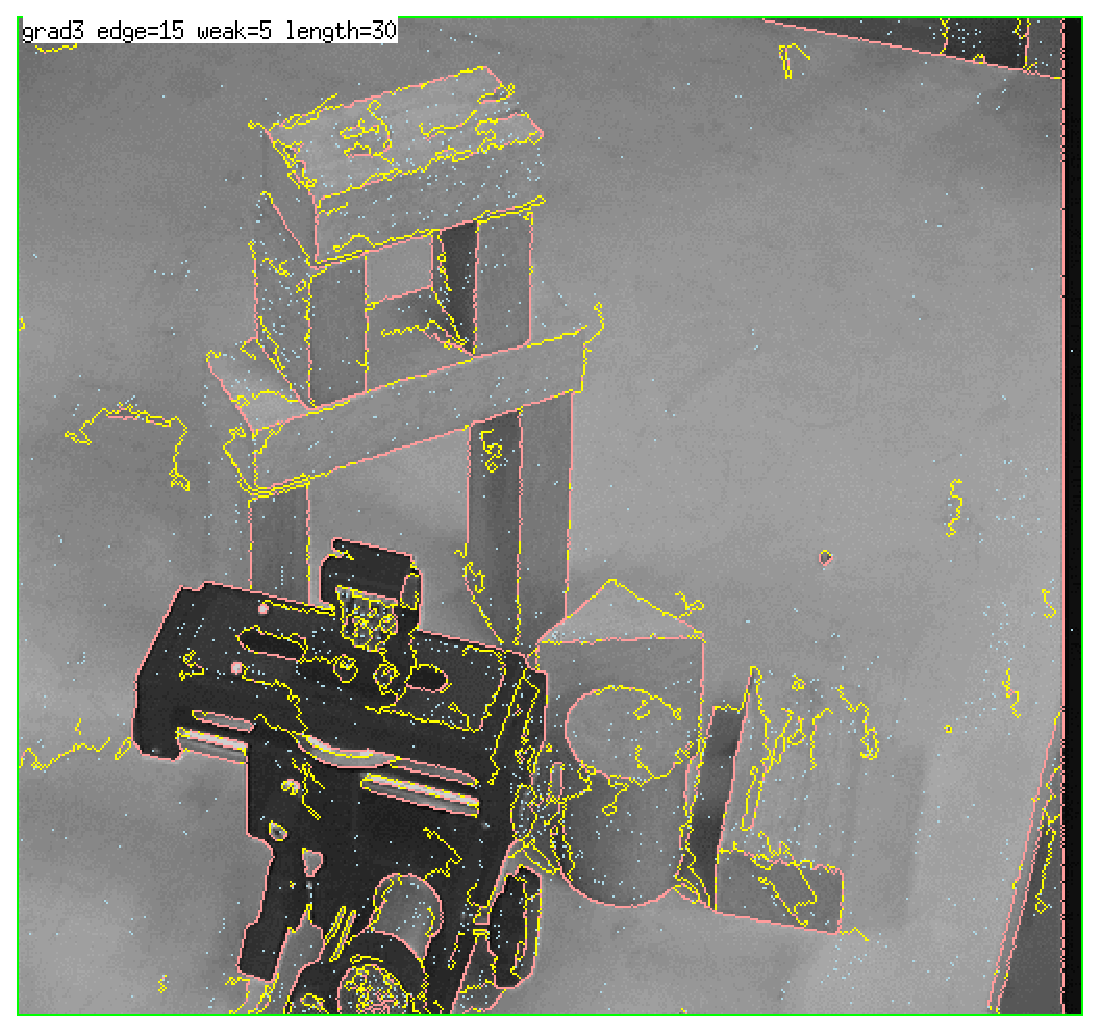
\includegraphics[height=9cm]{fig/block1.edg.ps}
%\epsfile{file=fig/block1.edg.ps,height=9cm}
\caption{Edge Finder and Overlaied Edges}
\end{center}
\end{figure}

\subsection{\label{tracking}トラッキング}
{\tt "vision/correlation"}に元画像とトラッキングしたい画像との
相関を求める関数が定義されている。

\begin{refdesc}
\classdesc{tracking-window}{pixel-image}{x-pos y-pos x-vel y-vel\\
\>pattern-size window-size\\
\>x-win y-win window window-margin\\
\>update threshold half-pattern correlation}{
このクラスは、トラッキング画像を定義する。}

\methoddesc{:correlation}{}{
この画像と元画像との間の相関を返す。}
\methoddesc{:grab}{\&optional (x x-pos) (y y-pos) (sampling 2)}{
画像入力装置から画像を取り込み、その画像の{\bf pixel-image}を返す。}
\methoddesc{:window-rectangle}{val}{
Xwindowの上に四角形を描く。}
\methoddesc{:rectangle}{val}{
Xwindowの上に四角形を描く。}
\methoddesc{:move}{newpos \&aux (newx (aref newpos 0)) (newy (aref newpos 1))}{
トラッキングする位置を{\em newpos}に移動し、新しい画像を取り込む。}
\methoddesc{:track}{display-window \&optional th}{
Xwindowの画像からこの画像をトラッキングする。}
\methoddesc{:serach}{display-window \&optional th}{
Xwindowの画像からこの画像を捜す。}
\methoddesc{:track-and-search}{flag \&optional th}{
この画像をトラッキングする。
もし、トラッキングを失敗したとき、Xwindowからこの画像を捜して
位置を更新する。}

\methoddesc{:pos}{}{
windowの左上位置を返す。}
\methoddesc{:vel}{}{
トラッキング速度を返す。}
\methoddesc{:insidep}{pos \&aux (x (aref pos 0)) (y (aref pos 1))}{
{\em pos}が{\bf tracking-window}の中に含まれるかどうかをチェックする。}
\methoddesc{:update}{\&optional (flag :get)}{
{\tt update}に{\em flag}を設定する。もし、{\em flag}がなければ、
{\tt update}を返す。}
\methoddesc{:prin1}{strm \&rest mesg}{
この{\bf tracking-window}を名前と次元と一緒に表示する。}
\methoddesc{:init}{x y size win-size}{
{\bf tracking-window}を作成する}
\end{refdesc}

\subsection{\label{PBMfile}画像ファイル入出力}
%There are lots of file formats defined for the representation of
%pixel images.
{\tt "vision/pbmfile"}は、Euslispとディスクファイルとの間の
画像データを変換する関数を定義している。
EusLispは、pgm(portable gray-scale map)とppm(portable pixmap)フォーマット
のファイルの読み書きができる。

\begin{refdesc}
\funcdesc{read-pnm}{f \&optional buf0 buf1 buf2}{
{\bf file-stream}の{\em f}で指定されるpgmあるいはppmファイル
を読み込み、{\bf pixel-image}あるいは{\bf color-pixel-image}を返す。
画像ファイルは、asciiでもバイナリーでも可能である。
言い換えれば、P2,P3,P5,P6フォーマットは認識できる。}
\funcdesc{read-pnm-file}{file \&optional buf0 buf1 buf2}{
ファイル名{\em file}で指定されるpgmあるいはppmファイルを読み込む。
%この関数は、{\bf read-ppm}を呼び出す。
}

\funcdesc{write-pgm}{f image  \&optional (depth 255)}{
{\em image}で指定される{\bf pixel-image}を{\bf file-stream}である{\em f}
にバイナリーppmフォーマットで書き込む。
%(この関数は、コメントを追加することで変更できる。)
}
\funcdesc{write-ppm}{f image  \&optional (depth 255)}{
{\em image}で指定される{\bf pixel-image}を{\bf file-stream}である{\em f}
にバイナリーpgmフォーマットで書き込む。}
\funcdesc{write-pnm}{f img}{
{\em img}で指定されるピクセル画像を{\bf file-stream}である{\em f}に書き込む。
もし、{\em img}が{\bf pixel-image}であるなら、バイナリーpgmフォーマットで
書き込み、{\bf color-pixel-image}ならバイナリーppmフォーマットで書き込む。}
\funcdesc{write-pnm-file}{file img}{
ファイル名{\em file}に{\em img}で指定されるピクセル画像を書き込む。
この関数は、{\bf write-pnm}を呼び出す。}

\funcdesc{image::read-raw-image}{file \&optional (x 256) (y x)}{
raw-imageファイルを読み込み、1次元の文字列ベクトルを返す。
%座標系についてなにも前提がない。
raw-imageの次元は、与えられた{\em x}と{\em y}に一致しなければならない。}
\funcdesc{image::write-raw-image}{file imgvec}{
ピクセル値を1バイトのベクトル(文字列)に蓄積した{\em imgvec}を{\em file}
に書き込む。}
\end{refdesc}

\newpage

\section{\label{ManipulatorModel}$B%^%K%T%e%l!<%?(B}
\markright{\arabic{section}. $B%^%K%T%e%l!<%?(B}
\hfill {\em documented by Hiromu Onda}

{\bf rotational-joint}$B%/%i%9$H(B{\bf manipulator}$B%/%i%9$N%$%s%9%?%s%9$+$i%^%K%T%e%l!<%?(B
$B%b%G%k$O9=@.$5$l$k!#(B{\bf rotational-join}$B%/%i%9$O!"(B{\bf body}$B$N%5%V%/%i%9$G$"$j!"(B
$B%^%K%T%e%l!<%?$N4V@\%b%G%k$rDj5A$9$k!#(B
{\bf manipulator}$B$O!"(B{\bf cascaded-coords}$B$N%5%V%/%i%9$G$"$j!"1?F0J}Dx<0$H5U1?F0J}Dx<0$N(B
$B2r$r5a$a$k%a%=%C%I$r;}$C$F$$$k!#(B

$B%^%K%T%e%l!<%?$rDj5A$9$k$K$O!"(B
$B$9$Y$F$N4X@a$r:n@.$7$?8e!"(B{\bf manipulator}$B$K$=$l$i$rE}9g$9$k!#(B

\subsection{
%\label{JointModel}
$B4X@a$N%b%G%k(B}

$B%/%i%9(B{\bf rotational-joint}$B$,4X@a$N%b%G%k$r5-=R$9$k!#(B
$B%/%i%9(B{\bf rotational-joint}$B$O!"(B{\bf body}$B$r%9!<%Q%/%i%9$K;}$A!"(B
$B$=$N7A>u%b%G%k!":BI87O$K2C$($F(B
$B4X@a2sE><4!"2sE>3QEY!"2DF03QEYHO0O!"$J$I$r4IM}$7$F$$$k!#(B
$B<!$N(B{\bf defjoint}$B%^%/%m$K$h$C$F(B{\bf rotational-joint}
$B$N%$%s%9%?%s%9$,:n@.$5$l!"(B{\em joint-name}$B$K%P%$%s%I$5$l$k!#(B
{\bf parent}$B$K$O!"?F$N4X@a$r;XDj$9$k!#(B
$B%Y!<%9$H;X$K$O2DF0<4$r;XDj$9$kI,MW$O$J$$!#(B

\begin{refdesc}
\longdescription{defjoint}{joint-name \&key \= :shape \hspace{10mm}\= {\it body-object} \` [$B%^%/%m(B]\\
% \hspace{70mm} [$B%^%/%m(B]\\
\> :color \> {\it color-id} \hspace{2cm} \= ;0-15 for MMD \\
\> :parent \> {\it parent-joint} \\
\> :axis \> {\it rotational-axis} \>  ; :x, :y or :z \\
\> :offset \> {\it trans-from-parent-joint} \\
\> :low-limit \> {\it joint-angle-limit-low} \\
\> :high-limit \> {\it joint-angle-limit-hight}}{
$B4X@a$N%b%G%k$r5-=R$9$k!#(B}
\end{refdesc}

\subsection{
%\label{MultiJointsManipulator}
$BB?4X@a%^%K%T%e%l!<%?(B}

$B%^%K%T%e%l!<%?%b%G%k$O%/%i%9(B{\bf manipulator}$B$K$h$C$F5-=R$5$l$k!#(B
$B%^%K%T%e%l!<%?%b%G%k$r:n@.$9$k$K$O!"(B
$B<!$N(B{\bf defmanipulator}$B%^%/%m$rMQ$$$k!#(B

\begin{refdesc}
\longdescription{defmanipulator}{manipulator-name \&key \= :class \hspace{2cm} \= {\it manipulator-class} \` [$B%^%/%m(B]\\
%manipulator-class} \hspace{25mm} [$B%^%/%m(B]\\
\> :base \> {\it base-joint} \\
\> :joints \>  {\it list-of-all-joints} \\
\> :hand \> {\it handjoint} \\
\> :left-finger \> {\it left-finger}\\
\> :right-finger \> {\it right-finger}\\
\> :handcoords \> {\it trans-from-hand-to-armsolcoords}\\
\> :toolcoords \> {\it trans-from-armsolcoords-to-toolcoords} \\
\> :open-direction \> {\it finger-open-direction}\\
\> :right-handed  \> {\it righty-or-lefty}}{
$B%^%K%T%e%l!<%?%b%G%k$r:n@.$9$k!#(B}

\classdesc{rotational-joint}{body}{(axis offset high-limit low-limit)}
{6$B<+M3EY%^%K%T%e%l!<%?$N4V@\$r5-=R$9$k!#(B}

\classdesc{manipulator}{cascaded-coords}{(base baseinverse joint angles right-handed hand handcoords\\
\> right-finger left-finger openvec max-span\\
\> toolcoords toolinverse armsolcoords toolinverse armsocoords\\
\> approach grasp affix)}
{$B%Y!<%9$+$i%O%s%I$^$G$N%^%K%T%e%l!<%?$N1?F0$r4IM}$9$k!#(B}

\methoddesc{:newcoords}{newrot \&optional newpos}{ 
$B4X@a3QEY$,8BEY$K<}$^$C$F$$$l$P:BI87O$r(B
{\em newrot}$B$H(B{\em newpos}$B$K99?7$9$k(B 
}
\methoddesc{:armsolcoords }{}{
$B%Y!<%9:BI87O$+$i%O%s%I:BI87O$X$NJQ49!J:BI87O$N%$%s%9%?%s%9!K$r7W;;$7!":n@.$9$k!#(B
%  $B%Y!<%9$+$i%O%s%I$K;j$kJQ49$r5a$a$k(B
}
\methoddesc{:tool}{\&rest msg}{
 $B9)6q:BI87O$rJV$9!"$^$?$OJQ99$9$k(B
}
\methoddesc{:set-tool}{newtool \&optional offset copy}{
 $B9)6q:BI87O(B{\tt toolcoords}$B$K(B{\em newtool}$B$r@_Dj$9$k(B
}
\methoddesc{:reset-tool }{}{
 $B9)6q:BI87O$r=i4|CM$KLa$9(B
}
\methoddesc{:worldcoords }{}{
 $B9)6q:BI87O$N0LCV%Y%/%H%k!"2sE>9TNs!":BI87O$N%o!<%k%II=8=$r5a$a$k(B
}
\methoddesc{:set-coords }{}{
$B=g1?F0$N2r$r5a$a$k$?$a$K!":BI87O$r6/@)E*$K@_Dj$9$k!#(B
% $B0lC6=g%-%M%^$r7W;;$7!"$=$3$+$i$5$i$K3F4X@a3QEY$r5a$a$k(B
}
\methoddesc{:config }{\&optional (a newangles)}{
 6$B$D$N4X@a3QEY$rD>@\$K@_Dj$9$k(B
}
\methoddesc{:park }{}{
 $B=i4|;Q@*$KLa$9(B
}
\methoddesc{:hand}{\&optional (h nil)}{
 $B%O%s%I%*%V%8%'%/%H$rJV$9(B
}
\methoddesc{:handcoords}{}{
 $B%O%s%I:BI87O$N0LCV%Y%/%H%k!"2sE>9TNs!":BI87O$N%o!<%k%II=8=$r5a$a$k(B
}
\methoddesc{:span}{}{
 $B8=:_$N;X$N4V3V$rJV$9(B
}
\methoddesc{:open-fingers}{s \&optional abs \&aux (current (send self :span))}
{
 $B;XI}$rAjBPE*!"@dBPE*$K;XDj$9$k(B
}
\methoddesc{:close-fingers}{}{
 $B;X$r40A4$KJD$8$k(B 
}
\methoddesc{:angles}{\&optional flag}{
 $B8=:_$N;Q@*$N4X@a3QEY$N%j%9%H$rJV$9(B
}

% \methoddesc{:right-handed}{}{
%% $B%=!<%9$=$N$b$N$,$"$j$^$;$s$G$7$?!#(B
% $B1&<j;Q@*!":8<j;Q@*$rA*Br$9$k(B
%}

\methoddesc{:get-approach }{}{
 $B8=:_%"%W%m!<%A$7$F$$$kBP>]$rJV$9(B
}
\methoddesc{:set-approach }{a}{
 $B%"%W%m!<%ABP>](B{\it a}$B$r@_Dj$9$k(B
}
%\methoddesc{:get-grasp}{}{
%(:get-grasp () grasp-config)
%??? 
% $BGD0.;Q@*$K$"$kBP>]J*$rJV$9(B
%}
\methoddesc{:set-grasp}{g}{
 $BGD0.BP>]J*(B{\it g}$B$r;XDj$9$k(B
}
\methoddesc{:get-affix}{}{
 $BGD0.$7$F$$$kJ*BN$rJV$9(B
}
\methoddesc{:affix}{\&optional (grasp)}{
{\bf affixed-object}$B$K(B{\tt grasp}$B$r@_Dj$9$k!#(B
{\tt grasp}$B$O!";RB9$H$7$F(B{\tt handcoords}$B$K4XO"IU$1$i$l$k!#(B
% $BGD0.$r;X<($9$k(B
}
\methoddesc{:unfix}{\&optional (margin 10.0)}{
{\bf affixed-object}$B$K(BNIL$B$r@_Dj$9$k!#(B
{\tt grasp}$B$O!"(B{\tt handcoords}$B$N;RB9%j%9%H$+$i30$5$l$k!#(B
% $BGD0.J*BN$r2rJ|$7$?$3$H$r;X<($9$k(B
}
\longdescription{:create}{\= \&rest args \` [$B%a%=%C%I(B]\\
%\longdescription{:create}{\= \&rest args \hspace{111mm} [$B%a%=%C%I(B]\\
\> \&key \= (:name nm) (:hand h) (:joints j)\\
\> \> (:left-finger lf) (:right-finger rf)\\
\> \> ((:toolcoords tc) (make-coords))\\
\> \> ((:handcoords hc) (make-coords))\\
\> \> ((:base bs) (make-cascoords))\\
\> \> (open-direction (floatvector 0 1 0))\\
\> \> ((:max-span mspan) 100.0)\\
\> \> ((:lefty lft) t)\\
\> \> ((:act a) nil)\\
\> \&allow-other-keys}{
$B?7$7$$%^%K%T%e%l!<%?%*%V%8%'%/%H$r:n@.!"=i4|2=$9$k(B
}
\end{refdesc}

{\bf manipulator}$B%*%V%8%'%/%H$O!"(B
{\bf base$B!"(Bjoints(J1\ldots J6)$B!"(Bhandcoords$B!"(Btoolcoords}
$B$N:BI87O$N7R$,$j$r4IM}$9$k!#(B
%$B?^(B\ref{ManipulatorObject}$B$K(B{\bf manipulator}$B%*%V%8%'%/%H$N%9%m%C%H9=@.$r!"(B
%$BI=(B\ref{ManipulatorMethods}$B$K<u$1IU$1$i$l$k%a%=%C%I$r7G$2$k!#(B
{\bf manipulator}$B%/%i%9$O!"(B{\bf cascaded-coords}$B$N%5%V%/%i%9$G$"$j!"(B
$B$d$O$j!"(B{\bf cascaded-coords}($B$^$?$O(B{\bf body}$B$J$I$N%5%V%/%i%9(B)
$B$G$"$k(B{\bf base}$B$K7k9g$5$l!"(B
{\bf base}$B$+$i(B{\bf toolcoords}($B<j@h:BI87O(B)$B$X$NJQ49$r4IM}$7$F$$$k!#(B
$B$7$?$,$C$F!"(B{\bf manipulator}$B%*%V%8%'%/%H$KBP$7$FAw$i$l$k(B
{\bf :translate$B!"(B:locate$B!"(B:rotate$B!"(B:orient$B!"(B:transform}
$B$J$I$N%a%C%;!<%8$O!"<j@hE@$KBP$7$F:nMQ$9$k!#(B
$B$=$N$H$-F1;~$K(BWRT$B%Q%i%a!<%?$r;XDj$9$l$P!"(B
$B<j@h$O(BWRT$B:BI87O$KBP$7$FF0$/!#(B
$B<!$N%W%m%0%i%`$G$O!"(B{\bf eta3}$B$r(B{\bf manipulator}$B$N%$%s%9%?%s%9$H2>Dj$7$F$$$k!#(B

\begin{verbatim}
$B!!(B(send eta3 :translate #f(0 0 -100))        ;$B<j@h$r(B10cm$B0z$C9~$a$k!!(B
$B!!(B(send eta3 :translate #f(0 0 -100) :world) ;10cm$B2<$2$k(B
$B!!(B(send eta3 :translate #f(0 0 -100)
             (manipulator-base eta3))     ;$B<j@h$r%Y!<%9:BI87O$G(B10cm$B2<$2$k(B
\end{verbatim}

$B$3$l$i$N%a%C%;!<%8$KBP$7$F!"(Bmanipulator$B$O%"!<%`2r$r7W;;$7$F(B6$B$D$N(B
$B4X@a3QEY$r7hDj$9$k!#(B
$B0lHL$K2r$OJ#?tB8:_$9$k$,!"(B{\bf right-handed}($B1&<j7O!":8<j7O(B)
$B$N6hJL!"$*$h$S8=:_$N4X@a3QEY$H$NO"B3@-$K$h$jE,Ev$J2r$,A*Br$5$l$k!#(B
$B$7$+$7!";XDj$5$l$?0LCV!";Q@*$KBP$9$k2r$,B8:_$7$J$$>l9g$d4X@a3Q$,(B
$B8B3&$r1[$($k>l9g$O0\F0!"2sE>$O5/$3$i$:!"7Y9p$,H/$;$i$l$k!#(B

$B%"!<%`2r$N7W;;$O!"<B:]$N%^%K%T%e%l!<%?$KBP1~$7$?(B
$B8D!9$N(Bmanipulator$B%/%i%9$KDj5A$5$l$?(B{\bf :armsol}$B%a%=%C%I$,9T$&!#(B
$B%^%K%T%e%l!<%?$,%o!<%k%I:BI87O$N$I$3$KCV$+$l$F$b$h$$$h$&$K!"(B
$B$^$?!"$I$N$h$&$J9)6q$rMQ$$$F$b$h$$$h$&$K!"%"!<%`2r$O!"(B
{\bf base$B!"(Btoolcoords}$B$H$OFHN)$K!"(Bbase$B:BI87OCf$G$N%O%s%I$N0LCV!";Q@*$K(B
$BBP$7$FM?$($i$l$k!#(B

{\bf base$B!"(BJ1$B!"(BJ2$B!"(B\ldots $B!"(Bhandcoords$B!"(Btoolcoords}$B$N4X78$r?^(B\ref{JointCoords}
$B$K<($9!#(B
$B%o!<%k%I$+$i<j@h$X$NJQ49$r(B$T$$B$H$9$k$H!"(B$T$$B$*$h$S3FItJ,JQ49$O<!$N$h$&$K$7(B
$B$FF@$i$l$k!#(B

$
\begin{array}{ll}
T & = base \cdot J1 \cdot J2 \cdot \ldots 
\cdot J6 \cdot handcoords \cdot toolcoords \\ 
 & = (send \; eta3 \; :worldcoords) \\ 
T_{Jn} & = base \cdot J1\cdot \ldots \cdot Jn \\
 & = (send \; Jn \; :worldcoords) \\
T_{arm} & = J1 \cdot J2 \cdot \ldots \cdot J6 \cdot handcoords \\ 
 & = (send \; eta3 \; :armsol-coords) \\ 
T_{tool} & = J1 \cdot J2 \cdot  \ldots \cdot J6 \cdot handcoords \cdot toolcoords \\ 
 & = (send \; eta3 \; :copy-coords) \\
T_{t} & = toolcoords \\ 
 & = (manipulator-toolcoords \; eta3)\\
T_{t}^{-1} & = toolcoords^{-1} \\ 
 & = (manipulator-toolinverse \; eta3) \\
T_{h} & = handcoords \\ 
 & = (manipulator-handcoords \; eta3)\\
\end{array}$

$B$3$3$G!"(B$T$$B$O%o!<%k%I:BI87O$+$i9)6q:BI87O$^$GJQ49$9$k!#(B

\begin{figure}
\begin{center}
%%% change 2004.12.14 \epsfile{file=/usr/share/src/eus/doc/latex/fig/eta3coords.ps,height=100mm}
\epsfile{file=fig/eta3coords.ps,height=100mm}
\end{center}
\caption{\label{JointCoords}
relation between coordinate systems in a manipulator}

\end{figure}


$B3F4X@a$O!"(BBrep$B$GI=8=$5$l$?4v2?%b%G%k$rJ];}$7$F$$$k!#$7$+$7!"D:E@$N:BI8!"(B
$BJ?LL$NJ}Dx<0$O>o$K8=>u$rH?1G$7$F$$$k$H$O8B$i$J$$!#%^%K%T%e%l!<%?$KBP$9$k(B
$B0\F0!"2sE>$J$I$N%a%C%;!<%8$G$O:BI87O$N99?7$@$1$r9T$$!"D:E@$N:BI8$OJQ2=$7(B
$B$J$$!#$3$l$O!"0\F0!"2sE>$,J#?t2sB3$1$F5/$3$C$?>l9g$N7W;;NL$r8:$i$9$?$a$G(B
$B$"$k!#99?7$O!"%^%K%T%e%l!<%?$K(B{\bf :worldcoords}$B%a%C%;!<%8$rAw$k(B
$B$3$H$G0z$-5/$3$5$l$k!#(B


$B%^%K%T%e%l!<%?$O!"<j@h:BI87O$GF0:n$r;XDj$9$k$3$H$r<g$JL\E*$H$7$F$$$k!#(B
$B4X@a3Q$K$h$k;XDj$K$O(B {\bf :config} $B$rMQ$$$k!#(B
$B0z$-?t$K$O(B6$BMWAG$NNs$rM?$($k!#(B

\begin{verbatim}
$B!!(B (send eta3 :config (float-vector pi/2 pi/2 0 1 0 1))
\end{verbatim}

{\bf :config}$B$O!"3F4X@a3QEY$,2DF0HO0O$K<}$^$C$F$$$k$3$H$r8!::$7$?8e!"(B
$B$=$l$i$r2sE>$5$;$k!#(B
$B$3$N7k2L!"%^%K%T%e%l!<%?$N4IM}$7$F$$$k:BI87O$H(B
$B4X@a3QEY$+$iDj$^$k<B:]$N<j@h$N0LCV;Q@*$H$,0lCW$7$J$/$J$k!#(B
$BN><T$r0lCW$5$;$k$?$a$K$O!"(B{\bf :set-coords}$B%a%C%;!<%8$rAw$k!#(B
{\bf :set-coords}$B$O!"4X@a3QEY$+$i=gJ}8~$N%-%M%^%F%#%/%9$r7W;;$7!"(B
$B:G=*E*$J<j@h:BI87O$KBP$7$F$5$i$K%"!<%`2r$r2r$/!#(B


$BNc(B ETA3$B$N%b%G%k@8@.$H$=$NIA2h(B
\begin{verbatim}
EusLisp 7.27 with Xlib created on Thu Sep 17 14:33:30 1992
(load "view.l")                                ;$B%&%#%s%I%&$r3+$/(B
(load "/usr/local/eus/robot/eta3/eta3build.l") ;ETA3$B$N%b%G%k$r@8@.$9$k(B
(send *viewing* :look #f(2000 2000 2000))      ;$B;kE@$rJQ$($k(B
(send-all (eta3arm-components eta3) :color 1)  ;$BJ*BN$N@~$N?'$r9u$KJQ$($k(B
(send eta3 :config (float-vector 0 (/ -Pi 4.0) Pi/2 0 (/ -Pi 4.0) 0 ))
					       ;ETA3$B$r4X@a3QEY$N;XDj$GF0$+$9(B
(send eta3 :set-coords)                        ;$B>e5-;2>H(B
(draw eta3)                                    ;ETA3$B$rIA2h$9$k(B
\end{verbatim}

\newpage

\newpage

\section{\label{MARS} MARS: マルチ自律ロボットシミュレータ}
\markright{\arabic{section}. MARS}
\hfill {\Large \em (予告)}

\hfill {\em 著者: 国吉 康夫,電総研}

{\bf MARS}は、平面空間内における
マルチ自律移動ロボットのためのシミュレーション環境である。
このプログラムは、Euslispで記述されている。

{\bf 開発状況:}
1995年1月、MARSの発表直前バージョンが電総研内で用いられている。
システムの改善を活発に行い、1995年の上期内に最初のバージョンを
発表する計画である。
その後も、システムの向上をはかり、1996年3月までに安定した状態を
達成したいと望んでいる。
発表の告示はEuslispのメーリングリストや他のインターネットサービス
を通じて行われる予定である。
恐らくライセンスの条件をEuslispから分けるであろう。

{\bf 目的:}
MARSは、単一あるいは複数の移動ロボットで知的ロボットの研究に使用することを
意図してつくられている。たとえば、行動学習やマップ構築や知能収集や
複数ロボット協調や協調学習などである。


\subsection{始め方}
MARSプログラムは、{\bf robot/MARS/ver.XXX}にある。
最初に、".eusrc"ファイルを自分のホームディレクトリにコピーする。
必要があれば変更すること。
(MARSがインストールされているディレクトリのパス名など)

このディレクトリから{\bf eusx}を呼び出す。
すべてのファイルが自動的にロードされ、シミュレータが動作し始める。
windowがオープンされ、初期メッセージが下部windowに現れるまで待つこと。

例:
\begin{verbatim}
Try "SYSTEM"->"Load" menu.
Load "example.bbs".
And "SCL"->"On" menu.
\end{verbatim}

注意:\\
SCL$\rightarrow$"Off" シミュレーションは一時停止するが、GUI処理は続行される。\\
SYSTEM$\rightarrow$"Quit" 最上位のループから抜ける。(mars-loop)により再開できる。\\
SYSTEM$\rightarrow$"Save" 現在の状態をファイルにセーブする。\\
SYSTEM$\rightarrow$"All-Clear" すべてを消し、システムを初期化する。\\
SYSTEM$\rightarrow$"Reset" ロボットの内部状態をリセットするために使用する(特殊目的)。\\

\subsection{システム概要}

\begin{figure}[h]
\begin{center}
%\begin{tabular}{c@\extracolsep{1em}c}
\begin{tabular}{c c}
%%% change 2004.12.14 \epsfile{file=fig/mars.eps,scale=0.3} & % I=;f$HF1$83($KJQ99$7$F!#
%%% change 2004.12.14 \epsfile{file=fig/simst.ps,hscale=0.42,vscale=0.45} \\
\epsfile{file=fig/mars.eps,width=0.4\columnwidth} & % I=;f$HF1$83($KJQ99$7$F!#
\epsfile{file=fig/simst.ps,width=0.6\columnwidth} \\
\end{tabular}
\caption{\label{MARSOverview} MARS windowの表示例(左)と
プログラムの構造(右)}
\end{center}
\end{figure}

MARSを始めたとき、図~\ref{MARSOverview}(左)に示されるような
メインwindowを見ることができる。MARSは、図~\ref{MARSOverview}(右)
のようなモジュールアーキテクチャを採用している。
それは、物理シミュレーションモジュールとロボット制御モジュールと
ユーザーインターフェースモジュールとユーザーが定義したグローバル
制御ループにより構成されている。

{\bf 物理シミュレーション:}
現在の物理シミュレーションモジュールは、4つのタイプのオブジェクトを
処理している。
{\bf wall} (固定障害物), {\bf block} (移動障害物), {\bf
robot-body} (活動オブジェクト)と{\bf magic-block} (経験学習するための
特別な報酬を与えるオブジェクト)である。

\begin{figure}
\begin{center}
%\begin{tabular}{c@\extracolsep{1em}c}
\begin{tabular}{c c}
%%% change 2004.12.14 \epsfile{file=fig/robot-ui2.ps,hscale=0.5,vscale=0.5} &
%%% change 2004.12.14 \epsfile{file=fig/robot-st2.ps,scale=0.4} \\
\epsfile{file=fig/robot-ui2.ps,width=0.5\columnwidth} &
\epsfile{file=fig/robot-st2.ps,width=0.5\columnwidth} \\
\end{tabular}
\end{center}
\caption{\label{fig:robotst}ロボットの内部構造(左)と
ビヘービアベーストロボットの構成例(右)}
\end{figure}

{\bf ロボットモデル:}
物理的シミュレーションモジュールとロボット制御モジュールとの
間のインターフェースである。
いくつもの{\bf robot}モデルを生成することができ、
擬似並列でシミュレートできる。
{\bf robot}はそれぞれ、{\bf robot-body}と{\bf robot-brain}の
のモジュールの組みで構成される。
{\bf robot-body}は、ロボットの物理的な性質を定義し、
{\bf robot-brain}はロボットの行動を定義する。

{\bf センサモデル:}
ユーザーは、{\bf robot-body}のどこにでもいくつものセンサを
選択して取り付けることができる。
現在、実現されているセンサモデルは、以下のものである。
{\bf 距離センサ} (走行距離), {\bf 角度センサ} (回転角),
{\bf 接触センサ}, {\bf 赤外線センサ}, {\bf レーザセンサ} (超音波), 
{\bf 視覚センサ} (object-name-sensor)。
現在のバージョンでは、ノイズや不確定要素について考えていない。

{\bf ロボット知能:}
{\bf robot-brain}は、シミュレートしたセンサデータを処理したり
行動命令を生成するためにユーザーで定義されたモジュールである。
センサデータを受け、行動命令を出力しなければならない。
付け加えて、リエントラントプログラムとして書かれていて、
グローバル制御ループによって送られる{\bf :step}メッセージ
によって時間分割されなければならない。
これらの拘束に合う限り、ユーザーはどんな認識アーキテクチャも
採用することができる。
システムは、デフォルトとしてビヘービアベースト型のアーキテクチャ
の例を備えている。

{\bf GUI:}
{\bf MARS}のメインwindowは、システムを制御するためにいくつかのボタンを
持つメニューバーを持っている。
また、システムは物理環境を生成/変更するための内部グラフィックエディタ
を持っている。
ファイルに対してエージェント定義と一緒に物理環境を読み書きできる。

{\bf ネットワーク拡張:}
{\bf robot-brain}は、非同期ソケット通信を通して外部プロセス
との接続を構築することができる。
この場合、ユーザーは{\bf remote-brain}を記述するために任意の言語(C,
Prolog, Scheme, Perl, etc...)を使用することができる。
非同期接続のおかげで、ユーザーは時間分割について少しも気にする必要が無い。

{\bf 経験学習機能:}
{\bf MARS}は、ロボットが経験学習するための幾つかの特殊機能を備えている。
報酬を与えるオブジェクトや報酬センサ(報酬値をロボットに送るもの)
や報酬ログ(システム全体の報酬の統計を計算するもの)である。

%
\cleardoublepage
\markboth{Euslisp version \eusversion リファレンスマニュアル}{Index}
\footnotesize
\printindex
\end{document}

